%&preformat-disser
\RequirePackage[l2tabu,orthodox]{nag} % Раскомментировав, можно в логе получать рекомендации относительно правильного использования пакетов и предупреждения об устаревших и нерекомендуемых пакетах
% Формат А4, 14pt (ГОСТ Р 7.0.11-2011, 5.3.6)
\documentclass[a4paper,14pt,oneside,openany]{memoir}

%% Режим черновика
\makeatletter
\@ifundefined{c@draft}{
  \newcounter{draft}
  \setcounter{draft}{0}  % 0 --- чистовик (максимальное соблюдение ГОСТ)
                         % 1 --- черновик (отклонения от ГОСТ, но быстрая сборка итоговых PDF)
}{}
\makeatother

%% Использование пакета pscyr, при его наличии
\makeatletter
\@ifundefined{c@usepscyr}{
  \newcounter{usepscyr}
  \setcounter{usepscyr}{1}  % 0 --- не использовать пакет pscyr
                            % 1 --- использовать пакет pscyr, при его наличии 
}{}
\makeatother

%% Библиография

%% Внимание! При использовании bibtex8 необходимо удалить все
%% цитирования из  ../common/characteristic.tex
\makeatletter
\@ifundefined{c@bibliosel}{
  \newcounter{bibliosel}
  \setcounter{bibliosel}{1}           % 0 --- встроенная реализация с загрузкой файла через движок bibtex8; 1 --- реализация пакетом biblatex через движок biber
}{}
\makeatother

%%% Предкомпиляция tikz рисунков для ускорения работы %%%
\makeatletter
\@ifundefined{c@imgprecompile}{
  \newcounter{imgprecompile}
  \setcounter{imgprecompile}{0}   % 0 --- без предкомпиляции;
                                  % 1 --- пользоваться предварительно скомпилированными pdf вместо генерации заново из tikz
}{}
\makeatother
            % общие настройки шаблона
%%% Проверка используемого TeX-движка %%%
\RequirePackage{ifxetex, ifluatex}
\newif\ifxetexorluatex   % определяем новый условный оператор (http://tex.stackexchange.com/a/47579)
\ifxetex
    \xetexorluatextrue
\else
    \ifluatex
        \xetexorluatextrue
    \else
        \xetexorluatexfalse
    \fi
\fi

\newif\ifsynopsis           % Условие, проверяющее, что документ --- автореферат

\RequirePackage{etoolbox}[2015/08/02]               % Для продвинутой проверки разных условий
\providebool{presentation}

%%% Поля и разметка страницы %%%
\usepackage{pdflscape}                              % Для включения альбомных страниц
\usepackage{geometry}                               % Для последующего задания полей

%%% Математические пакеты %%%
\usepackage{amsthm,amsmath,amscd}   % Математические дополнения от AMS
\usepackage{amsfonts,amssymb}       % Математические дополнения от AMS
\usepackage{mathtools}              % Добавляет окружение multlined
\usepackage{xfrac}                  % Красивые дроби
\usepackage[
    locale = DE,
    list-separator       = {;\,},
    list-final-separator = {;\,},
    list-pair-separator  = {;\,},
    range-phrase         = {\text{\ensuremath{-}}},
    % quotient-mode        = fraction, % красивые дроби могут не соответствовать ГОСТ
    fraction-function    = \sfrac,
    separate-uncertainty,
    ]{siunitx}                      % Размерности SI
\sisetup{inter-unit-product = \ensuremath{{}\cdot{}}}

% Кириллица в нумерации subequations
% Для правильной работы требуется выполнение сразу после загрузки пакетов
\patchcmd{\subequations}{\def\theequation{\theparentequation\alph{equation}}}
{\def\theequation{\theparentequation\asbuk{equation}}}
{\typeout{subequations patched}}{\typeout{subequations not patched}}

%%%% Установки для размера шрифта 14 pt %%%%
%% Формирование переменных и констант для сравнения (один раз для всех подключаемых файлов)%%
%% должно располагаться до вызова пакета fontspec или polyglossia, потому что они сбивают его работу
\newlength{\curtextsize}
\newlength{\bigtextsize}
\setlength{\bigtextsize}{13.9pt}

\makeatletter
%\show\f@size                                       % неплохо для отслеживания, но вызывает стопорение процесса, если документ компилируется без команды  -interaction=nonstopmode
\setlength{\curtextsize}{\f@size pt}
\makeatother

%%% Кодировки и шрифты %%%
\ifxetexorluatex
    \usepackage{polyglossia}[2014/05/21]            % Поддержка многоязычности (fontspec подгружается автоматически)
\else
   %%% Решение проблемы копирования текста в буфер кракозябрами
    \ifnumequal{\value{usealtfont}}{0}{}{
        \input glyphtounicode.tex
        \input glyphtounicode-cmr.tex %from pdfx package
        \pdfgentounicode=1
    }
    \usepackage{cmap}                               % Улучшенный поиск русских слов в полученном pdf-файле
    \ifnumequal{\value{usealtfont}}{2}{}{
        \defaulthyphenchar=127                      % Если стоит до fontenc, то переносы не впишутся в выделяемый текст при копировании его в буфер обмена
    }
    \usepackage{textcomp}
    \usepackage[T1,T2A]{fontenc}                    % Поддержка русских букв
    \ifnumequal{\value{usealtfont}}{1}{% Используется pscyr, при наличии
        \IfFileExists{pscyr.sty}{\usepackage{pscyr}}{}  % Подключение pscyr
    }{}
    \usepackage[utf8]{inputenc}[2014/04/30]         % Кодировка utf8
    \usepackage[english, russian]{babel}[2014/03/24]% Языки: русский, английский
    \ifnumequal{\value{usealtfont}}{2}{
        % http://dxdy.ru/post1238763.html#p1238763
        \usepackage[scaled=0.960]{XCharter}[2017/12/19] % Подключение русифицированных шрифтов XCharter
        \usepackage[charter, vvarbb, scaled=1.048]{newtxmath}[2017/12/14]
        \setDisplayskipStretch{-0.078}
    }{}
\fi

%%% Оформление абзацев %%%
\usepackage{indentfirst}                            % Красная строка

%%% Цвета %%%
\ifpresentation
\else
    \usepackage[dvipsnames, table, hyperref]{xcolor} % Совместимо с tikz
\fi

%%% Таблицы %%%
\usepackage{longtable,ltcaption}                    % Длинные таблицы
\usepackage{multirow,makecell}                      % Улучшенное форматирование таблиц

%%% Общее форматирование
\usepackage{soulutf8}                               % Поддержка переносоустойчивых подчёркиваний и зачёркиваний
\usepackage{icomma}                                 % Запятая в десятичных дробях

%%% Оптимизация расстановки переносов и длины последней строки абзаца
\IfFileExists{impnattypo.sty}{% проверка установленности пакета impnattypo
    \ifluatex
        \ifnumequal{\value{draft}}{1}{% Черновик
            \usepackage[hyphenation, lastparline, nosingleletter, homeoarchy,
            rivers, draft]{impnattypo}
        }{% Чистовик
            \usepackage[hyphenation, lastparline, nosingleletter]{impnattypo}
        }
    \else
        \usepackage[hyphenation, lastparline]{impnattypo}
    \fi
}{}

%%% Гиперссылки %%%
\usepackage{hyperref}[2012/11/06]

%%% Изображения %%%
\usepackage{graphicx}[2014/04/25]                   % Подключаем пакет работы с графикой

%%% Счётчики %%%
\usepackage[figure,table]{totalcount}               % Счётчик рисунков и таблиц
\usepackage{totcount}                               % Пакет создания счётчиков на основе последнего номера подсчитываемого элемента (может требовать дважды компилировать документ)
\usepackage{totpages}                               % Счётчик страниц, совместимый с hyperref (ссылается на номер последней страницы). Желательно ставить последним пакетом в преамбуле

%%% Продвинутое управление групповыми ссылками (пока только формулами) %%%
\ifpresentation
\else
    \ifxetexorluatex
        \usepackage{cleveref}                           % cleveref корректно считывает язык из настроек polyglossia
    \else
        \usepackage[russian]{cleveref}                  % cleveref имеет сложности со считыванием языка из babel. Такое решение русификации вывода выбрано вместо определения в documentclass из опасности что-то лишнее передать во все остальные пакеты, включая библиографию.
    \fi
    \creflabelformat{equation}{#2#1#3}                  % Формат по умолчанию ставил круглые скобки вокруг каждого номера ссылки, теперь просто номера ссылок без какого-либо дополнительного оформления
    \crefrangelabelformat{equation}{#3#1#4\cyrdash#5#2#6}   % Интервалы в русском языке принято делать через тире, если иное не оговорено

    % решение проблемы с "и" в \labelcref
    % https://tex.stackexchange.com/a/455124/104425
    \ifxetexorluatex
        \DeclareTextSymbol{\cyri}\UnicodeEncodingName{"0438} % и
    \fi

    % Добавление возможности использования пробелов в \labelcref
    % https://tex.stackexchange.com/a/340502/104425
    \usepackage{kvsetkeys}
    \makeatletter
    \let\org@@cref\@cref
    \renewcommand*{\@cref}[2]{%
        \edef\process@me{%
            \noexpand\org@@cref{#1}{\zap@space#2 \@empty}%
        }\process@me
    }
    \makeatother
\fi

\ifnumequal{\value{draft}}{1}{% Черновик
    \usepackage[firstpage]{draftwatermark}
    \SetWatermarkText{DRAFT}
    \SetWatermarkFontSize{14pt}
    \SetWatermarkScale{15}
    \SetWatermarkAngle{45}
}{}

%%% Исправление положения якорей подписей (под)рисунков %%%
% Без hypcap и патча, при клике по ссылке на подрисунок, просмотрщик pdf прыгает "к подписи" а не "к рисунку".
% Подробнее: https://github.com/AndreyAkinshin/Russian-Phd-LaTeX-Dissertation-Template/issues/238
% (!) Даже с патчем, если мешать в одной фиге разные типы подфиг (subbottom и subcaption) - ссылки всё равно будут работать неправильно  (см. https://www.overleaf.com/read/czmbmmtnqrrg ).
\ifpresentation
\else
    \usepackage[all]{hypcap}

    \makeatletter
    \ltx@ifclasslater{memoir}{2018/12/13}{
        % Предполагается, что в следующей версии класс будет исправлен
        \typeout{Assuming this version of memoir is free from the jumping-to-caption bug.}
    }{
        \RequirePackage{xpatch}

        \newcommand\mem@step@subcounter{\refstepcounter{sub\@captype}\@contkeep}

        \xpatchcmd{\@memsubbody}%
        {\refstepcounter{sub\@captype}\@contkeep}% search pattern
        {}% replacement
        {\typeout{@memsubbody is patched}}%
        {\typeout{@memsubbody is NOT patched}}%

        \xpatchcmd{\@memcontsubbody}%
        {\refstepcounter{sub\@captype}\@contkeep}% pattern
        {}% replacement
        {\typeout{@memcontsubbody is patched}}%
        {\typeout{@memcontsubbody is NOT patched}}%

        \xpatchcmd{\@memsubfloat}%
        {\vbox\bgroup}% search pattern
        {\vbox\bgroup\mem@step@subcounter}% replacement
        {\typeout{@memsubfloat patch is ok}}%
        {\typeout{@memsubfloat patch is NOT ok}}%

        \xpatchcmd{\subcaption}%
        {\refstepcounter{sub\@captype}}% search pattern
        {\H@refstepcounter{sub\@captype}}% replacement
        {\typeout{subcaption second patch is ok}}%
        {\typeout{subcaption second patch is NOT ok}}%
    }
    \makeatother
\fi

%%% Цитата, не приводимая в автореферате:
% возможно, актуальна только для biblatex
%\newcommand{\citeinsynopsis}[1]{\ifsynopsis\else ~\cite{#1} \fi}

%% Векторная графика

\usepackage{tikz}                   % Продвинутый пакет векторной графики
\usetikzlibrary{chains}             % Для примера tikz рисунка
\usetikzlibrary{shapes.geometric}   % Для примера tikz рисунка
\usetikzlibrary{shapes.symbols}     % Для примера tikz рисунка
\usetikzlibrary{arrows}             % Для примера tikz рисунка

% если текущий процесс запущен библиотекой tikz-external, то прекомпиляция должна быть включена
\ifdefined\tikzexternalrealjob
    \setcounter{imgprecompile}{1}
\fi

\ifnumequal{\value{imgprecompile}}{1}{% Только если у нас включена предкомпиляция
    \usetikzlibrary{external}   % подключение возможности предкомпиляции
    \tikzexternalize[prefix=images/cache/] % activate! % здесь можно указать отдельную папку для скомпилированных файлов
    \ifxetex
        \tikzset{external/up to date check={diff}}
    \fi
}{}
         % Пакеты общие для диссертации и автореферата
\synopsisfalse                      % Этот документ --- не автореферат
%%% Прикладные пакеты %%% 
%\usepackage{calc}               % Пакет для расчётов параметров, например длины

%%% Для добавления Стр. над номерами страниц в оглавлении
%%% http://tex.stackexchange.com/a/306950
\usepackage{afterpage}

\usepackage{tikz}                   % Продвинутый пакет векторной графики
\usetikzlibrary{chains}             % Для примера tikz рисунка
\usetikzlibrary{shapes.geometric}   % Для примера tikz рисунка
\usetikzlibrary{shapes.symbols}     % Для примера tikz рисунка
\usetikzlibrary{arrows}             % Для примера tikz рисунка
\ifnumequal{\value{imgprecompile}}{1}{% Только если у нас включена предкомпиляция
    \usetikzlibrary{external}   % подключение возможности предкомпиляции
    \tikzexternalize[prefix=Dissertation/images/] % activate! % здесь можно указать отдельную папку для скомпилированных файлов
    \ifxetex
        \tikzset{external/up to date check={diff}}
    \fi
}{}
    % Пакеты для диссертации
\usepackage{tabularx, tabu, tabulary}  %таблицы с автоматически подбирающейся шириной столбцов

% Листинги с исходным кодом программ
\usepackage{fancyvrb}
\usepackage{listings}

% Плавающие окружения. во многом лучше пакета float
\usepackage{floatrow}

% Русская традиция начертания греческих букв
%\usepackage{upgreek} % прямые греческие ради русской традиции   % Пакеты для специфических пользовательских задач

%%%%%%%%%%%%%%%%%%%%%%%%%%%%%%%%%%%%%%%%%%%%%%%%%%%%%%
%%%% Файл упрощённых настроек шаблона диссертации %%%%
%%%%%%%%%%%%%%%%%%%%%%%%%%%%%%%%%%%%%%%%%%%%%%%%%%%%%%

%%% Инициализирование переменных, не трогать!  %%%
\newcounter{intvl}
\newcounter{otstup}
\newcounter{contnumeq}
\newcounter{contnumfig}
\newcounter{contnumtab}
\newcounter{pgnum}
\newcounter{chapstyle}
\newcounter{headingdelim}
\newcounter{headingalign}
\newcounter{headingsize}
\newcounter{tabcap}
\newcounter{tablaba}
\newcounter{tabtita}
%%%%%%%%%%%%%%%%%%%%%%%%%%%%%%%%%%%%%%%%%%%%%%%%%%

%%% Область упрощённого управления оформлением %%%

%% Интервал между заголовками и между заголовком и текстом
% Заголовки отделяют от текста сверху и снизу тремя интервалами (ГОСТ Р 7.0.11-2011, 5.3.5)
\setcounter{intvl}{3}               % Коэффициент кратности к размеру шрифта

%% Отступы у заголовков в тексте
\setcounter{otstup}{0}              % 0 --- без отступа; 1 --- абзацный отступ

%% Нумерация формул, таблиц и рисунков
\setcounter{contnumeq}{0}           % Нумерация формул: 0 --- пораздельно (во введении подряд, без номера раздела); 1 --- сквозная нумерация по всей диссертации
\setcounter{contnumfig}{0}          % Нумерация рисунков: 0 --- пораздельно (во введении подряд, без номера раздела); 1 --- сквозная нумерация по всей диссертации
\setcounter{contnumtab}{1}          % Нумерация таблиц: 0 --- пораздельно (во введении подряд, без номера раздела); 1 --- сквозная нумерация по всей диссертации

%% Оглавление
\setcounter{pgnum}{1}               % 0 --- номера страниц никак не обозначены; 1 --- Стр. над номерами страниц (дважды компилировать после изменения)
\settocdepth{subsection}            % до какого уровня подразделов выносить в оглавление
\setsecnumdepth{subsection}         % до какого уровня нумеровать подразделы


%% Текст и форматирование заголовков
\setcounter{chapstyle}{1}           % 0 --- разделы только под номером; 1 --- разделы с названием "Глава" перед номером
\setcounter{headingdelim}{1}        % 0 --- номер отделен пропуском в 1em или \quad; 1 --- номера разделов и приложений отделены точкой с пробелом, подразделы пропуском без точки; 2 --- номера разделов, подразделов и приложений отделены точкой с пробелом.

%% Выравнивание заголовков в тексте
\setcounter{headingalign}{0}        % 0 --- по центру; 1 --- по левому краю

%% Размеры заголовков в тексте
\setcounter{headingsize}{0}         % 0 --- по ГОСТ, все всегда 14 пт; 1 --- пропорционально изменяющийся размер в зависимости от базового шрифта

%% Подпись таблиц
\setcounter{tabcap}{0}              % 0 --- по ГОСТ, номер таблицы и название разделены тире, выровнены по левому краю, при необходимости на нескольких строках; 1 --- подпись таблицы не по ГОСТ, на двух и более строках, дальнейшие настройки: 
%Выравнивание первой строки, с подписью и номером
\setcounter{tablaba}{2}             % 0 --- по левому краю; 1 --- по центру; 2 --- по правому краю
%Выравнивание строк с самим названием таблицы
\setcounter{tabtita}{1}             % 0 --- по левому краю; 1 --- по центру; 2 --- по правому краю
%Разделитель записи «Таблица #» и названия таблицы
\newcommand{\tablabelsep}{space}   % space = пробел, period = точка (определены в подключенных пакетах)

%% Подпись рисунков
%Разделитель записи «Рисунок #» и названия рисунка
\newcommand{\figlabelsep}{emdash}   % emdash = тире, определён в common/styles; period = точка определён в подключенных пакетах

%%% Цвета гиперссылок %%%
% Latex color definitions: http://latexcolor.com/
\definecolor{linkcolor}{rgb}{0.9,0,0}
\definecolor{citecolor}{rgb}{0,0.6,0}
\definecolor{urlcolor}{rgb}{0,0,1}
%\definecolor{linkcolor}{rgb}{0,0,0} %black
%\definecolor{citecolor}{rgb}{0,0,0} %black
%\definecolor{urlcolor}{rgb}{0,0,0} %black      % Упрощённые настройки шаблона

% Новые переменные, которые могут использоваться во всём проекте
% ГОСТ 7.0.11-2011
% 9.2 Оформление текста автореферата диссертации
% 9.2.1 Общая характеристика работы включает в себя следующие основные структурные
% элементы:
% актуальность темы исследования;
\newcommand{\actualityTXT}{Актуальность темы.}
% степень ее разработанности;
\newcommand{\progressTXT}{Степень разработанности темы.}
% цели и задачи;
\newcommand{\aimTXT}{Целью}
\newcommand{\tasksTXT}{задачи}
% научную новизну;
\newcommand{\noveltyTXT}{Научная новизна:}
% теоретическую и практическую значимость работы;
%\newcommand{\influenceTXT}{Теоретическая и практическая значимость}
% или чаще используют просто
\newcommand{\influenceTXT}{Практическая значимость}
% методологию и методы исследования;
\newcommand{\methodsTXT}{Методология и методы исследования.}
% положения, выносимые на защиту;
\newcommand{\defpositionsTXT}{Основные положения, выносимые на~защиту:}
% степень достоверности и апробацию результатов.
\newcommand{\reliabilityTXT}{Достоверность}
\newcommand{\probationTXT}{Апробация работы.}

\newcommand{\contributionTXT}{Личный вклад.}
\newcommand{\publicationsTXT}{Публикации.}


\newcommand{\bibtitleauthor}{Публикации автора по теме диссертации}
\newcommand{\bibtitleauthorvak}{В изданиях из списка ВАК РФ}
\newcommand{\bibtitleauthorscopus}{В изданиях, входящих в международную базу цитирования Scopus}
\newcommand{\bibtitleauthorwos}{В изданиях, входящих в международную базу цитирования Web of Science}
\newcommand{\bibtitleauthorothers}{В прочих изданиях}
\newcommand{\bibtitleauthorconf}{В сборниках трудов конференций}
\newcommand{\fullbibtitle}{Список литературы} % (ГОСТ Р 7.0.11-2011, 4)
         % Новые переменные, для всего проекта

%%% Основные сведения %%%
\newcommand{\thesisAuthorLastName}{\todo{Фамилия}}
\newcommand{\thesisAuthorOtherNames}{\todo{Имя Отчество}}
\newcommand{\thesisAuthorInitials}{\todo{И.\,О.}}
\newcommand{\thesisAuthor}             % Диссертация, ФИО автора
{%
    \texorpdfstring{% \texorpdfstring takes two arguments and uses the first for (La)TeX and the second for pdf
        \thesisAuthorLastName~\thesisAuthorOtherNames% так будет отображаться на титульном листе или в тексте, где будет использоваться переменная
    }{%
        \thesisAuthorLastName, \thesisAuthorOtherNames% эта запись для свойств pdf-файла. В таком виде, если pdf будет обработан программами для сбора библиографических сведений, будет правильно представлена фамилия.
    }
}
\newcommand{\thesisAuthorShort}        % Диссертация, ФИО автора инициалами
{\thesisAuthorInitials~\thesisAuthorLastName}
%\newcommand{\thesisUdk}                % Диссертация, УДК
%{\todo{xxx.xxx}}
\newcommand{\thesisTitle}              % Диссертация, название
{\todo{Название диссертационной работы}}
\newcommand{\thesisSpecialtyNumber}    % Диссертация, специальность, номер
{\todo{XX.XX.XX}}
\newcommand{\thesisSpecialtyTitle}     % Диссертация, специальность, название
{\todo{Название специальности}}
%% \newcommand{\thesisSpecialtyTwoNumber} % Диссертация, вторая специальность, номер
%% {\todo{XX.XX.XX}}
%% \newcommand{\thesisSpecialtyTwoTitle}  % Диссертация, вторая специальность, название
%% {\todo{Название специальности}}
\newcommand{\thesisDegree}             % Диссертация, ученая степень
{\todo{кандидата физико-математических наук}}
\newcommand{\thesisDegreeShort}        % Диссертация, ученая степень, краткая запись
{\todo{канд. физ.-мат. наук}}
\newcommand{\thesisCity}               % Диссертация, город написания диссертации
{\todo{Город}}
\newcommand{\thesisYear}               % Диссертация, год написания диссертации
{\todo{20XX}}
\newcommand{\thesisOrganization}       % Диссертация, организация
{\todo{Название учреждения, в~котором выполнялась данная диссертационная работа}}
\newcommand{\thesisOrganizationShort}  % Диссертация, краткое название организации для доклада
{\todo{НазУчДисРаб}}

\newcommand{\thesisInOrganization}     % Диссертация, организация в предложном падеже: Работа выполнена в ...
{\todo{учреждении, в~котором выполнялась данная диссертационная работа}}

%% \newcommand{\supervisorDead}{}           % Рисовать рамку вокруг фамилии
\newcommand{\supervisorFio}              % Научный руководитель, ФИО
{\todo{Фамилия Имя Отчество}}
\newcommand{\supervisorRegalia}          % Научный руководитель, регалии
{\todo{уч. степень, уч. звание}}
\newcommand{\supervisorFioShort}         % Научный руководитель, ФИО
{\todo{И.\,О.~Фамилия}}
\newcommand{\supervisorRegaliaShort}     % Научный руководитель, регалии
{\todo{уч.~ст.,~уч.~зв.}}

%% \newcommand{\supervisorTwoDead}{}        % Рисовать рамку вокруг фамилии
%% \newcommand{\supervisorTwoFio}           % Второй научный руководитель, ФИО
%% {\todo{Фамилия Имя Отчество}}
%% \newcommand{\supervisorTwoRegalia}       % Второй научный руководитель, регалии
%% {\todo{уч. степень, уч. звание}}
%% \newcommand{\supervisorTwoFioShort}      % Второй научный руководитель, ФИО
%% {\todo{И.\,О.~Фамилия}}
%% \newcommand{\supervisorTwoRegaliaShort}  % Второй научный руководитель, регалии
%% {\todo{уч.~ст.,~уч.~зв.}}

\newcommand{\opponentOneFio}           % Оппонент 1, ФИО
{\todo{Фамилия Имя Отчество}}
\newcommand{\opponentOneRegalia}       % Оппонент 1, регалии
{\todo{доктор физико-математических наук, профессор}}
\newcommand{\opponentOneJobPlace}      % Оппонент 1, место работы
{\todo{Не очень длинное название для места работы}}
\newcommand{\opponentOneJobPost}       % Оппонент 1, должность
{\todo{старший научный сотрудник}}

\newcommand{\opponentTwoFio}           % Оппонент 2, ФИО
{\todo{Фамилия Имя Отчество}}
\newcommand{\opponentTwoRegalia}       % Оппонент 2, регалии
{\todo{кандидат физико-математических наук}}
\newcommand{\opponentTwoJobPlace}      % Оппонент 2, место работы
{\todo{Основное место работы c длинным длинным длинным длинным названием}}
\newcommand{\opponentTwoJobPost}       % Оппонент 2, должность
{\todo{старший научный сотрудник}}

%% \newcommand{\opponentThreeFio}         % Оппонент 3, ФИО
%% {\todo{Фамилия Имя Отчество}}
%% \newcommand{\opponentThreeRegalia}     % Оппонент 3, регалии
%% {\todo{кандидат физико-математических наук}}
%% \newcommand{\opponentThreeJobPlace}    % Оппонент 3, место работы
%% {\todo{Основное место работы c длинным длинным длинным длинным названием}}
%% \newcommand{\opponentThreeJobPost}     % Оппонент 3, должность
%% {\todo{старший научный сотрудник}}

\newcommand{\leadingOrganizationTitle} % Ведущая организация, дополнительные строки
{\todo{Федеральное государственное бюджетное образовательное учреждение высшего профессионального образования с~длинным длинным длинным длинным названием}}

\newcommand{\defenseDate}              % Защита, дата
{\todo{DD mmmmmmmm YYYY~г.~в~XX часов}}
\newcommand{\defenseCouncilNumber}     % Защита, номер диссертационного совета
{\todo{Д\,123.456.78}}
\newcommand{\defenseCouncilTitle}      % Защита, учреждение диссертационного совета
{\todo{Название учреждения}}
\newcommand{\defenseCouncilAddress}    % Защита, адрес учреждение диссертационного совета
{\todo{Адрес}}
\newcommand{\defenseCouncilPhone}      % Телефон для справок
{\todo{+7~(0000)~00-00-00}}

\newcommand{\defenseSecretaryFio}      % Секретарь диссертационного совета, ФИО
{\todo{Фамилия Имя Отчество}}
\newcommand{\defenseSecretaryRegalia}  % Секретарь диссертационного совета, регалии
{\todo{д-р~физ.-мат. наук}}            % Для сокращений есть ГОСТы, например: ГОСТ Р 7.0.12-2011 + http://base.garant.ru/179724/#block_30000

\newcommand{\synopsisLibrary}          % Автореферат, название библиотеки
{\todo{Название библиотеки}}
\newcommand{\synopsisDate}             % Автореферат, дата рассылки
{\todo{DD mmmmmmmm YYYY года}}

% To avoid conflict with beamer class use \providecommand
\providecommand{\keywords}%            % Ключевые слова для метаданных PDF диссертации и автореферата
{}
             % Основные сведения
%%% Кодировки и шрифты %%%
\ifxetexorluatex
    \setmainlanguage[babelshorthands=true]{russian}    % Язык по-умолчанию русский с поддержкой приятных команд пакета babel
    \setotherlanguage{english}                         % Дополнительный язык = английский (в американской вариации по-умолчанию)

    % Проверка существования шрифтов. Недоступна в pdflatex
    \ifnumequal{\value{fontfamily}}{1}{
        \IfFontExistsTF{Times New Roman}{}{\setcounter{fontfamily}{0}}
    }{}
    \ifnumequal{\value{fontfamily}}{2}{
        \IfFontExistsTF{LiberationSerif}{}{\setcounter{fontfamily}{0}}
    }{}

    \ifnumequal{\value{fontfamily}}{0}{                    % Семейство шрифтов CMU. Используется как fallback
        \setmonofont{CMU Typewriter Text}                  % моноширинный шрифт
        \newfontfamily\cyrillicfonttt{CMU Typewriter Text} % моноширинный шрифт для кириллицы
        \defaultfontfeatures{Ligatures=TeX}                % стандартные лигатуры TeX, замены нескольких дефисов на тире и т. п. Настройки моноширинного шрифта должны идти до этой строки, чтобы при врезках кода программ в коде не применялись лигатуры и замены дефисов
        \setmainfont{CMU Serif}                            % Шрифт с засечками
        \newfontfamily\cyrillicfont{CMU Serif}             % Шрифт с засечками для кириллицы
        \setsansfont{CMU Sans Serif}                       % Шрифт без засечек
        \newfontfamily\cyrillicfontsf{CMU Sans Serif}      % Шрифт без засечек для кириллицы
    }

    \ifnumequal{\value{fontfamily}}{1}{                    % Семейство MS шрифтов
        \setmonofont{Courier New}                          % моноширинный шрифт
        \newfontfamily\cyrillicfonttt{Courier New}         % моноширинный шрифт для кириллицы
        \defaultfontfeatures{Ligatures=TeX}                % стандартные лигатуры TeX, замены нескольких дефисов на тире и т. п. Настройки моноширинного шрифта должны идти до этой строки, чтобы при врезках кода программ в коде не применялись лигатуры и замены дефисов
        \setmainfont{Times New Roman}                      % Шрифт с засечками
        \newfontfamily\cyrillicfont{Times New Roman}       % Шрифт с засечками для кириллицы
        \setsansfont{Arial}                                % Шрифт без засечек
        \newfontfamily\cyrillicfontsf{Arial}               % Шрифт без засечек для кириллицы
    }

    \ifnumequal{\value{fontfamily}}{2}{                    % Семейство шрифтов Liberation (https://pagure.io/liberation-fonts)
        \setmonofont{LiberationMono}[Scale=MatchLowercase] % моноширинный шрифт
        \newfontfamily\cyrillicfonttt{LiberationMono}[     % моноширинный шрифт для кириллицы
            Scale=MatchLowercase]
        \defaultfontfeatures{Ligatures=TeX}                % стандартные лигатуры TeX, замены нескольких дефисов на тире и т. п. Настройки моноширинного шрифта должны идти до этой строки, чтобы при врезках кода программ в коде не применялись лигатуры и замены дефисов
        \setmainfont{LiberationSerif}                      % Шрифт с засечками
        \newfontfamily\cyrillicfont{LiberationSerif}       % Шрифт с засечками для кириллицы
        \setsansfont{LiberationSans}                       % Шрифт без засечек
        \newfontfamily\cyrillicfontsf{LiberationSans}      % Шрифт без засечек для кириллицы
    }

\else
    \ifnumequal{\value{usealtfont}}{1}{% Используется pscyr, при наличии
        \IfFileExists{pscyr.sty}{\renewcommand{\rmdefault}{ftm}}{}
    }{}
\fi
            % Определение шрифтов (частичное)
%%% Кодировки и шрифты %%%
\ifxetexorluatex
    \setmainlanguage[babelshorthands=true]{russian}  % Язык по-умолчанию русский с поддержкой приятных команд пакета babel
    \setotherlanguage{english}                       % Дополнительный язык = английский (в американской вариации по-умолчанию)
    \setmonofont{Courier New}
    \newfontfamily\cyrillicfonttt{Courier New}
    \ifXeTeX
        \defaultfontfeatures{Ligatures=TeX,Mapping=tex-text}
    \else
        \defaultfontfeatures{Ligatures=TeX}
    \fi
    \setmainfont{Times New Roman}
    \newfontfamily\cyrillicfont{Times New Roman}
    \setsansfont{Arial}
    \newfontfamily\cyrillicfontsf{Arial}
\else
    \IfFileExists{pscyr.sty}{\renewcommand{\rmdefault}{ftm}}{}
\fi

%%% Подписи %%%
\captionsetup{%
singlelinecheck=off,                % Многострочные подписи, например у таблиц
skip=2pt,                           % Вертикальная отбивка между подписью и содержимым рисунка или таблицы определяется ключом
justification=centering,            % Центрирование подписей, заданных командой \caption
}

%%% Рисунки %%%
\DeclareCaptionLabelSeparator*{emdash}{~--- }             % (ГОСТ 2.105, 4.3.1)
\captionsetup[figure]{labelsep=emdash,position=bottom}

%%% Таблицы %%%
\ifthenelse{\equal{\thetabcap}{0}}{%
    \newcommand{\tabcapalign}{\raggedright}  % по левому краю страницы или аналога parbox
}{}

\ifthenelse{\equal{\thetablaba}{0} \AND \equal{\thetabcap}{1}}{%
    \newcommand{\tabcapalign}{\raggedright}  % по левому краю страницы или аналога parbox
}{}

\ifthenelse{\equal{\thetablaba}{1} \AND \equal{\thetabcap}{1}}{%
    \newcommand{\tabcapalign}{\centering}    % по центру страницы или аналога parbox
}{}

\ifthenelse{\equal{\thetablaba}{2} \AND \equal{\thetabcap}{1}}{%
    \newcommand{\tabcapalign}{\raggedleft}   % по правому краю страницы или аналога parbox
}{}

\ifthenelse{\equal{\thetabtita}{0} \AND \equal{\thetabcap}{1}}{%
    \newcommand{\tabtitalign}{\raggedright}  % по левому краю страницы или аналога parbox
}{}

\ifthenelse{\equal{\thetabtita}{1} \AND \equal{\thetabcap}{1}}{%
    \newcommand{\tabtitalign}{\centering}    % по центру страницы или аналога parbox
}{}

\ifthenelse{\equal{\thetabtita}{2} \AND \equal{\thetabcap}{1}}{%
    \newcommand{\tabtitalign}{\raggedleft}   % по правому краю страницы или аналога parbox
}{}

\DeclareCaptionFormat{tablenocaption}{\tabcapalign #1\strut}        % Наименование таблицы отсутствует
\ifthenelse{\equal{\thetabcap}{0}}{%
    \DeclareCaptionFormat{tablecaption}{\tabcapalign #1#2#3}
    \captionsetup[table]{labelsep=emdash}                       % тире как разделитель идентификатора с номером от наименования
}{%
    \DeclareCaptionFormat{tablecaption}{\tabcapalign #1#2\par%  % Идентификатор таблицы на отдельной строке
        \tabtitalign{#3}}                                       % Наименование таблицы строкой ниже
    \captionsetup[table]{labelsep=space}                        % пробельный разделитель идентификатора с номером от наименования
}
\captionsetup[table]{format=tablecaption,singlelinecheck=off,position=top,skip=0pt}  % многострочные наименования и прочее
\DeclareCaptionLabelFormat{continued}{Продолжение таблицы~#2}

%%% Подписи подрисунков %%%
\renewcommand{\thesubfigure}{\asbuk{subfigure}}           % Буквенные номера подрисунков
\captionsetup[subfigure]{font={normalsize},               % Шрифт подписи названий подрисунков (не отличается от основного)
    labelformat=brace,                                    % Формат обозначения подрисунка
    justification=centering,                              % Выключка подписей (форматирование), один из вариантов            
}
%\DeclareCaptionFont{font12pt}{\fontsize{12pt}{13pt}\selectfont} % объявляем шрифт 12pt для использования в подписях, тут же надо интерлиньяж объявлять, если не наследуется
%\captionsetup[subfigure]{font={font12pt}}                 % Шрифт подписи названий подрисунков (всегда 12pt)

%%% Настройки гиперссылок %%%
\ifLuaTeX
    \hypersetup{
        unicode,                % Unicode encoded PDF strings
    }
\fi

\hypersetup{
    linktocpage=true,           % ссылки с номера страницы в оглавлении, списке таблиц и списке рисунков
%    linktoc=all,                % both the section and page part are links
%    pdfpagelabels=false,        % set PDF page labels (true|false)
    plainpages=false,           % Forces page anchors to be named by the Arabic form  of the page number, rather than the formatted form
    colorlinks,                 % ссылки отображаются раскрашенным текстом, а не раскрашенным прямоугольником, вокруг текста
    linkcolor={linkcolor},      % цвет ссылок типа ref, eqref и подобных
    citecolor={citecolor},      % цвет ссылок-цитат
    urlcolor={urlcolor},        % цвет гиперссылок
%    hidelinks,                  % Hide links (removing color and border)
    pdftitle={\thesisTitle},    % Заголовок
    pdfauthor={\thesisAuthor},  % Автор
    pdfsubject={\thesisSpecialtyNumber\ \thesisSpecialtyTitle},      % Тема
%    pdfcreator={Создатель},     % Создатель, Приложение
%    pdfproducer={Производитель},% Производитель, Производитель PDF
    pdfkeywords={\keywords},    % Ключевые слова
    pdflang={ru},
}
\ifthenelse{\equal{\thedraft}{1}}{% Черновик
    \hypersetup{
        draft,
    }
}{}

%%% Шаблон %%%
\DeclareRobustCommand{\todo}{\textcolor{red}}       % решаем проблему превращения названия цвета в результате \MakeUppercase, http://tex.stackexchange.com/a/187930/79756 , \DeclareRobustCommand protects \todo from expanding inside \MakeUppercase
\AtBeginDocument{%
    \setlength{\parindent}{2.5em}                   % Абзацный отступ. Должен быть одинаковым по всему тексту и равен пяти знакам (ГОСТ Р 7.0.11-2011, 5.3.7).
}

%%% Списки %%%
% Используем короткое тире (endash) для ненумерованных списков (ГОСТ 2.105-95, пункт 4.1.7, требует дефиса, но так лучше смотрится)
\renewcommand{\labelitemi}{\normalfont\bfseries{--}}

% Перечисление строчными буквами латинского алфавита (ГОСТ 2.105-95, 4.1.7)
%\renewcommand{\theenumi}{\alph{enumi}}
%\renewcommand{\labelenumi}{\theenumi)} 

% Перечисление строчными буквами русского алфавита (ГОСТ 2.105-95, 4.1.7)
%\makeatletter
%\AddEnumerateCounter{\asbuk}{\russian@alph}{щ}      % Управляем списками/перечислениями через пакет enumitem, а он 'не знает' про asbuk, потому 'учим' его
%\makeatother
%\renewcommand{\theenumi}{\asbuk{enumi}}
%\renewcommand{\labelenumi}{\theenumi)} 

\setlist{nosep,%                                    % Единый стиль для всех списков (пакет enumitem), без дополнительных интервалов.
    labelindent=\parindent,leftmargin=*%            % Каждый пункт, подпункт и перечисление записывают с абзацного отступа (ГОСТ 2.105-95, 4.1.8)
}
           % Стили общие для диссертации и автореферата
%%% Переопределение именований, если иначе не сработает %%%
%\gappto\captionsrussian{
%    \renewcommand{\chaptername}{Глава}
%    \renewcommand{\appendixname}{Приложение} % (ГОСТ Р 7.0.11-2011, 5.7)
%}

%%% Изображения %%%
\graphicspath{{images/}{Dissertation/images/}}         % Пути к изображениям

%%% Интервалы %%%
%% По ГОСТ Р 7.0.11-2011, пункту 5.3.6 требуется полуторный интервал
%% Реализация средствами класса (на основе setspace) ближе к типографской классике.
%% И правит сразу и в таблицах (если со звёздочкой)
%\DoubleSpacing*     % Двойной интервал
\OnehalfSpacing*    % Полуторный интервал
%\setSpacing{1.42}   % Полуторный интервал, подобный Ворду (возможно, стоит включать вместе с предыдущей строкой)

%%% Макет страницы %%%
% Выставляем значения полей (ГОСТ 7.0.11-2011, 5.3.7)
\geometry{a4paper, top=2cm, bottom=2cm, left=2.5cm, right=1cm, nofoot, nomarginpar} %, heightrounded, showframe
\setlength{\topskip}{0pt}   %размер дополнительного верхнего поля
\setlength{\footskip}{12.3pt} % снимет warning, согласно https://tex.stackexchange.com/a/334346

%%% Выравнивание и переносы %%%
%% http://tex.stackexchange.com/questions/241343/what-is-the-meaning-of-fussy-sloppy-emergencystretch-tolerance-hbadness
%% http://www.latex-community.org/forum/viewtopic.php?p=70342#p70342
\tolerance 1414
\hbadness 1414
\emergencystretch 1.5em % В случае проблем регулировать в первую очередь
\hfuzz 0.3pt
\vfuzz \hfuzz
%\raggedbottom
%\sloppy                 % Избавляемся от переполнений
\clubpenalty=10000      % Запрещаем разрыв страницы после первой строки абзаца
\widowpenalty=10000     % Запрещаем разрыв страницы после последней строки абзаца
\brokenpenalty=4991     % Ограничение на разрыв страницы, если строка заканчивается переносом

%%% Блок управления параметрами для выравнивания заголовков в тексте %%%
\newlength{\otstuplen}
\setlength{\otstuplen}{\theotstup\parindent}
\ifnumequal{\value{headingalign}}{0}{% выравнивание заголовков в тексте
    \newcommand{\hdngalign}{\centering}                % по центру
    \newcommand{\hdngaligni}{}% по центру
    \setlength{\otstuplen}{0pt}
}{%
    \newcommand{\hdngalign}{}                 % по левому краю
    \newcommand{\hdngaligni}{\hspace{\otstuplen}}      % по левому краю
} % В обоих случаях вроде бы без переноса, как и надо (ГОСТ Р 7.0.11-2011, 5.3.5)

%%% Оглавление %%%
\renewcommand{\cftchapterdotsep}{\cftdotsep}                % отбивка точками до номера страницы начала главы/раздела

%% Переносить слова в заголовке не допускается (ГОСТ Р 7.0.11-2011, 5.3.5). Заголовки в оглавлении должны точно повторять заголовки в тексте (ГОСТ Р 7.0.11-2011, 5.2.3). Прямого указания на запрет переносов в оглавлении нет, но по той же логике невнесения искажений в смысл, лучше в оглавлении не переносить:
\setrmarg{2.55em plus1fil}                             %To have the (sectional) titles in the ToC, etc., typeset ragged right with no hyphenation
\renewcommand{\cftchapterpagefont}{\normalfont}        % нежирные номера страниц у глав в оглавлении
\renewcommand{\cftchapterleader}{\cftdotfill{\cftchapterdotsep}}% нежирные точки до номеров страниц у глав в оглавлении
%\renewcommand{\cftchapterfont}{}                       % нежирные названия глав в оглавлении

\ifnumgreater{\value{headingdelim}}{0}{%
    \renewcommand\cftchapteraftersnum{.\space}       % добавляет точку с пробелом после номера раздела в оглавлении
}{}
\ifnumgreater{\value{headingdelim}}{1}{%
    \renewcommand\cftsectionaftersnum{.\space}       % добавляет точку с пробелом после номера подраздела в оглавлении
    \renewcommand\cftsubsectionaftersnum{.\space}    % добавляет точку с пробелом после номера подподраздела в оглавлении
    \renewcommand\cftsubsubsectionaftersnum{.\space} % добавляет точку с пробелом после номера подподподраздела в оглавлении
    \AfterEndPreamble{% без этого polyglossia сама всё переопределяет
        \setsecnumformat{\csname the#1\endcsname.\space}
    }
}{%
    \AfterEndPreamble{% без этого polyglossia сама всё переопределяет
        \setsecnumformat{\csname the#1\endcsname\quad}
    }
}

\renewcommand*{\cftappendixname}{\appendixname\space} % Слово Приложение в оглавлении

%%% Колонтитулы %%%
% Порядковый номер страницы печатают на середине верхнего поля страницы (ГОСТ Р 7.0.11-2011, 5.3.8)
\makeevenhead{plain}{}{\thepage}{}
\makeoddhead{plain}{}{\thepage}{}
\makeevenfoot{plain}{}{}{}
\makeoddfoot{plain}{}{}{}
\pagestyle{plain}

%%% добавить Стр. над номерами страниц в оглавлении
%%% http://tex.stackexchange.com/a/306950
\newif\ifendTOC

\newcommand*{\tocheader}{
\ifnumequal{\value{pgnum}}{1}{%
    \ifendTOC\else\hbox to \linewidth%
      {\noindent{}~\hfill{Стр.}}\par%
      \ifnumless{\value{page}}{3}{}{%
        \vspace{0.5\onelineskip}
      }
      \afterpage{\tocheader}
    \fi%
}{}%
}%

%%% Оформление заголовков глав, разделов, подразделов %%%
%% Работа должна быть выполнена ... размером шрифта 12-14 пунктов (ГОСТ Р 7.0.11-2011, 5.3.8). То есть не должно быть надписей шрифтом более 14. Так и поставим.
%% Эти установки будут давать одинаковый результат независимо от выбора базовым шрифтом 12 пт или 14 пт
\newcommand{\basegostsectionfont}{\fontsize{14pt}{16pt}\selectfont\bfseries}

\makechapterstyle{thesisgost}{%
    \chapterstyle{default}
    \setlength{\beforechapskip}{0pt}
    \setlength{\midchapskip}{0pt}
    \setlength{\afterchapskip}{\theintvl\curtextsize}
    \renewcommand*{\chapnamefont}{\basegostsectionfont}
    \renewcommand*{\chapnumfont}{\basegostsectionfont}
    \renewcommand*{\chaptitlefont}{\basegostsectionfont}
    \renewcommand*{\chapterheadstart}{}
    \ifnumgreater{\value{headingdelim}}{0}{%
        \renewcommand*{\afterchapternum}{.\space}   % добавляет точку с пробелом после номера раздела
    }{%
        \renewcommand*{\afterchapternum}{\quad}     % добавляет \quad после номера раздела
    }
    \renewcommand*{\printchapternum}{\hdngaligni\hdngalign\chapnumfont \thechapter}
    \renewcommand*{\printchaptername}{}
    \renewcommand*{\printchapternonum}{\hdngaligni\hdngalign}
}

\makeatletter
\makechapterstyle{thesisgostchapname}{%
    \chapterstyle{thesisgost}
    \renewcommand*{\printchapternum}{\chapnumfont \thechapter}
    \renewcommand*{\printchaptername}{\hdngaligni\hdngalign\chapnamefont \@chapapp} %
}
\makeatother

\chapterstyle{thesisgost}

\setsecheadstyle{\basegostsectionfont\hdngalign}
\setsecindent{\otstuplen}

\setsubsecheadstyle{\basegostsectionfont\hdngalign}
\setsubsecindent{\otstuplen}

\setsubsubsecheadstyle{\basegostsectionfont\hdngalign}
\setsubsubsecindent{\otstuplen}

\sethangfrom{\noindent #1} %все заголовки подразделов центрируются с учетом номера, как block

\ifnumequal{\value{chapstyle}}{1}{%
    \chapterstyle{thesisgostchapname}
    \renewcommand*{\cftchaptername}{\chaptername\space} % будет вписано слово Глава перед каждым номером раздела в оглавлении
}{}%

%%% Интервалы между заголовками
\setbeforesecskip{\theintvl\curtextsize}% Заголовки отделяют от текста сверху и снизу тремя интервалами (ГОСТ Р 7.0.11-2011, 5.3.5).
\setaftersecskip{\theintvl\curtextsize}
\setbeforesubsecskip{\theintvl\curtextsize}
\setaftersubsecskip{\theintvl\curtextsize}
\setbeforesubsubsecskip{\theintvl\curtextsize}
\setaftersubsubsecskip{\theintvl\curtextsize}

%%% Вертикальные интервалы глав (\chapter) в оглавлении как и у заголовков
% раскомментировать следующие 2
% \setlength{\cftbeforechapterskip}{0pt plus 0pt}   % ИЛИ эти 2 строки из учебника
% \renewcommand*{\insertchapterspace}{}
% или эту
% \renewcommand*{\cftbeforechapterskip}{0em}


%%% Блок дополнительного управления размерами заголовков
\ifnumequal{\value{headingsize}}{1}{% Пропорциональные заголовки и базовый шрифт 14 пт
    \renewcommand{\basegostsectionfont}{\large\bfseries}
    \renewcommand*{\chapnamefont}{\Large\bfseries}
    \renewcommand*{\chapnumfont}{\Large\bfseries}
    \renewcommand*{\chaptitlefont}{\Large\bfseries}
}{}

%%% Счётчики %%%

%% Упрощённые настройки шаблона диссертации: нумерация формул, таблиц, рисунков
\ifnumequal{\value{contnumeq}}{1}{%
    \counterwithout{equation}{chapter} % Убираем связанность номера формулы с номером главы/раздела
}{}
\ifnumequal{\value{contnumfig}}{1}{%
    \counterwithout{figure}{chapter}   % Убираем связанность номера рисунка с номером главы/раздела
}{}
\ifnumequal{\value{contnumtab}}{1}{%
    \counterwithout{table}{chapter}    % Убираем связанность номера таблицы с номером главы/раздела
}{}

\AtBeginDocument{
%% регистрируем счётчики в системе totcounter
    \regtotcounter{totalcount@figure}
    \regtotcounter{totalcount@table}       % Если иным способом поставить в преамбуле то ошибка в числе таблиц
    \regtotcounter{TotPages}               % Если иным способом поставить в преамбуле то ошибка в числе страниц
    \newtotcounter{totalappendix}
    \newtotcounter{totalchapter}
}
  % Стили для диссертации
% для вертикального центрирования ячеек в tabulary
\def\zz{\ifx\[$\else\aftergroup\zzz\fi}
%$ \] % <-- чиним подсветку синтаксиса в некоторых редакторах
\def\zzz{\setbox0\lastbox
\dimen0\dimexpr\extrarowheight + \ht0-\dp0\relax
\setbox0\hbox{\raise-.5\dimen0\box0}%
\ht0=\dimexpr\ht0+\extrarowheight\relax
\dp0=\dimexpr\dp0+\extrarowheight\relax 
\box0
}

\lstdefinelanguage{Renhanced}%
{keywords={abbreviate,abline,abs,acos,acosh,action,add1,add,%
        aggregate,alias,Alias,alist,all,anova,any,aov,aperm,append,apply,%
        approx,approxfun,apropos,Arg,args,array,arrows,as,asin,asinh,%
        atan,atan2,atanh,attach,attr,attributes,autoload,autoloader,ave,%
        axis,backsolve,barplot,basename,besselI,besselJ,besselK,besselY,%
        beta,binomial,body,box,boxplot,break,browser,bug,builtins,bxp,by,%
        c,C,call,Call,case,cat,category,cbind,ceiling,character,char,%
        charmatch,check,chol,chol2inv,choose,chull,class,close,cm,codes,%
        coef,coefficients,co,col,colnames,colors,colours,commandArgs,%
        comment,complete,complex,conflicts,Conj,contents,contour,%
        contrasts,contr,control,helmert,contrib,convolve,cooks,coords,%
        distance,coplot,cor,cos,cosh,count,fields,cov,covratio,wt,CRAN,%
        create,crossprod,cummax,cummin,cumprod,cumsum,curve,cut,cycle,D,%
        data,dataentry,date,dbeta,dbinom,dcauchy,dchisq,de,debug,%
        debugger,Defunct,default,delay,delete,deltat,demo,de,density,%
        deparse,dependencies,Deprecated,deriv,description,detach,%
        dev2bitmap,dev,cur,deviance,off,prev,,dexp,df,dfbetas,dffits,%
        dgamma,dgeom,dget,dhyper,diag,diff,digamma,dim,dimnames,dir,%
        dirname,dlnorm,dlogis,dnbinom,dnchisq,dnorm,do,dotplot,double,%
        download,dpois,dput,drop,drop1,dsignrank,dt,dummy,dump,dunif,%
        duplicated,dweibull,dwilcox,dyn,edit,eff,effects,eigen,else,%
        emacs,end,environment,env,erase,eval,equal,evalq,example,exists,%
        exit,exp,expand,expression,External,extract,extractAIC,factor,%
        fail,family,fft,file,filled,find,fitted,fivenum,fix,floor,for,%
        For,formals,format,formatC,formula,Fortran,forwardsolve,frame,%
        frequency,ftable,ftable2table,function,gamma,Gamma,gammaCody,%
        gaussian,gc,gcinfo,gctorture,get,getenv,geterrmessage,getOption,%
        getwd,gl,glm,globalenv,gnome,GNOME,graphics,gray,grep,grey,grid,%
        gsub,hasTsp,hat,heat,help,hist,home,hsv,httpclient,I,identify,if,%
        ifelse,Im,image,\%in\%,index,influence,measures,inherits,install,%
        installed,integer,interaction,interactive,Internal,intersect,%
        inverse,invisible,IQR,is,jitter,kappa,kronecker,labels,lapply,%
        layout,lbeta,lchoose,lcm,legend,length,levels,lgamma,library,%
        licence,license,lines,list,lm,load,local,locator,log,log10,log1p,%
        log2,logical,loglin,lower,lowess,ls,lsfit,lsf,ls,machine,Machine,%
        mad,mahalanobis,make,link,margin,match,Math,matlines,mat,matplot,%
        matpoints,matrix,max,mean,median,memory,menu,merge,methods,min,%
        missing,Mod,mode,model,response,mosaicplot,mtext,mvfft,na,nan,%
        names,omit,nargs,nchar,ncol,NCOL,new,next,NextMethod,nextn,%
        nlevels,nlm,noquote,NotYetImplemented,NotYetUsed,nrow,NROW,null,%
        numeric,\%o\%,objects,offset,old,on,Ops,optim,optimise,optimize,%
        options,or,order,ordered,outer,package,packages,page,pairlist,%
        pairs,palette,panel,par,parent,parse,paste,path,pbeta,pbinom,%
        pcauchy,pchisq,pentagamma,persp,pexp,pf,pgamma,pgeom,phyper,pico,%
        pictex,piechart,Platform,plnorm,plogis,plot,pmatch,pmax,pmin,%
        pnbinom,pnchisq,pnorm,points,poisson,poly,polygon,polyroot,pos,%
        postscript,power,ppoints,ppois,predict,preplot,pretty,Primitive,%
        print,prmatrix,proc,prod,profile,proj,prompt,prop,provide,%
        psignrank,ps,pt,ptukey,punif,pweibull,pwilcox,q,qbeta,qbinom,%
        qcauchy,qchisq,qexp,qf,qgamma,qgeom,qhyper,qlnorm,qlogis,qnbinom,%
        qnchisq,qnorm,qpois,qqline,qqnorm,qqplot,qr,Q,qty,qy,qsignrank,%
        qt,qtukey,quantile,quasi,quit,qunif,quote,qweibull,qwilcox,%
        rainbow,range,rank,rbeta,rbind,rbinom,rcauchy,rchisq,Re,read,csv,%
        csv2,fwf,readline,socket,real,Recall,rect,reformulate,regexpr,%
        relevel,remove,rep,repeat,replace,replications,report,require,%
        resid,residuals,restart,return,rev,rexp,rf,rgamma,rgb,rgeom,R,%
        rhyper,rle,rlnorm,rlogis,rm,rnbinom,RNGkind,rnorm,round,row,%
        rownames,rowsum,rpois,rsignrank,rstandard,rstudent,rt,rug,runif,%
        rweibull,rwilcox,sample,sapply,save,scale,scan,scan,screen,sd,se,%
        search,searchpaths,segments,seq,sequence,setdiff,setequal,set,%
        setwd,show,sign,signif,sin,single,sinh,sink,solve,sort,source,%
        spline,splinefun,split,sqrt,stars,start,stat,stem,step,stop,%
        storage,strstrheight,stripplot,strsplit,structure,strwidth,sub,%
        subset,substitute,substr,substring,sum,summary,sunflowerplot,svd,%
        sweep,switch,symbol,symbols,symnum,sys,status,system,t,table,%
        tabulate,tan,tanh,tapply,tempfile,terms,terrain,tetragamma,text,%
        time,title,topo,trace,traceback,transform,tri,trigamma,trunc,try,%
        ts,tsp,typeof,unclass,undebug,undoc,union,unique,uniroot,unix,%
        unlink,unlist,unname,untrace,update,upper,url,UseMethod,var,%
        variable,vector,Version,vi,warning,warnings,weighted,weights,%
        which,while,window,write,\%x\%,x11,X11,xedit,xemacs,xinch,xor,%
        xpdrows,xy,xyinch,yinch,zapsmall,zip},%
    otherkeywords={!,!=,~,$,*,\%,\&,\%/\%,\%*\%,\%\%,<-,<<-},%$
    alsoother={._$},%$
    sensitive,%
    morecomment=[l]\#,%
    morestring=[d]",%
    morestring=[d]'% 2001 Robert Denham
}%

%решаем проблему с кириллицей в комментариях (в pdflatex) https://tex.stackexchange.com/a/103712
\lstset{extendedchars=true,keepspaces=true,literate={Ö}{{\"O}}1
    {Ä}{{\"A}}1
    {Ü}{{\"U}}1
    {ß}{{\ss}}1
    {ü}{{\"u}}1
    {ä}{{\"a}}1
    {ö}{{\"o}}1
    {~}{{\textasciitilde}}1
    {а}{{\selectfont\char224}}1
    {б}{{\selectfont\char225}}1
    {в}{{\selectfont\char226}}1
    {г}{{\selectfont\char227}}1
    {д}{{\selectfont\char228}}1
    {е}{{\selectfont\char229}}1
    {ё}{{\"e}}1
    {ж}{{\selectfont\char230}}1
    {з}{{\selectfont\char231}}1
    {и}{{\selectfont\char232}}1
    {й}{{\selectfont\char233}}1
    {к}{{\selectfont\char234}}1
    {л}{{\selectfont\char235}}1
    {м}{{\selectfont\char236}}1
    {н}{{\selectfont\char237}}1
    {о}{{\selectfont\char238}}1
    {п}{{\selectfont\char239}}1
    {р}{{\selectfont\char240}}1
    {с}{{\selectfont\char241}}1
    {т}{{\selectfont\char242}}1
    {у}{{\selectfont\char243}}1
    {ф}{{\selectfont\char244}}1
    {х}{{\selectfont\char245}}1
    {ц}{{\selectfont\char246}}1
    {ч}{{\selectfont\char247}}1
    {ш}{{\selectfont\char248}}1
    {щ}{{\selectfont\char249}}1
    {ъ}{{\selectfont\char250}}1
    {ы}{{\selectfont\char251}}1
    {ь}{{\selectfont\char252}}1
    {э}{{\selectfont\char253}}1
    {ю}{{\selectfont\char254}}1
    {я}{{\selectfont\char255}}1
    {А}{{\selectfont\char192}}1
    {Б}{{\selectfont\char193}}1
    {В}{{\selectfont\char194}}1
    {Г}{{\selectfont\char195}}1
    {Д}{{\selectfont\char196}}1
    {Е}{{\selectfont\char197}}1
    {Ё}{{\"E}}1
    {Ж}{{\selectfont\char198}}1
    {З}{{\selectfont\char199}}1
    {И}{{\selectfont\char200}}1
    {Й}{{\selectfont\char201}}1
    {К}{{\selectfont\char202}}1
    {Л}{{\selectfont\char203}}1
    {М}{{\selectfont\char204}}1
    {Н}{{\selectfont\char205}}1
    {О}{{\selectfont\char206}}1
    {П}{{\selectfont\char207}}1
    {Р}{{\selectfont\char208}}1
    {С}{{\selectfont\char209}}1
    {Т}{{\selectfont\char210}}1
    {У}{{\selectfont\char211}}1
    {Ф}{{\selectfont\char212}}1
    {Х}{{\selectfont\char213}}1
    {Ц}{{\selectfont\char214}}1
    {Ч}{{\selectfont\char215}}1
    {Ш}{{\selectfont\char216}}1
    {Щ}{{\selectfont\char217}}1
    {Ъ}{{\selectfont\char218}}1
    {Ы}{{\selectfont\char219}}1
    {Ь}{{\selectfont\char220}}1
    {Э}{{\selectfont\char221}}1
    {Ю}{{\selectfont\char222}}1
    {Я}{{\selectfont\char223}}1
    {і}{{\selectfont\char105}}1
    {ї}{{\selectfont\char168}}1
    {є}{{\selectfont\char185}}1
    {ґ}{{\selectfont\char160}}1
    {І}{{\selectfont\char73}}1
    {Ї}{{\selectfont\char136}}1
    {Є}{{\selectfont\char153}}1
    {Ґ}{{\selectfont\char128}}1
}

% Ширина текста минус ширина надписи 999
\newlength{\twless}
\newlength{\lmarg}
\setlength{\lmarg}{\widthof{999}}   % ширина надписи 999
\setlength{\twless}{\textwidth-\lmarg}

\lstset{ %
%    language=R,                     %  Язык указать здесь, если во всех листингах преимущественно один язык, в результате часть настроек может пойти только для этого языка
    numbers=left,                   % where to put the line-numbers
    numberstyle=\fontsize{12pt}{14pt}\selectfont\color{Gray},  % the style that is used for the line-numbers
    firstnumber=1,                  % в этой и следующей строках задаётся поведение нумерации 5, 10, 15...
    stepnumber=5,                   % the step between two line-numbers. If it's 1, each line will be numbered
    numbersep=5pt,                  % how far the line-numbers are from the code
    backgroundcolor=\color{white},  % choose the background color. You must add \usepackage{color}
    showspaces=false,               % show spaces adding particular underscores
    showstringspaces=false,         % underline spaces within strings
    showtabs=false,                 % show tabs within strings adding particular underscores
    frame=leftline,                 % adds a frame of different types around the code
    rulecolor=\color{black},        % if not set, the frame-color may be changed on line-breaks within not-black text (e.g. commens (green here))
    tabsize=2,                      % sets default tabsize to 2 spaces
    captionpos=t,                   % sets the caption-position to top
    breaklines=true,                % sets automatic line breaking
    breakatwhitespace=false,        % sets if automatic breaks should only happen at whitespace
%    title=\lstname,                 % show the filename of files included with \lstinputlisting;
    % also try caption instead of title
    basicstyle=\fontsize{12pt}{14pt}\selectfont\ttfamily,% the size of the fonts that are used for the code
%    keywordstyle=\color{blue},      % keyword style
    commentstyle=\color{ForestGreen}\emph,% comment style
    stringstyle=\color{Mahogany},   % string literal style
    escapeinside={\%*}{*)},         % if you want to add a comment within your code
    morekeywords={*,...},           % if you want to add more keywords to the set
    inputencoding=utf8,             % кодировка кода
    xleftmargin={\lmarg},           % Чтобы весь код и полоска с номерами строк была смещена влево, так чтобы цифры не вылезали за пределы текста слева
} 

%http://tex.stackexchange.com/questions/26872/smaller-frame-with-listings
% Окружение, чтобы листинг был компактнее обведен рамкой, если она задается, а не на всю ширину текста
\makeatletter
\newenvironment{SmallListing}[1][]
{\lstset{#1}\VerbatimEnvironment\begin{VerbatimOut}{VerbEnv.tmp}}
{\end{VerbatimOut}\settowidth\@tempdima{%
        \lstinputlisting{VerbEnv.tmp}}
    \minipage{\@tempdima}\lstinputlisting{VerbEnv.tmp}\endminipage}    
\makeatother

\DefineVerbatimEnvironment% с шрифтом 12 пт
{Verb}{Verbatim}
{fontsize=\fontsize{12pt}{14pt}\selectfont}

\newfloat[chapter]{ListingEnv}{lol}{Листинг}

\renewcommand{\lstlistingname}{Листинг}

%Общие счётчики окружений листингов
%http://tex.stackexchange.com/questions/145546/how-to-make-figure-and-listing-share-their-counter
% Если смешивать плавающие и не плавающие окружения, то могут быть проблемы с нумерацией
\makeatletter
\AtBeginDocument{%
    \let\c@ListingEnv\c@lstlisting
    \let\theListingEnv\thelstlisting
    \let\ftype@lstlisting\ftype@ListingEnv % give the floats the same precedence
}
\makeatother

% значок С++ — используйте команду \cpp
\newcommand{\cpp}{%
    C\nolinebreak\hspace{-.05em}%
    \raisebox{.2ex}{+}\nolinebreak\hspace{-.10em}%
    \raisebox{.2ex}{+}%
}

%%%  Чересстрочное форматирование таблиц
%% http://tex.stackexchange.com/questions/278362/apply-italic-formatting-to-every-other-row
\newcounter{rowcnt}
\newcommand\altshape{\ifnumodd{\value{rowcnt}}{\color{red}}{\vspace*{-1ex}\itshape}}
% \AtBeginEnvironment{tabular}{\setcounter{rowcnt}{1}}
% \AtEndEnvironment{tabular}{\setcounter{rowcnt}{0}}

%%% Ради примера во второй главе
\let\originalepsilon\epsilon
\let\originalphi\phi
\let\originalkappa\kappa
\let\originalle\le
\let\originalleq\leq
\let\originalge\ge
\let\originalgeq\geq
\let\originalemptyset\emptyset
\let\originaltan\tan
\let\originalcot\cot
\let\originalcsc\csc

%%% Русская традиция начертания математических знаков
\renewcommand{\le}{\ensuremath{\leqslant}}
\renewcommand{\leq}{\ensuremath{\leqslant}}
\renewcommand{\ge}{\ensuremath{\geqslant}}
\renewcommand{\geq}{\ensuremath{\geqslant}}
\renewcommand{\emptyset}{\varnothing}

%%% Русская традиция начертания математических функций (на случай копирования из зарубежных источников)
\renewcommand{\tan}{\operatorname{tg}}
\renewcommand{\cot}{\operatorname{ctg}}
\renewcommand{\csc}{\operatorname{cosec}}

%%% Русская традиция начертания греческих букв (греческие буквы вертикальные, через пакет upgreek)
\renewcommand{\epsilon}{\ensuremath{\upvarepsilon}}   %  русская традиция записи
\renewcommand{\phi}{\ensuremath{\upvarphi}}
%\renewcommand{\kappa}{\ensuremath{\varkappa}}
\renewcommand{\alpha}{\upalpha}
\renewcommand{\beta}{\upbeta}
\renewcommand{\gamma}{\upgamma}
\renewcommand{\delta}{\updelta}
\renewcommand{\varepsilon}{\upvarepsilon}
\renewcommand{\zeta}{\upzeta}
\renewcommand{\eta}{\upeta}
\renewcommand{\theta}{\uptheta}
\renewcommand{\vartheta}{\upvartheta}
\renewcommand{\iota}{\upiota}
\renewcommand{\kappa}{\upkappa}
\renewcommand{\lambda}{\uplambda}
\renewcommand{\mu}{\upmu}
\renewcommand{\nu}{\upnu}
\renewcommand{\xi}{\upxi}
\renewcommand{\pi}{\uppi}
\renewcommand{\varpi}{\upvarpi}
\renewcommand{\rho}{\uprho}
%\renewcommand{\varrho}{\upvarrho}
\renewcommand{\sigma}{\upsigma}
%\renewcommand{\varsigma}{\upvarsigma}
\renewcommand{\tau}{\uptau}
\renewcommand{\upsilon}{\upupsilon}
\renewcommand{\varphi}{\upvarphi}
\renewcommand{\chi}{\upchi}
\renewcommand{\psi}{\uppsi}
\renewcommand{\omega}{\upomega}

\def\slantfrac#1#2{ \hspace{3pt}\!^{#1}\!\!\hspace{1pt}/
    \hspace{2pt}\!\!_{#2}\!\hspace{3pt}
} %Макрос для красивых дробей в строчку (например, 1/2)
 % Стили для специфических пользовательских задач

%%% Библиография. Выбор движка для реализации %%%
% Здесь только проверка установленного ключа. Сама настройка выбора движка
% размещена в common/setup.tex
\ifnumequal{\value{bibliosel}}{0}{%
    %%% Реализация библиографии встроенными средствами посредством движка bibtex8 %%%

%%% Пакеты %%%
\usepackage{cite}                                   % Красивые ссылки на литературу


%%% Стили %%%
\bibliographystyle{BibTeX-Styles/utf8gost71u}    % Оформляем библиографию по ГОСТ 7.1 (ГОСТ Р 7.0.11-2011, 5.6.7)

\makeatletter
\renewcommand{\@biblabel}[1]{#1.}   % Заменяем библиографию с квадратных скобок на точку
\makeatother
%% Управление отступами между записями
%% требует etoolbox
%% http://tex.stackexchange.com/a/105642
%\patchcmd\thebibliography
% {\labelsep}
% {\labelsep\itemsep=5pt\parsep=0pt\relax}
% {}
% {\typeout{Couldn't patch the command}}

%%% Список литературы с красной строки (без висячего отступа) %%%
%\patchcmd{\thebibliography} %может потребовать включения пакета etoolbox
%  {\advance\leftmargin\labelsep}
%  {\leftmargin=0pt%
%   \setlength{\labelsep}{\widthof{\ }}% Управляет длиной отступа после точки
%   \itemindent=\parindent%
%   \addtolength{\itemindent}{\labelwidth}% Сдвигаем правее на величину номера с точкой
%   \advance\itemindent\labelsep%
%  }
%  {}{}

%%% Цитирование %%%
\renewcommand\citepunct{;\penalty\citepunctpenalty%
    \hskip.13emplus.1emminus.1em\relax}                % Разделение ; при перечислении ссылок (ГОСТ Р 7.0.5-2008)

\newcommand*{\autocite}{\cite}  % Чтобы примеры цитирования, рассчитанные на biblatex, не вызывали ошибок при компиляции в bibtex

%%% Создание команд для вывода списка литературы %%%
\newcommand*{\insertbibliofull}{
\bibliography{biblio/othercites,biblio/authorpapersVAK,biblio/authorpapersScopus,biblio/authorpapersWoS,biblio/authorpapers,biblio/authorconferences}         % Подключаем BibTeX-базы % После запятых не должно быть лишних пробелов — он "думает", что это тоже имя пути
}

\newcommand*{\insertbiblioauthor}{
\bibliography{biblio/authorpapersVAK,biblio/authorpapersScopus,biblio/authorpapersWoS,biblio/authorpapers,biblio/authorconferences}         % Подключаем BibTeX-базы % После запятых не должно быть лишних пробелов — он "думает", что это тоже имя пути
}

\newcommand*{\insertbiblioother}{
\bibliography{biblio/othercites}         % Подключаем BibTeX-базы
}


%% Счётчик использованных ссылок на литературу, обрабатывающий с учётом неоднократных ссылок
%% Требуется дважды компилировать, поскольку ему нужно считать актуальный внешний файл со списком литературы
\newtotcounter{citenum}
\def\oldcite{}
\let\oldcite=\bibcite
\def\bibcite{\stepcounter{citenum}\oldcite}
   % Встроенная реализация с загрузкой файла через движок bibtex8
}{
    %%% Реализация библиографии пакетами biblatex и biblatex-gost с использованием движка biber %%%

\usepackage{csquotes} % biblatex рекомендует его подключать. Пакет для оформления сложных блоков цитирования.
%%% Загрузка пакета с основными настройками %%%
\makeatletter
\ifnumequal{\value{draft}}{0}{% Чистовик
\usepackage[%
backend=biber,% движок
bibencoding=utf8,% кодировка bib файла
sorting=none,% настройка сортировки списка литературы
style=gost-numeric,% стиль цитирования и библиографии (по ГОСТ)
language=autobib,% получение языка из babel/polyglossia, default: autobib % если ставить autocite или auto, то цитаты в тексте с указанием страницы, получат указание страницы на языке оригинала
autolang=other,% многоязычная библиография
clearlang=true,% внутренний сброс поля language, если он совпадает с языком из babel/polyglossia
defernumbers=true,% нумерация проставляется после двух компиляций, зато позволяет выцеплять библиографию по ключевым словам и нумеровать не из большего списка
sortcites=true,% сортировать номера затекстовых ссылок при цитировании (если в квадратных скобках несколько ссылок, то отображаться будут отсортированно, а не абы как)
doi=false,% Показывать или нет ссылки на DOI
isbn=false,% Показывать или нет ISBN, ISSN, ISRN
]{biblatex}[2016/09/17]
\ltx@iffilelater{biblatex-gost.def}{2017/05/03}%
{\toggletrue{bbx:gostbibliography}%
\renewcommand*{\revsdnamepunct}{\addcomma}}{}
}{%Черновик
\usepackage[%
backend=biber,% движок
bibencoding=utf8,% кодировка bib файла
sorting=none,% настройка сортировки списка литературы
% defernumbers=true, % откомментируйте, если требуется правильная нумерация ссылок на литературу в режиме черновика. Замедляет сборку
]{biblatex}[2016/09/17]%
}
\makeatother

\providebool{blxmc} % biblatex version needs and has MakeCapital workaround
\boolfalse{blxmc} % setting our new boolean flag to default false
\ifxetexorluatex
\else
% Исправление случая неподдержки знака номера в pdflatex
    \DefineBibliographyStrings{russian}{number={\textnumero}}

% Исправление случая отсутствия прописных букв в некоторых случаях
% https://github.com/plk/biblatex/issues/960#issuecomment-596658282
    \ifdefmacro{\ExplSyntaxOn}{}{\usepackage{expl3}}
    \makeatletter
    \ltx@ifpackagelater{biblatex}{2020/02/23}{
    % Assuming this version of biblatex defines MakeCapital correctly
    }{
        \ltx@ifpackagelater{biblatex}{2019/12/01}{
            % Assuming this version of biblatex defines MakeCapital incorrectly
            \usepackage{expl3}[2020/02/25]
            \@ifpackagelater{expl3}{2020/02/25}{
                \booltrue{blxmc} % setting our new boolean flag to true
            }{}
        }{}
    }
    \makeatother
    \ifblxmc
        \typeout{Assuming this version of biblatex defines MakeCapital
        incorrectly}
        \usepackage{xparse}
        \makeatletter
        \ExplSyntaxOn
        \NewDocumentCommand \blx@maketext@lowercase {m}
          {
            \text_lowercase:n {#1}
          }

        \NewDocumentCommand \blx@maketext@uppercase {m}
          {
            \text_uppercase:n {#1}
          }

        \RenewDocumentCommand \MakeCapital {m}
          {
            \text_titlecase_first:n {#1}
          }
        \ExplSyntaxOff

        \protected\def\blx@biblcstring#1#2#3{%
          \blx@begunit
          \blx@hyphenreset
          \blx@bibstringsimple
          \lowercase{\edef\blx@tempa{#3}}%
          \ifcsundef{#2@\blx@tempa}
            {\blx@warn@nostring\blx@tempa
             \blx@endnounit}
            {#1{\blx@maketext@lowercase{\csuse{#2@\blx@tempa}}}%
             \blx@endunit}}

        \protected\def\blx@bibucstring#1#2#3{%
          \blx@begunit
          \blx@hyphenreset
          \blx@bibstringsimple
          \lowercase{\edef\blx@tempa{#3}}%
          \ifcsundef{#2@\blx@tempa}
            {\blx@warn@nostring\blx@tempa
             \blx@endnounit}
            {#1{\blx@maketext@uppercase{\csuse{#2@\blx@tempa}}}%
             \blx@endunit}}
        \makeatother
    \fi
\fi

\ifsynopsis
\ifnumgreater{\value{usefootcite}}{0}{
    \ExecuteBibliographyOptions{autocite=footnote}
    \newbibmacro*{cite:full}{%
        \printtext[bibhypertarget]{%
            \usedriver{%
                \DeclareNameAlias{sortname}{default}%
            }{%
                \thefield{entrytype}%
            }%
        }%
        \usebibmacro{shorthandintro}%
    }
    \DeclareCiteCommand{\smartcite}[\mkbibfootnote]{%
        \usebibmacro{prenote}%
    }{%
        \usebibmacro{citeindex}%
        \usebibmacro{cite:full}%
    }{%
        \multicitedelim%
    }{%
        \usebibmacro{postnote}%
    }
}{}
\fi

%%% Подключение файлов bib %%%
\addbibresource[label=bl-external]{biblio/external.bib}
\addbibresource[label=bl-author]{biblio/author.bib}

%http://tex.stackexchange.com/a/141831/79756
%There is a way to automatically map the language field to the langid field. The following lines in the preamble should be enough to do that.
%This command will copy the language field into the langid field and will then delete the contents of the language field. The language field will only be deleted if it was successfully copied into the langid field.
\DeclareSourcemap{ %модификация bib файла перед тем, как им займётся biblatex
    \maps{
        \map{% перекидываем значения полей language в поля langid, которыми пользуется biblatex
            \step[fieldsource=language, fieldset=langid, origfieldval, final]
            \step[fieldset=language, null]
        }
        \map{% перекидываем значения полей numpages в поля pagetotal, которыми пользуется biblatex
            \step[fieldsource=numpages, fieldset=pagetotal, origfieldval, final]
            \step[fieldset=numpages, null]
        }
        \map{% перекидываем значения полей pagestotal в поля pagetotal, которыми пользуется biblatex
            \step[fieldsource=pagestotal, fieldset=pagetotal, origfieldval, final]
            \step[fieldset=pagestotal, null]
        }
        \map[overwrite]{% перекидываем значения полей shortjournal, если они есть, в поля journal, которыми пользуется biblatex
            \step[fieldsource=shortjournal, final]
            \step[fieldset=journal, origfieldval]
            \step[fieldset=shortjournal, null]
        }
        \map[overwrite]{% перекидываем значения полей shortbooktitle, если они есть, в поля booktitle, которыми пользуется biblatex
            \step[fieldsource=shortbooktitle, final]
            \step[fieldset=booktitle, origfieldval]
            \step[fieldset=shortbooktitle, null]
        }
        \map{% если в поле medium написано "Электронный ресурс", то устанавливаем поле media, которым пользуется biblatex, в значение eresource.
            \step[fieldsource=medium,
            match=\regexp{Электронный\s+ресурс},
            final]
            \step[fieldset=media, fieldvalue=eresource]
            \step[fieldset=medium, null]
        }
        \map{% использование media=text по умолчанию
            \step[fieldset=media, fieldvalue=text]
        }
        \map[overwrite]{% стираем значения всех полей issn
            \step[fieldset=issn, null]
        }
        \map[overwrite]{% стираем значения всех полей abstract, поскольку ими не пользуемся, а там бывают "неприятные" латеху символы
            \step[fieldsource=abstract]
            \step[fieldset=abstract,null]
        }
        \map[overwrite]{ % переделка формата записи даты
            \step[fieldsource=urldate,
            match=\regexp{([0-9]{2})\.([0-9]{2})\.([0-9]{4})},
            replace={$3-$2-$1$4}, % $4 вставлен исключительно ради нормальной работы программ подсветки синтаксиса, которые некорректно обрабатывают $ в таких конструкциях
            final]
        }
        \map[overwrite]{ % стираем ключевые слова
            \step[fieldsource=keywords]
            \step[fieldset=keywords,null]
        }
        % реализация foreach различается для biblatex v3.12 и v3.13.
        % Для версии v3.13 эта конструкция заменяет последующие 5 структур map
        % \map[overwrite,foreach={authorvak,authorscopus,authorwos,authorconf,authorother}]{ % записываем информацию о типе публикации в ключевые слова
        %     \step[fieldsource=$MAPLOOP,final=true]
        %     \step[fieldset=keywords,fieldvalue={,biblio$MAPLOOP},append=true]
        % }
        \map[overwrite]{ % записываем информацию о типе публикации в ключевые слова
            \step[fieldsource=authorvak,final=true]
            \step[fieldset=keywords,fieldvalue={,biblioauthorvak},append=true]
        }
        \map[overwrite]{ % записываем информацию о типе публикации в ключевые слова
            \step[fieldsource=authorscopus,final=true]
            \step[fieldset=keywords,fieldvalue={,biblioauthorscopus},append=true]
        }
        \map[overwrite]{ % записываем информацию о типе публикации в ключевые слова
            \step[fieldsource=authorwos,final=true]
            \step[fieldset=keywords,fieldvalue={,biblioauthorwos},append=true]
        }
        \map[overwrite]{ % записываем информацию о типе публикации в ключевые слова
            \step[fieldsource=authorconf,final=true]
            \step[fieldset=keywords,fieldvalue={,biblioauthorconf},append=true]
        }
        \map[overwrite]{ % записываем информацию о типе публикации в ключевые слова
            \step[fieldsource=authorother,final=true]
            \step[fieldset=keywords,fieldvalue={,biblioauthorother},append=true]
        }
        \map[overwrite]{ % добавляем ключевые слова, чтобы различать источники
            \perdatasource{biblio/external.bib}
            \step[fieldset=keywords, fieldvalue={,biblioexternal},append=true]
        }
        \map[overwrite]{ % добавляем ключевые слова, чтобы различать источники
            \perdatasource{biblio/author.bib}
            \step[fieldset=keywords, fieldvalue={,biblioauthor},append=true]
        }
        \map[overwrite]{ % добавляем ключевые слова, чтобы различать источники
            \step[fieldset=keywords, fieldvalue={,bibliofull},append=true]
        }
%        \map[overwrite]{% стираем значения всех полей series
%            \step[fieldset=series, null]
%        }
        \map[overwrite]{% перекидываем значения полей howpublished в поля organization для типа online
            \step[typesource=online, typetarget=online, final]
            \step[fieldsource=howpublished, fieldset=organization, origfieldval]
            \step[fieldset=howpublished, null]
        }
        % Так отключаем [Электронный ресурс]
%        \map[overwrite]{% стираем значения всех полей media=eresource
%            \step[fieldsource=media,
%            match={eresource},
%            final]
%            \step[fieldset=media, null]
%        }
    }
}

\ifsynopsis
\else
\DeclareSourcemap{ %модификация bib файла перед тем, как им займётся biblatex
    \maps{
        \map[overwrite]{% стираем значения всех полей addendum
            \perdatasource{biblio/author.bib}
            \step[fieldset=addendum, null] %чтобы избавиться от информации об объёме авторских статей, в отличие от автореферата
        }
    }
}
\fi

\defbibfilter{vakscopuswos}{%
    keyword=biblioauthorvak or keyword=biblioauthorscopus or keyword=biblioauthorwos
}

\defbibfilter{scopuswos}{%
    keyword=biblioauthorscopus or keyword=biblioauthorwos
}

%%% Убираем неразрывные пробелы перед двоеточием и точкой с запятой %%%
%\makeatletter
%\ifnumequal{\value{draft}}{0}{% Чистовик
%    \renewcommand*{\addcolondelim}{%
%      \begingroup%
%      \def\abx@colon{%
%        \ifdim\lastkern>\z@\unkern\fi%
%        \abx@puncthook{:}\space}%
%      \addcolon%
%      \endgroup}
%
%    \renewcommand*{\addsemicolondelim}{%
%      \begingroup%
%      \def\abx@semicolon{%
%        \ifdim\lastkern>\z@\unkern\fi%
%        \abx@puncthook{;}\space}%
%      \addsemicolon%
%      \endgroup}
%}{}
%\makeatother

%%% Правка записей типа thesis, чтобы дважды не писался автор
%\ifnumequal{\value{draft}}{0}{% Чистовик
%\DeclareBibliographyDriver{thesis}{%
%  \usebibmacro{bibindex}%
%  \usebibmacro{begentry}%
%  \usebibmacro{heading}%
%  \newunit
%  \usebibmacro{author}%
%  \setunit*{\labelnamepunct}%
%  \usebibmacro{thesistitle}%
%  \setunit{\respdelim}%
%  %\printnames[last-first:full]{author}%Вот эту строчку нужно убрать, чтобы автор диссертации не дублировался
%  \newunit\newblock
%  \printlist[semicolondelim]{specdata}%
%  \newunit
%  \usebibmacro{institution+location+date}%
%  \newunit\newblock
%  \usebibmacro{chapter+pages}%
%  \newunit
%  \printfield{pagetotal}%
%  \newunit\newblock
%  \usebibmacro{doi+eprint+url+note}%
%  \newunit\newblock
%  \usebibmacro{addendum+pubstate}%
%  \setunit{\bibpagerefpunct}\newblock
%  \usebibmacro{pageref}%
%  \newunit\newblock
%  \usebibmacro{related:init}%
%  \usebibmacro{related}%
%  \usebibmacro{finentry}}
%}{}

%\newbibmacro{string+doi}[1]{% новая макрокоманда на простановку ссылки на doi
%    \iffieldundef{doi}{#1}{\href{http://dx.doi.org/\thefield{doi}}{#1}}}

%\ifnumequal{\value{draft}}{0}{% Чистовик
%\renewcommand*{\mkgostheading}[1]{\usebibmacro{string+doi}{#1}} % ссылка на doi с авторов. стоящих впереди записи
%\renewcommand*{\mkgostheading}[1]{#1} % только лишь убираем курсив с авторов
%}{}
%\DeclareFieldFormat{title}{\usebibmacro{string+doi}{#1}} % ссылка на doi с названия работы
%\DeclareFieldFormat{journaltitle}{\usebibmacro{string+doi}{#1}} % ссылка на doi с названия журнала
%%% Тире как разделитель в библиографии традиционной руской длины:
\renewcommand*{\newblockpunct}{\addperiod\addnbspace\cyrdash\space\bibsentence}
%%% Убрать тире из разделителей элементов в библиографии:
%\renewcommand*{\newblockpunct}{%
%    \addperiod\space\bibsentence}%block punct.,\bibsentence is for vol,etc.

%%% Возвращаем запись «Режим доступа» %%%
%\DefineBibliographyStrings{english}{%
%    urlfrom = {Mode of access}
%}
%\DeclareFieldFormat{url}{\bibstring{urlfrom}\addcolon\space\url{#1}}

%%% В списке литературы обозначение одной буквой диапазона страниц англоязычного источника %%%
\DefineBibliographyStrings{english}{%
    pages = {p\adddot} %заглавность буквы затем по месту определяется работой самого biblatex
}

%%% В ссылке на источник в основном тексте с указанием конкретной страницы обозначение одной большой буквой %%%
%\DefineBibliographyStrings{russian}{%
%    page = {C\adddot}
%}

%%% Исправление длины тире в диапазонах %%%
% \cyrdash --- тире «русской» длины, \textendash --- en-dash
\DefineBibliographyExtras{russian}{%
  \protected\def\bibrangedash{%
    \cyrdash\penalty\value{abbrvpenalty}}% almost unbreakable dash
  \protected\def\bibdaterangesep{\bibrangedash}%тире для дат
}
\DefineBibliographyExtras{english}{%
  \protected\def\bibrangedash{%
    \cyrdash\penalty\value{abbrvpenalty}}% almost unbreakable dash
  \protected\def\bibdaterangesep{\bibrangedash}%тире для дат
}

%Set higher penalty for breaking in number, dates and pages ranges
\setcounter{abbrvpenalty}{10000} % default is \hyphenpenalty which is 12

%Set higher penalty for breaking in names
\setcounter{highnamepenalty}{10000} % If you prefer the traditional BibTeX behavior (no linebreaks at highnamepenalty breakpoints), set it to ‘infinite’ (10 000 or higher).
\setcounter{lownamepenalty}{10000}

%%% Set low penalties for breaks at uppercase letters and lowercase letters
%\setcounter{biburllcpenalty}{500} %управляет разрывами ссылок после маленьких букв RTFM biburllcpenalty
%\setcounter{biburlucpenalty}{3000} %управляет разрывами ссылок после больших букв, RTFM biburlucpenalty

%%% Список литературы с красной строки (без висячего отступа) %%%
%\defbibenvironment{bibliography} % переопределяем окружение библиографии из gost-numeric.bbx пакета biblatex-gost
%  {\list
%     {\printtext[labelnumberwidth]{%
%       \printfield{prefixnumber}%
%       \printfield{labelnumber}}}
%     {%
%      \setlength{\labelwidth}{\labelnumberwidth}%
%      \setlength{\leftmargin}{0pt}% default is \labelwidth
%      \setlength{\labelsep}{\widthof{\ }}% Управляет длиной отступа после точки % default is \biblabelsep
%      \setlength{\itemsep}{\bibitemsep}% Управление дополнительным вертикальным разрывом между записями. \bibitemsep по умолчанию соответствует \itemsep списков в документе.
%      \setlength{\itemindent}{\bibhang}% Пользуемся тем, что \bibhang по умолчанию принимает значение \parindent (абзацного отступа), который переназначен в styles.tex
%      \addtolength{\itemindent}{\labelwidth}% Сдвигаем правее на величину номера с точкой
%      \addtolength{\itemindent}{\labelsep}% Сдвигаем ещё правее на отступ после точки
%      \setlength{\parsep}{\bibparsep}%
%     }%
%      \renewcommand*{\makelabel}[1]{\hss##1}%
%  }
%  {\endlist}
%  {\item}

%%% Макросы автоматического подсчёта количества авторских публикаций.
% Печатают невидимую (пустую) библиографию, считая количество источников.
% http://tex.stackexchange.com/a/66851/79756
%
\makeatletter
    \newtotcounter{citenum}
    \defbibenvironment{counter}
        {\setcounter{citenum}{0}\renewcommand{\blx@driver}[1]{}} % begin code: убирает весь выводимый текст
        {} % end code
        {\stepcounter{citenum}} % item code: cчитает "печатаемые в библиографию" источники

    \newtotcounter{citeauthorvak}
    \defbibenvironment{countauthorvak}
        {\setcounter{citeauthorvak}{0}\renewcommand{\blx@driver}[1]{}}
        {}
        {\stepcounter{citeauthorvak}}

    \newtotcounter{citeauthorscopus}
    \defbibenvironment{countauthorscopus}
        {\setcounter{citeauthorscopus}{0}\renewcommand{\blx@driver}[1]{}}
        {}
        {\stepcounter{citeauthorscopus}}

    \newtotcounter{citeauthorwos}
    \defbibenvironment{countauthorwos}
        {\setcounter{citeauthorwos}{0}\renewcommand{\blx@driver}[1]{}}
        {}
        {\stepcounter{citeauthorwos}}

    \newtotcounter{citeauthorother}
    \defbibenvironment{countauthorother}
        {\setcounter{citeauthorother}{0}\renewcommand{\blx@driver}[1]{}}
        {}
        {\stepcounter{citeauthorother}}

    \newtotcounter{citeauthorconf}
    \defbibenvironment{countauthorconf}
        {\setcounter{citeauthorconf}{0}\renewcommand{\blx@driver}[1]{}}
        {}
        {\stepcounter{citeauthorconf}}

    \newtotcounter{citeauthor}
    \defbibenvironment{countauthor}
        {\setcounter{citeauthor}{0}\renewcommand{\blx@driver}[1]{}}
        {}
        {\stepcounter{citeauthor}}

    \newtotcounter{citeauthorvakscopuswos}
    \defbibenvironment{countauthorvakscopuswos}
        {\setcounter{citeauthorvakscopuswos}{0}\renewcommand{\blx@driver}[1]{}}
        {}
        {\stepcounter{citeauthorvakscopuswos}}

    \newtotcounter{citeauthorscopuswos}
    \defbibenvironment{countauthorscopuswos}
        {\setcounter{citeauthorscopuswos}{0}\renewcommand{\blx@driver}[1]{}}
        {}
        {\stepcounter{citeauthorscopuswos}}

    \newtotcounter{citeexternal}
    \defbibenvironment{countexternal}
        {\setcounter{citeexternal}{0}\renewcommand{\blx@driver}[1]{}}
        {}
        {\stepcounter{citeexternal}}
\makeatother

\defbibheading{nobibheading}{} % пустой заголовок, для подсчёта публикаций с помощью невидимой библиографии
\defbibheading{pubgroup}{\section*{#1}} % обычный стиль, заголовок-секция
\defbibheading{pubsubgroup}{\noindent\textbf{#1}} % для подразделов "по типу источника"

%%%Сортировка списка литературы Русский-Английский (предварительно удалить dissertation.bbl) (начало)
%%%Источник: https://github.com/odomanov/biblatex-gost/wiki/%D0%9A%D0%B0%D0%BA-%D1%81%D0%B4%D0%B5%D0%BB%D0%B0%D1%82%D1%8C,-%D1%87%D1%82%D0%BE%D0%B1%D1%8B-%D1%80%D1%83%D1%81%D1%81%D0%BA%D0%BE%D1%8F%D0%B7%D1%8B%D1%87%D0%BD%D1%8B%D0%B5-%D0%B8%D1%81%D1%82%D0%BE%D1%87%D0%BD%D0%B8%D0%BA%D0%B8-%D0%BF%D1%80%D0%B5%D0%B4%D1%88%D0%B5%D1%81%D1%82%D0%B2%D0%BE%D0%B2%D0%B0%D0%BB%D0%B8-%D0%BE%D1%81%D1%82%D0%B0%D0%BB%D1%8C%D0%BD%D1%8B%D0%BC
%\DeclareSourcemap{
%    \maps[datatype=bibtex]{
%        \map{
%            \step[fieldset=langid, fieldvalue={tempruorder}]
%        }
%        \map[overwrite]{
%            \step[fieldsource=langid, match=russian, final]
%            \step[fieldsource=presort, 
%            match=\regexp{(.+)}, 
%            replace=\regexp{aa$1}]
%        }
%        \map{
%            \step[fieldsource=langid, match=russian, final]
%            \step[fieldset=presort, fieldvalue={az}]
%        }
%        \map[overwrite]{
%            \step[fieldsource=langid, notmatch=russian, final]
%            \step[fieldsource=presort, 
%            match=\regexp{(.+)}, 
%            replace=\regexp{za$1}]
%        }
%        \map{
%            \step[fieldsource=langid, notmatch=russian, final]
%            \step[fieldset=presort, fieldvalue={zz}]
%        }
%        \map{
%            \step[fieldsource=langid, match={tempruorder}, final]
%            \step[fieldset=langid, null]
%        }
%    }
%}
%Сортировка списка литературы (конец)

%%% Создание команд для вывода списка литературы %%%
\newcommand*{\insertbibliofull}{
    \printbibliography[keyword=bibliofull,section=0,title=\bibtitlefull]
    \ifnumequal{\value{draft}}{0}{
      \printbibliography[heading=nobibheading,env=counter,keyword=bibliofull,section=0]
    }{}
}
\newcommand*{\insertbiblioauthor}{
    \printbibliography[heading=pubgroup, section=0, keyword=biblioauthor, title=\bibtitleauthor]
}
\newcommand*{\insertbiblioauthorimportant}{
    \printbibliography[heading=pubgroup, section=2, keyword=biblioauthor, title=\bibtitleauthorimportant]
}

% Вариант вывода печатных работ автора, с группировкой по типу источника.
% Порядок команд `\printbibliography` должен соответствовать порядку в файле common/characteristic.tex
\newcommand*{\insertbiblioauthorgrouped}{
    \section*{\bibtitleauthor}
    \ifsynopsis
    \printbibliography[heading=pubsubgroup, section=0, keyword=biblioauthorvak,    title=\bibtitleauthorvak,resetnumbers=true] % Работы автора из списка ВАК (сброс нумерации)
    \else
    \printbibliography[heading=pubsubgroup, section=0, keyword=biblioauthorvak,    title=\bibtitleauthorvak,resetnumbers=false] % Работы автора из списка ВАК (сквозная нумерация)
    \fi
    \printbibliography[heading=pubsubgroup, section=0, keyword=biblioauthorwos,    title=\bibtitleauthorwos,resetnumbers=false]% Работы автора, индексируемые Web of Science
    \printbibliography[heading=pubsubgroup, section=0, keyword=biblioauthorscopus, title=\bibtitleauthorscopus,resetnumbers=false]% Работы автора, индексируемые Scopus
    \printbibliography[heading=pubsubgroup, section=0, keyword=biblioauthorconf,   title=\bibtitleauthorconf,resetnumbers=false]% Тезисы конференций
    \printbibliography[heading=pubsubgroup, section=0, keyword=biblioauthorother,  title=\bibtitleauthorother,resetnumbers=false]% Прочие работы автора
}

\newcommand*{\insertbiblioexternal}{
    \printbibliography[heading=pubgroup,    section=0, keyword=biblioexternal,     title=\bibtitlefull]
}
     % Реализация пакетом biblatex через движок biber
}

% Вывести информацию о выбранных опциях в лог сборки
\typeout{Selected options:}
\typeout{Draft mode: \arabic{draft}}
\typeout{Font: \arabic{fontfamily}}
\typeout{AltFont: \arabic{usealtfont}}
\typeout{Bibliography backend: \arabic{bibliosel}}
\typeout{Precompile images: \arabic{imgprecompile}}
% Вывести информацию о версиях используемых библиотек в лог сборки
\listfiles

%%% Управление компиляцией отдельных частей диссертации %%%
% Необходимо сначала иметь полностью скомпилированный документ, чтобы все
% промежуточные файлы были в наличии
% Затем, для вывода отдельных частей можно воспользоваться командой \includeonly
% Ниже примеры использования команды:
%
%\includeonly{Dissertation/part2}
%\includeonly{Dissertation/contents,Dissertation/appendix,Dissertation/conclusion}
%
% Если все команды закомментированы, то документ будет выведен в PDF файл полностью

\begin{document}
%%% Переопределение именований типовых разделов
% https://tex.stackexchange.com/a/156050
\gappto\captionsrussian{%%% Переопределение именований %%%
\renewcommand{\contentsname}{Оглавление} % (ГОСТ Р 7.0.11-2011, 4)
\renewcommand{\figurename}{Рисунок} % (ГОСТ Р 7.0.11-2011, 5.3.9)
\renewcommand{\tablename}{Таблица} % (ГОСТ Р 7.0.11-2011, 5.3.10)
\renewcommand{\listfigurename}{Список рисунков}
\renewcommand{\listtablename}{Список таблиц}
\renewcommand{\bibname}{\bibtitlefull}
\unskip} % for polyglossia and babel
%%% Переопределение именований %%%
\renewcommand{\contentsname}{Оглавление} % (ГОСТ Р 7.0.11-2011, 4)
\renewcommand{\figurename}{Рисунок} % (ГОСТ Р 7.0.11-2011, 5.3.9)
\renewcommand{\tablename}{Таблица} % (ГОСТ Р 7.0.11-2011, 5.3.10)
\renewcommand{\listfigurename}{Список рисунков}
\renewcommand{\listtablename}{Список таблиц}
\renewcommand{\bibname}{\bibtitlefull}


%%% Структура диссертации (ГОСТ Р 7.0.11-2011, 4)
% Титульный лист (ГОСТ Р 7.0.11-2001, 5.1)
\thispagestyle{empty}
\begin{center}
\thesisOrganization
\end{center}
%
\vspace{0pt plus4fill} %число перед fill = кратность относительно некоторого расстояния fill, кусками которого заполнены пустые места
\IfFileExists{images/logo.pdf}{
  \begin{minipage}[b]{0.5\linewidth}
    \begin{flushleft}
      
\includegraphics[height=3.5cm]{logo}
    \end{flushleft}
  \end{minipage}%
  \begin{minipage}[b]{0.5\linewidth}
    \begin{flushright}
      На правах рукописи\\
%      \textsl {УДК \thesisUdk}
    \end{flushright}
  \end{minipage}
}{
\begin{flushright}
На правах рукописи

%\textsl {УДК \thesisUdk}
\end{flushright}
}
%
\vspace{0pt plus6fill} %число перед fill = кратность относительно некоторого расстояния fill, кусками которого заполнены пустые места
\begin{center}
{\large \thesisAuthor}
\end{center}
%
\vspace{0pt plus1fill} %число перед fill = кратность относительно некоторого расстояния fill, кусками которого заполнены пустые места
\begin{center}
\textbf {\large %\MakeUppercase
\thesisTitle}

\vspace{0pt plus2fill} %число перед fill = кратность относительно некоторого расстояния fill, кусками которого заполнены пустые места
{%\small
Специальность \thesisSpecialtyNumber\ "---

<<\thesisSpecialtyTitle>>
}

\vspace{0pt plus2fill} %число перед fill = кратность относительно некоторого расстояния fill, кусками которого заполнены пустые места
Диссертация на соискание учёной степени

\thesisDegree
\end{center}
%
\vspace{0pt plus4fill} %число перед fill = кратность относительно некоторого расстояния fill, кусками которого заполнены пустые места
\begin{flushright}
Научный руководитель:

\supervisorRegalia

\supervisorFio
\end{flushright}
%
\vspace{0pt plus4fill} %число перед fill = кратность относительно некоторого расстояния fill, кусками которого заполнены пустые места
{\centering\thesisCity\ "--- \thesisYear\par}
           % Титульный лист
\tableofcontents
        % Оглавление
\ifnumequal{\value{contnumfig}}{1}{}{\counterwithout{figure}{chapter}}
\ifnumequal{\value{contnumtab}}{1}{}{\counterwithout{table}{chapter}}
\chapter*{Введение}                         % Заголовок
\addcontentsline{toc}{chapter}{Введение}    % Добавляем его в оглавление

\newcommand{\actuality}{}
\newcommand{\progress}{}
\newcommand{\aim}{{\textbf\aimTXT}}
\newcommand{\tasks}{\textbf{\tasksTXT}}
\newcommand{\novelty}{\textbf{\noveltyTXT}}
\newcommand{\influence}{\textbf{\influenceTXT}}
\newcommand{\methods}{\textbf{\methodsTXT}}
\newcommand{\defpositions}{\textbf{\defpositionsTXT}}
\newcommand{\reliability}{\textbf{\reliabilityTXT}}
\newcommand{\probation}{\textbf{\probationTXT}}
\newcommand{\contribution}{\textbf{\contributionTXT}}
\newcommand{\publications}{\textbf{\publicationsTXT}}


{\actuality} Обзор, введение в тему, обозначение места данной работы в
мировых исследованиях и~т.\:п., можно использовать ссылки на другие
работы~\cite{Gosele1999161} (если их нет, то в автореферате
автоматически пропадёт раздел <<Список литературы>>). Внимание! Ссылки
на другие работы в разделе общей характеристики работы можно
использовать только при использовании \verb!biblatex! (из-за технических
ограничений \verb!bibtex8!. Это связано с тем, что одна и та же
характеристика используются и в тексте диссертации, и в
автореферате. В последнем, согласно ГОСТ, должен присутствовать список
работ автора по теме диссертации, а \verb!bibtex8! не умеет выводить в одном
файле два списка литературы).

 \aim\ данной работы является \ldots

Для~достижения поставленной цели необходимо было решить следующие {\tasks}:
\begin{enumerate}
  \item Исследовать, разработать, вычислить и~т.\:д. и~т.\:п.
  \item Исследовать, разработать, вычислить и~т.\:д. и~т.\:п.
  \item Исследовать, разработать, вычислить и~т.\:д. и~т.\:п.
  \item Исследовать, разработать, вычислить и~т.\:д. и~т.\:п.
\end{enumerate}

\defpositions
\begin{enumerate}
  \item Первое положение
  \item Второе положение
  \item Третье положение
  \item Четвертое положение
\end{enumerate}

\novelty
\begin{enumerate}
  \item Впервые \ldots
  \item Впервые \ldots
  \item Было выполнено оригинальное исследование \ldots
\end{enumerate}

\influence\ \ldots

\reliability\ полученных результатов обеспечивается \ldots \ Результаты находятся в соответствии с результатами, полученными другими авторами.

\probation\
Основные результаты работы докладывались~на:
перечисление основных конференций, симпозиумов и~т.\:п.

\contribution\ Автор принимал активное участие \ldots

%\publications\ Основные результаты по теме диссертации изложены в ХХ печатных изданиях~\cite{Sokolov,Gaidaenko,Lermontov,Management},
%Х из которых изданы в журналах, рекомендованных ВАК~\cite{Sokolov,Gaidaenko}, 
%ХХ --- в тезисах докладов~\cite{Lermontov,Management}.

\ifthenelse{\equal{\thebibliosel}{0}}{% Встроенная реализация с загрузкой файла через движок bibtex8
    \publications\ Основные результаты по теме диссертации изложены в XX печатных изданиях, 
    X из которых изданы в журналах, рекомендованных ВАК, 
    X "--- в тезисах докладов.%
}{% Реализация пакетом biblatex через движок biber
%Сделана отдельная секция, чтобы не отображались в списке цитированных материалов
    \begin{refsection}%
        \printbibliography[heading=countauthornotvak, env=countauthornotvak, keyword=biblioauthornotvak, section=1]%
        \printbibliography[heading=countauthorvak, env=countauthorvak, keyword=biblioauthorvak, section=1]%
        \printbibliography[heading=countauthorconf, env=countauthorconf, keyword=biblioauthorconf, section=1]%
        \printbibliography[heading=countauthor, env=countauthor, keyword=biblioauthor, section=1]%
        \publications\ Основные результаты по теме диссертации изложены в \arabic{citeauthor} печатных изданиях\nocite{bib1,bib2}, 
        \arabic{citeauthorvak} из которых изданы в журналах, рекомендованных ВАК\nocite{vakbib1,vakbib2}, 
        \arabic{citeauthorconf} "--- в тезисах докладов\nocite{confbib1,confbib2}.
    \end{refsection}
}
При использовании пакета \verb!biblatex! для автоматического подсчёта
количества публикаций автора по теме диссертации, необходимо
их здесь перечислить с использованием команды \verb!\nocite!.
    

 % Характеристика работы по структуре во введении и в автореферате не отличается (ГОСТ Р 7.0.11, пункты 5.3.1 и 9.2.1), потому её загружаем из одного и того же внешнего файла, предварительно задав форму выделения некоторым параметрам

\textbf{Объем и структура работы.} Диссертация состоит из~введения, трёх глав,
заключения и~двух приложений.
%% на случай ошибок оставляю исходный кусок на месте, закомментированным
%Полный объём диссертации составляет  \ref*{TotPages}~страницу
%с~\totalfigures{}~рисунками и~\totaltables{}~таблицами. Список литературы
%содержит \total{citenum}~наименований.
%
Полный объём диссертации составляет
\formbytotal{TotPages}{страниц}{у}{ы}{}, включая
\formbytotal{totalcount@figure}{рисун}{ок}{ка}{ков} и
\formbytotal{totalcount@table}{таблиц}{у}{ы}{}.   Список литературы содержит
\formbytotal{citenum}{наименован}{ие}{ия}{ий}.
    % Введение
\ifnumequal{\value{contnumfig}}{1}{\counterwithout{figure}{chapter}
}{\counterwithin{figure}{chapter}}
\ifnumequal{\value{contnumtab}}{1}{\counterwithout{table}{chapter}
}{\counterwithin{table}{chapter}}
\chapter{Оформление различных элементов} \label{chapt1}

\section{Форматирование текста} \label{sect1_1}

Мы можем сделать \textbf{жирный текст} и \textit{курсив}.

\section{Ссылки} \label{sect1_2}
Сошлёмся на библиографию.
Одна ссылка: \cite[с.~54]{Sokolov}\cite[с.~36]{Gaidaenko}.
Две ссылки: \cite{Sokolov,Gaidaenko}.
Много ссылок: %\cite[с.~54]{Lermontov,Management,Borozda} % такой «фокус»
%вызывает biblatex warning относительно опции sortcites, потому что неясно, к
%какому источнику относится уточнение о страницах, а bibtex об этой проблеме
%даже не предупреждает
\cite{Lermontov, Management, Borozda, Marketing, Constitution, FamilyCode,
Gost.7.0.53, Razumovski, Lagkueva, Pokrovski, Methodology, Nasirova, Berestova,
Kriger}%
\ifnumequal{\value{bibliosel}}{0}{% Примеры для bibtex8
    \cite{Sirotko, Lukina, Encyclopedia}%
}{% Примеры для biblatex через движок biber
    \cite{Sirotko2, Lukina2, Encyclopedia2}%
}%
.
И~ещё немного ссылок:
\cite{Article,Book,Booklet,Conference,Inbook,Incollection,Manual,Mastersthesis,
Misc,Phdthesis,Proceedings,Techreport,Unpublished}
% Следует обратить внимание, что пробел после запятой внутри \cite{}
% обрабатывается ожидаемо, а пробел перед запятой, может вызывать проблемы при
% обработке ссылок.
\cite{medvedev2006jelektronnye, CEAT:CEAT581, doi:10.1080/01932691.2010.513279,
Gosele1999161,Li2007StressAnalysis, Shoji199895, test:eisner-sample,
test:eisner-sample-shorted, AB_patent_Pomerantz_1968, iofis_patent1960}
\ifnumequal{\value{bibliosel}}{0}{% Примеры для bibtex8
}{% Примеры для biblatex через движок biber
    \cite{patent2h, patent3h, patent2}%
}%
.

\ifnumequal{\value{bibliosel}}{0}{% Примеры для bibtex8
Попытка реализовать несколько ссылок на конкретные страницы
для \texttt{bibtex} реализации библиографии:
[\citenum{Sokolov}, с.~54; \citenum{Gaidaenko}, с.~36].
}{% Примеры для biblatex через движок biber
Несколько источников (мультицитата):
% Тут специально написано по-разному тире, для демонстрации, что
% применение специальных тире в настоящий момент в biblatex приводит к непоказу
% "с.".
\cites[vii--x, 5, 7]{Sokolov}[v"--~x, 25, 526]{Gaidaenko}[vii--x, 5, 7]{Techreport},
работает только в \texttt{biblatex} реализации библиографии.
}%

Ссылки на собственные работы:~\cite{vakbib1, confbib1}

Сошлёмся на приложения: Приложение \ref{AppendixA}, Приложение \ref{AppendixB2}.

Сошлёмся на формулу: формула \eqref{eq:equation1}.

Сошлёмся на изображение: рисунок \ref{img:knuth}.

\section{Формулы} \label{sect1_3}

Благодаря пакету \textit{icomma}, \LaTeX~одинаково хорошо воспринимает
в~качестве десятичного разделителя и запятую ($3,1415$), и точку ($3.1415$).

\subsection{Ненумерованные одиночные формулы} \label{subsect1_3_1}

Вот так может выглядеть формула, которую необходимо вставить в~строку
по~тексту: $x \approx \sin x$ при $x \to 0$.

А вот так выглядит ненумерованая отдельностоящая формула c подстрочными
и надстрочными индексами:
\[
(x_1+x_2)^2 = x_1^2 + 2 x_1 x_2 + x_2^2
\]

При использовании дробей формулы могут получаться очень высокие:
\[
  \frac{1}{\sqrt{2}+
  \displaystyle\frac{1}{\sqrt{2}+
  \displaystyle\frac{1}{\sqrt{2}+\cdots}}}
\]

В формулах можно использовать греческие буквы:
\[
\alpha\beta\gamma\delta\epsilon\varepsilon\zeta\eta\theta\vartheta\iota\kappa%
\lambda\\mu\nu\xi\pi\varpi\rho\varrho\sigma\varsigma\tau\upsilon\phi\varphi%
\chi\psi\omega\Gamma\Delta\Theta\Lambda\Xi\Pi\Sigma\Upsilon\Phi\Psi\Omega
\]

Для красивых дробей (например, в индексах) в
\verb+userstyles.tex+ диссертации добавлен макрос
\verb+\slantfrac+, благодаря которому можно
писать $\slantfrac{1}{2}$ вместо $1/2$.

\subsection{Ненумерованные многострочные формулы} \label{subsect1_3_2}

Вот так можно написать две формулы, не нумеруя их, чтобы знаки <<равно>> были
строго друг под другом:
\begin{align}
  f_W & =  \min \left( 1, \max \left( 0, \frac{W_{soil} / W_{max}}{W_{crit}} \right)  \right), \nonumber \\
  f_T & =  \min \left( 1, \max \left( 0, \frac{T_s / T_{melt}}{T_{crit}} \right)  \right), \nonumber
\end{align}

Выровнять систему ещё и по переменной $ x $ можно, используя окружение
\verb|alignedat| из пакета \verb|amsmath|. Вот так:
\[
    |x| = \left\{
    \begin{alignedat}{2}
        &&x, \quad &\text{eсли } x\geqslant 0 \\
        &-&x, \quad & \text{eсли } x<0
    \end{alignedat}
    \right.
\]
Здесь первый амперсанд (в исходном \LaTeX\ описании формулы) означает
выравнивание по~левому краю, второй "--- по~$ x $, а~третий "--- по~слову
<<если>>. Команда \verb|\quad| делает большой горизонтальный пробел.

Ещё вариант:
\[
    |x|=
    \begin{cases}
    \phantom{-}x, \text{если } x \geqslant 0 \\
    -x, \text{если } x<0
    \end{cases}
\]

Кроме того, для  нумерованых формул \verb|alignedat| делает вертикальное
выравнивание номера формулы по центру формулы. Например, выравнивание
компонент вектора:
\begin{equation}
 \label{eq:2p3}
 \begin{alignedat}{2}
{\mathbf{N}}_{o1n}^{(j)} = \,{\sin} \phi\,n\!\left(n+1\right)
         {\sin}\theta\,
         \pi_n\!\left({\cos} \theta\right)
         \frac{
               z_n^{(j)}\!\left( \rho \right)
              }{\rho}\,
           &{\boldsymbol{\hat{\mathrm e}}}_{r}\,+   \\
+\,
{\sin} \phi\,
         \tau_n\!\left({\cos} \theta\right)
         \frac{
            \left[\rho z_n^{(j)}\!\left( \rho \right)\right]^{\prime}
              }{\rho}\,
            &{\boldsymbol{\hat{\mathrm e}}}_{\theta}\,+   \\
+\,
{\cos} \phi\,
         \pi_n\!\left({\cos} \theta\right)
         \frac{
            \left[\rho z_n^{(j)}\!\left( \rho \right)\right]^{\prime}
              }{\rho}\,
            &{\boldsymbol{\hat{\mathrm e}}}_{\phi}\:.
\end{alignedat}
\end{equation}

Ещё об отступах. Иногда для лучшей <<читаемости>> формул полезно
немного исправить стандартные интервалы \LaTeX\ с учётом логической
структуры самой формулы. Например в формуле~\ref{eq:2p3} добавлен
небольшой отступ \verb+\,+ между основными сомножителями, ниже
результат применения всех вариантов отступа:
\begin{align*}
\backslash! &\quad f(x) = x^2\! +3x\! +2 \\
  \mbox{по-умолчанию} &\quad f(x) = x^2+3x+2 \\
\backslash, &\quad f(x) = x^2\, +3x\, +2 \\
\backslash{:} &\quad f(x) = x^2\: +3x\: +2 \\
\backslash; &\quad f(x) = x^2\; +3x\; +2 \\
\backslash \mbox{space} &\quad f(x) = x^2\ +3x\ +2 \\
\backslash \mbox{quad} &\quad f(x) = x^2\quad +3x\quad +2 \\
\backslash \mbox{qquad} &\quad f(x) = x^2\qquad +3x\qquad +2
\end{align*}

Можно использовать разные математические алфавиты:
\begin{align}
\mathcal{ABCDEFGHIJKLMNOPQRSTUVWXYZ} \nonumber \\
\mathfrak{ABCDEFGHIJKLMNOPQRSTUVWXYZ} \nonumber \\
\mathbb{ABCDEFGHIJKLMNOPQRSTUVWXYZ} \nonumber
\end{align}

Посмотрим на систему уравнений на примере аттрактора Лоренца:

\[
\left\{
  \begin{array}{rl}
    \dot x = & \sigma (y-x) \\
    \dot y = & x (r - z) - y \\
    \dot z = & xy - bz
  \end{array}
\right.
\]

А для вёрстки матриц удобно использовать многоточия:
\[
\left(
  \begin{array}{ccc}
    a_{11} & \ldots & a_{1n} \\
    \vdots & \ddots & \vdots \\
    a_{n1} & \ldots & a_{nn} \\
  \end{array}
\right)
\]

\subsection{Нумерованные формулы} \label{subsect1_3_3}

А вот так пишется нумерованая формула:
\begin{equation}
  \label{eq:equation1}
  e = \lim_{n \to \infty} \left( 1+\frac{1}{n} \right) ^n
\end{equation}

Нумерованых формул может быть несколько:
\begin{equation}
  \label{eq:equation2}
  \lim_{n \to \infty} \sum_{k=1}^n \frac{1}{k^2} = \frac{\pi^2}{6}
\end{equation}

Впоследствии на формулы (\ref{eq:equation1}) и (\ref{eq:equation2}) можно ссылаться.

Сделать так, чтобы номер формулы стоял напротив средней строки, можно,
используя окружение \verb|multlined| (пакет \verb|mathtools|) вместо
\verb|multline| внутри окружения \verb|equation|. Вот так:
\begin{equation} % \tag{S} % tag - вписывает свой текст
  \label{eq:equation3}
    \begin{multlined}
        1+ 2+3+4+5+6+7+\dots + \\
        + 50+51+52+53+54+55+56+57 + \dots + \\
        + 96+97+98+99+100=5050 
    \end{multlined}
\end{equation}

Используя команду \verb|\labelcref| из пакета \verb|cleveref|, можно
красиво ссылаться сразу на несколько формул
(\labelcref{eq:equation1,eq:equation3,eq:equation2}), даже перепутав
порядок ссылок \verb|(\labelcref{eq:equation1,eq:equation3,eq:equation2})|.
           % Глава 1
\chapter{Длинное название главы, в которой мы смотрим на примеры того, как будут верстаться изображения и списки} \label{chapt2}

\section{Одиночное изображение} \label{sect2_1}

\begin{figure} [h] 
  \center
  \includegraphics [scale=0.27] {LaTeX}
  \caption{TeX.} 
  \label{img:latex}  
\end{figure}

%\newpage
%============================================================================================================================
\section{Длинное название параграфа, в котором мы узнаём как сделать две картинки с общим номером и названием} \label{sect2_2}

А это две картинки под общим номером и названием:
\begin{figure}[h]
  \begin{minipage}[h]{0.49\linewidth}
    \center{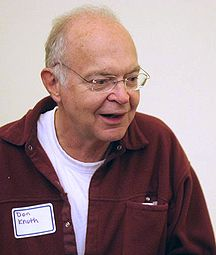
\includegraphics[width=0.5\linewidth]{knuth1} \\ а)}
  \end{minipage}
  \hfill
  \begin{minipage}[h]{0.49\linewidth}
    \center{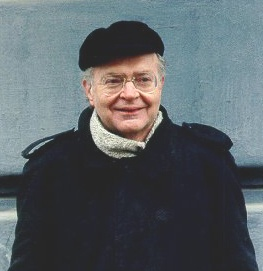
\includegraphics[width=0.5\linewidth]{knuth2} \\ б)}
  \end{minipage}
  \caption{Очень длинная подпись к изображению, на котором представлены две фотографии Дональда Кнута}
  \label{img:knuth}  
\end{figure}

%\newpage
%============================================================================================================================
\section{Пример вёрстки списоков} \label{sect2_3}

\noindent Нумерованный список:
\begin{enumerate}
  \item Первый пункт.
  \item Второй пункт.
  \item Третий пункт.
\end{enumerate}

\noindent Маркированный список:
\begin{itemize}
  \item Первый пункт.
  \item Второй пункт.
  \item Третий пункт.
\end{itemize}

\noindent Вложенные списки:
\begin{itemize}
  \item Имеется маркированный список.
  \begin{enumerate}
    \item В нём лежит нумерованный список,
    \item в котором
    \begin{itemize}
      \item лежит ещё один маркированный список.
    \end{itemize}    
  \end{enumerate}
\end{itemize}


\clearpage           % Глава 2
\chapter{Методика работы} \label{chapt3}

\section{Критерии отбора данных и подготовка данных к физическому анализу} \label{sect3_cuts}
В данной работе были использованы данные, полученные экспериментом PHENIX, в столкновениях $p+p$ (2005 год набора данных), Cu+Au и U+U (2012 г), \heau \ (2014г) и $p$+Al (2015 г).


\begin{table}
	\caption{Критерии отбора данных}
	\centerfloat{\begin{tabular}{|c|c|}
			\hline
			 
			%Показатель качества треков & $31||63||51$ \\ \hline
			% & $|zed| < $ 75 cm \& $|zed|>$ 4 cm \\ \hline
			
  			Ограничение z-координаты & \multirow{2}{*}{$|z_{vtx}| < $ 30 cm} \\ % \cline{1-1}
  			вершины столкновения    &          \\ \hline
			\multirow{4}{*}{Интервал \pt \ измерения \pipm} & p+Al - 0.5 ГэВ/с $< p_T < $ 2.0 ГэВ/с \\
			& \heau - 0.5 ГэВ/с $< p_T < $ 2.0 ГэВ/с  \\ 
			& \cuau - 0.5 ГэВ/с $< p_T < $ 2.0 ГэВ/с  \\ 
			& \uu - 0.5 ГэВ/с $< p_T < $ 2.0 ГэВ/с  \\ \hline
			\multirow{4}{*}{Интервал \pt \ измерения \Kpm} & p+Al - 0.5 ГэВ/с $< p_T < $ 2.0 ГэВ/с \\
			& \heau - 0.5 ГэВ/с $< p_T < $ 2.0 ГэВ/с  \\ 
			& \cuau - 0.5 ГэВ/с $< p_T < $ 2.0 ГэВ/с  \\ 
			& \uu - 0.5 ГэВ/с $< p_T < $ 2.0 ГэВ/с  \\ \hline
			\multirow{4}{*}{Интервал \pt  \ измерения \prot \ и \aprot} & p+Al - 0.5 ГэВ/с $< p_T < $ 2.0 ГэВ/с \\
			& \heau - 0.5 ГэВ/с $< p_T < $ 2.0 ГэВ/с  \\ 
			& \cuau - 0.5 ГэВ/с $< p_T < $ 2.0 ГэВ/с  \\ 
			& \uu - 0.5 ГэВ/с $< p_T < $ 2.0 ГэВ/с  \\ \hline
			
			
	\end{tabular}}
	\label{table:cuts}
\end{table}

Критерии отбора данных, использованные в анализе, приведены в таблице \ref{table:cuts}. Большинство приведенных критериев являются общепринятыми в эксперименте PHENIX. Так общепринятыми являются  выбор событий с минимальным отбором, ограничения z-координаты вершины столкновения и выбор бита качества отслеживания. Также в данной работе были использованы специфические критерии отбора данных -  критерии идентификации заряженных частиц с использованием дрейфовой камеры и времяпролетных детекторов. Критерии идентификации заряженных частиц рассмотрены в разделе \ref{sect3_PID}.

Приведенные критерии отбора данных были также использованы при Монте-Карло моделировании, которое проводилось для оценки эффективности регистрации частиц (п. \ref{sect3:EffRec}) и коррекции, учитывающей увеличение выхода протонов и антипротонов в результате распада частиц (п. \ref{sect3:FeedDown}). 

\subsection{Триггер минимального отбора}
В качестве основного набора данных в эксперименте PHENIX используется набор данных с минимальным отбором <<Minimum Bias>> (MB), который формируется с помощью триггера минимального отбора (MB-триггера).
MB-триггер отбирает события, в которых происходит одновременное срабатывание двух или более ФЭУ из состава BBC счетчиков, расположенных в северном плече эксперимента PHENIX (передняя область быстрот) и южном плече эксперимента PHENIX (задняя область быстрот).
Также события минимального отбора должны удовлетворять условию на ограничение $z$-координаты вершины столкновения $|z| < $30 см. Отбор данных событий осуществляется онлайн с помощью триггера BBC Level-1 (LVL1 триггер).

Эффективность MB-триггера определяется с помощью Монте-Карло моделирования BBC. Отклик ФЭУ и логика платы BBLL1 настраиваются при моделировании в соответствии с условиями эксперимента. Эффективность триггера для неупругих столкновений A+B составляет 92 ± 2\%. 

Поскольку MB-триггер расположен вблизи оси пучка, эффективность регистрации дифракционных событий оказывается выше, чем недифракционных, поскольку для дифракционных событий характерны большие множественности рождения частиц в диапазонах по быстроте $3 <|y|<4$, в то время как недифракционные события характеризуются рождением частиц преимущественно в области малых выстрот $|y|<0.35$. Зависимость эффективности MB-триггера от множественности события в области больших быстрот корректируется с помощью Байес-фактора ($f_{Bias}$). 
Значения поправок $f_{Bias}$ были оценены с помощью моделирования МК Глаубера и представлены в табл. \ref{table:fBias}.

\begin{table}[]
	\caption{Значения $f_{Bias}$, вычисленные с помощью модели Глаубера для различных центральностей \pal \ и \heau \ столкновений.}
	\label{table:fBias}
	
	\begin{tabularx}{\linewidth}
		{
			| >{\centering\arraybackslash}X
			| >{\centering\arraybackslash}X
			| >{\centering\arraybackslash}X | }
		\hline
		Система столкновения & Центральность &  $f_{bias}$  \\ \hline
		\pal & 0-72\%     & 0.80$\pm$0.02       \\
		& 0-20\%     & 0.81$\pm$0.01       \\
		& 20-40\%    & 0.90$\pm$0.02       \\
		& 40-72\%    & 1.05$\pm$0.04    \\ \hline
		
		\heau & 0-88\%     & 0.89$\pm$0.01  \\
		& 0-20\%     & 0.95$\pm$0.01  \\
		& 20-40\%    & 1.01$\pm$0.01  \\
		& 40-60\%    & 1.02$\pm$0.01   \\
		& 60-88\%    & 1.03$\pm$0.05   \\ \hline
		
	\end{tabularx}
\end{table}

\subsection{Определение центральности} \label{sect3:centr}
Центральность является характеристикой столкновения, показывающей степень перекрытия ядер, и непосредственно связанна с прицельным параметром. Лобовым столкновениям с прицельным параметром равным нулю, в которых степень перекрытия ядер максимальна, соответствует значение центральности 0\%. Переферическим столкновениям, в которых ядра проходят по касательной, а прицельный параметр равен сумме радиусов сталкивающихся ядер, соответствует значение центральности 100 \%. В остальных случаях значения центральности варьируются от 0\% до 100 \%, характеризуя степень перекрытия ядер.


\begin{figure}[] 
	\centerfloat
	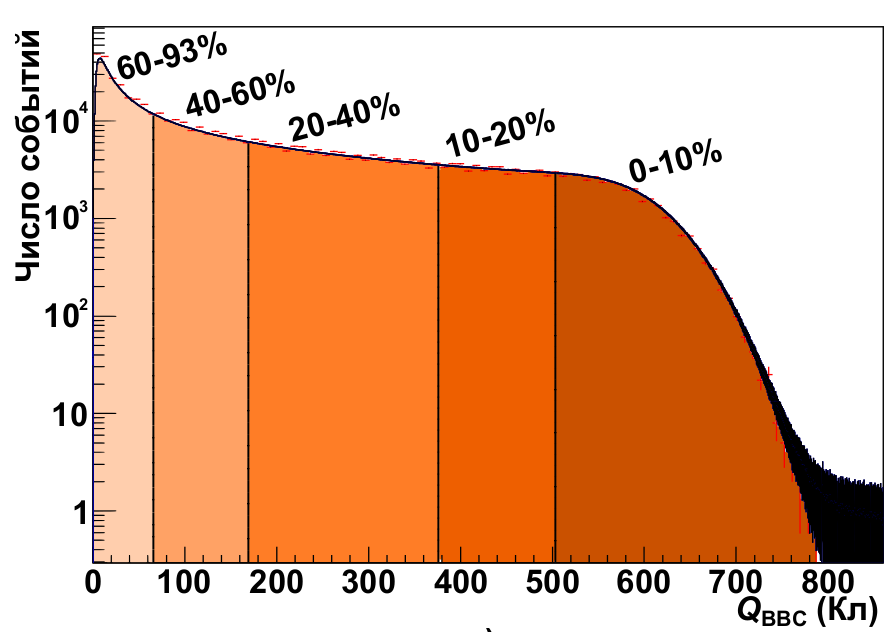
\includegraphics [width=0.7\linewidth]{Methodology/centrality.png}
	\caption{Распределение событий Cu+Au столкновений по величине заряда, зарегистрированного в счетчиках BBC} 
	\label{img:Met_centr}
\end{figure}

Центральность столкновения в эксперименте PHENIX определяется с помощью BBС детектора, который измеряет количество заряженных частиц в переднем и заднем диапазоне быстрот ($3<|\eta|<4$). 
Для определения центральности заполняется гистограмма распределения событий ядро-ядерных столкновений по величине заряда, зарегистрированного в BBC счетчике. Пример данной гистограммы для Cu+Au столкновений приведен на рис. \ref{img:Met_centr}. Далее полученная гистограмма разбивается на части, количество событий в которых пропорционально рассматриваемым интервалам центральности. Разбиение, соответствующее интервалам центральности 0–20 \%, 20–40 \%, 40–60 \%, 60–82 \% обозначено на графике линиями. Интервал центральности 60-92 \% используется как самый переферийный в связи с низкой статистикой в переферических столкновениях.



\begin{table}[]
	\caption{Значения \Ncoll \ и \Npart, вычисленные с помощью модели Глаубера для различных центральностей \pal, \heau, \cuau \ и \uu \ столкновений.}
	\label{table:NcollNpart}
	
	\begin{tabularx}{\linewidth}
		{
			| >{\centering\arraybackslash}X
			| >{\centering\arraybackslash}X
			| >{\centering\arraybackslash}X | }
		\hline
			Центральность & \Ncoll    &  \Npart       \\ \hline \hline
			        &       \bfseries{\pal}   &               \\  \hline
			0-72\%     & 2.1$\pm$0.2    & 3.1$\pm$0.1    \\  \hline
			0-20\%     & 3.4$\pm$0.3    & 4.4$\pm$0.3    \\ \hline
			20-40\%    & 2.3$\pm$0.2    & 3.3$\pm$0.1    \\ \hline
			40-72\%    & 1.7$\pm$0.1   & 1.6$\pm$0.2  \\ \hline \hline
			      &     \bfseries{\heau}      &             \\ \hline
			0-88\%     & 10.4$\pm$0.7 & 11.3$\pm$0.5    \\  \hline
			0-20\%     & 22.3$\pm$1.7 & 21.1$\pm$1.3    \\ \hline
			20-40\%    & 14.8$\pm$1.1 & 15.4$\pm$0.9    \\ \hline
			40-60\%    & 8.4$\pm$0.6  & 9.5$\pm$0.6     \\ \hline
			0-88\%    & 3.4$\pm$0.3  & 4.8$\pm$0.3     \\  \hline \hline
			       &     \bfseries{\cuau}      &             \\  \hline
			0-80\%     & 123.8$\pm$12.0  & 70.4$\pm$3.0    \\  \hline
			0-20\%     & 313.8$\pm$28.4  & 154.8$\pm$4.1     \\  \hline
			20-40\%    & 129.3$\pm$12.4  & 80.4$\pm$3.3     \\  \hline
			40-60\%    & 41.8$\pm$5.3    & 34.9$\pm$2.9   \\ \hline
			60-80\%    & 10.1$\pm$2.0    & 11.5$\pm$1.8   \\ \hline \hline
			       &     \bfseries{\uu}     &            \\ \hline
			0-20\%     & 935$\pm$98    & 330$\pm$6   \\ \hline
			20-40\%    & 335$\pm$33    & 259$\pm$7   \\ \hline
			40-60\%    & 81$\pm$13     & 65$\pm$6    \\ \hline
			60-80\%    & 17$\pm$4  & 18$\pm$3   \\
				\hline
	
	\end{tabularx}
\end{table}

Центральность столкновения связана с величинами $N_{part}$ и $N_{coll}$ - количеством нуклонов участников и количеством парных нуклон-нуклонных соударений соответственно. Величины $N_{part}$ и $N_{coll}$ были определены с помощью модели Глаубера и представлены в таблице \ref{table:NcollNpart}.

\subsection{Исключение проблемных сегментов} \label{sect3_DM}
За время экусплуатации эксперимента PHENIX некоторые сегменты дрейфовых камер выходят из строя, что приводит к уменьшению уровня загрузки ДК. Области низкой загрузки ДК принято называть <<мертвыми>> областями. 
Для корректной оценки эффективности регистрации заряженных адронов необходимо исключить мертвые области из дальнейшего анализа. 
Исключение мертвых областей проводится с помощью построения гистограмм загрузки ДК, которые представляют собой распределение уровня загрузки дрейфовой камеры в зависимости от азимутального угла $\alpha$ (угла отклонения частицы в магнитном поле) и полярного угла $\varphi$, который для удобства заменяется номером <<платы>>. Номер <<платы>> связан с углом $\varphi$ треков заряженных частиц следующими соотношениями: 

\begin{equation}
	N_{восточное плечо} = \left( \frac{3,72402 - \varphi + 0,008047 \cdot cos(\varphi + 0,87851)}{0,01963496} \right)
\end{equation}


\begin{equation}
	N_{западное плечо} = \left( \frac{0,573231 + \varphi - 0,0046 \cdot cos(\varphi + 0,05721)}{0,01963496} \right)
\end{equation}

Полученные гистограммы загрузки представлены на рис. \ref{img:Met_DMRun12}-\ref{img:Met_DMRun15}. 
На гистограммах загрузки ДК (панели а), в) на рис. \ref{img:Met_DMRun12}-\ref{img:Met_DMRun15}) присутствуют <<мертвые>> области, уровень загрузки в которых значительно ниже среднего камере. 
%Такие области дрейфовых камер с пониженной загрузкой  принято называть <<мертвыми>> областями. 
%Для уменьшения искажений мертвые области исключаются из анализа.
Панели б), г) на рис \ref{img:Met_DMRun12}-\ref{img:Met_DMRun15} представляют гистограмму загрузки ДК после исключения мертвых областей. 
Совокупность мертвых областей, исключаемых из анализа, называется мертвой картой дрейфовой камеры. Мертвые карты также были применены при проведении моделирования (см. раздел \label{sect3:EffRec}).


\begin{figure}[] 
	\centerfloat
	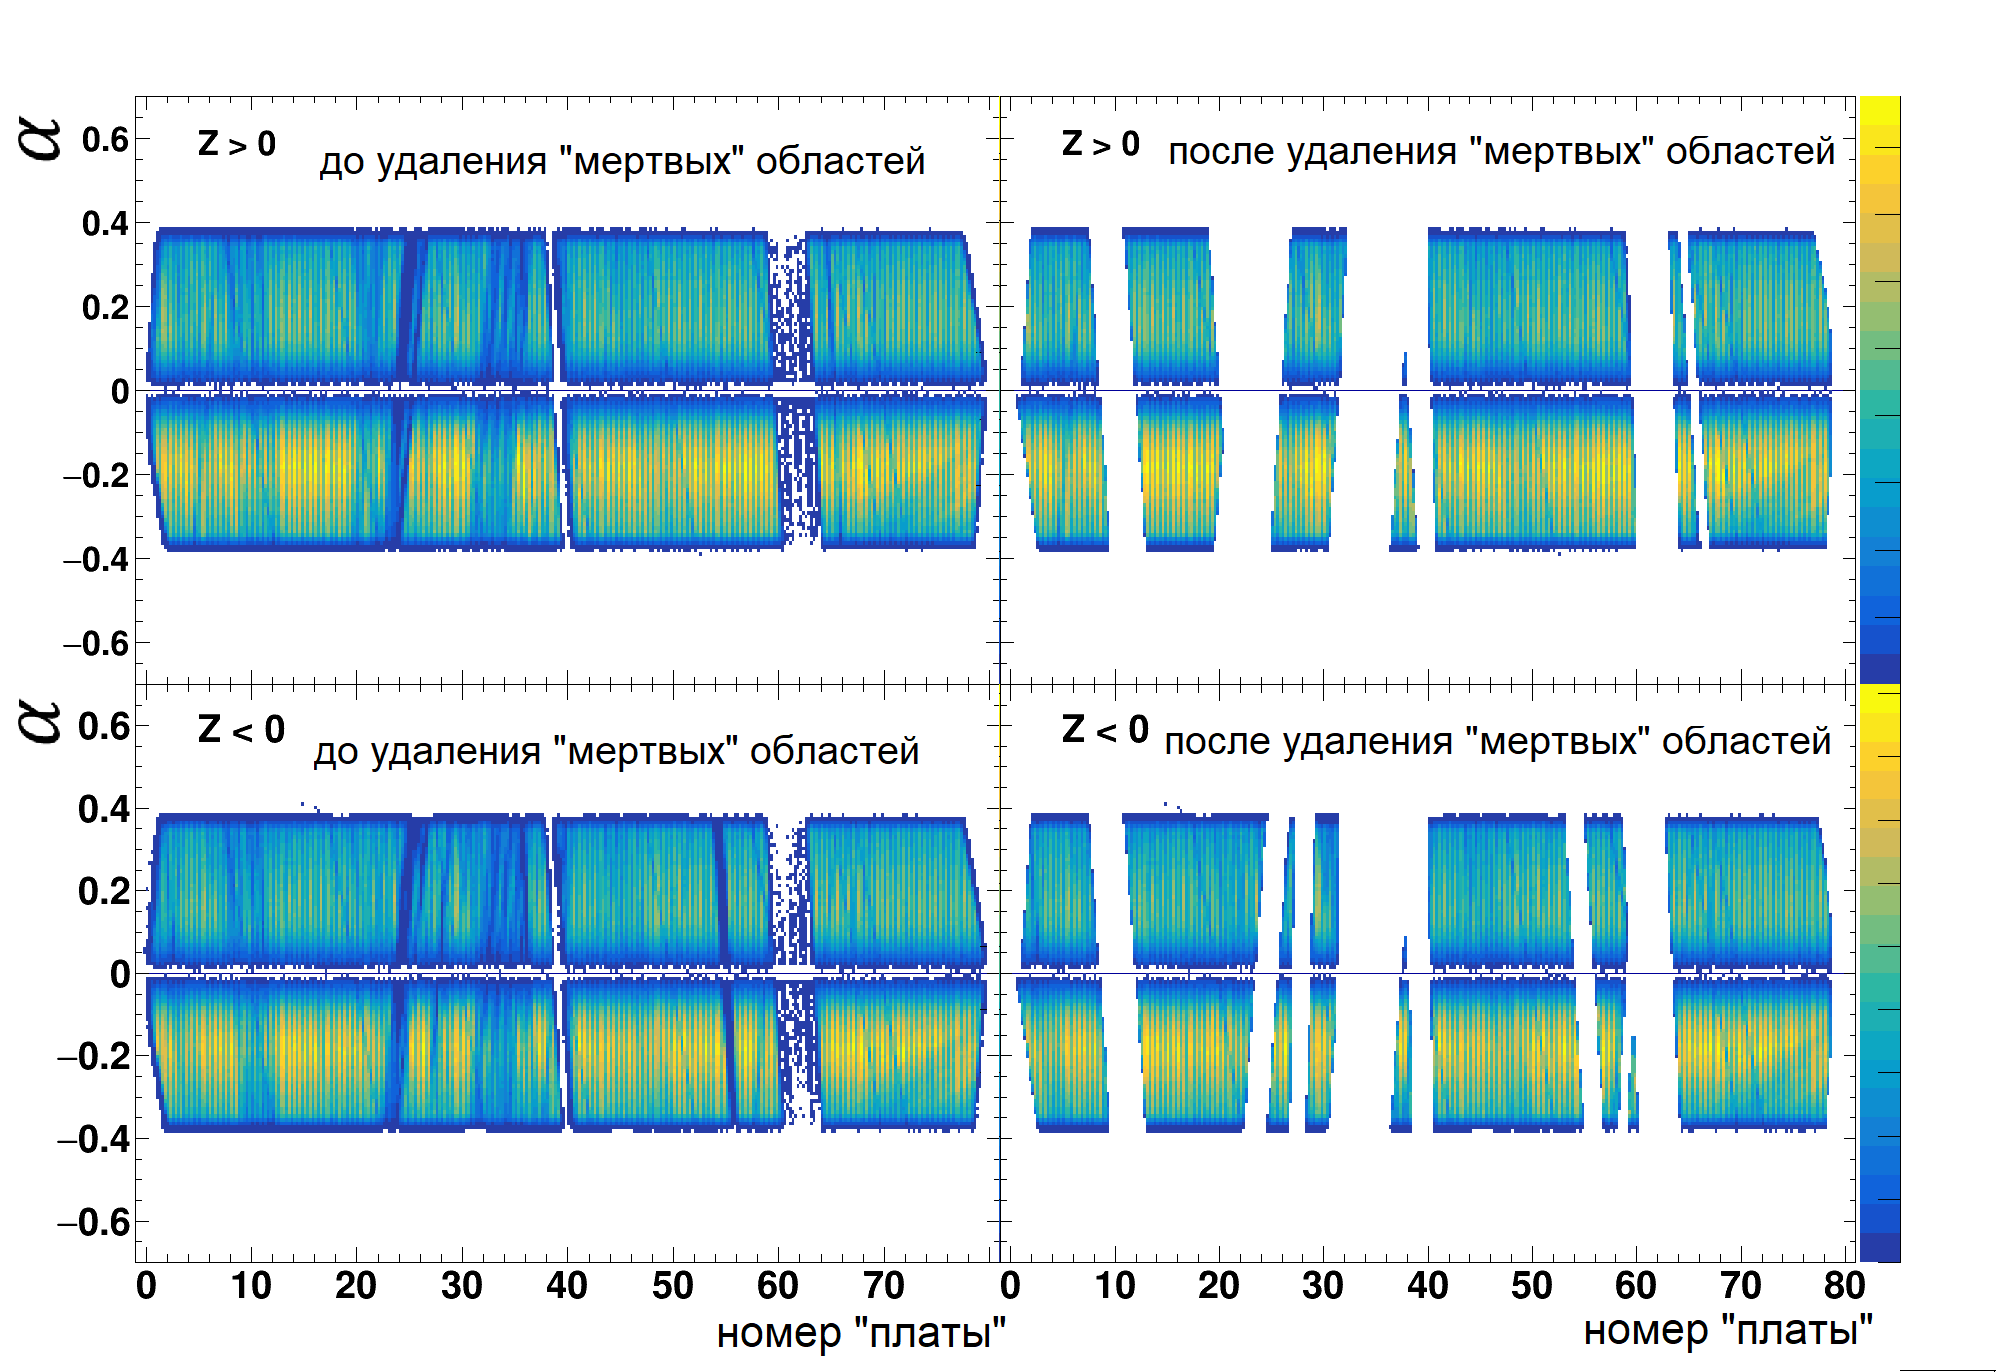
\includegraphics [width=0.8\linewidth]{Methodology/DC_DM_HeAu.png}
	\caption{Гистограмма загрузки дрейфовых камер в 2012 году} 
	\label{img:Met_DMRun12}
\end{figure}

\begin{figure}[] 
	\centerfloat
	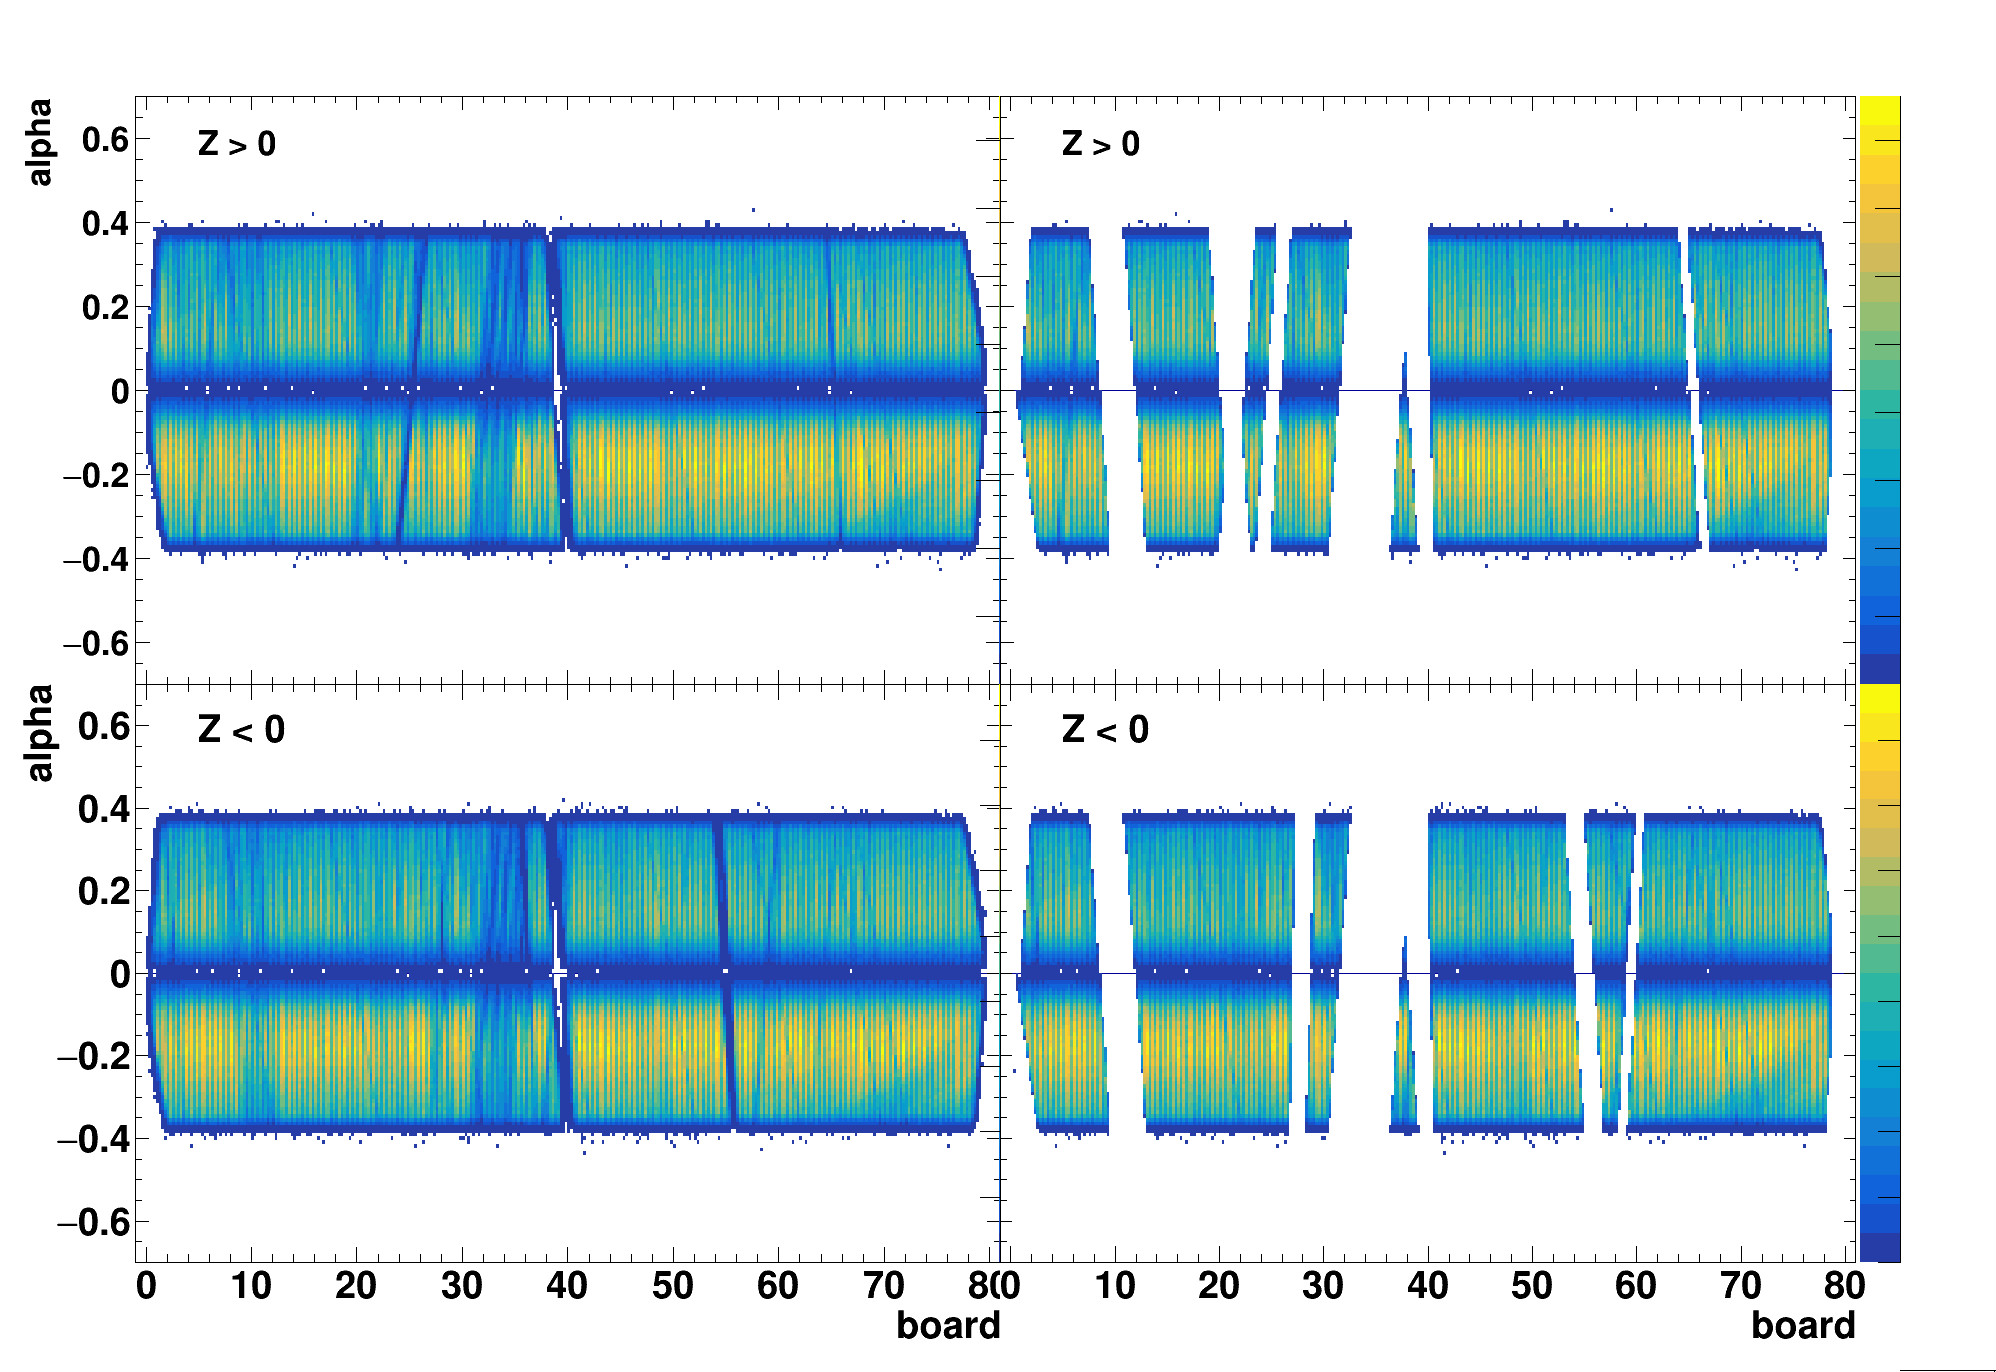
\includegraphics [width=0.8\linewidth]{Methodology/DC_DM_CuAu.png}
	\caption{Гистограмма загрузки дрейфовых камер в 2014 году} 
	\label{img:Met_DMRun14}
\end{figure}

\begin{figure}[] 
	\centerfloat
	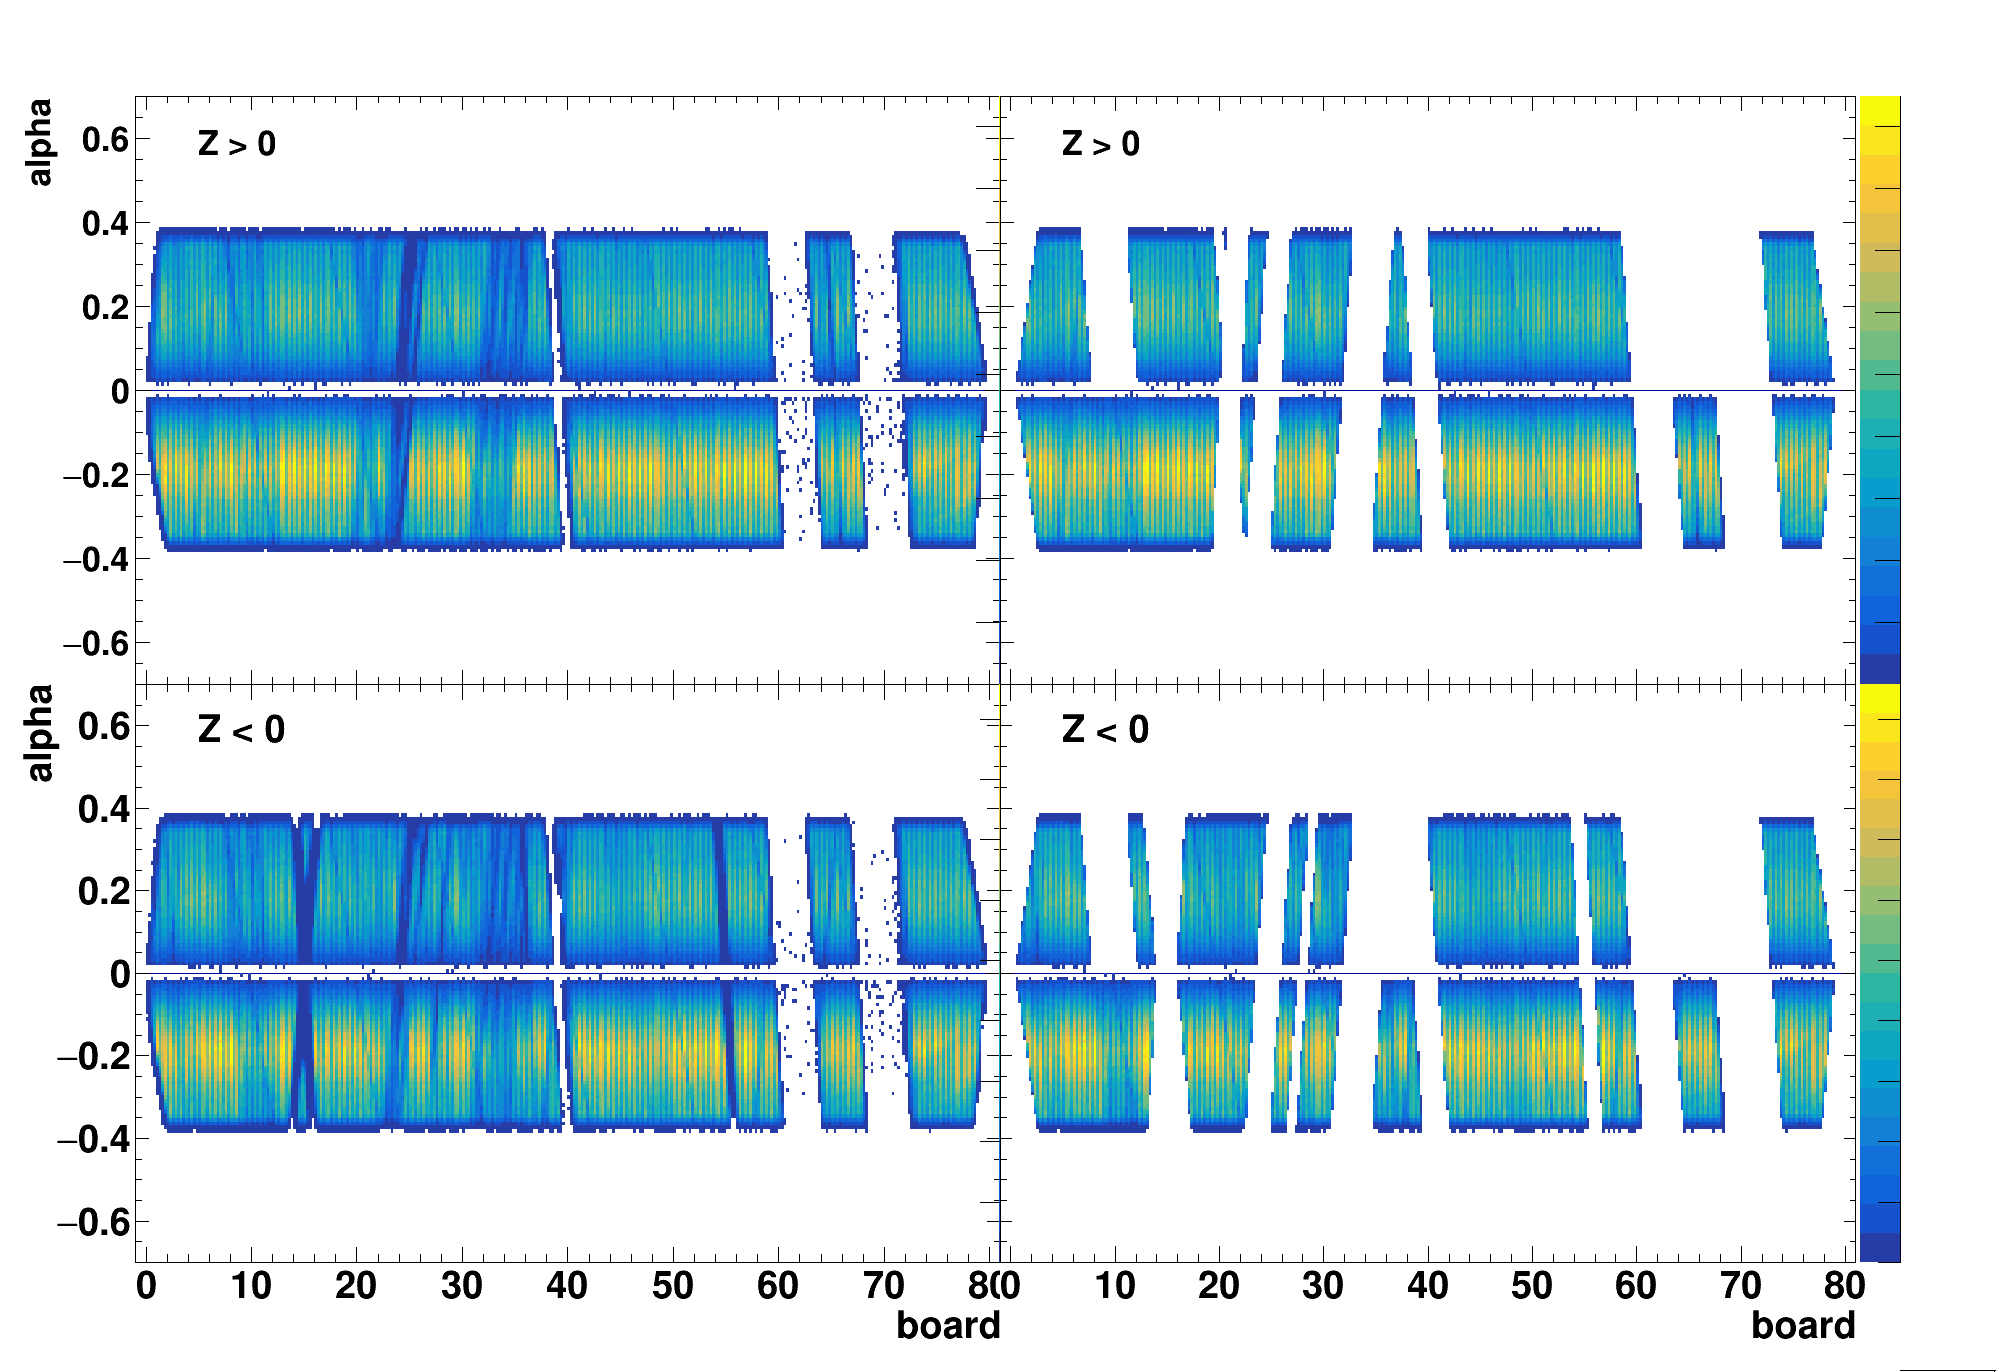
\includegraphics [width=0.8\linewidth]{Methodology/DC_DM_pAl.png}
	\caption{Гистограмма загрузки дрейфовых камер в 2015 году} 
	\label{img:Met_DMRun15}
\end{figure}


\subsection{Измерение первичного выхода заряженных адронов} \label{sect3_PID}
Заряженные адроны регистрируются непосредственно с помощью времяпролетной и дрейфовых камер эксперимента PHENIX. Квадрат массы частиц, зарегистрированных во времяпролетной и дрейфовой камерах, может быть определен в соответствии с выражением \ref{eq:TOFm2}:
\begin{equation}
	\label{eq:TOFm2}
	m^2 = \frac{p^2}{c^2} \left(\frac{t^2 c^2}{L^2} - 1 \right)
\end{equation}
где $p$ - импульс частицы, измеренный с помощью дрейфовой камеры, $L$ - длина, пройденная частицей в сцинтилляторной планке TOF, $c$ - скорость света. 
На рис. \ref{img:TOF_PID}а представлено распределение произведения квадрата массы и заряда регистрируемых адронов в зависимости от поперечного импульсаб полученное в соответствии с выражением \ref{eq:TOFm2}.


\begin{table}[]
	\caption{\pt-интервалы измерений заряженных адронов в \pal, \heau, Cu+Au и U+U системах столкновений.}
	\label{table:pt_ranges}
	
	\begin{tabularx}{\linewidth}
		{
			| >{\centering\arraybackslash}X
			| >{\centering\arraybackslash}X
			| >{\centering\arraybackslash}X
			| >{\centering\arraybackslash}X
			| >{\centering\arraybackslash}X | }
		\hline
	\pt (GeV/c) &  \pal & \heau  & Cu+Au & U+U  \\ \hline
	\pip  & 0.5 - 2.0  &  0.5 - 3.0  &  0.5 - 3.0  & 0.5 - 3.5  \\
	\pim  & 0.5 - 2.0  &  0.5 - 2.0  &  0.5 - 3.0  & 0.5 - 3.0  \\
	\Kp   & 0.5 - 1.8  &  0.5 - 2.0  &  0.5 - 2.0  & 0.5 - 2.0  \\
	\Km   & 0.5 - 1.8  &  0.5 - 2.0  &  0.5 - 2.0  & 0.5 - 2.0  \\
	\prot &  &  0.5 - 4.0  &  0.5 - 4.0  &    0.5 - 4.0     \\
	\aprot & 0.5 - 2.5  &  0.5 - 4.0  &  0.5 - 4.0  &  0.5 - 4.0 \\ \hline
		
	\end{tabularx}
\end{table}

% Сигналы, соответствующие протонам, каонам и пионам, на данном распределении хорошо различимы.

Для идентификации типа частиц, сигналы, зарегистрированные в TOF, аппроксимируются функциями Гаусса с среднеквадратичными отклонениями ($\sigma_{TOF}$) и математическими ожиданиями ($m_{TOF}^2$) в каждом интервале $\Delta p_T = 0.5$ GeV/c диапазона \pt \ идентификации адронов. Диапазоны идентификации адронов по \pt \ приведены в табл.~\ref{table:pt_ranges}.  Пример аппроксимации в диапазоне поперечных импульсов 1.0-1.1 ГэВ/с представлен на рис. \ref{img:TOF_PID}. Далее для каждого типа адрона $h$ ($h = \pi^{\pm}$, $K^{\pm}$, $p$, $\bar{p}$) полученные дискретные зависимости $\sigma_{TOF_{h}}(p_T)$ и $m_{TOF_{h}}^2(p_T)$ параметризуются уравнением ~\ref{eq:TOFgaus_approx}. 
\begin{equation}
	m_{TOF_{h}}^2(p_T),\sigma_{TOF_{h}}(p_T) = p_0 +\frac{p_1}{p_T} + \frac{p_2}{p_T^2} + p_3 \cdot e^{\sqrt{p_T}} +p_4 \cdot \sqrt{p_T},
	\label{eq:TOFgaus_approx}
\end{equation}

Значения $\sigma_{TOF_{h}}$ и $m_{TOF_{h}}^2$, вычисленные по формуле \ref{eq:TOFgaus_approx}, используются для идентификации частиц. Частица с зарегистрированным квадратом массы $m_{TOF}^2$ идентифицируется как адрон $h$ в том случае, если  $m_{TOF}^2$ удовлетворяет неравенствам 
$$ m_{TOF_{h}}^2 -2\sigma_{TOF_{h}} < m_{TOF}^2 < m_{TOF_{h}}^2 +2\sigma_{TOF_{h}}. $$
При значениях поперечных импульсов \pt$\sim$2-3 ГэВ/$с$ происходит наложение сигналов заряженных адронов. В связи с этим было введено дополнительное условие, обеспечивающее непопадание массы частицы в диапазон $\pm 2\sigma_{TOF_{h}}$ соседних сигналов частиц.
Условия идентификации заряженных адронов приведены в таблице \ref{table:m2cuts}.


\begin{comment}
Диапазон поперечных импульсов разбивается на промежутки шириной 0.1 ГэВ/с, на каждом из которых сигналы заряженных адронов аппроксимируются функцией Гаусса. Пример такой аппроксимации в диапазоне поперечных импульсов 1.0-1.1 ГэВ/с представлен на рис. \ref{img:TOF_PID}. 
Далее зависимости от поперечного импульса полученных среднеквадратичных отклонений ($\Tilde{\sigma}_h$) и математических ожиданий ($\Tilde{m}^2_h$) функций Гаусса для адронов h (h=\pipm,\Kpm,\prot, \aprot ) аппроксимировались функцией  \ref{eq:TOFgaus_approx}.

\begin{equation}
	\label{eq:TOFgaus_approx}
	f(p_T) = P_0 +P_1/p_T + P_2/p_T^2 + P_3 \cdot exp(\sqrt{p_T}) +P_4 \cdot \sqrt{p_T} 
\end{equation}
где $P_i, i \in [1,4]$ - параметры аппроксимации.

Значения $\sigma_h$ и $m_h$, вычисленные по формуле \ref{eq:TOFgaus_approx}, использовались для идентификации частиц. Частица, с зарегистрированным квадратом массы $m^2$, идентифицируется как адрон h в том случае, если  $m^2$ удовлетворяет неравенствам $$ m^2_h -2\sigma_h < m^2 < m^2_h +2\sigma_h. $$
При значениях поперечных импульсов \pt~2-3 ГэВ/с происходит наложение сигналов заряженных адронов. В связи с этим было введено дополнительное условие, обеспечивающее непопадание массы частицы в диапазон $\pm 2\sigma_h$ соседних сигналов частиц.
Условия идентификации заряженных адронов приведены в таблице \ref{table:m2cuts}.
\end{comment}

\begin{table}[]
	\caption{Условия идентификации частиц}
	\label{table:m2cuts}
	\begin{center}
		\begin{tabular}{|c|c|}
			\hline
			\multirow{2}{*}{\pipm} & $|m^2_{TOF} - m^2_{TOF_{\pi}}|<2\sigma_{TOF_{\pi}}$ \\ 
			& $m^2_{TOF} < m^2_{TOF_{K}}-2\sigma_{TOF_{K}}$ \\ \hline
			\multirow{3}{*}{\Kpm}  & $|m^2 - m^2_{TOF_{K}}|<2\sigma_{TOF_{K}}$  \\ 
			& $m^2_{TOF} > m^2_{TOF_{\pi}}+2\sigma_{TOF_{\pi}}$\\  
			& $m^2_{TOF} < m^2_{TOF_{p}}+2\sigma_{TOF_{p}}$ \\ \hline
			\multirow{2}{*}{\prot, \aprot} & $|m^2_{TOF} - m^2_{TOF_{p}}|<2\sigma_{TOF_{p}}$ \\ 
			& $m^2_{TOF} > m^2_{TOF_{K}}+2\sigma_{TOF_{K}}$ \\ \hline
		\end{tabular}
	\end{center}
\end{table}



\begin{figure}[ht] 
	\centerfloat
	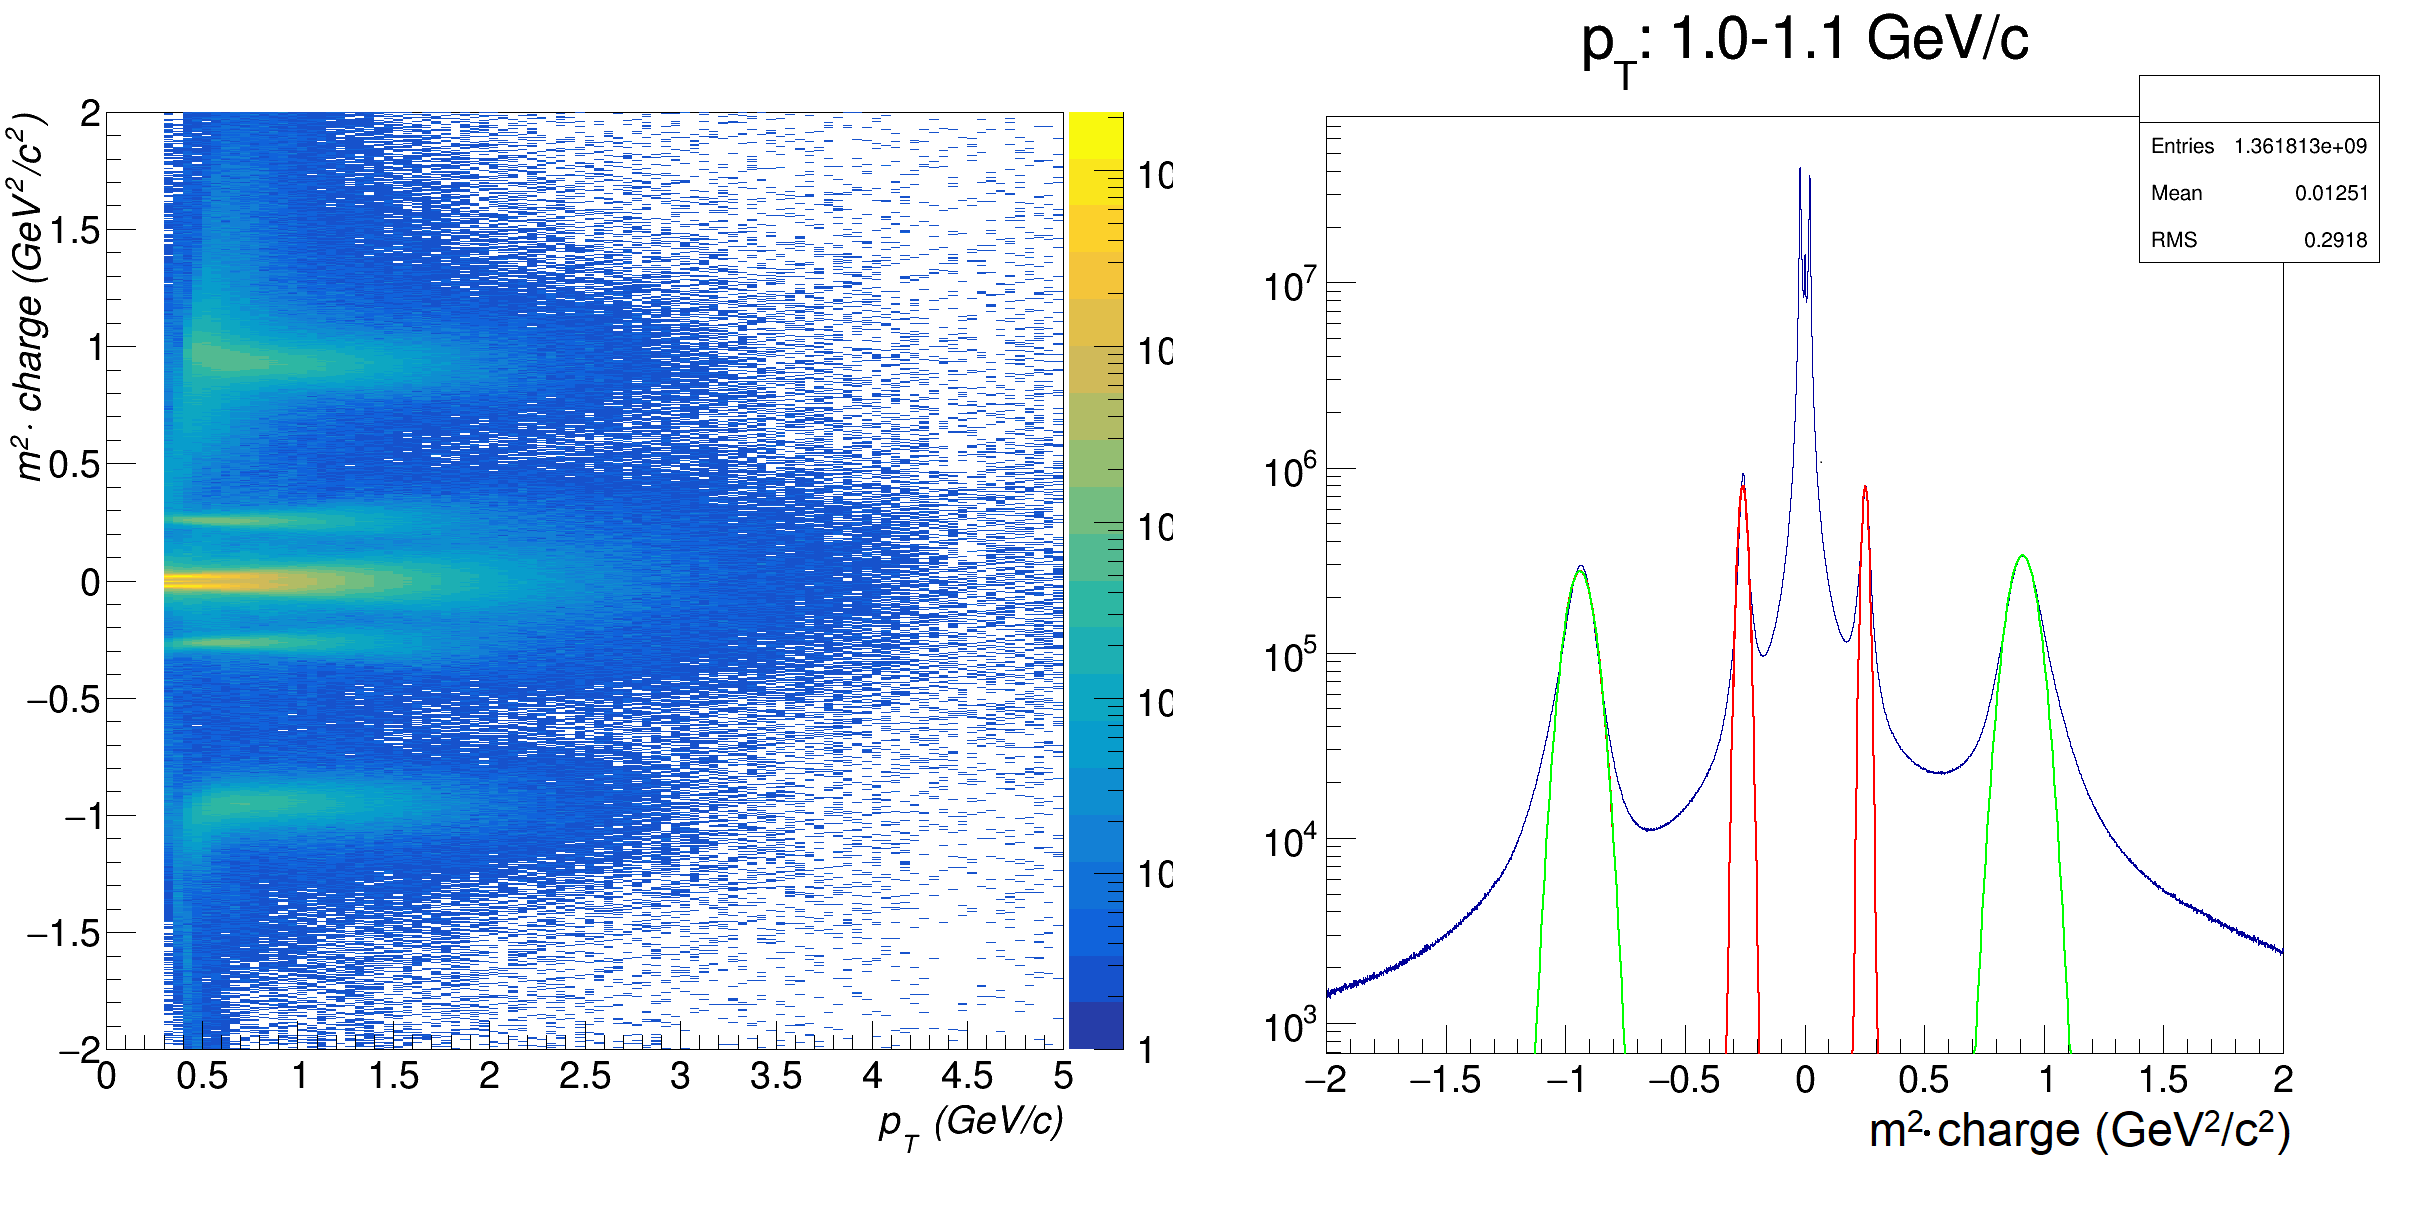
\includegraphics [width = 0.9\linewidth] {Methodology/TOF2.png}
	\caption{а) Двухмерное распределение произведения квадрата массы на заряд регистрируемых адронов в зависимости от поперечного импульса б) Пример аппроксимации сигналов от заряженных адронов функцией Гаусса в диапазоне поперечных импульсов 1.0 -1.1 ГэВ/с} 
	\label{img:TOF_PID}  
\end{figure}

\section{Оценка коррекций измерения первичного выхода заряженных адронов}

\subsection{Оценка эффективности регистрации} \label{sect3:EffRec}

%To correct for geometrical acceptance, analysis cuts, particle interactions with detector materials, and in-flight decays (for pions and kaons), we use single particle Monte Carlo (MC) simulations. For these simulations, single particles are generated using a random generator, with flat distributions in rapidity, azimuth, and \pT. The random particles are then run through a geant simulation of PHENIX to determine the interactions of the single particles with the detector subsystems and support structures. Next, all the detector response information is fed through the usual PHENIX reconstruction software to produce simulated tracks. Finally, these simulated tracks are analyzed in the exact same way as tracks from the real data in order to determine the corrections. The total correction factor, FC(\pT), is given by the following relation:

%\begin{equation}
%  \label{eq:CorrFactor}
%    FC(p_T) = %\frac{dN_{output}/dp_T}{dN_{input}/dp_T} = %\epsilon_{acceptance}\epsilon_{efficiency}\epsilon{cuts}
%\end{equation}
%To correct for the detector occupancy effect, which is most significant in the TOFW, we run embedding simulations, where a track from single particle MC simulations is embedded into a real event, and the occupancy correction is determined from the relative efficiencies of reconstructing the single track in isolation and in the event. This correction is the largest in the most central Au+Au collisions where the multiplicity is the highest and therefore the occupancy effect is the strongest. In the most peripheral Au+Au collisions the multiplicity is low enough that there is essentially no effect. The same is true in d+Au collisions, where no correction is applied.

Для того чтобы оценить количество адронов, родившихся в вершине ядроядерных взаимодействий, измеренные значения первичного выхода адронов должны быть скорректированы на эффективность регистрации ($\epsilon_{reg}$) адронов, учитывающий ограниченный аксептанс времяпролетной камеры, детекторные эффекты (различные шумы, разрешение и калибровка, нелинейность, эффективность триггеров реального времени и т.д.) и используемые при отборе данных ограничения.

Оценка эффективности регистрации частиц была проведена с помощью метода Монте-Карло.
Частицы с заданными массами покоя, координатами вершины рождения, энергией генерируются с помощью генератора  случайных чисел с плоскими распределениями по быстроте, азимуту и поперечному импульсу \pt. Затем сгенерированные частицы поступают в качестве входных данных в программный пакет PISA для определения взаимодействия отдельных частиц с подсистемами детектора PHENIX. 

PISA (PHENIX Integrated Simulation Application) является программой моделирования ядро-ядерных столкновений методом Монте-Карло, разработанного для детектора PHENIX на основе GEANT3.
Программа PISA учитывает геометрию, пространственное расположение и материал изготовления детекторных подсистем спектрометра PHENIX, их пространственные, импульсные и энергетические разрешения, а также конфигурация магнитного поля, полностью соответствующие структуре реальной установки в данном цикле ядро-ядерных столкновений.

%Информация, полученная в результате работы программы GEANT4 обрабатывается с помощью стандартного программного обеспечения эксперимента  PHENIX для реконструкции треков.Наконец, ...
Для обработки данных, полученных в результате моделирования, применяются те же критерии отбора событий и идентификации частиц, что и для экспериментальных данных (\ref{sect3_cuts}).

Функция эффективности регистрации вычисляется согласно следующему соотношению:
$$\epsilon_{reg} = \frac{N_{reg}(p_T)}{N_{tot}(p_T)}$$
где $N_{reg}$ - количество адронов, зарегистрированных в Монте-Карло модели, $N_{tot}$ - общее количество адронов, разыгранное в Монте-Карло модели.

%Входными данными для проекта PISA являются выборки частиц со случайно разыгранными величинами характеристик: координатами вершины рождения, массой покоя, каналом распада, энергией и проекциями импульса, моделирующие спектр частиц, рожденных в процессе ядро-ядерных столкновений. Розыгрыш этих характеристик формируется в соответствии с плоскими распределениями по вершине вдоль оси $z$ поперечному импульсу, псевдобыстроте и азимутальному углу смоделированных частиц. 
В таблице \ref{tab:Met_sim} приведены числа событий и границы изменения величин вершины, поперечного импульса, псевдобыстроты и азимутального угла в смоделированных выборках для исследуемых адронов.

\begin{table}[h]
	\centering
	\caption{Параметры моделирования}
	\begin{tabular}{|c|c|c|c|c|c|c|}
		\hline
		Частица &
		\begin{tabular}[c]{@{}l@{}}Количество\\ событий\end{tabular} & 
		$\Delta$ y& 
		\begin{tabular}[c]{@{}l@{}}$\phi$\\ рад\end{tabular}& \begin{tabular}[c]{@{}l@{}}$p_T^{max}$\\ ГэВ/с\end{tabular} & \begin{tabular}[c]{@{}l@{}}$p_T^{min}$\\ ГэВ/с\end{tabular} & \begin{tabular}[c]{@{}l@{}}Вершина\\см\end{tabular} \\ 
		\hline \pip & $10 \cdot 10^6$ & -0.5 - 0.5 & $\pi/2 - 3\pi/2$ & 0.0 & 3.5 & -30 - 30 \\
		\hline \pim & $10 \cdot 10^6$ & -0.5 - 0.5 & $\pi/2 - 3\pi/2$ & 0.0 & 3.5 & -30 - 30 \\
		\hline \Kp & $10 \cdot 10^6$ & -0.5 - 0.5 & $\pi/2 - 3\pi/2$ & 0.0 & 2 & -30 - 30 \\
		\hline \Km & $10 \cdot 10^6$ & -0.5 - 0.5 & $\pi/2 - 3\pi/2$ & 0.0 & 2 & -30 - 30 \\
		\hline \prot & $10 \cdot 10^6$ & -0.5 - 0.5 & $\pi/2 - 3\pi/2$ & 0.0 & 5 & -30 - 30 \\
		\hline \aprot & $10 \cdot 10^6$ & -0.5 - 0.5 & $\pi/2 - 3\pi/2$ & 0.0 & 5 & -30 - 30 \\
		\hline
	\end{tabular}
	\label{tab:Met_sim}
\end{table}

Перед расчетом эффективности регистрации была выполнена проверка соответствия данных моделирования и экспериментальных данных путем сравнения распределений треков в данных выборках. Гистограмма распределения треков в зависимости от номера <<платы>> ДК, полученная путем моделирования, была нормирована в соответствии с экспериментальными данными. Результаты сравнения распределений треков в ДК представлены на рисунке \ref{img:DC_compar}. Результаты моделирования соответствуют результатам, полученным в эксперименте.

Аналогичная проверка была выполнена для восточного крыла времяпролетной камеры (TOFE). Гистограммы распределения треков на плоскость $z-y$ детектора TOFУ,полученные с использованием экспериментальных данных и данных моделированияпредставлены на рис. \ref{img:TOFproj_pAl}-\ref{img:TOFproj_CuAu}. Проекции двухмерных гистграмм \ref{img:TOFproj_pAl}-\ref{img:TOFproj_CuAu} на оси $y$ и $z$ представлены на верхней и нижней панелях соответсвенно на рис. \ref{img:TOFproj_pAl}-\ref{img:TOFproj_CuAu}.  Результаты моделирования также соответствуют результатам, полученным в эксперименте.

\begin{figure}[] 
	\centerfloat
	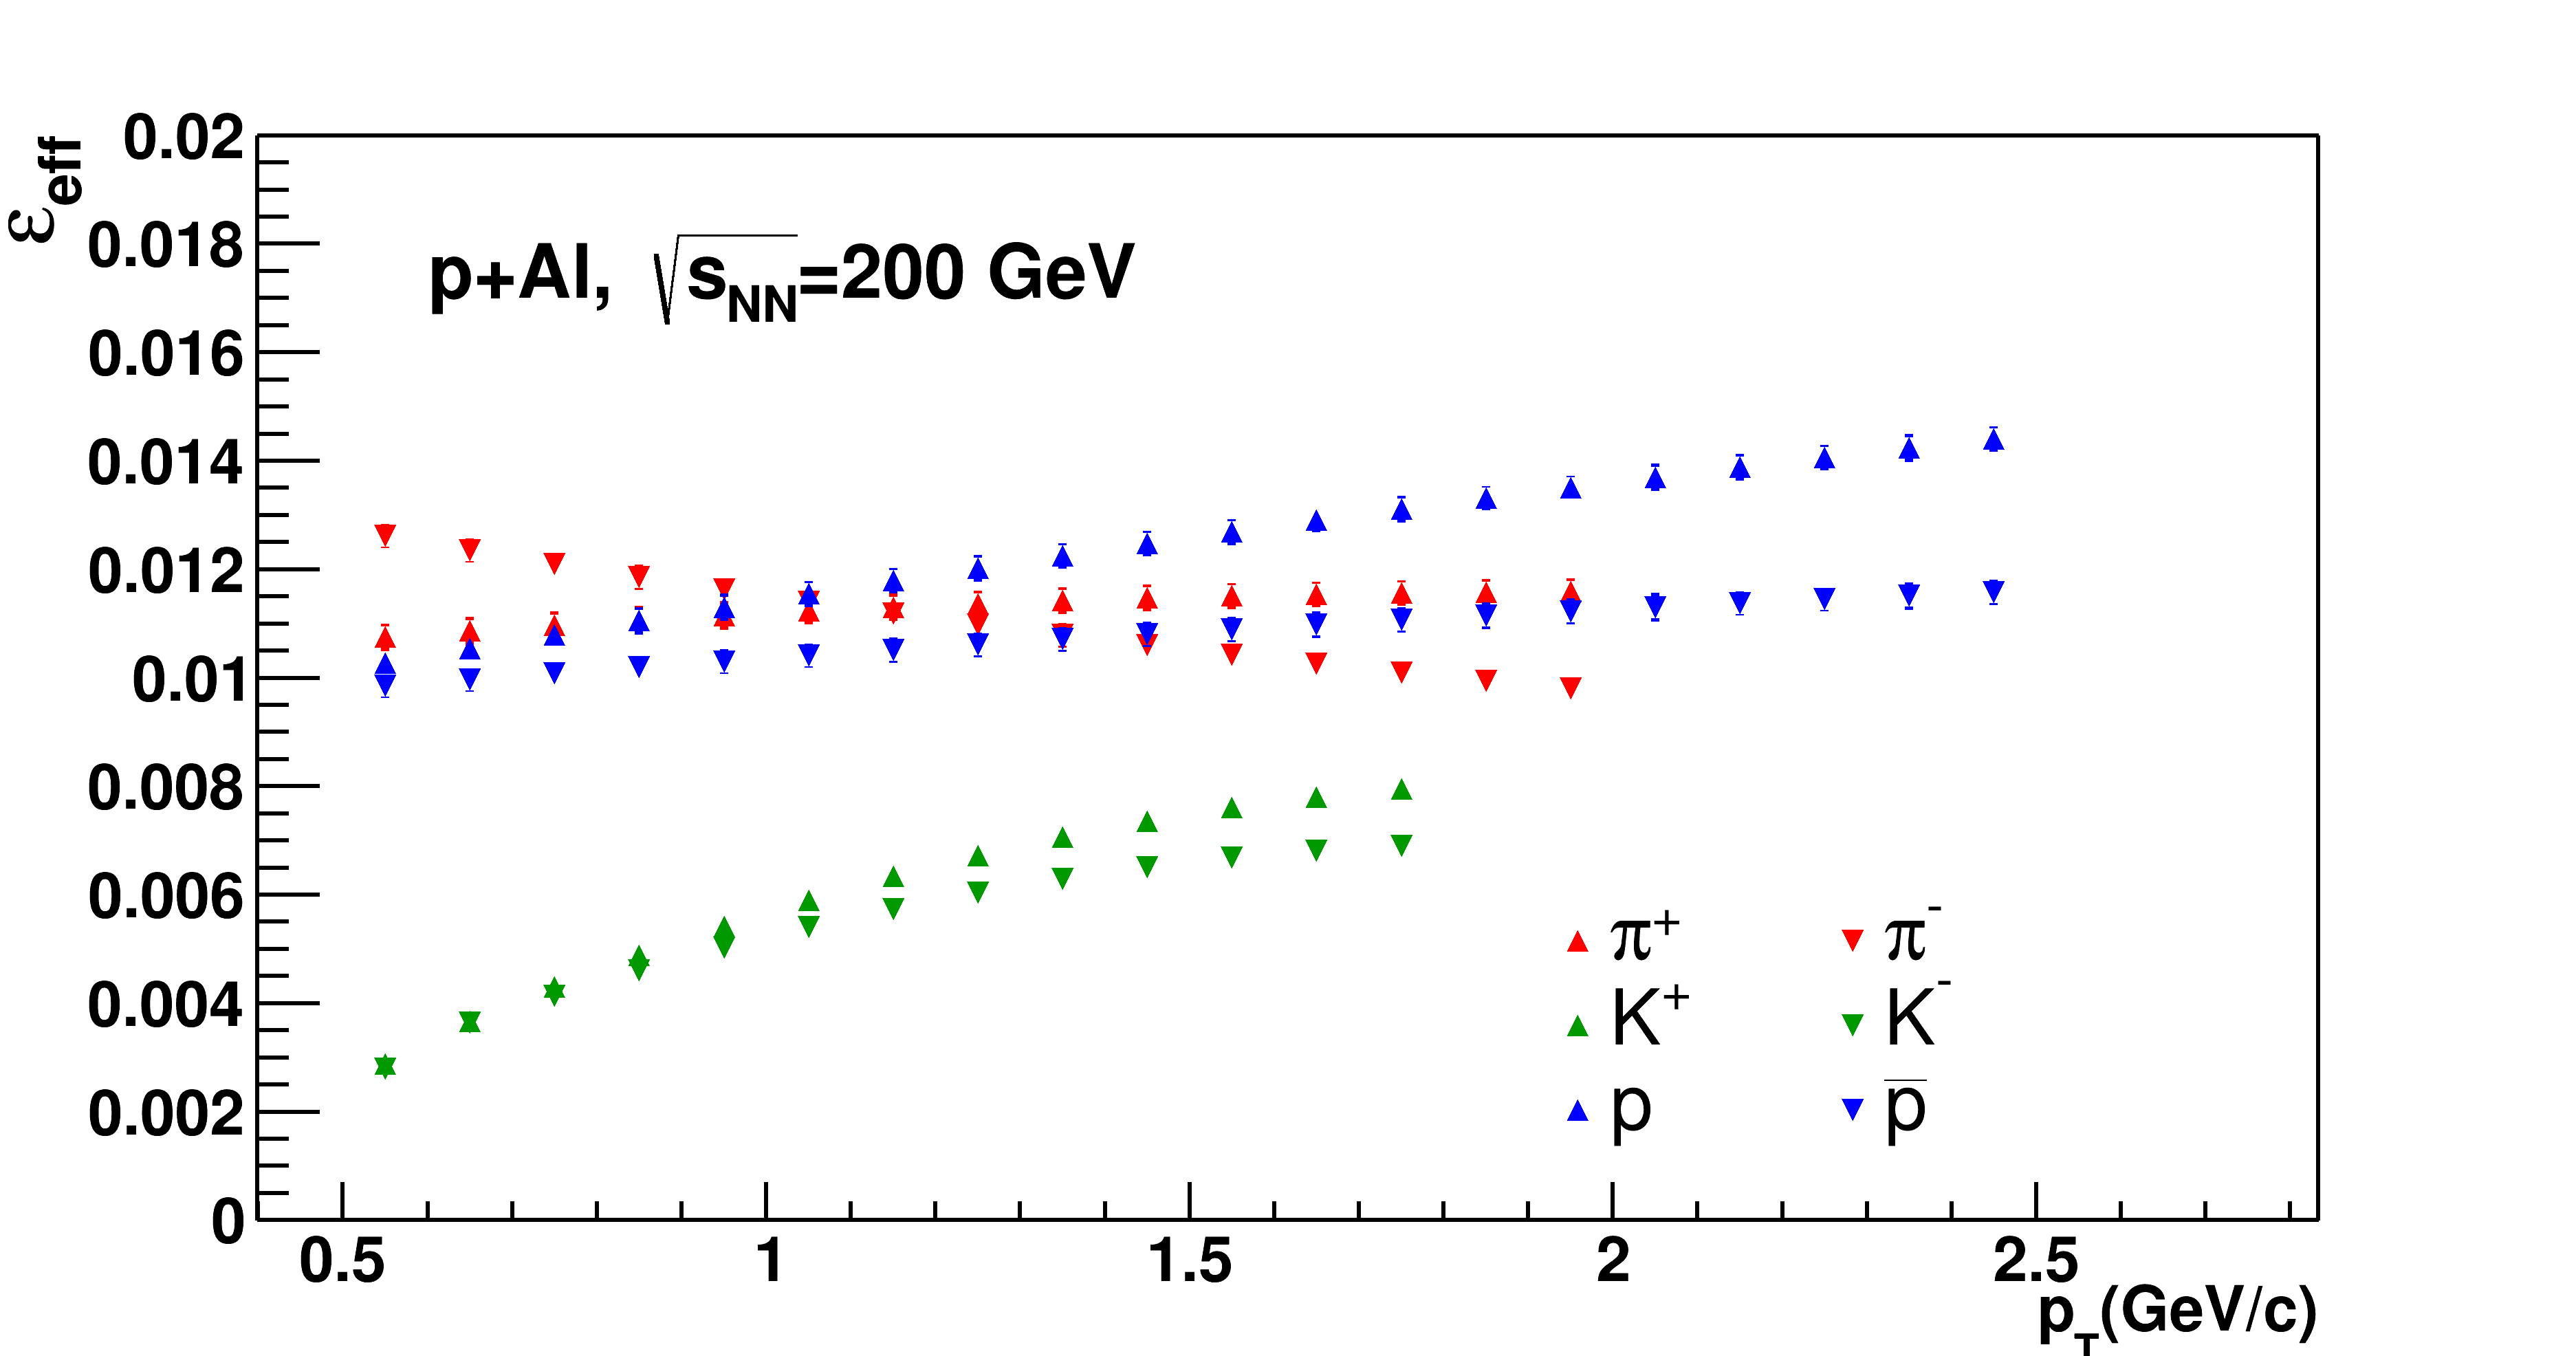
\includegraphics [width=0.9\linewidth]{Methodology/eff_hadron_pAl.png}
	\caption{Эффективность регистрации заряженных адронов в столкновениях \pal.} 
	\label{img:eff_pAl}
\end{figure}

\begin{figure}[] 
	\centerfloat
	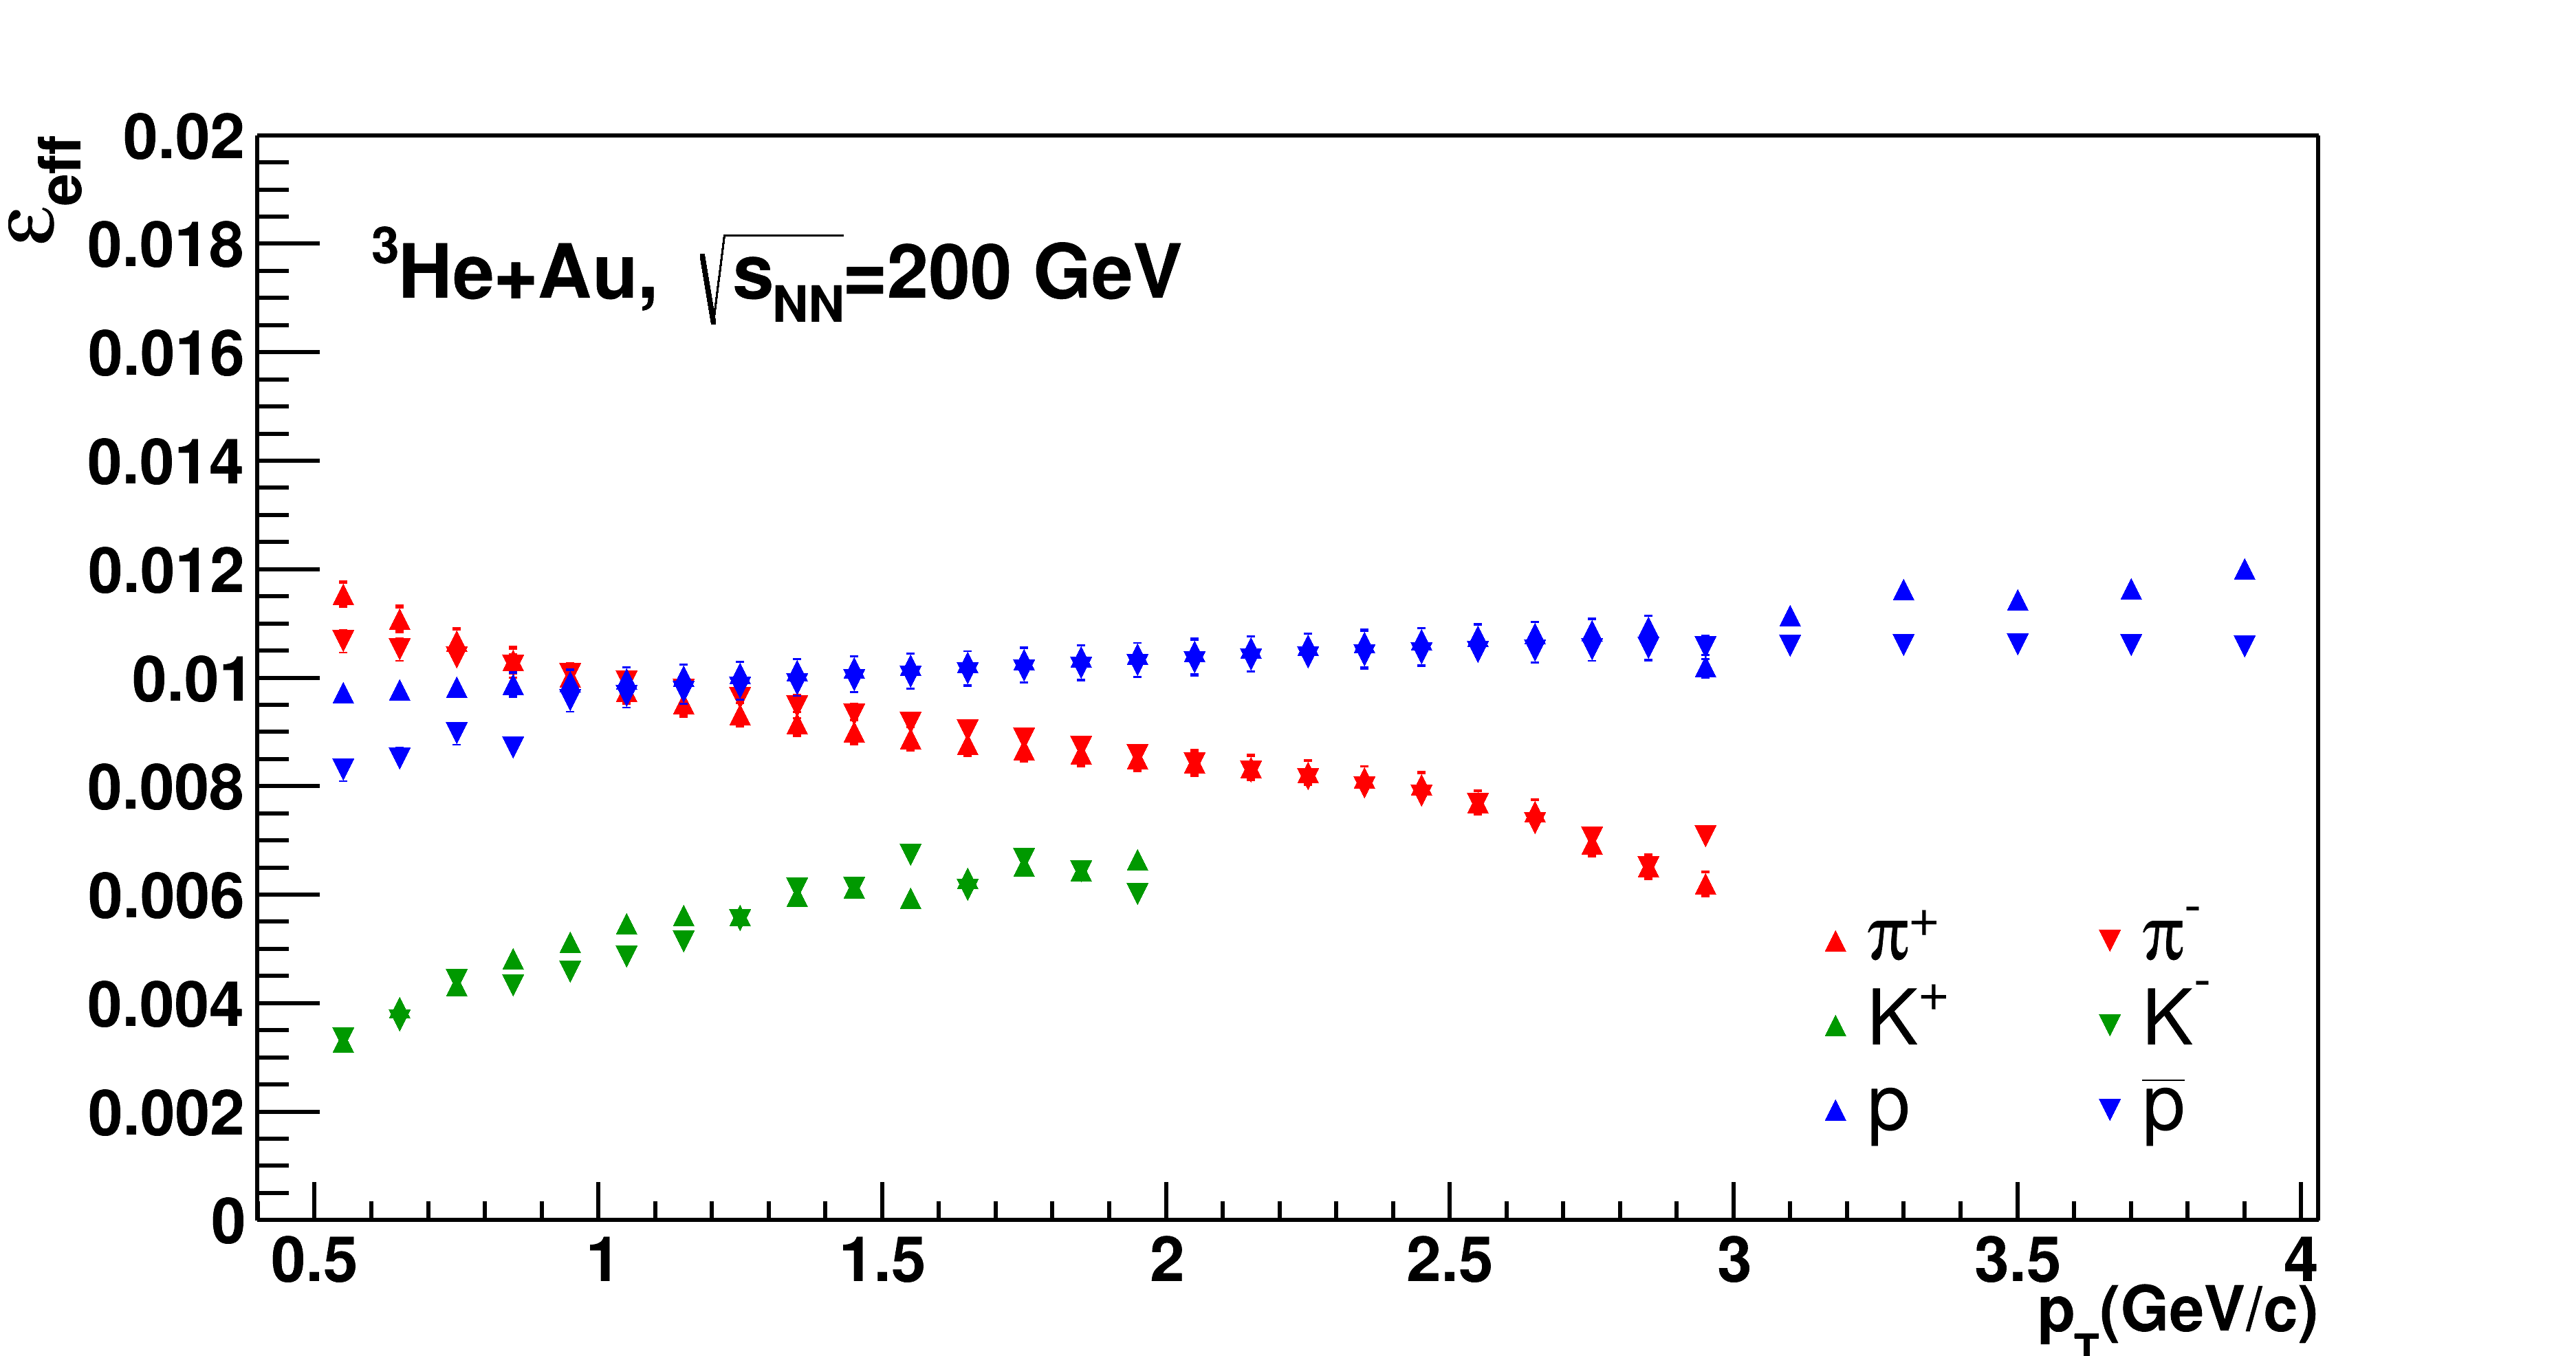
\includegraphics [width=0.9\linewidth]{Methodology/eff_hadron_HeAu.png}
	\caption{Эффективность регистрации заряженных адронов в столкновениях \heau.} 
	\label{img:eff_HeAu}
\end{figure}

\begin{figure}[] 
	\centerfloat
	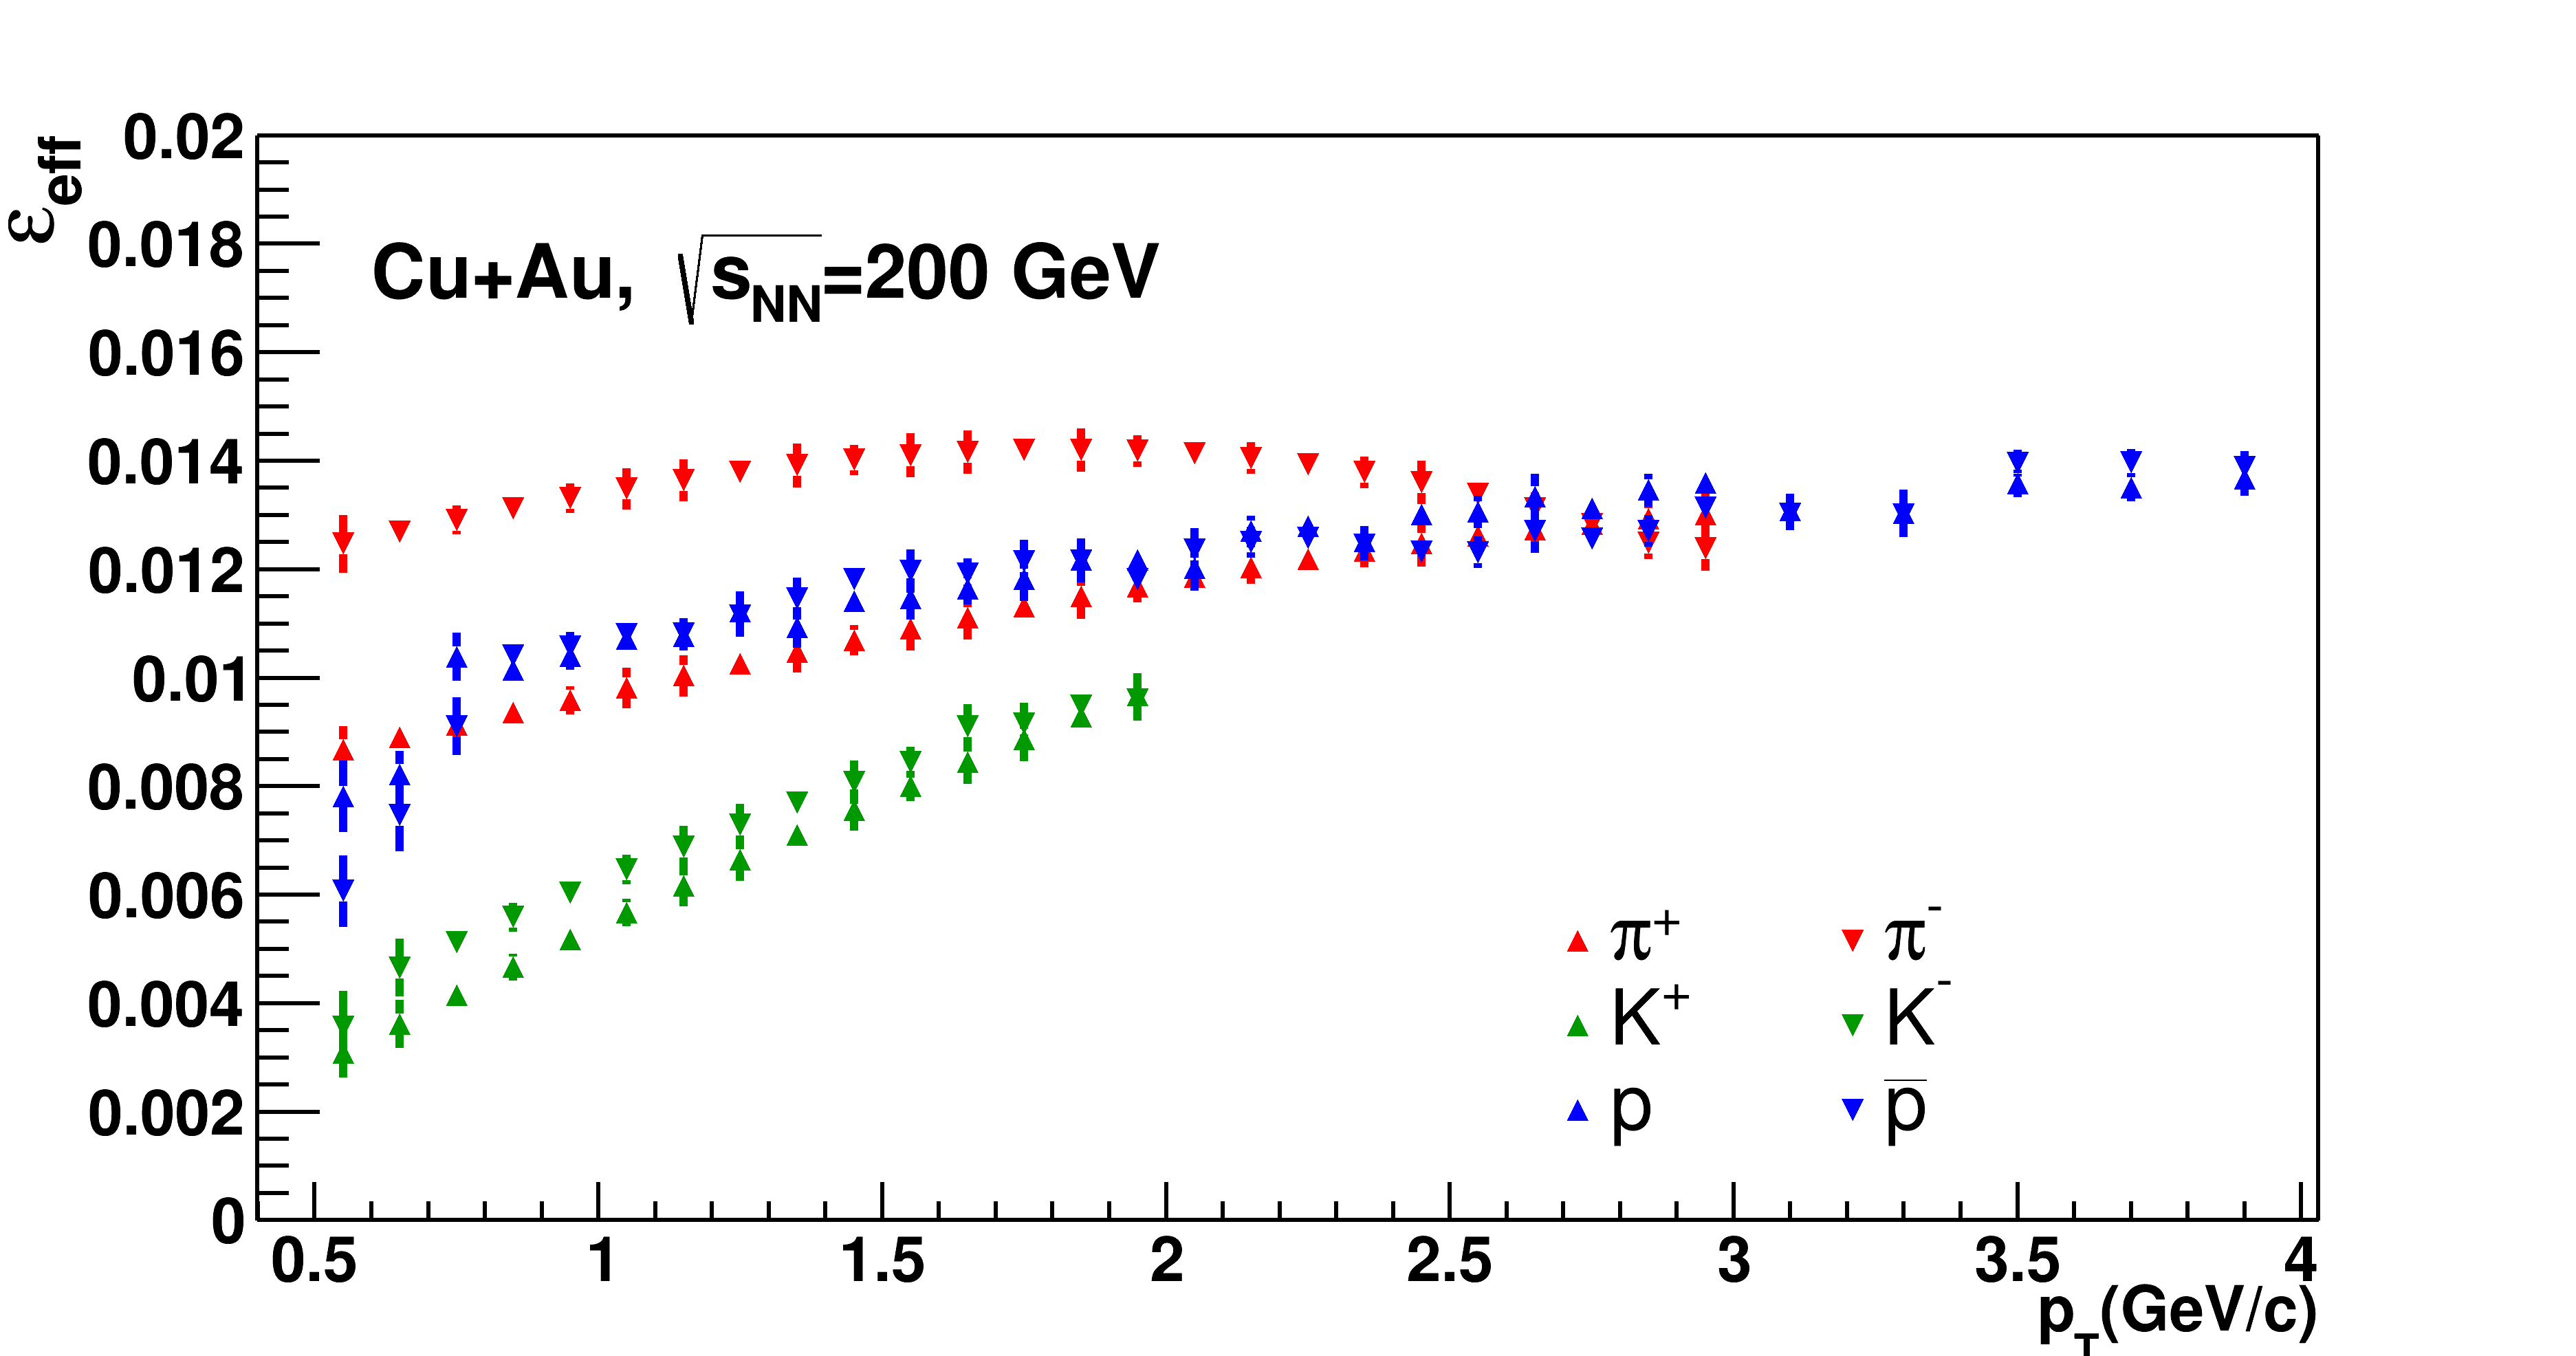
\includegraphics [width=0.9\linewidth]{Methodology/eff_hadron_CuAu.png}
	\caption{Эффективность регистрации заряженных адронов в столкновениях Cu+Au.} 
	\label{img:eff_CuAu}
\end{figure}

\begin{figure}[] 
	\centerfloat
	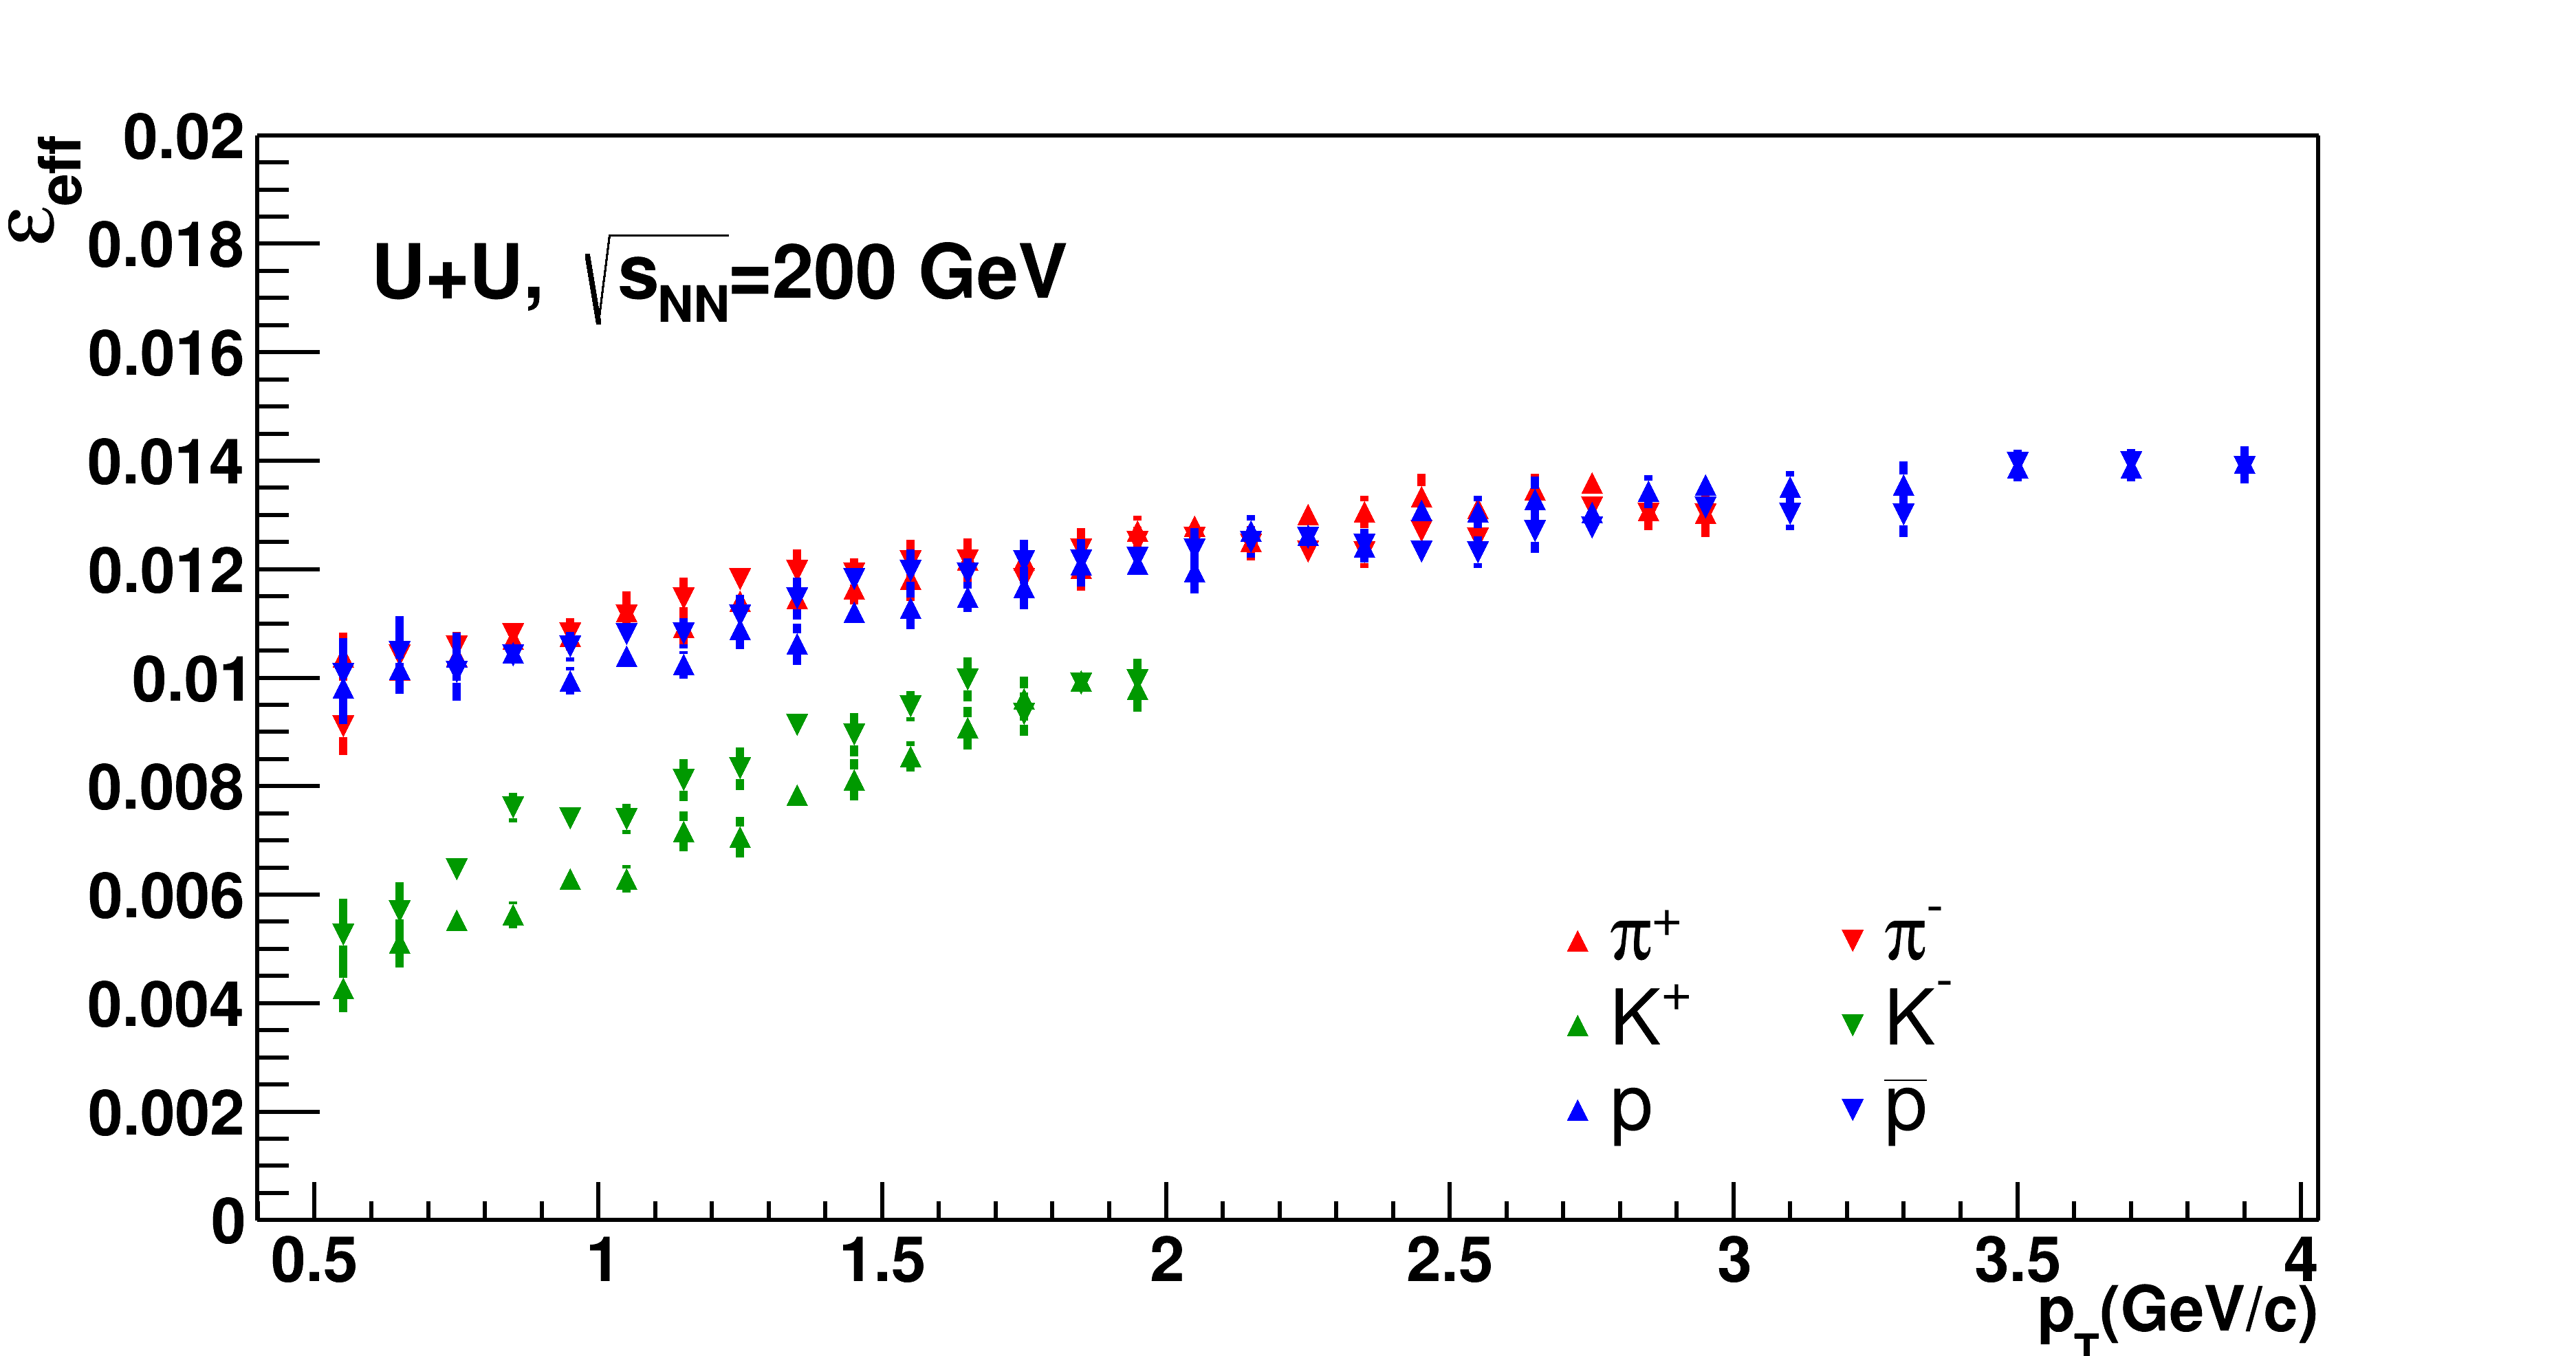
\includegraphics [width=0.9\linewidth]{Methodology/eff_hadron_UU.png}
	\caption{Эффективность регистрации заряженных адронов в столкновениях U+U.} 
	\label{img:eff_UU}
\end{figure}

%====================================================================================

\begin{figure}[] 
	\centerfloat
	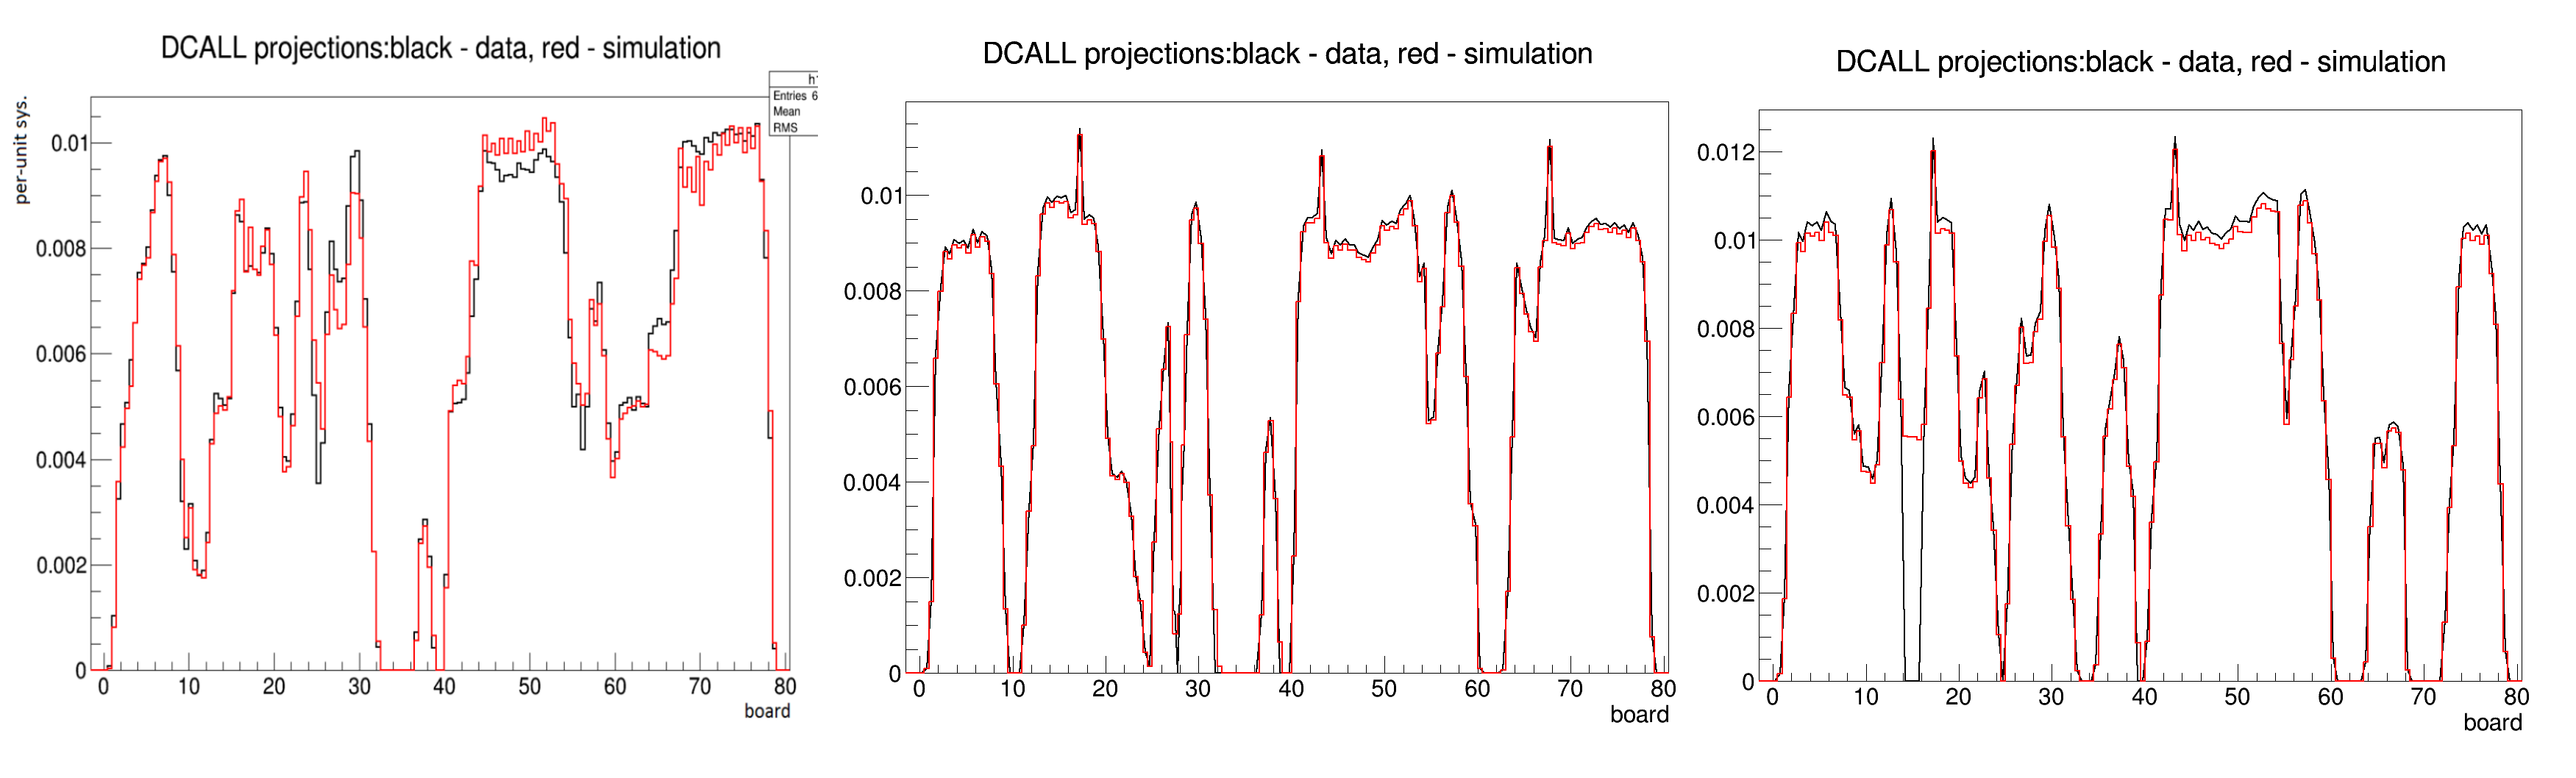
\includegraphics [width=\linewidth]{Methodology/DC_compar.png}
	\caption{DC compar.} 
	\label{img:DC_compar}
\end{figure}

\begin{figure}[] 
	\centerfloat
	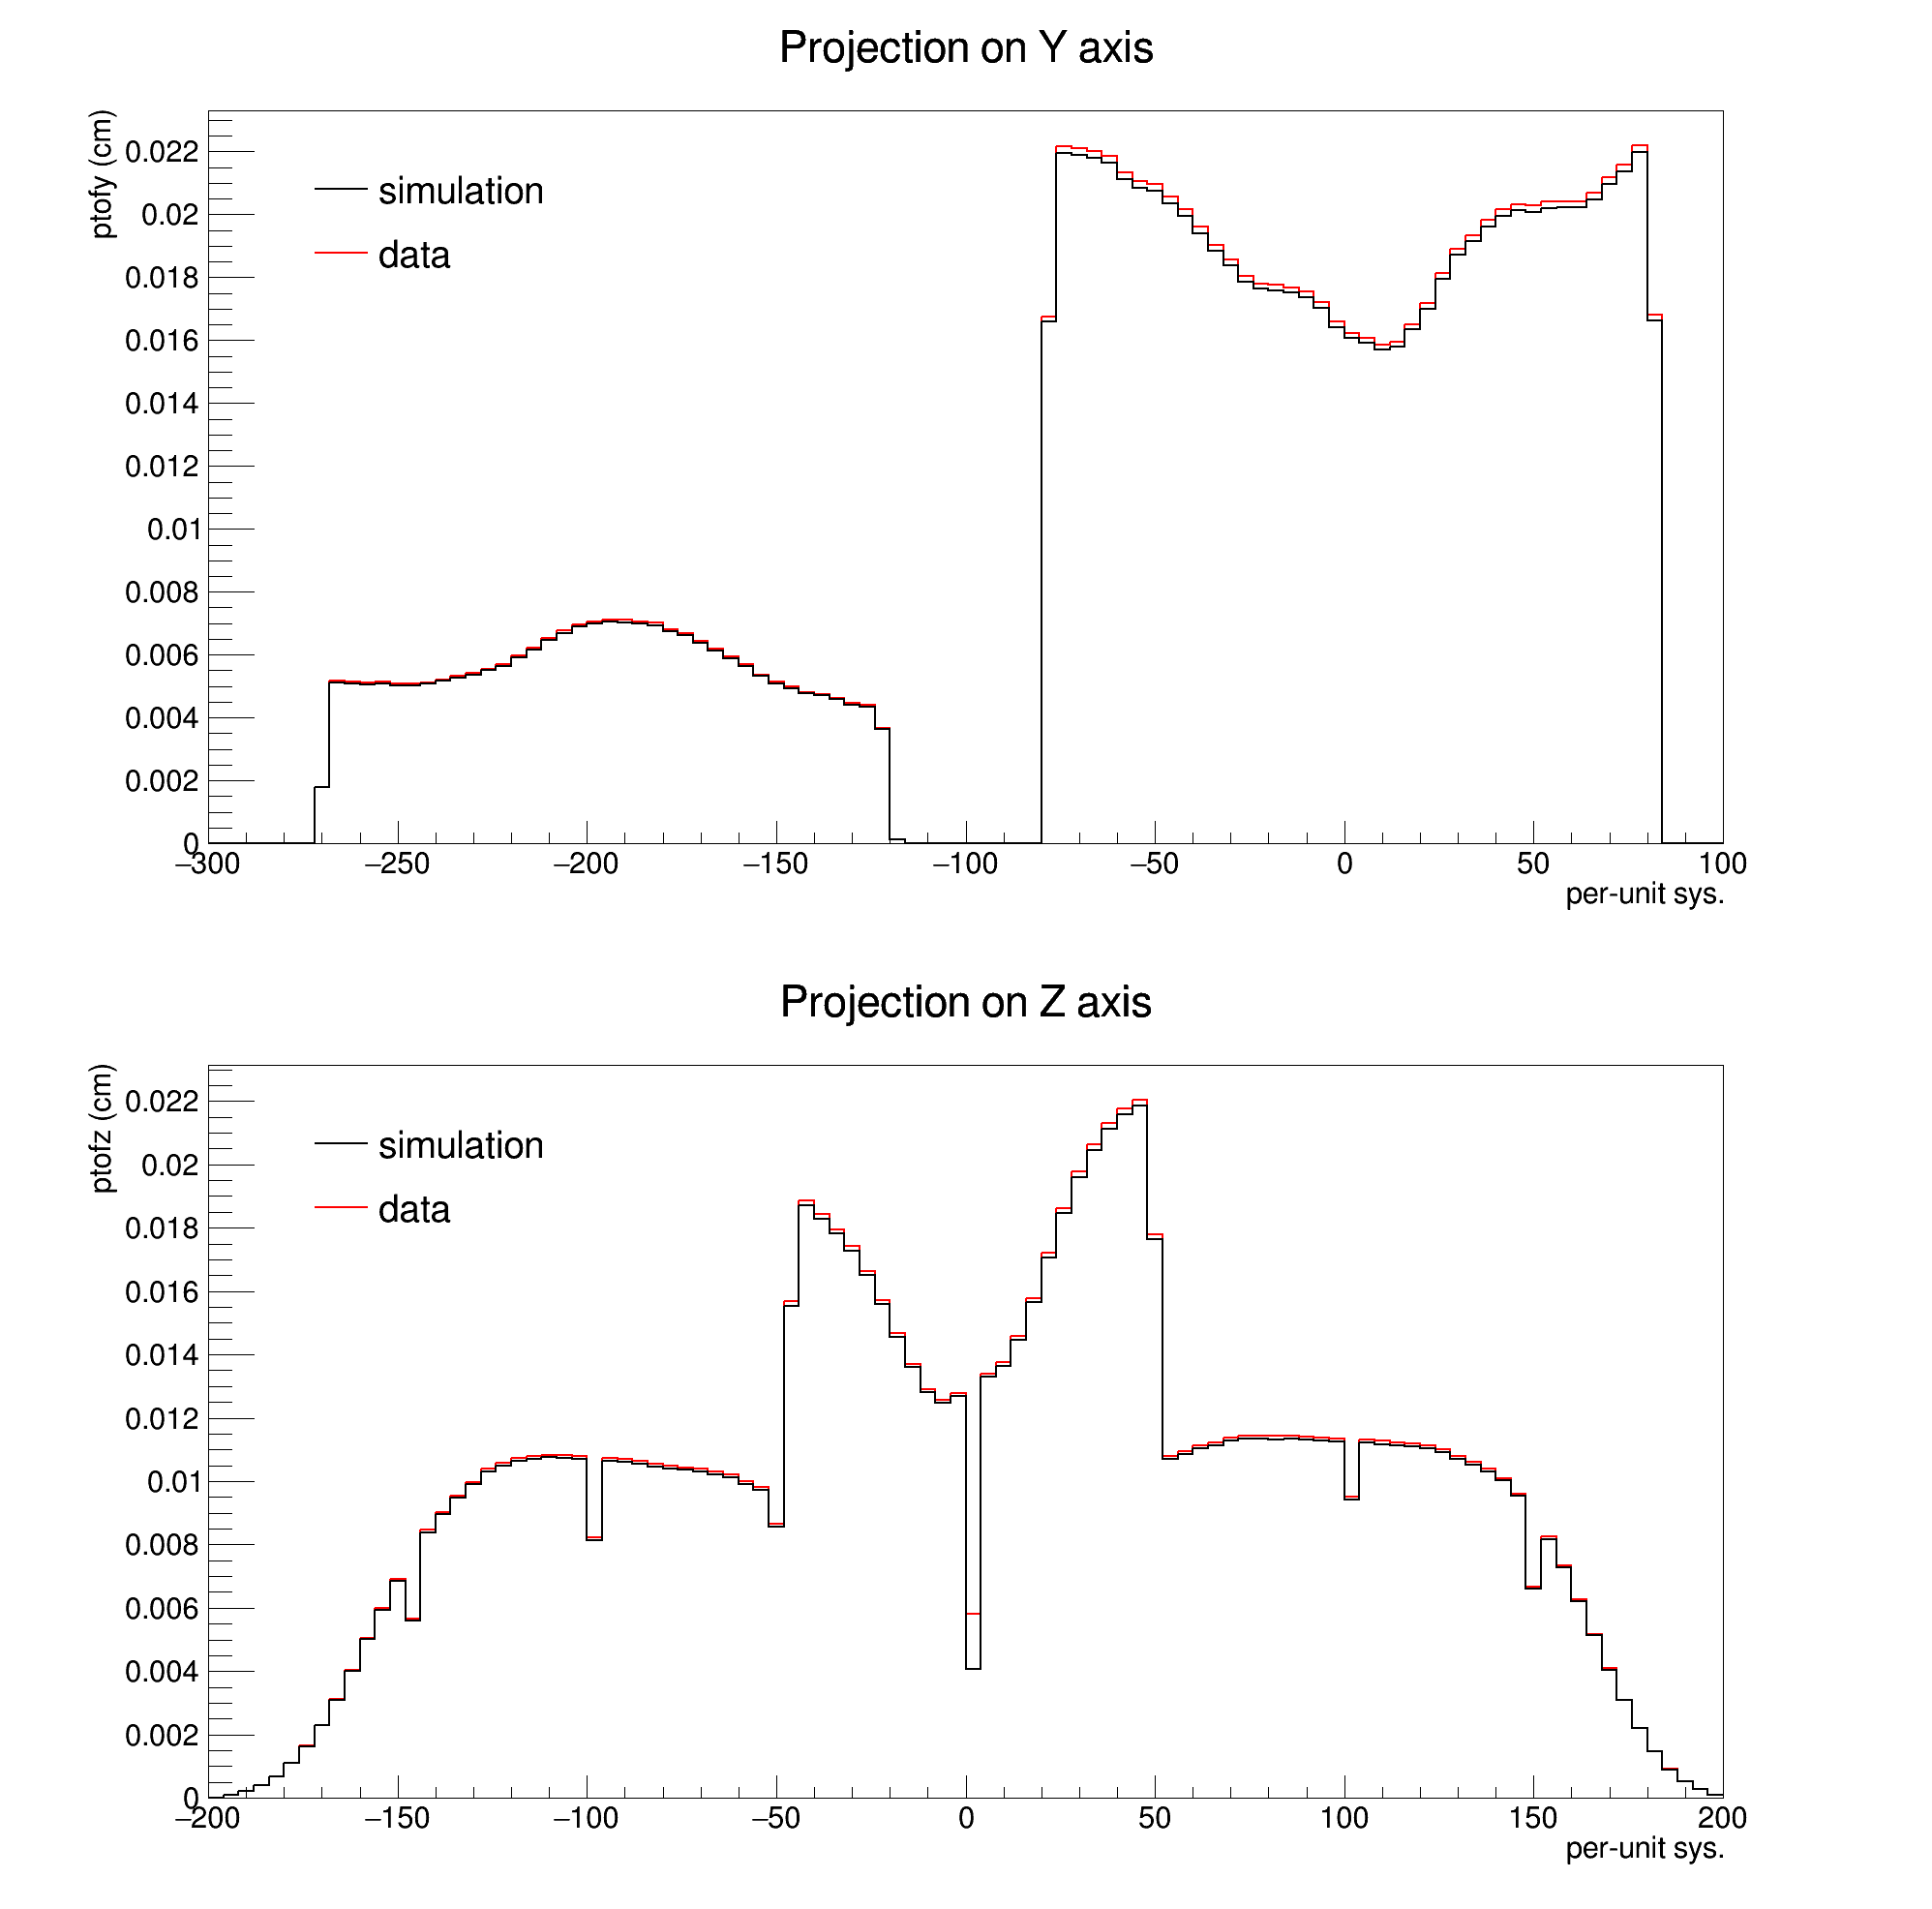
\includegraphics [width=0.9\linewidth]{Methodology/TOF_proj_pAl.png}
	\caption{TOFproj \pal.} 
	\label{img:TOFproj_pAl}
\end{figure}

\begin{figure}[] 
	\centerfloat
	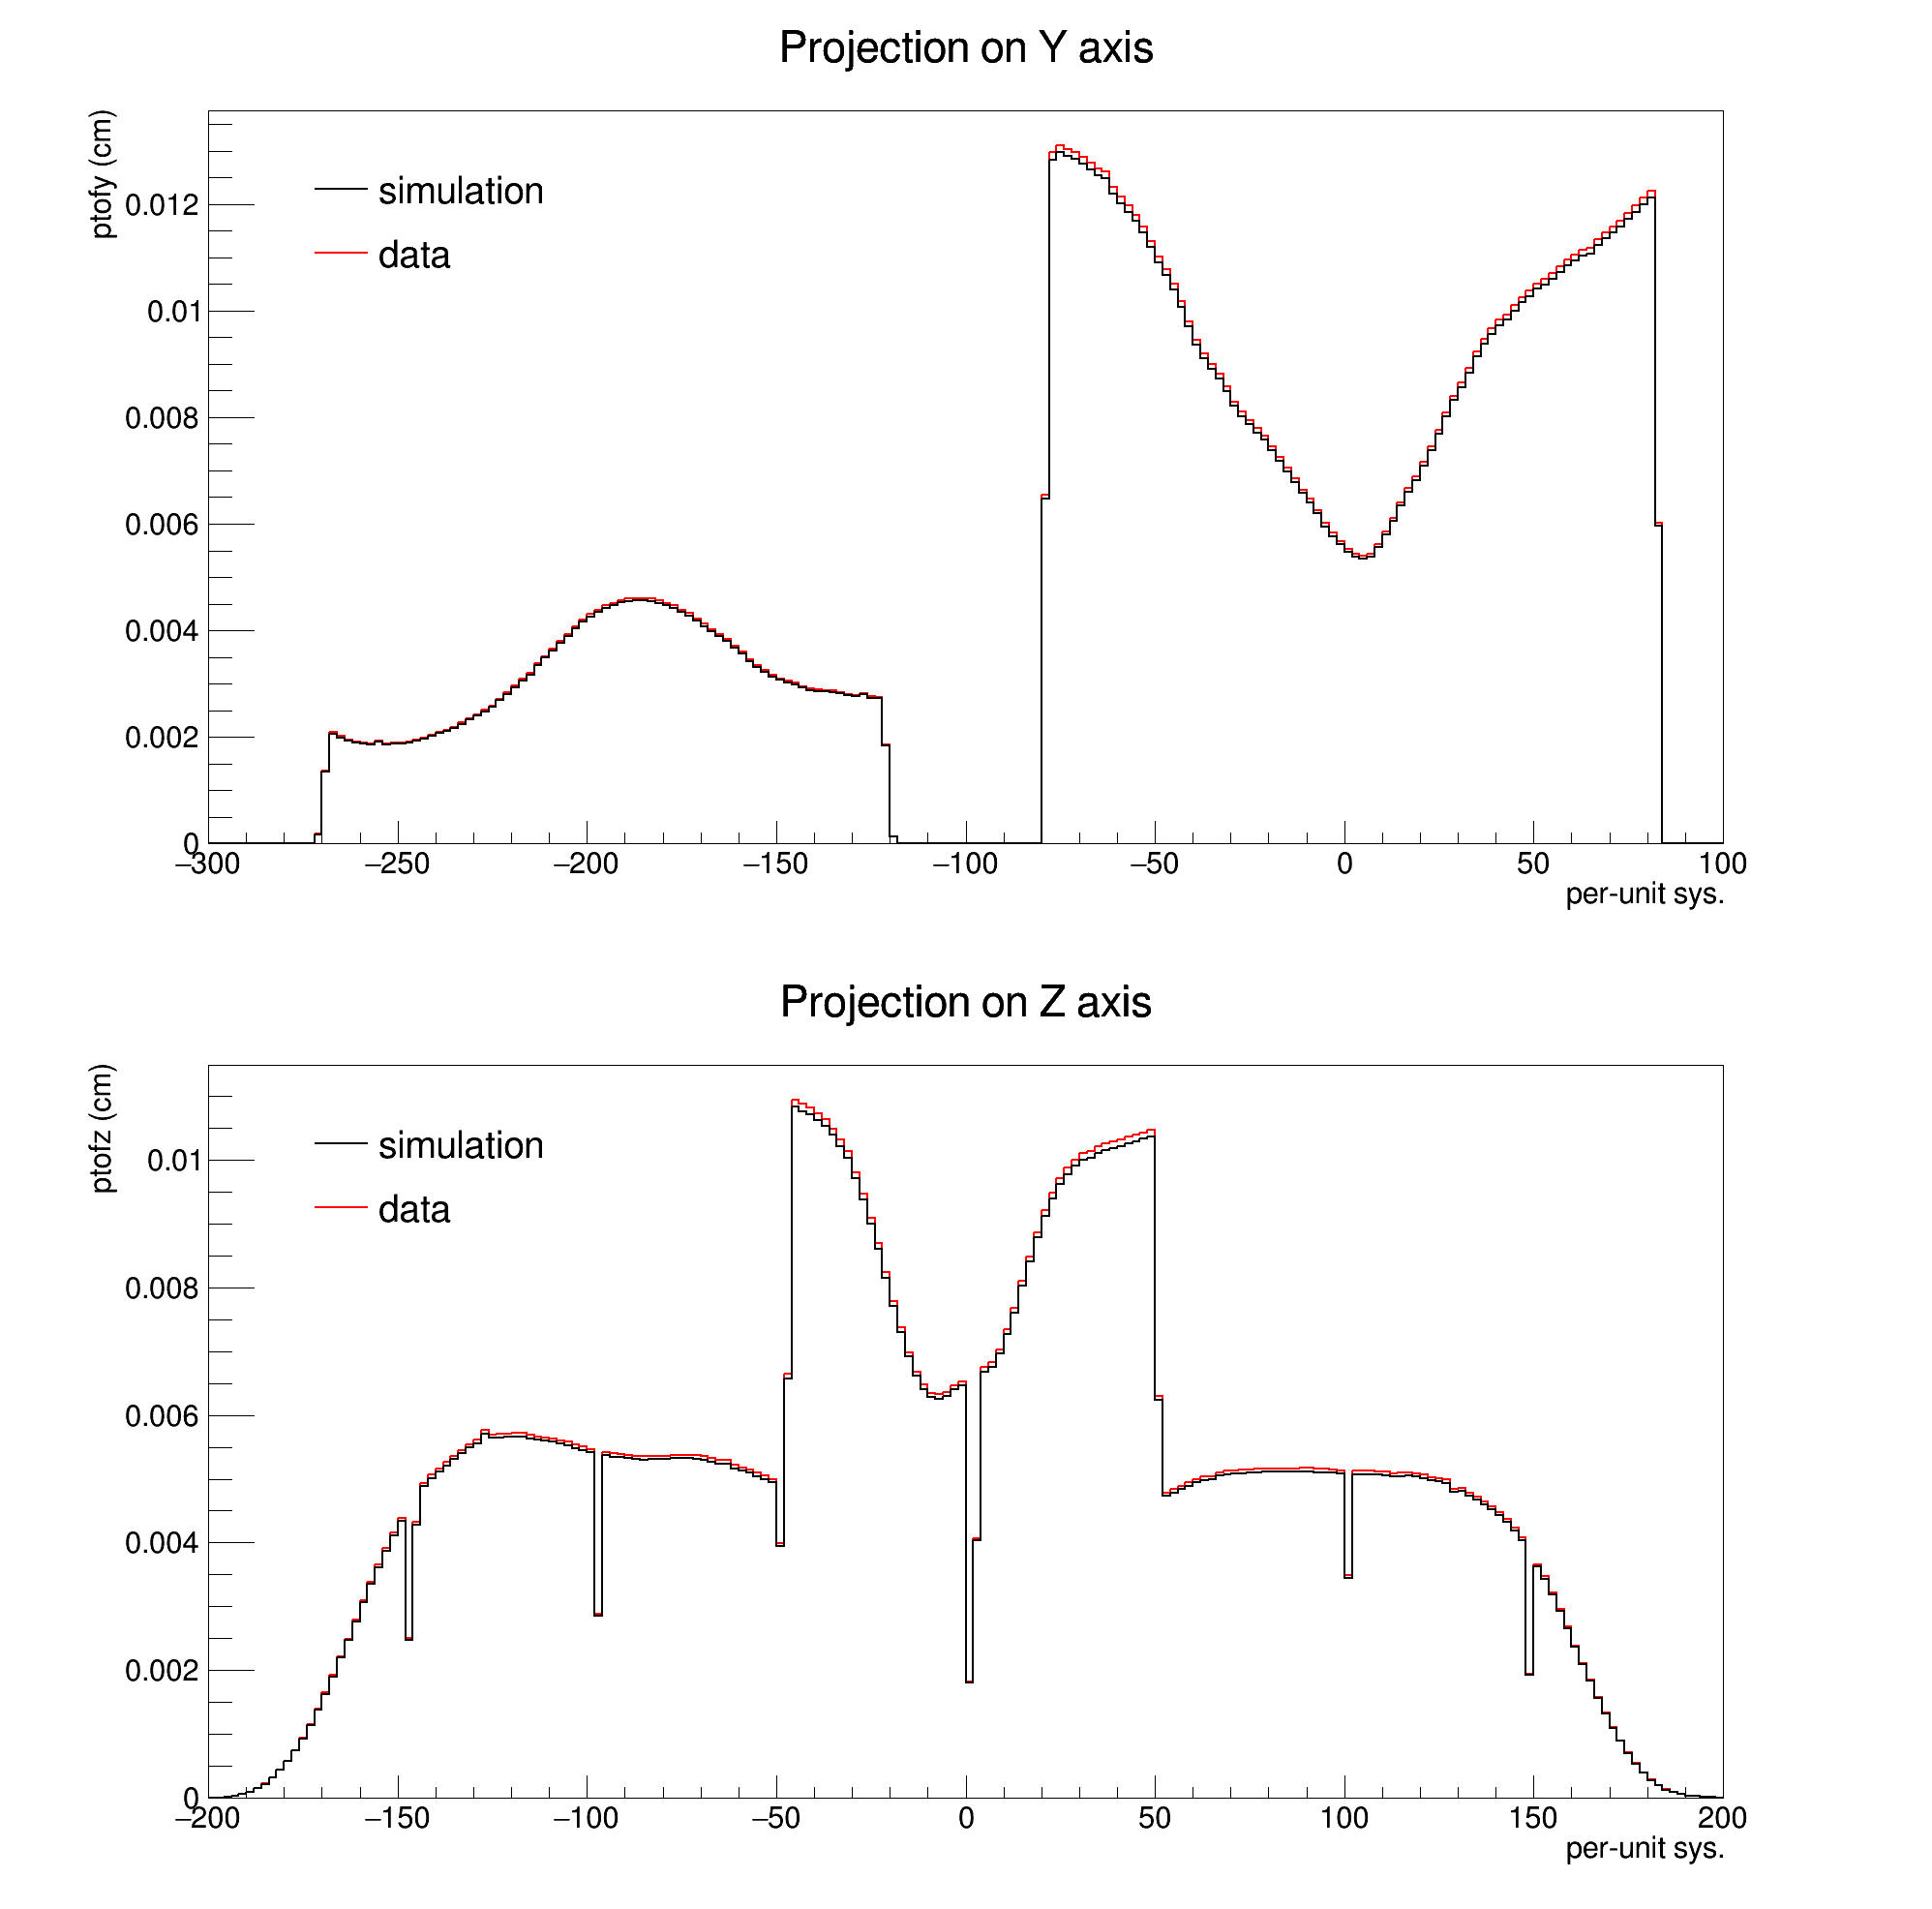
\includegraphics [width=0.9\linewidth]{Methodology/TOF_proj_HeAu.png}
	\caption{TOFproj  \heau.} 
	\label{img:TOFproj_HeAu}
\end{figure}

\begin{figure}[] 
	\centerfloat
	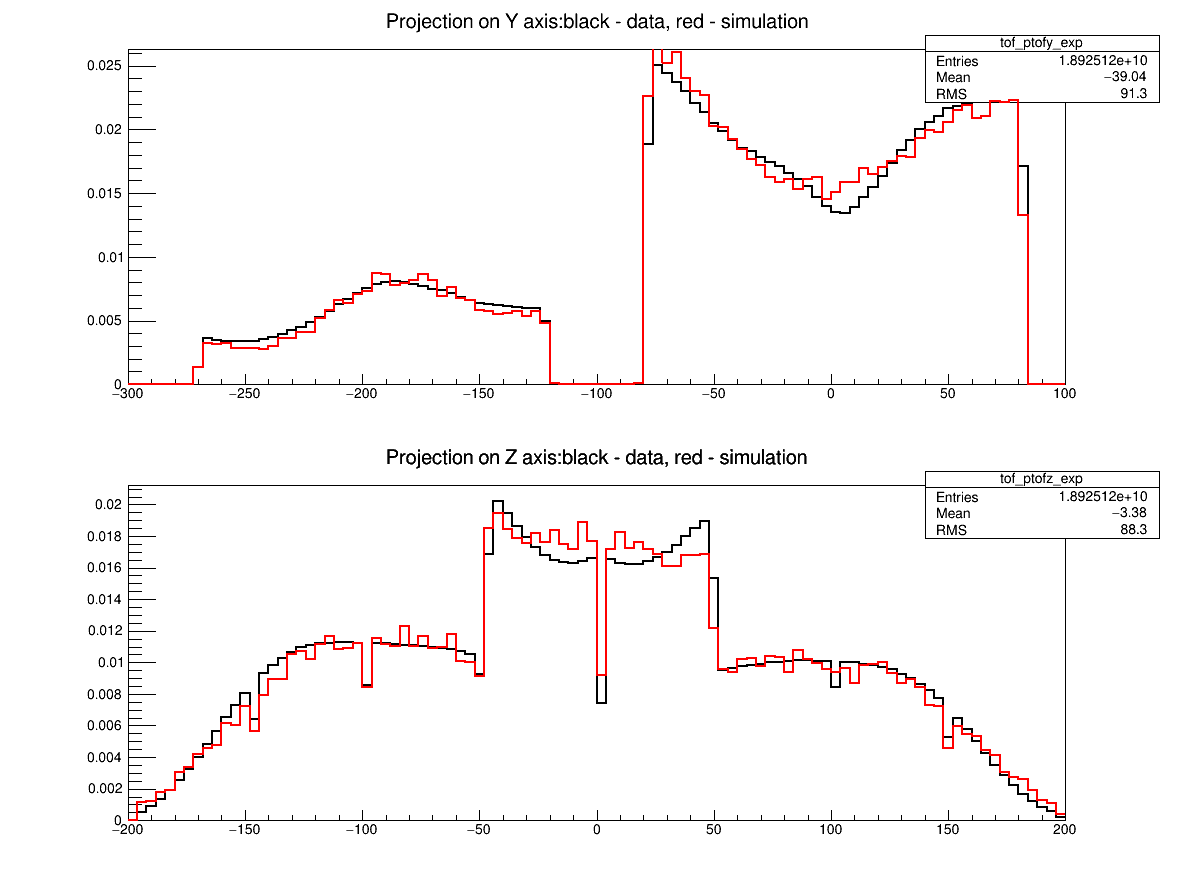
\includegraphics [width=0.9\linewidth]{Methodology/TOF_proj_CuAu.png}
	\caption{TOFproj  Cu+Au.} 
	\label{img:TOFproj_CuAu}
\end{figure}

\begin{figure}[] 
	\centerfloat
	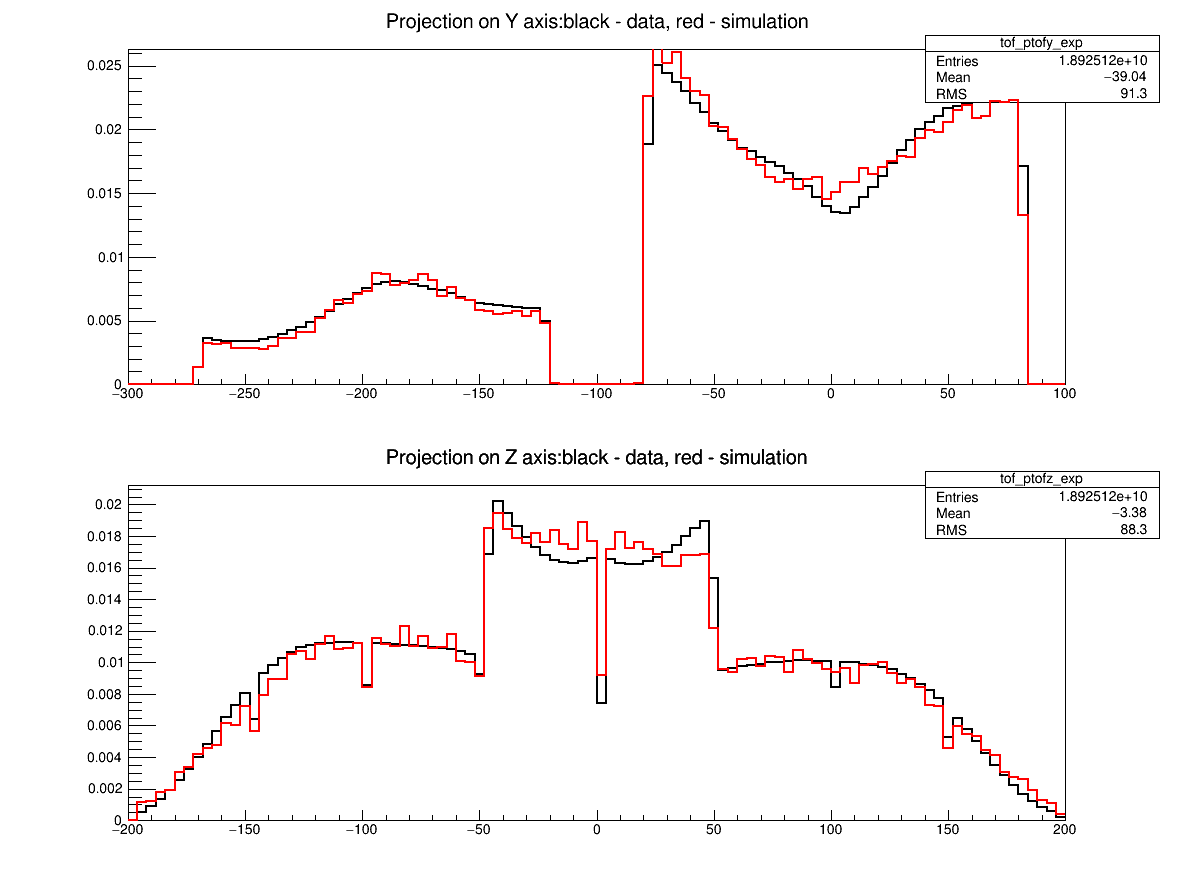
\includegraphics [width=0.9\linewidth]{Methodology/TOF_proj_UU.png}
	\caption{TOFproj U+U.} 
	\label{img:TOFproj_UU}
\end{figure}

\subsection{Коррекция вклада слабых распадов} \label{sect3:FeedDown}
%Weak Decay Correction - поправка слабого взаимодействия
Для оценки количества протонов, родившихся непосредственно столкновении релятивистских ядер, была введена поправка $C_{FD}$, учитывающая образование протонов в результате слабых распадов. Поскольку наибольший вклад в образование протонов вносят $\Lambda$ - барионы, фактор $C_{FD}$ в данной работе был вычислен как процент протонов, образовавшихся в результате распада $\Lambda$ барионов ($N_{\Lambda}^p$), от общей выборки протонов ($N_{tot}^p$ ):
\begin{equation}
	\label{eq:Lambda_pT}
	C_{FD} = \frac{N_{\Lambda}^p}{N_{tot}^p} 
\end{equation}

Для оценки величины $C_{FD}$ было проведено Монте-Карло моделирование рождения $\Lambda$ барионов, с теми же параметрами, которые были использованы для моделирования протонов. Для учета зависимости спектров $\Lambda$ барионов от поперечного импульса, гистограммы были взвешены с весом, вычисляемым по формуле \ref{eq:Lambda_pT}:
\begin{equation}
	\label{eq:Lambda_pT}
	W(p_{T}^{track}) = p_{T} e^{\frac{m_T-m_0}{T}}
\end{equation}
Данная форма выбрана для наиболее точного представления $\Lambda$ и спектра протонов.
Затем в эту долю вносят поправку на коэффициент ветвления и отношения выходов $\Lambda$ барионов к протонам. Были использованы следующие значения отношений $\Lambda/p$:

Измерения $\Lambda$ барионов автоматически учитывают распады $\Sigma^0$ барионов, поскольку $\Sigma^0$ барионы  электромагнитно распадаются на $\Lambda$ и фотоны с коэффициентом ветвления 100 \%. В данной работе не было учтено рождение протонов в других распадах, таких как распады заряженных состояний $\Sigma$-барионов, а также многостранных барионных состояний $\Xi$ и $\Omega$. 

Систематическая неопределенность процента протонов, образовавшихся в результате распада $\Lambda$ барионов, от общей выборки протонов оценивается в 25 \%, что в первую очередь связано с неопределенностью величины отношения $\Lambda/p$. Доля распадных протонов составляет порядка 10–40\%, поэтому изменение отношения $\Lambda /p$ на 25\% приводит к изменению спектра протонов примерно на 2.5–10\%.
На рис. \ref{img:FeedDown} показана зависимость доли распадных протонов и антипротонов от поперечного импульса. 

\begin{figure}[] 
	\centerfloat
	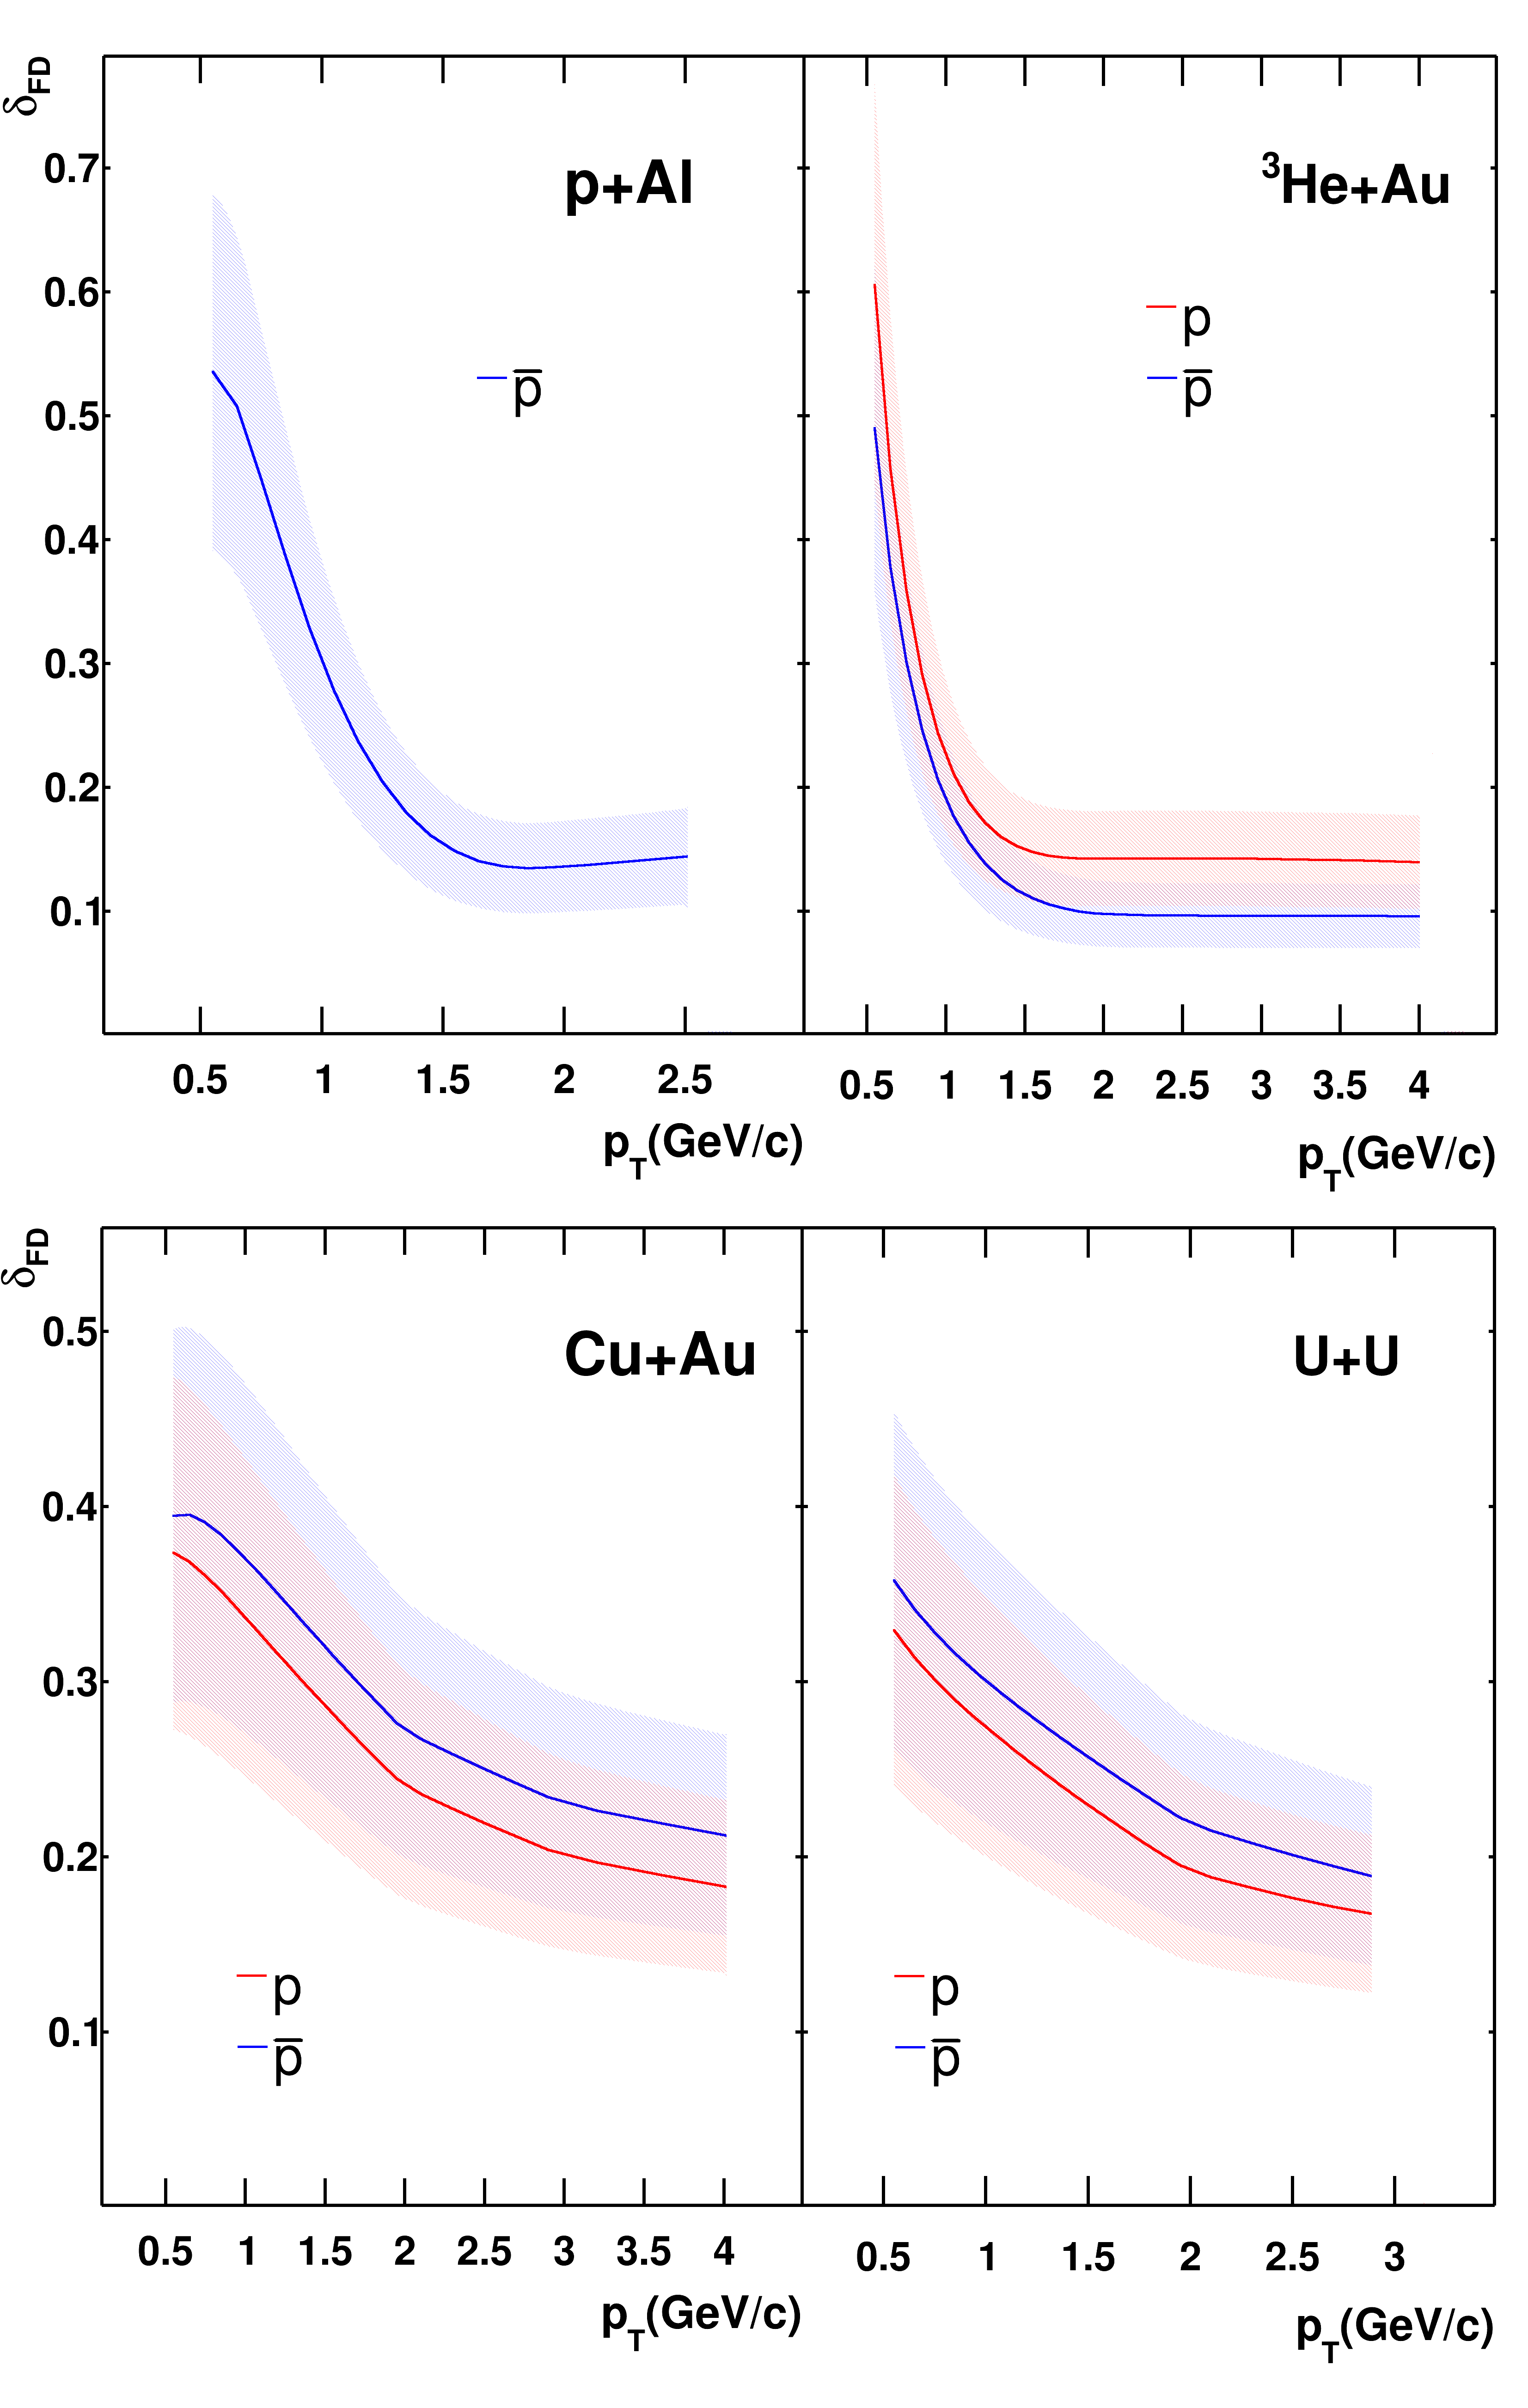
\includegraphics [width=0.7\linewidth]{Methodology/FeedDown.png}
	\caption{Значения $C_{FD}$, вычисленные в столкновениях p+Al, \heau, Cu+Au, U+U  столкновениях. Заштрихованные области обозначают систематические погрешности.} 
	\label{img:FeedDown}
\end{figure}

\section{Систематические неопределенности} \label{sect3:Syst}
Измеряемые величины обладают статистической и систематической неопределенностью. Статистическая неопределенность измерения заряженных адронов обусловлена объемом используемой выборки.
Систематическая неопределенность учитывает возможную ошибку при произвольном выборе параметров анализа (например, выбор параметров аппроксимации пиков, выбор взвешивающей функции), либо ошибку, связанную с неидеальностью воспроизведения условий эксперимента в используемой Монте-Карло модели.
% В данном разделе приведены классификация систематических неопределенностей (п. \ref{sect3:SystClass}), описаны источники систематической неопределенности (п. \ref{sect3:SystSource}) и приведены результаты оценки систематической неопределенности (п. \ref{sect3:SystValues}).

%\subsection{Классификация неопределенностей измерений} \label{sect3:SystClass}
 %Методика определения статистической неопределенности измерения выходов заряженных адронов приведена в п. \ref{sect3:SystValues}. По своей природе, величина статистической неопределенности не коррелирована по поперечному импульсу и центральности.
Систематические неопределенности измерений классифицированы по следующим группам:
\begin{itemize}
	\item неопределенность <<типа A>> полностью не коррелирована по поперечному импульсу и центральности. 
	\item неопределенность <<типа B>> коррелирована по поперечному импульсу, однако точный закон корреляции не известен. К неопределенностям типа B относят все систематические неопределенности, которые не являются неопределенностями типов A и C. Для всех результатов измерений неопределенность типа A квадратично суммируется со статистической неопределенностью.
	\item неопределенность <<типа C>> полностью коррелированы по поперечному импульсу, т.е. сдвигают измеренные мезонные выходы в область больших либо меньших значений одинаково во всем диапазоне поперечного импульса. В данной работе неопределенность типа C обусловлена неопеределенностью измерения значений \Ncoll.
\end{itemize}

\subsection{Источники систематических неопределенностей измерения заряженных адронов} \label{sect3:SystSource}
Cистематическая неопределенность определения спектров рождения заряженных адронов может исходить от неточности определнения следующих величин: первичного выхода заряженных адронов, эффективности регистрации заряженных адронов, а также отношения величин первичного выхода и эффективности регистрации. Ниже представлено описание источников систематической неопределенности измерений, учитываемые в настоящей работе. 

\bfseries Неопределенности, связанные с исключением мертвых областей дрейфовой камеры.
\mdseries
Данная систематическая неопределенность связана с произвольностью определения границ мертвых областей исключаемых из дальнейшего рассмотрения. Для оценки величины такой неопределенности, было проведено сравнение значений первичных выходов заряженных адронов, измеренных стандартным способом, а также двумя альтернативными способами: без  исключения мертвых областей дрейфовой камеры, а также с исключением мертвых областей, уменьшенных на 5 мрад по сравнению со стандартным методом. 


\bfseries Неопределеннсть, связанная с ограничением z-координаты вершины столкновения при отборе событий. 
\mdseries
Для оценки неопределеннсти, связанной с ограничением z-координаты вершины столкновения при отборе событий проводится сравнение результатов измерения заряженных адронов со стандартным критерием отбора данных по zed $|zed|<70$ и измерения заряженных адронов, с условием на zed $|zed|<40$ 

\bfseries Неопределенность идентификации частиц во времяпролетной камере.
\mdseries
вызвана погрешностью определения параметров функции \ref{eq:TOFgaus_approx} и значений  $\sigma_h$ и $m_h$ (п. \ref{sect3_PID}). Данная неопределенность была оценена путем сравнения первичных выходов заряженных адронов, идентифицированных согласно стандартным критериям, описанным в п. \ref{sect3_PID}, а также идентифицированных с использованием условий $ m^2_h -2.5\sigma_h < m^2 < m^2_h +2.5\sigma_h $ и  $ m^2_h -1.5\sigma_h < m^2 < m^2_h +1.5\sigma_h $.

\bfseries Неопределенность, связанная с ограниченным аксептансом дрейфовой камеры
\mdseries
Систематическая неопределенность, связанная с неидеальностью воспроизведения геометрии электромагнитного калориметра в Монте-Карло модели, оценивалась по изменению отношения данных к моделирования (см.  рис. \ref{img:DC_compar}). Это изменение было получено путем выбора различных областей для нормировки результатов моделирования на представление того же общего интеграла, что и в экспериментальных данных. Было выбрано 10 различных областей вдоль оси номеров плат ДК. Каждая область поочередно использовалась для нормировки распределений треков в ДК, полученных из экспериментальных данных и моделирования. Для каждой из 10 проведенных нормировок были вычислены отношения полных интегралов распределений треков в ДК, полученных из экспериментальных данных и моделирования. Итоговое значение рассматриваемой погрешности было вычислено как среднеквадратичное значение отношения 10 полученных данных к интегралам моделирования. 

\subsection{Значения систематических неопределенностей спектров заряженных адронов} \label{sect3:SystValues}
Значения систематических неопределенностей измерения выхода заряженных адрнов в зависимости от их поперечного импульса со стороны различных источников неопределенности приведены в таблицах \ref{table:systDC}-\ref{table:systPID} приложения \label{AppendixA}. Основным источником систематической неопределенности измерения выхода заряженных адронов являются неопределенности, связанные с исключением мертвых областей дрейфовой камеры и идентификации частиц во времяпролетной камере. Соответствующая относительная величина систематической неопределенности увеличивается от 2 до 9\% с ростом поперечного импульса. 
Итоговые значения систематических погрешностей вычислялись как среднеквадратичное значение погрешностей различных типов. Полученные итоговые значения систематических неопределенностей приведены в таблице \ref{table:systTotal}.

\begin{table}[]
	\caption{Значения систематических погрешностей змерений заряженных адронов}
	\label{table:systTotal}
	
	\begin{tabularx}{\linewidth}
		{ 
			| >{\raggedright\arraybackslash}X 
			| >{\centering\arraybackslash}X 
			| >{\centering\arraybackslash}X 
			| >{\centering\arraybackslash}X 
			| >{\centering\arraybackslash}X 
			| >{\centering\arraybackslash}X 
			| >{\centering\arraybackslash}X | }
		\hline
		&\pt (ГэВ/c)     &  0.5 - 1 & 1 - 1.5 & 1.5 - 2 & 2.5 - 3 & 2.5 - 3     \\ \hline
		\multirow{6}{*}{p+Al}  
		&  \pip  &      9.7  &      10.5  &      11.3  &     -  &      -    \\ \cline{2-7}
		&  \pim  &      8.7  &      11  &      10.5  &      -  &      -    \\ \cline{2-7}
		&  \Kp  &      7.9  &      10.2  &      13.7  &      -  &      -    \\ \cline{2-7}
		&  \Km  &      7.7  &      9.9  &      15  &      -  &      -    \\ \cline{2-7}
		&  \prot  &      10.3  &      11.5  &      12.4  &      13.1  &      16.5    \\ \cline{2-7}
		&  \aprot  &      8.4  &      8.6  &      10.3  &      10.9  &      12.8    \\ \hline
		\multirow{6}{*}{\heau}
		&  \pip  &      5.7  &      4.2  &      5.7  &      6.7  &      -    \\ \cline{2-7}
		&  \pim  &      11.6  &      11.3  &      10.5  &      9.1  &      -    \\ \cline{2-7}
		&  \Kp  &      8.3  &      8.6  &      10  &      -  &      -    \\ \cline{2-7}
		&  \Km  &      8.7  &      9.9  &      11.3  &      -  &      -    \\ \cline{2-7}
		&  \prot  &      8.6  &      8.6  &      8.8  &      8.5  &      8.8    \\ \cline{2-7}
		&  \aprot  &      9.1  &      10  &      10.4  &      10.3  &      10.6    \\  \hline
		\multirow{6}{*}{Cu+Au}
		&  \pip  &      10.2  &      10.9  &      10.5  &      9.9  &      -    \\ \cline{2-7}
		&  \pim  &      8.9  &      10.1  &      10  &      10.5  &      -    \\ \cline{2-7}
		&  \Kp  &      10.2  &      8.3  &      7.5  &      -  &      -    \\ \cline{2-7}
		&  \Km  &      10  &      7.7  &      8.6  &      -  &      -    \\ \cline{2-7}
		&  \prot  &      9  &      9  &      9.7  &      11.3  &      -   \\ \cline{2-7}
		&  \aprot  &      9.3  &      7.9  &      7.7  &      8.8  &      -    \\  \hline
		\multirow{6}{*}{U+U}
		&  \pip  &      16.8  &      16.5  &      14.7  &      13.7  &      -    \\ \cline{2-7}
		&  \pim  &      6.2  &      8.8  &      9.4  &      16.9  &      -    \\ \cline{2-7}
		&  \Kp  &      10.2  &      8.3  &      8.3  &      -  &      -    \\ \cline{2-7}
		&  \Km  &      8.8  &      7.6  &      8.5  &      -  &      -    \\ \cline{2-7}
		&  \prot  &      10  &      9.8  &      9.8  &      11.2  &      -    \\ \cline{2-7}
		&  \aprot  &      10.3  &      10  &      9.1  &      10.5  &     -   \\  \hline
		
	\end{tabularx}
\end{table}

\section{Инвариантные спектры по поперечному импульсу} \label{sectRes_spectra}
Для понимания адронно-адронных столкновений высоких энергий Ферми предложил следующий статистический метод [7]. Из-за насыщения фазового пространства рождение множества частиц в результате элементарных столкновений высоких энергий согласуется с тепловым описанием [7, 8, 9]. В столкновениях тяжелых ионов можно ожидать гидродинамического поведения, то есть локального теплового равновесия и коллективного движения, из-за большого числа вторичных рассеяний. Адроны в конечном состоянии являются наиболее многочисленным и доминирующим источником информации о ранней стадии столкновений. Спектры адронов по поперечному импульсу и быстроте зависят от температуры и параметров коллективного потока частиц. Отношения спектров частиц чувствительны к химическим свойствам системы и механизму образования частиц.
% Недавний обзор существующих данных, полученных в основном из CERN-SPS, можно найти в литературе [10].

Измерение инвариантных спектров по поперечному импульсу является одним из основных инструментов для изучения рождения частиц в столкновениях релятивистских ионов.
Инвариантные спектры по поперечному импульсу вычисляются согласно формуле \ref{eq:pTspectra}:
\begin{equation}
	\label{eq:pTspectra}
	\frac{1}{2\pi p_T} \frac{d^2 N}{dp_T dy}=\frac{1}{2\pi p_T}\frac{N_h}{N_{evt} \varepsilon_{eff} \Delta p_T \Delta y}
\end{equation}
где $\Delta p_T$ – диапазон поперечных импульсов, $\Delta y$ – диапазон быстрот, $N_h$ - количество заряженных адронов $h$, зарегистрированных в диапазонах  $\Delta p_T, \Delta y$,  $\varepsilon_{eff}$ - эффективность регистрации адронов $h$.
Инвариантные спектры по поперечному импульсу связаны с распределением по инвариантной массе следующим образом:
\begin{equation}
	\label{eq:mTspectra}
	\begin{split}
		\frac{1}{2\pi p_T} \frac{d^2 N}{dp_T dy}=
		\frac{1}{2\pi \sqrt{m_T^2-m_0^2}} \frac{d^2 N}{d(\sqrt{m_T^2-m_0^2})dy}=\\
		\frac{1}{2\pi \sqrt{m_T^2-m_0^2}} \frac{d^2 N \sqrt{m_T^2-m_0^2}}{m_T dm_Tdy}=\frac{1}{2\pi m_T} \frac{d^2 N}{dm_Tdy}
	\end{split}
\end{equation}
где $m_0$ - масса адрона, $m_T = \sqrt{p_{T}^{2}+m_0^2}$.


Согласно моделям термодинамики \cite{Thermal1, Thermal2} в области $m_T<$1.5 ГэВ/с спектры имеют экспоненциальную форму и могут быть описаны  зависимостью \ref{eq:mTspectraEXP}:
\begin{equation}
	\label{eq:mTspectraEXP}
	\frac{1}{2\pi m_T} \frac{d^2 N}{dm_T dy}=\frac{1}{2\pi T (T+m_0)}\cdot A \cdot exp{\frac{-m_T -m_0}{T}}
\end{equation}
$T$ - параметр обратного наклона спектра, $A$ - нормировочный коэффициент, содержащий информацию о множественности рождения частиц в данном диапазоне быстрот $dN/dy$.
%В области \mt$>2$ ГэВ/с спектры начинают проявлять степенную зависимость от \mt. 

Параметр обратного наклона $T$ пропорционален средней поперечной кинетической энергии, следовательно, в рамках термодинамических моделей, проявляет следующую зависимость от массы адрона (см. раздел \ref{ch1/hydro}):
$$ T \sim T_{thermal}+m_0 \cdot \langle u_T ^2 \rangle$$


\section{Факторы ядерной модификации}
Для количественного сравнения выходов адронов в ядро-ядерных и протон-протонных соударениях были вычислены факторы ядерной модификации (\rab). Для столкновений ядер A и B значение \rab \ определяется соотношением
\begin{equation}
	\label{eq:rab}
	R_{AB}=\frac{1}{N_{coll}}\frac{d^2 N_{A+B}/dp_T dy}{d^2 N_{p+p}/dp_T dy} 
\end{equation}
где \Ncoll \ – количество парных нуклон-нуклонных соударений, 
$d^2 N_{A+B}/dp_T dy$ и $d^2 N_{p+p}/dp_T dy$ – инвариантные спектры адронов в столкновениях A+B и $p+p$ соответственно.



           % Глава 3
\chapter{Результаты} \label{chapt_Res}

\section{Инвариантные спектры по поперечному импульсу} \label{sectRes_spectra}

Инвариантные спектры по поперечному импульсу были вычислены согласно формуле \ref{eq:spectra}.
\begin{equation}
	\label{eq:spectra}
	\frac{1}{2\pi p_T} \frac{d^2 N}{dp_T dy}=\frac{1}{2\pi p_T}\frac{N_h}{N_{evt} \varepsilon_{eff} \Delta p_T \Delta y}
\end{equation}
где $\Delta p_T$ – диапазон поперечных импульсов;

$\Delta y$ – диапазон быстрот;

$N_h$ - количество заряженных адронов $h$, зарегистрированных в диапазонах  $\Delta p_T, \Delta y$;

\eff~ -- эффективность регистрации адронов $h$. 

Для оценки значения величины \eff~ было проведено Монте-Карло моделирование (см. Раздел \ref{sect3:EffRec}).
Инвариантные спектры по поперечному импульсу, измеренные для положительно и отрицательно заряженных адронов в различных центральностях $p$+Al, \heau, Cu+Au и U+U столкновений представлены на Рисунке \ref{img:SpectraPt}. 

\begin{comment}
\begin{figure}[] 
	\centerfloat
	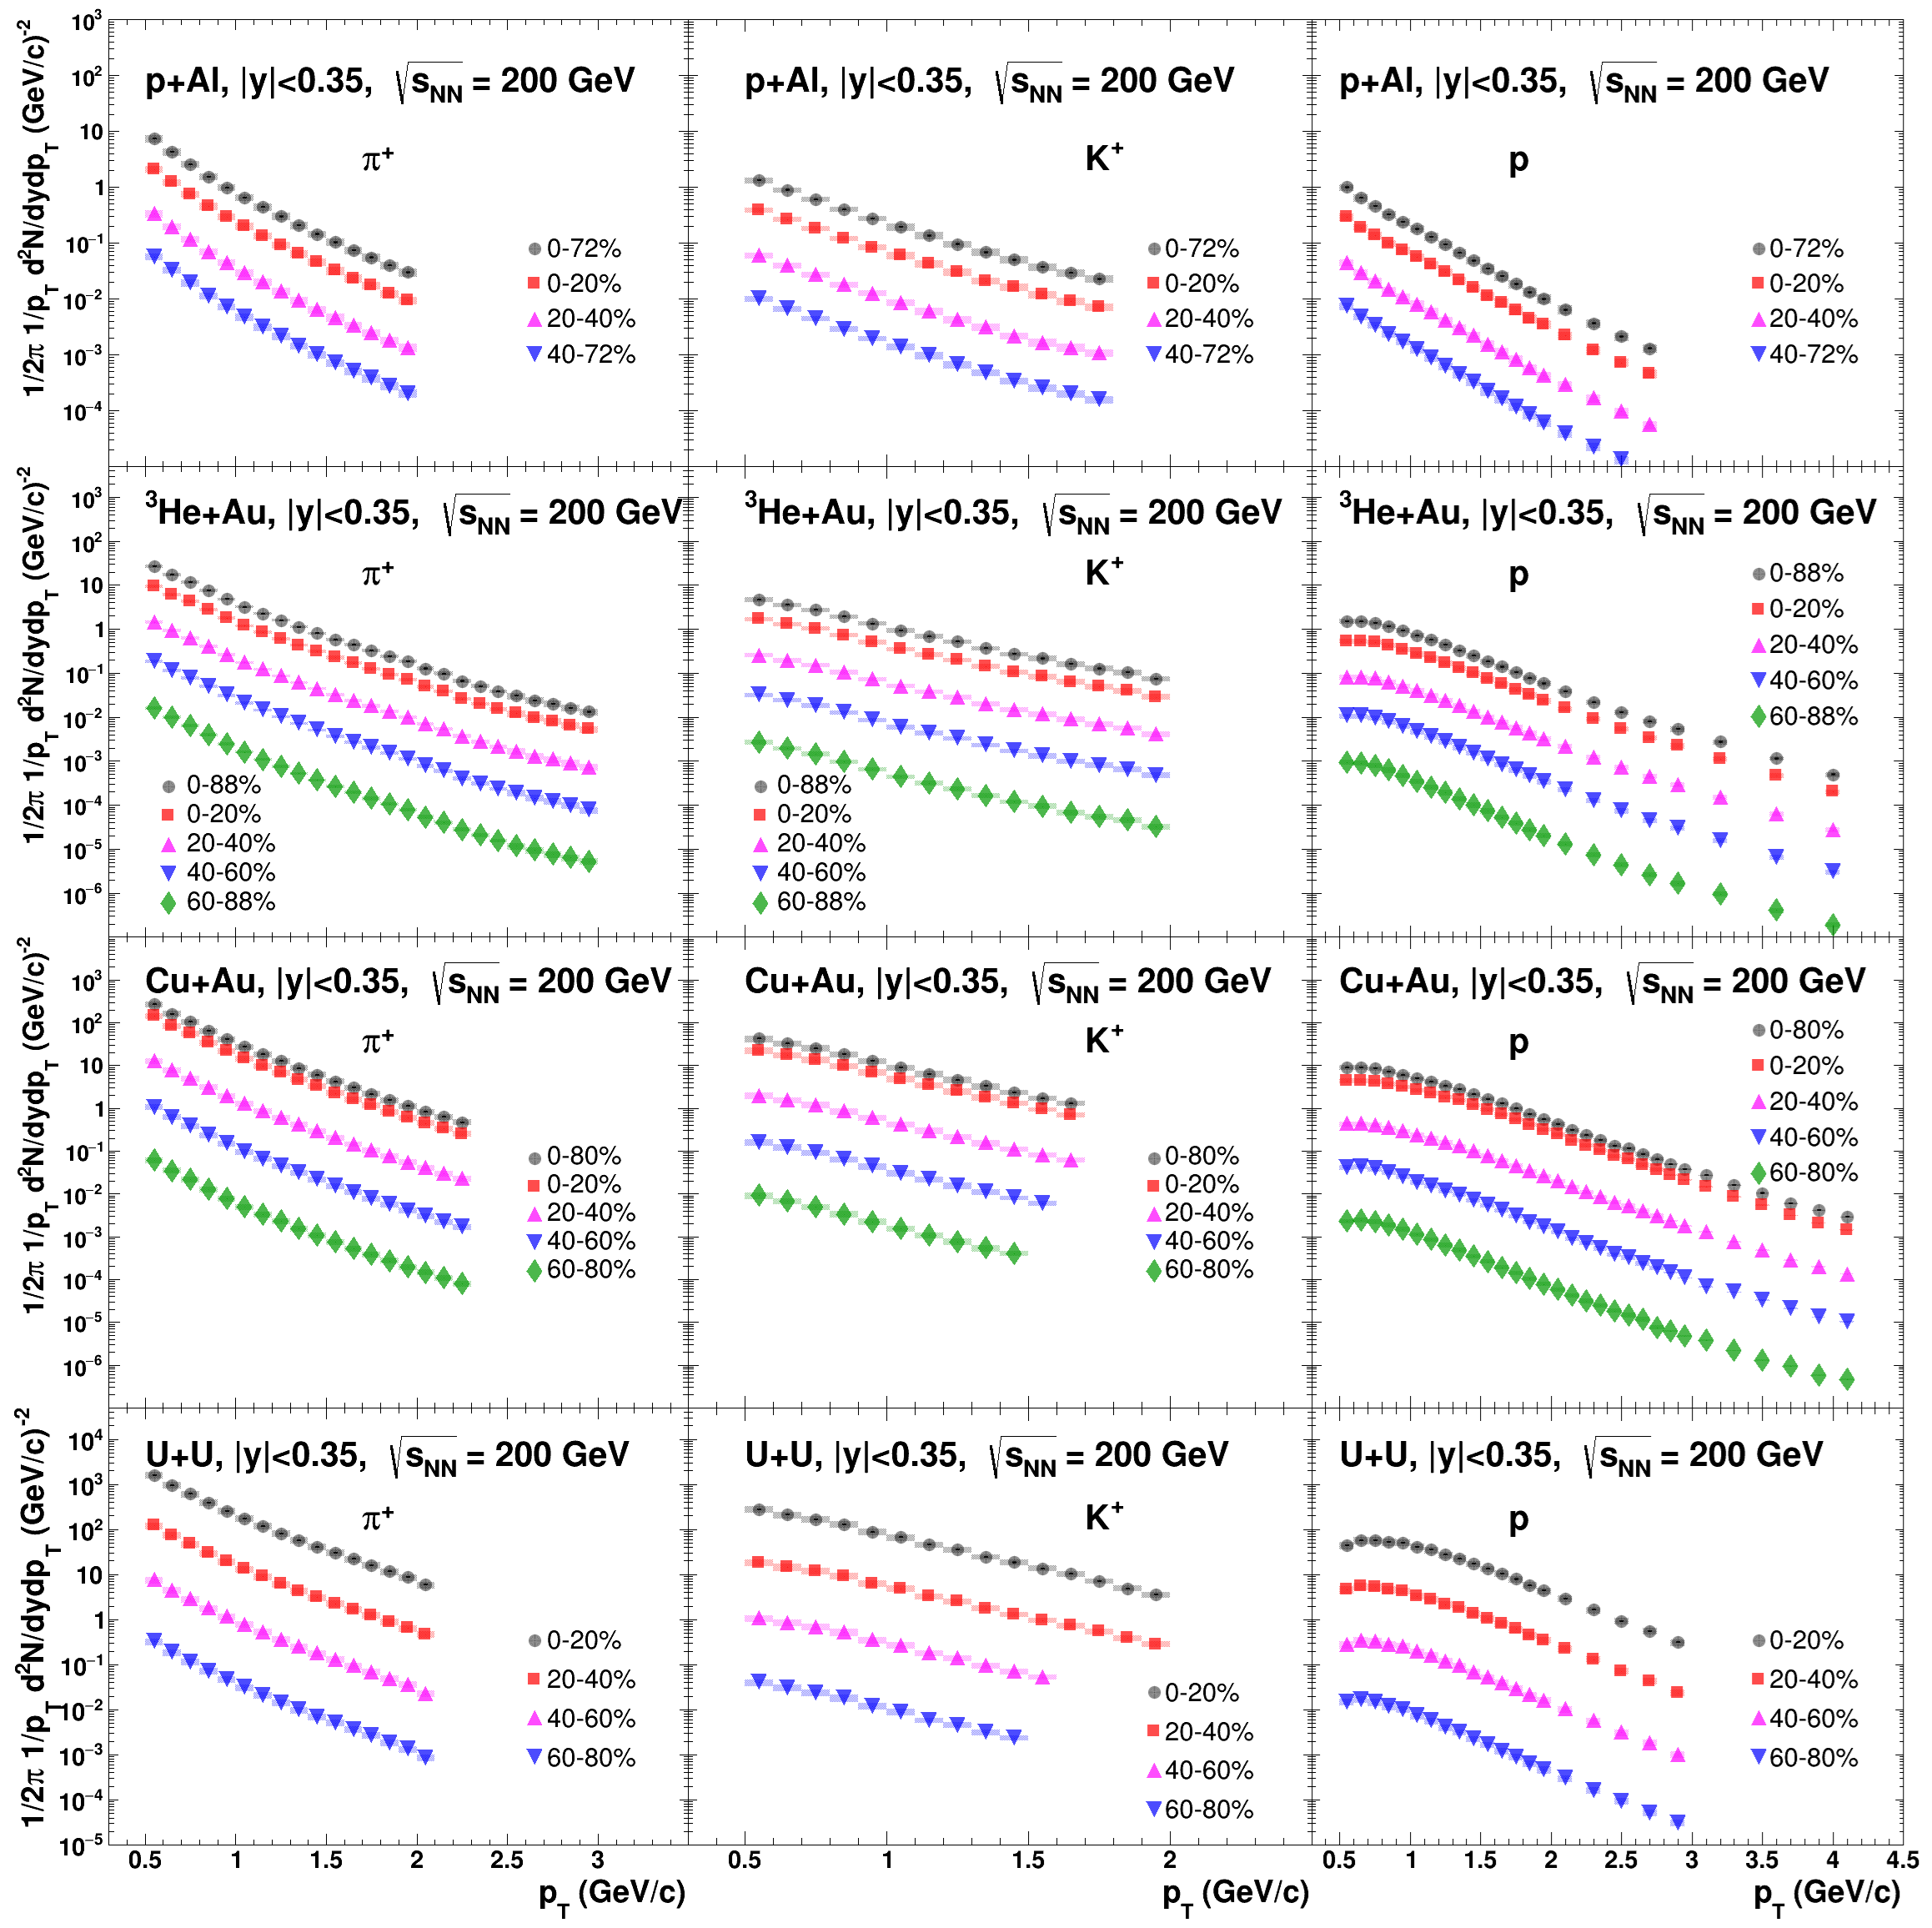
\includegraphics [width=1\linewidth]{Results/spectraDiss_pt_0.png}
	\caption{Инвариантные спектры по поперечному импульсу, измеренные для $\pi^+$, $K^+$, $p$ в различных центральностях \pal, \heau, Cu+Au и U+U столкновениях.} 
	\label{img:SpectraPt0}
\end{figure}
\begin{figure}[] 
	\centerfloat
	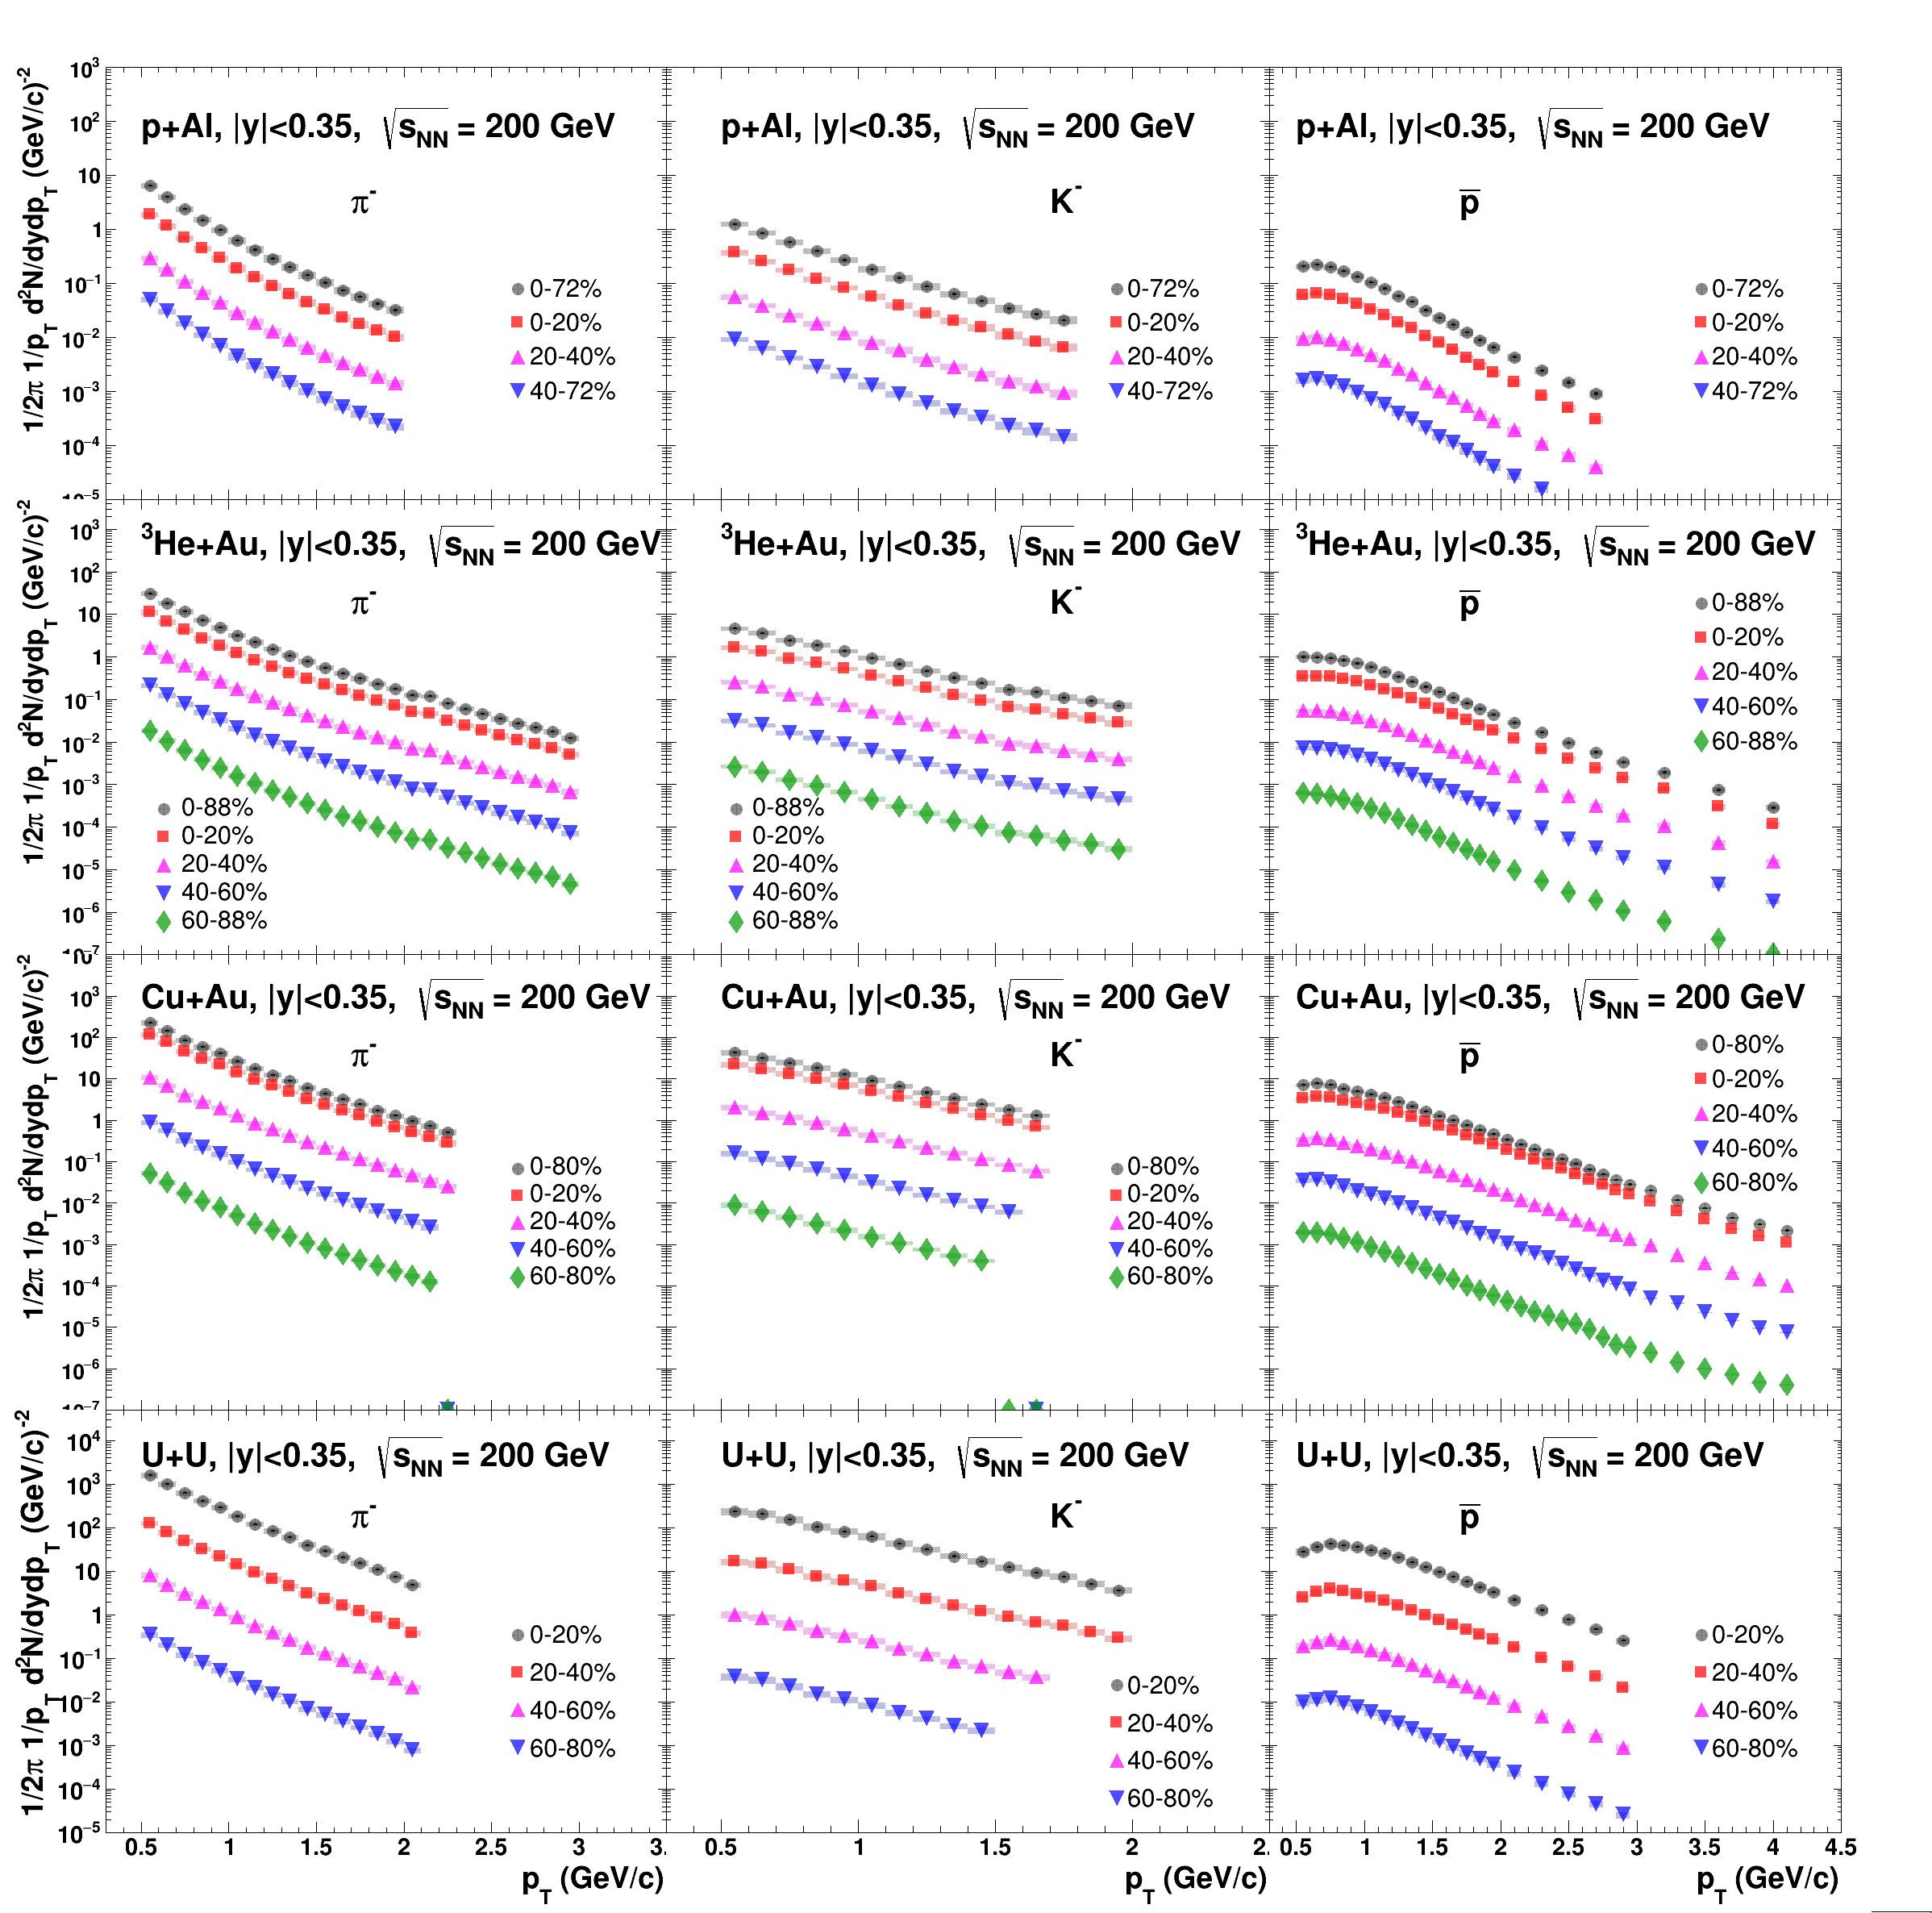
\includegraphics [width=1\linewidth]{Results/spectraDiss_pt_1.png}
	\caption{Инвариантные спектры по поперечному импульсу, измеренные для $\pi^-$, $K^-$, $\bar{p}$ в различных центральностях \pal, \heau, Cu+Au и U+U столкновениях.} 
	\label{img:SpectraPt1}
\end{figure}
\end{comment}
\begin{figure}[] 
	\centerfloat
	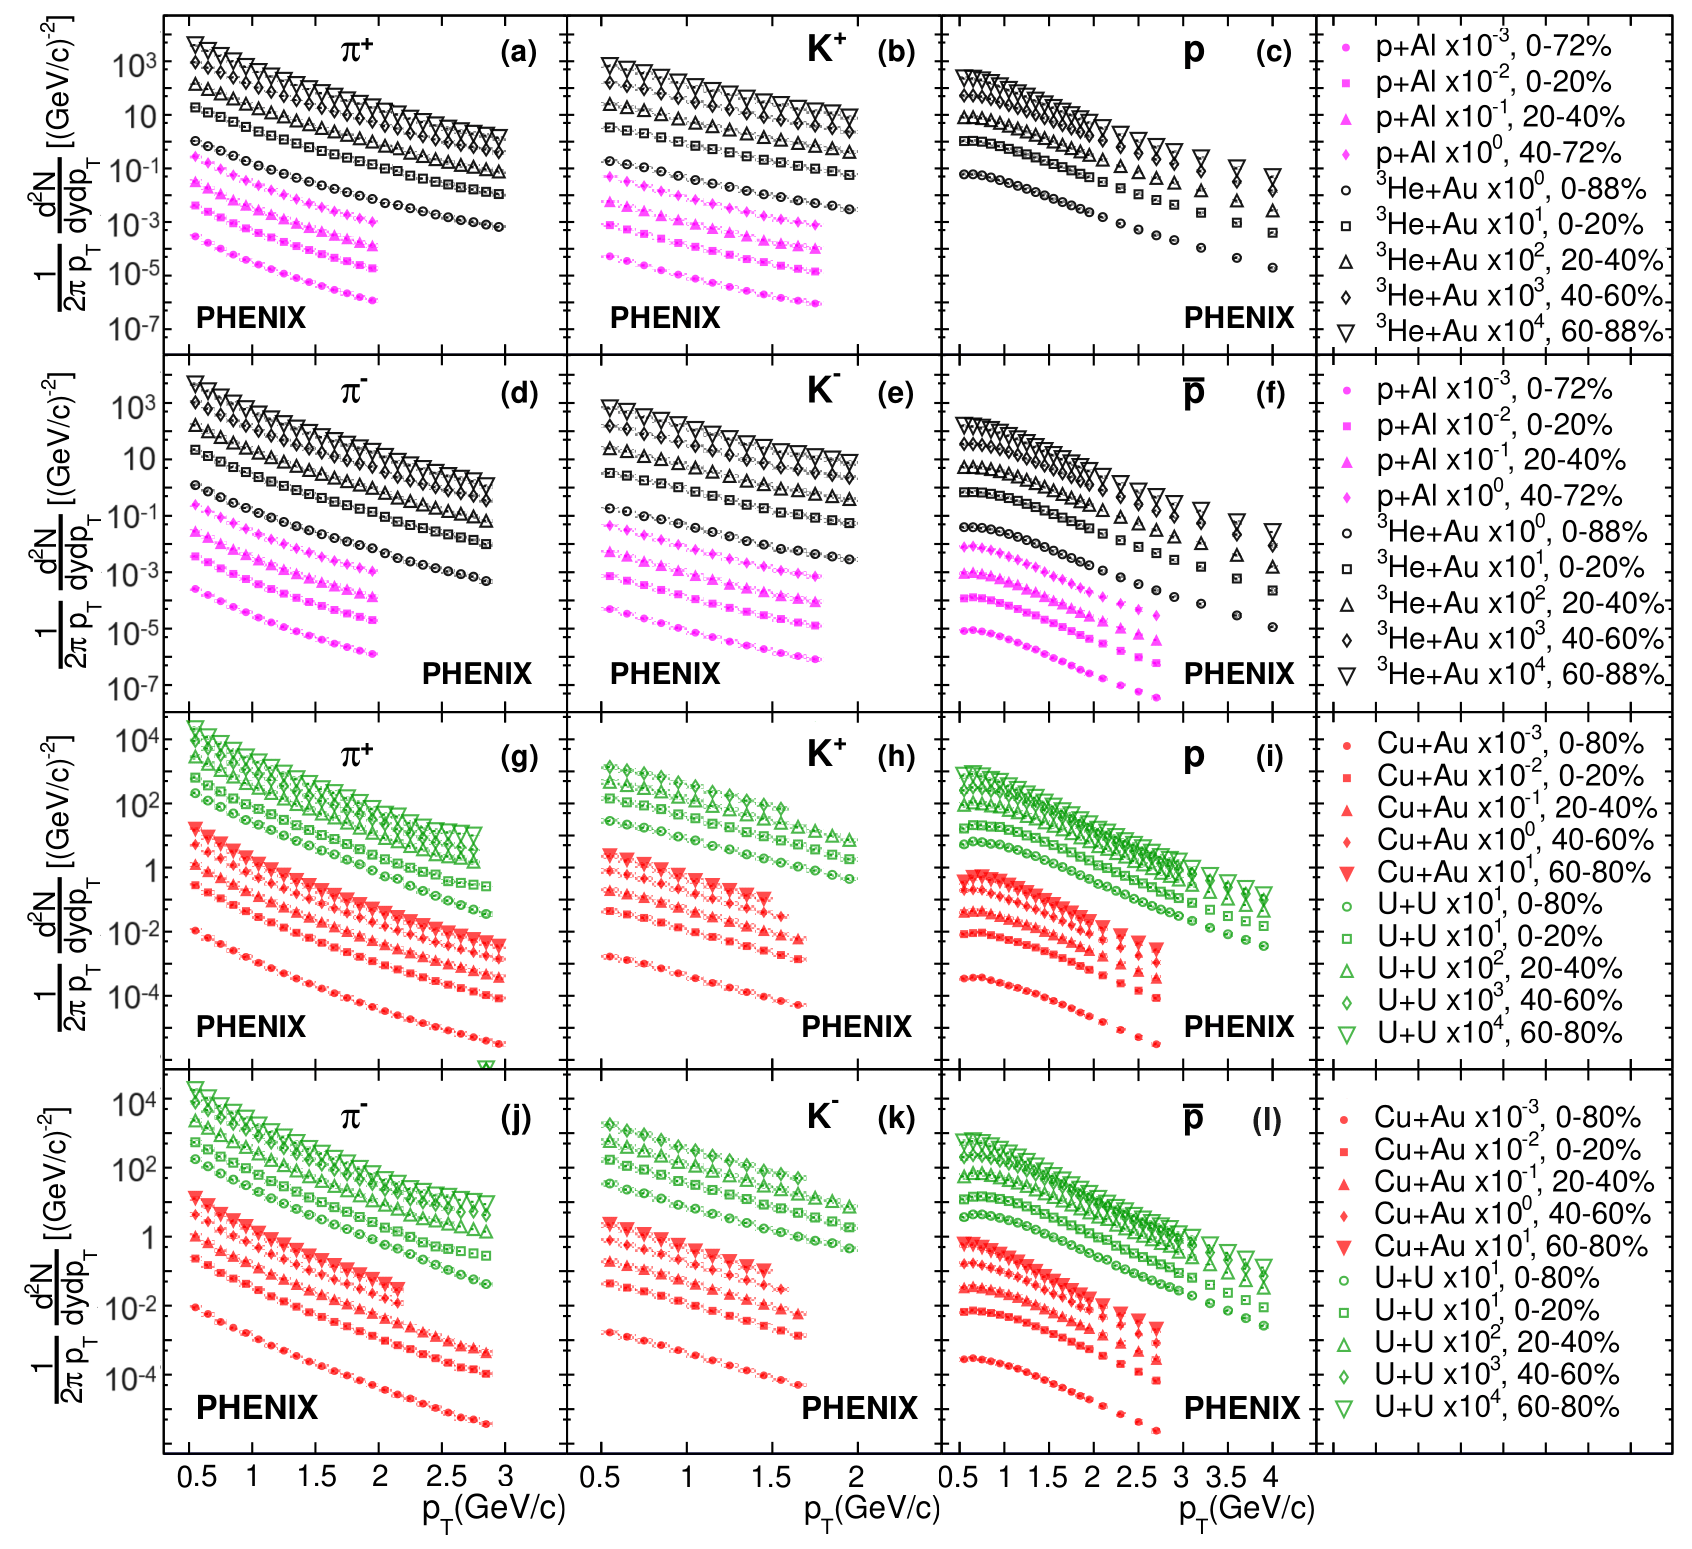
\includegraphics [width=1\linewidth]{Results/spectraOneCanvas_Pt_All.png}
	\caption{Инвариантные спектры по поперечному импульсу, измеренные для $\pi^{\pm}$, $K^{\pm}$, $p$ и $\bar{p}$ в различных центральностях \pal, \heau, Cu+Au и U+U столкновений.} 
	\label{img:SpectraPt}
\end{figure}

\section{Факторы ядерной модификации} \label{sectRes_rab}


\begin{figure}[] 
	\centerfloat
	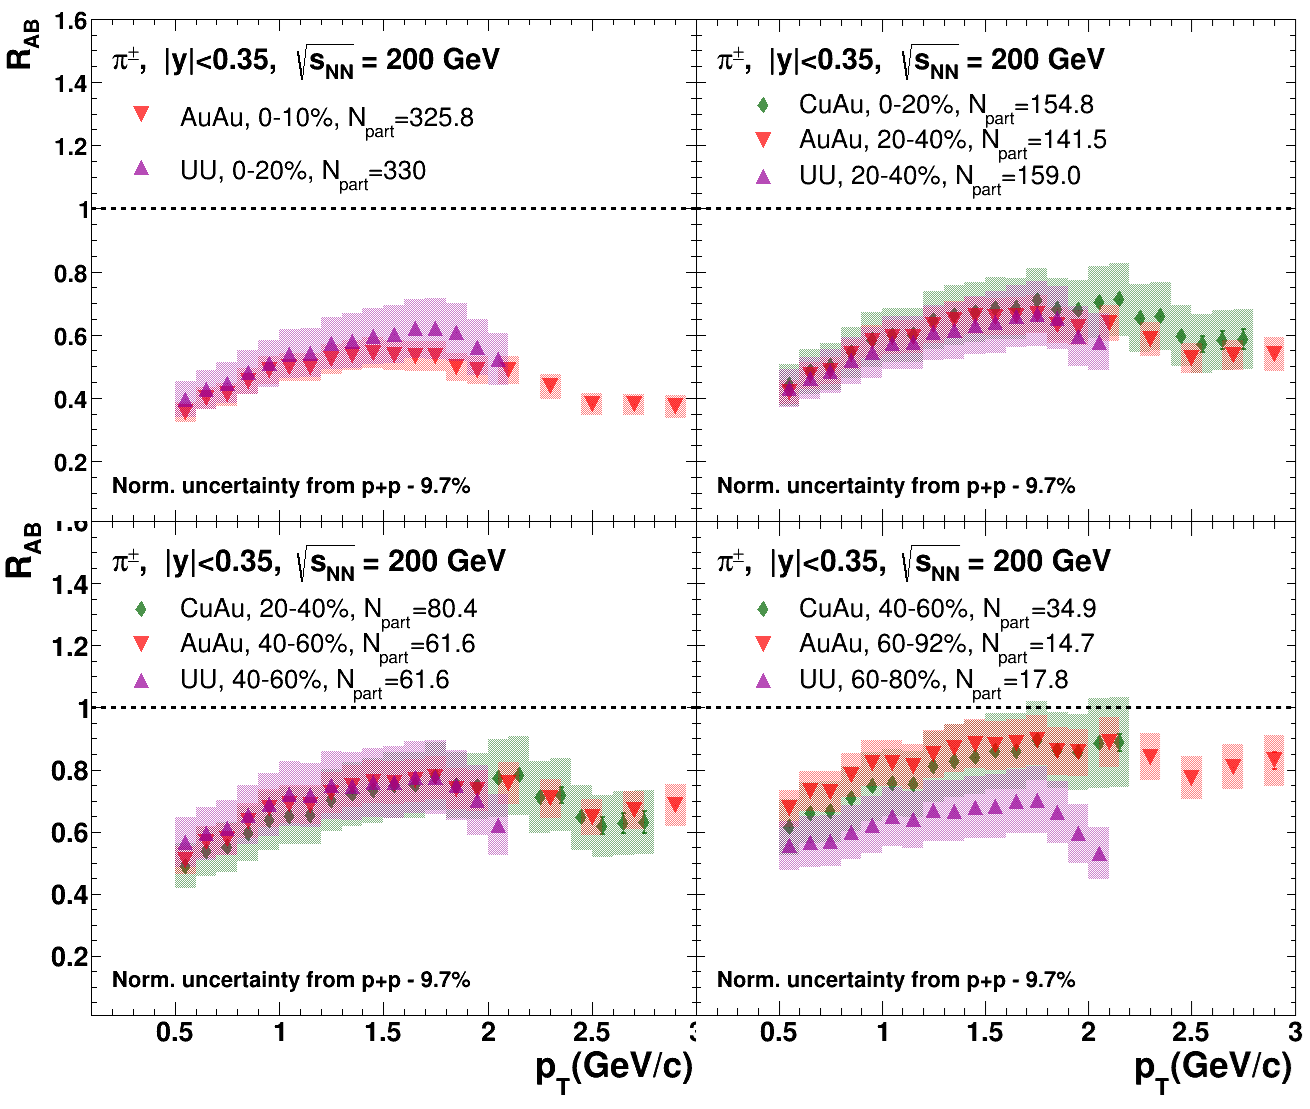
\includegraphics [width=0.7\linewidth]{Results/DrawAll_large_raa_1}
	\caption{Значения \rab, измеренные для \pipm \ в различных центральностях \cuau, \auau, \uu \ столкновений.} 
	\label{img:Res_piRab_large}
\end{figure}

\begin{figure}[] 
	\centerfloat
	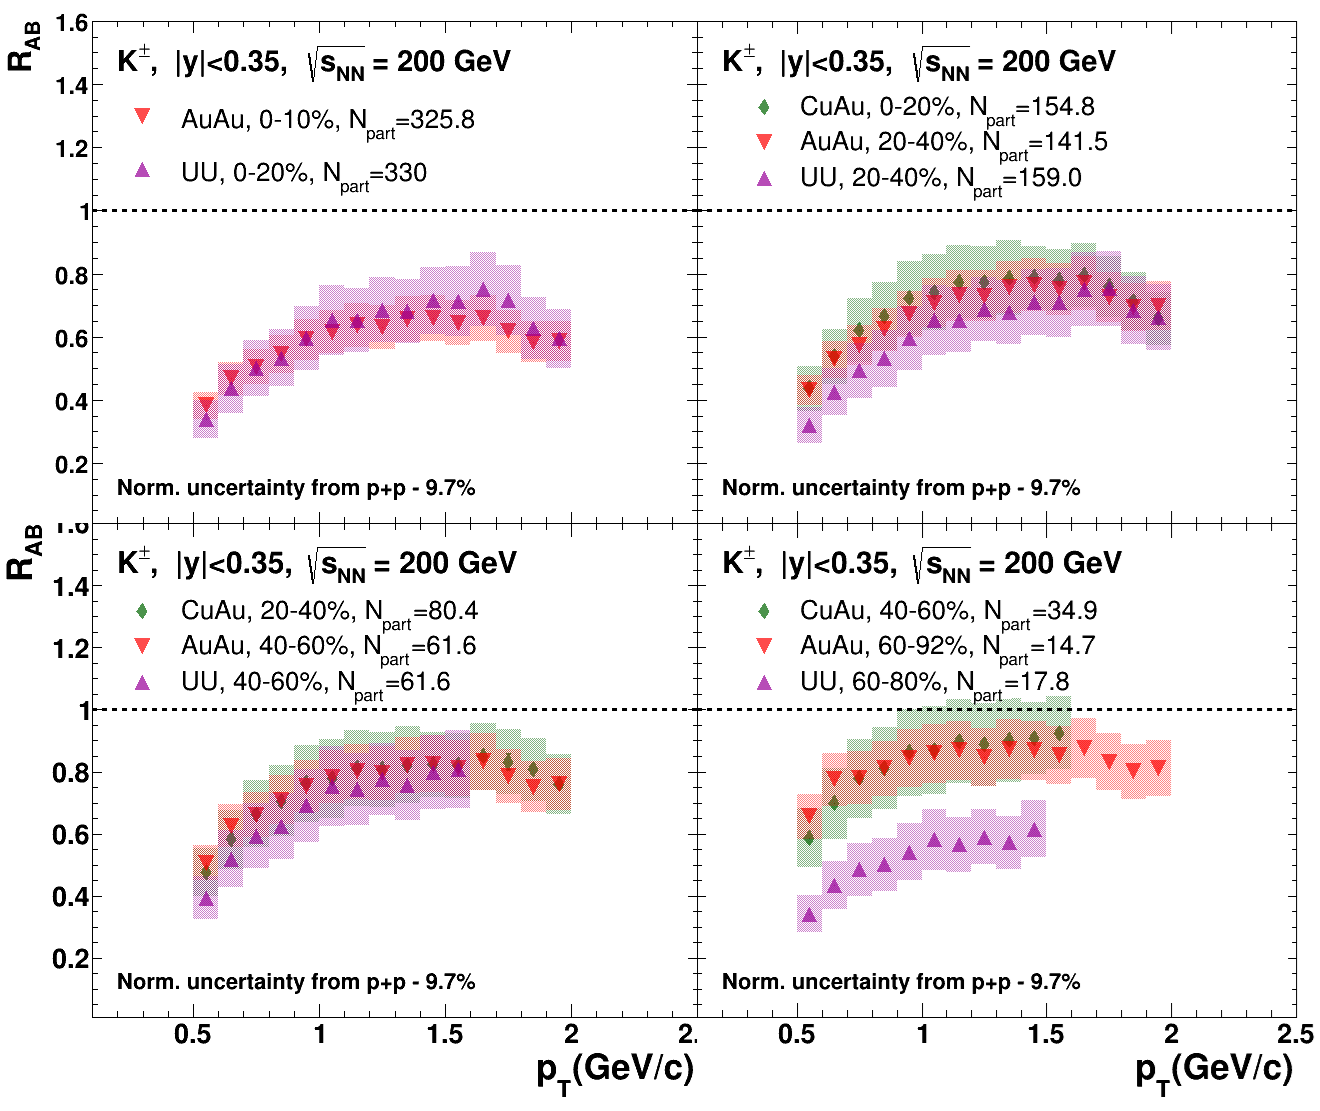
\includegraphics[width=0.7\linewidth]{Results/DrawAll_large_raa_2}
	\caption{Значения \rab, измеренные для \Kpm \ в различных центральностях \cuau, \auau, \uu \ столкновений.} 
	\label{img:Res_KRab_large}
\end{figure}

\begin{figure}[] 
	\centerfloat
	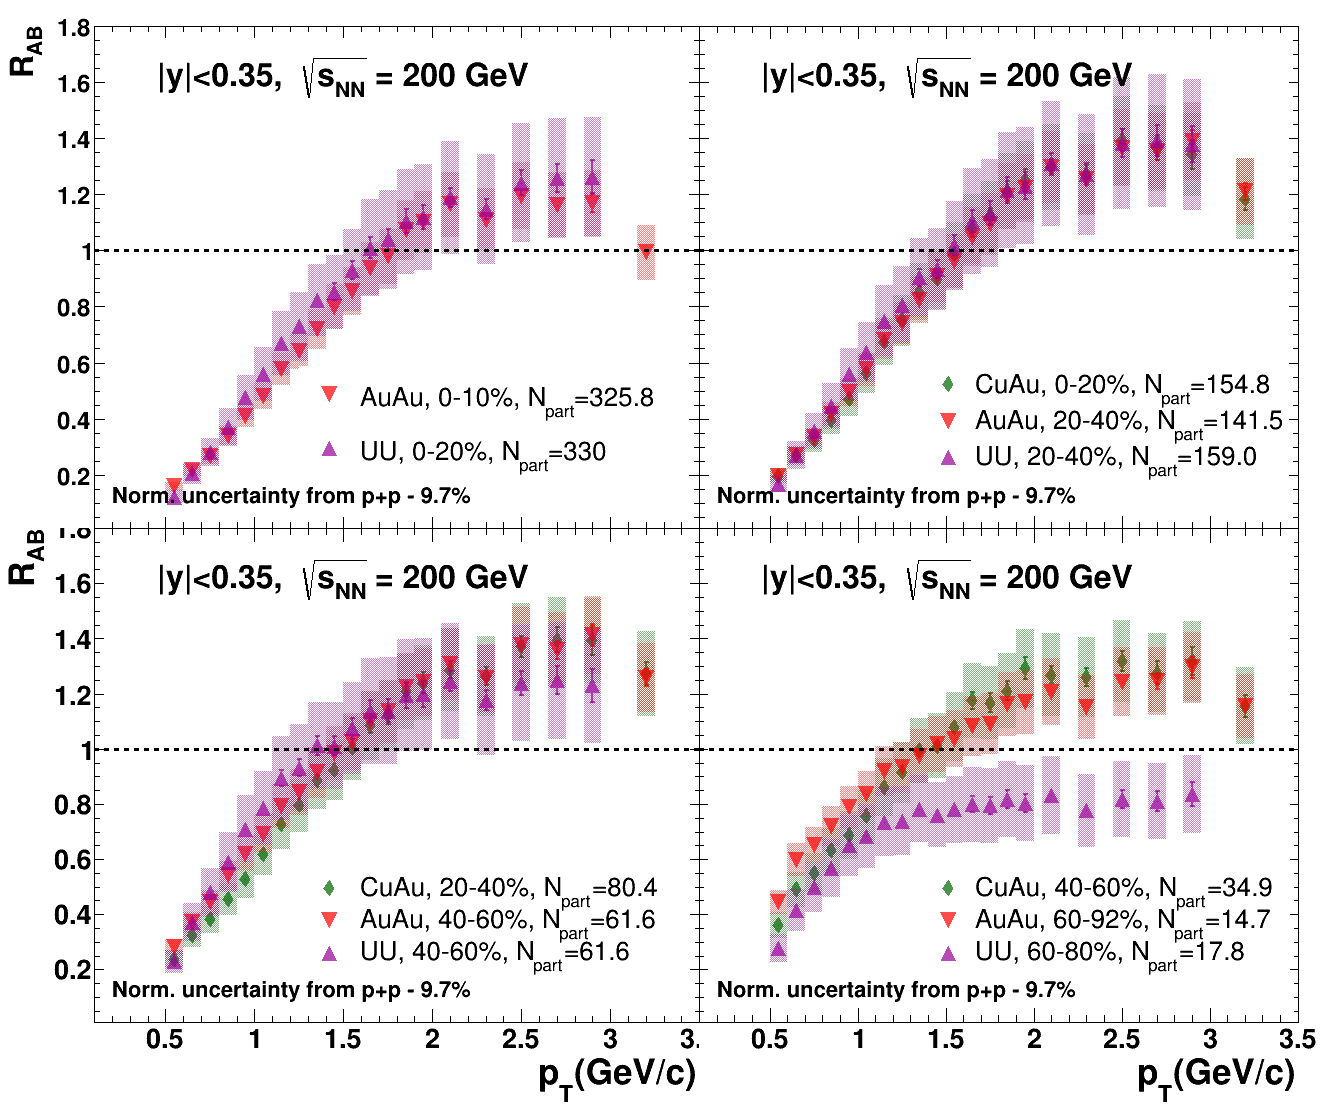
\includegraphics[width=0.7\linewidth]{Results/DrawAll_large_raa_3}
	\caption{Значения \rab, измеренные для \prots \ в различных центральностях \cuau, \auau, \uu \ столкновений.} 
	\label{img:Res_pRab_large}
\end{figure}

\begin{figure}[] 
	\centerfloat
	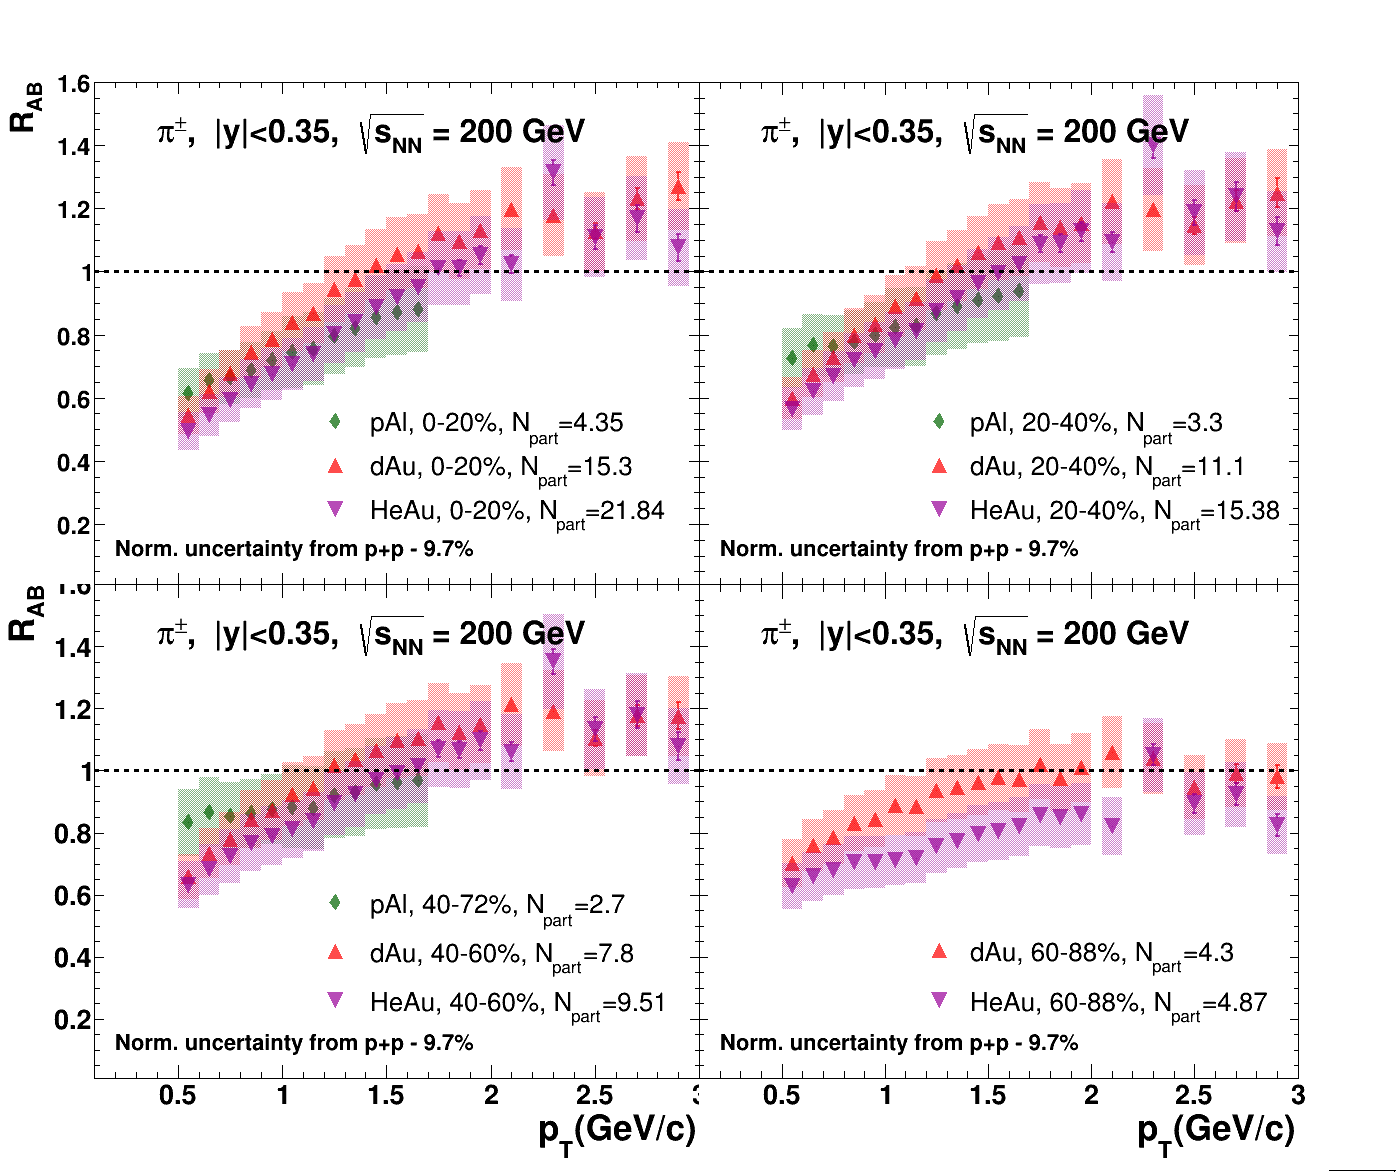
\includegraphics [width=0.7\linewidth]{Results/DrawAll_small_raa_1}
	\caption{Значения \rab, измеренные для \pipm \ в различных центральностях столкновений \pal, \heau, $d$+Au.} 
	\label{img:Res_piRab_small}
\end{figure}

\begin{figure}[] 
	\centerfloat
	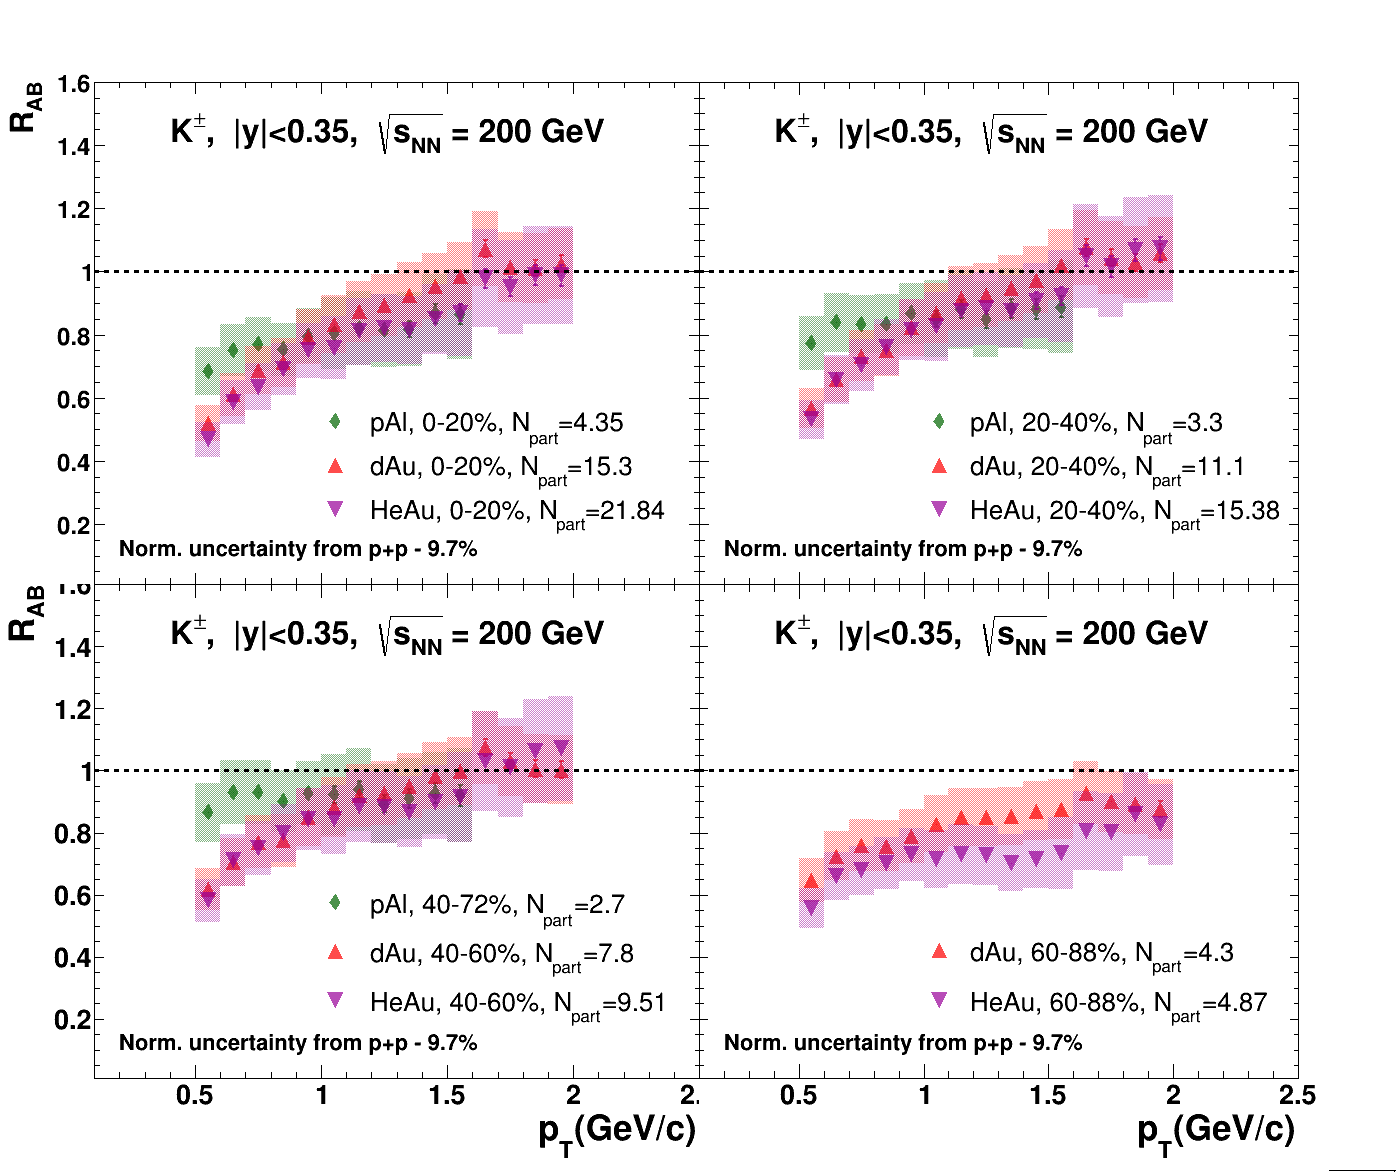
\includegraphics[width=0.7\linewidth]{Results/DrawAll_small_raa_2}
	\caption{Значения \rab \ измеренные для \Kpm \ в различных центральностях столкновений \pal, \heau, $d+Au$.} 
	\label{img:Res_KRab_small}
\end{figure}

\begin{figure}[] 
	\centerfloat
	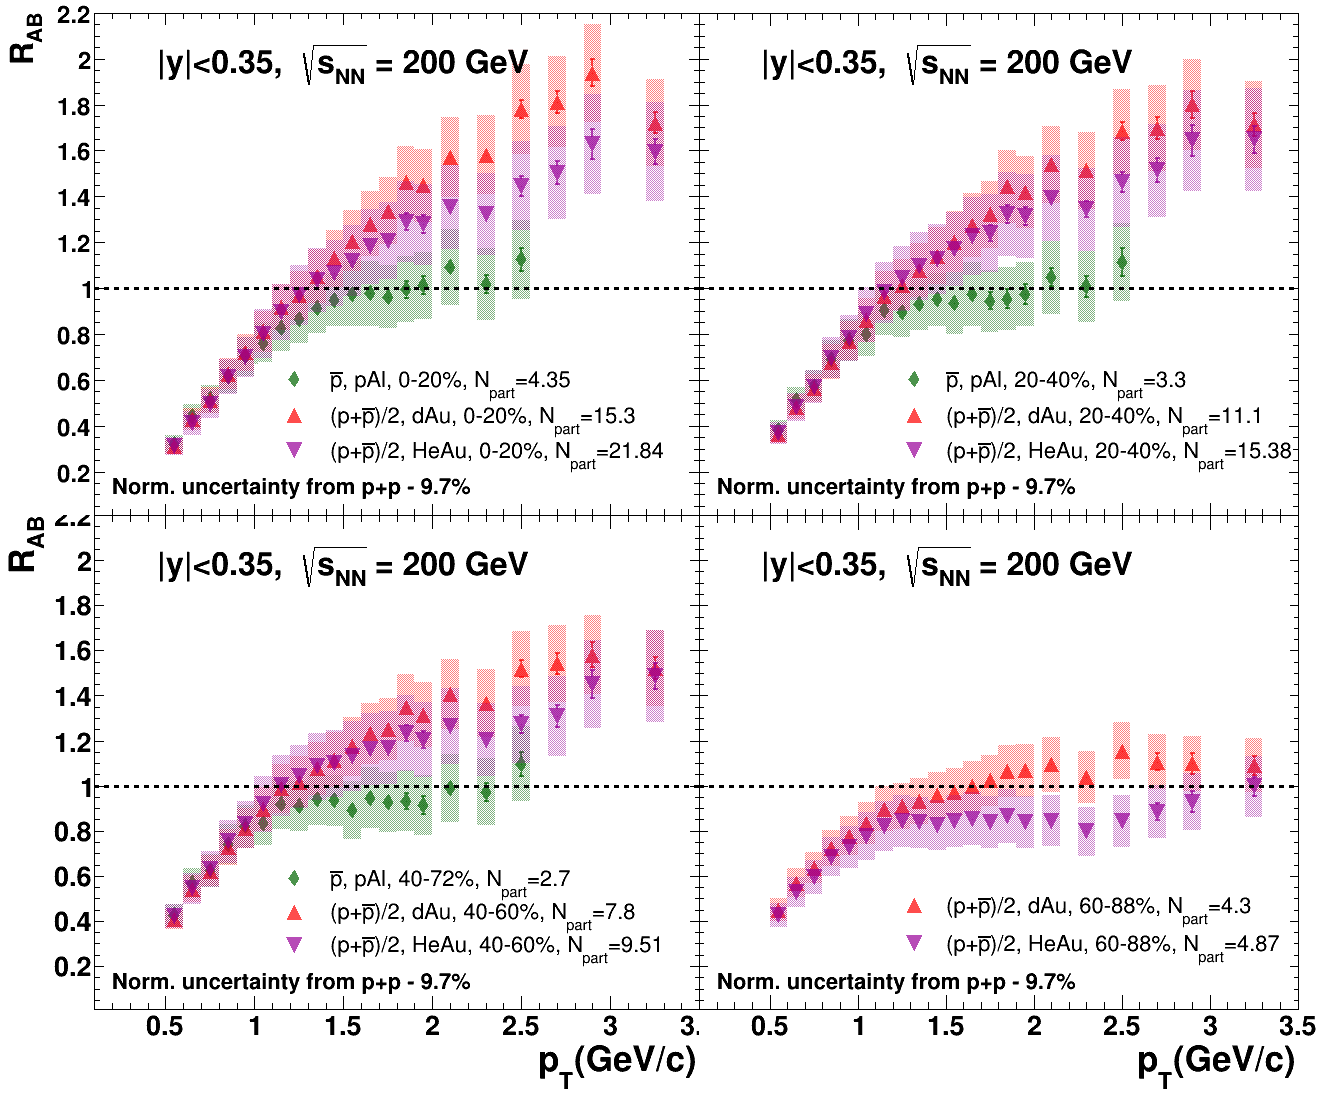
\includegraphics[width=0.7\linewidth]{Results/DrawAll_small_raa_3}
	\caption{Значения \rab \ измеренные для \aprot \ в различных центральностях столкновений \pal, и значения \rab, измеренные для \prots \ в различных центральностях \heau, $d+Au$ столкновений.} 
	\label{img:Res_pRab_small}
\end{figure}

На Рисунках \ref{img:Res_piRab_large}-\ref{img:Res_pRab_large} представлено сравнение значений \rab, измеренных для  \pipm, \Kpm-мезонов и \prots \ в \cuau \ и \auau \ столкновениях при энергии \sqsn=200 ГэВ, а также в \uu \ столкновениях при энергии \sqsn=193 ГэВ. Значения \rab, измеренные для заряженных адронов в различных системах, но при схожих значениях количества нуклонов-участников (\Npart), совпадают в пределах систематических неопределенностей. Данный результат может означать, что рождение заряженных адронов зависит от размера области перекрытия сталкивающихся ядер, но не зависит от ее формы.

\newpage
На Рисунках \ref{img:Res_piRab_small}-\ref{img:Res_pRab_small} представлено сравнение значений \rab, измеренных для  \pipm, \Kpm-мезонов и \aprot \ в \pal \ столкновениях, и значений \rab, измеренных для \pipm, \Kpm-мезонов и \prots \ в \dau \ и \heau \ столкновениях при энергии \sqsn=200 ГэВ. Значения \rab, измеренные для \pipm, \Kpm-мезонов в различных системах, но при схожих значениях \Npart, совпадают в пределах погрешностей. Значения \rab, измеренные для \aprot \ в \pal \ столкновениях, близки к единице и меньше значений \rab, измеренных для \prots \ в \heau \ и \dau \ столкновениях. Также важно отметить, что зависимость значений \rab \ от \pt, измеренных для \pipm \ и \Kpm-мезонов в \pal \ столкновениях, имеет меньший наклон, чем наклон зависимостей значений \rab \ от \pt, измеренных для \pipm, \Kpm-мезонов в \dau \ и \heau \ столкновениях. 

\subsubsection{Сравнение факторов ядерной модификации легких адронов}
На Рисунке \ref{img:Res_HadronRab_large} показаны факторы ядерной модификации легких адронов в столкновениях тяжелых систем при энергии \sqsn=200 ГэВ. В центральных столкновениях значения протонных \rab \ превышают значения \rab, измеренные для мезонов, в промежуточном диапазоне \pt \ (1 ГэВ/$c$ $< p_T <$ 4 ГэВ/с). В частности, значения \rab, измеренные для протонов, больше, чем значения \rab, измеренные для $\phi$-мезонов. Принимая во внимание, что масса $\phi$-мезона $m_{\phi}$=1,019 ГэВ/$c^{2}$ сравнима c массой протона, можно сделать вывод, что разница значений \rab \ не может быть объяснена зависимостью от массы частицы.  

%Увеличенный по сравнению с $p+p$ столкновениями выход протонов считается одним из характерных признаков образования КГП \cite{BaryonPuzzleVelkovska, BaryonPuzzle2002, BaryonPuzzleHeavy}.

Также в центральных столкновениях важно отметить совпадение значений \rab \ мезонов, содержащих странные кварки, таких как \Kstar, \phim \ и \Kpm. Значения \rab \ таких мезонов близки к единице. Значения \rab \ мезонов, которые не содержат странных кварков, таких как \pio \ и \pipm,  также совпадают между собой в промежуточном диапазоне \pt, однако имеют меньшие величины по сравнению с мезонами, содержащими странный кварк. Данная закономерность может указывать на эффект увеличения выхода странности, являющимся одним из основных признаков образования КГП \cite{Strangeness_QGP, StrangEnh, ThermalStrangeness}.

\begin{figure}[] 
	\centerfloat
	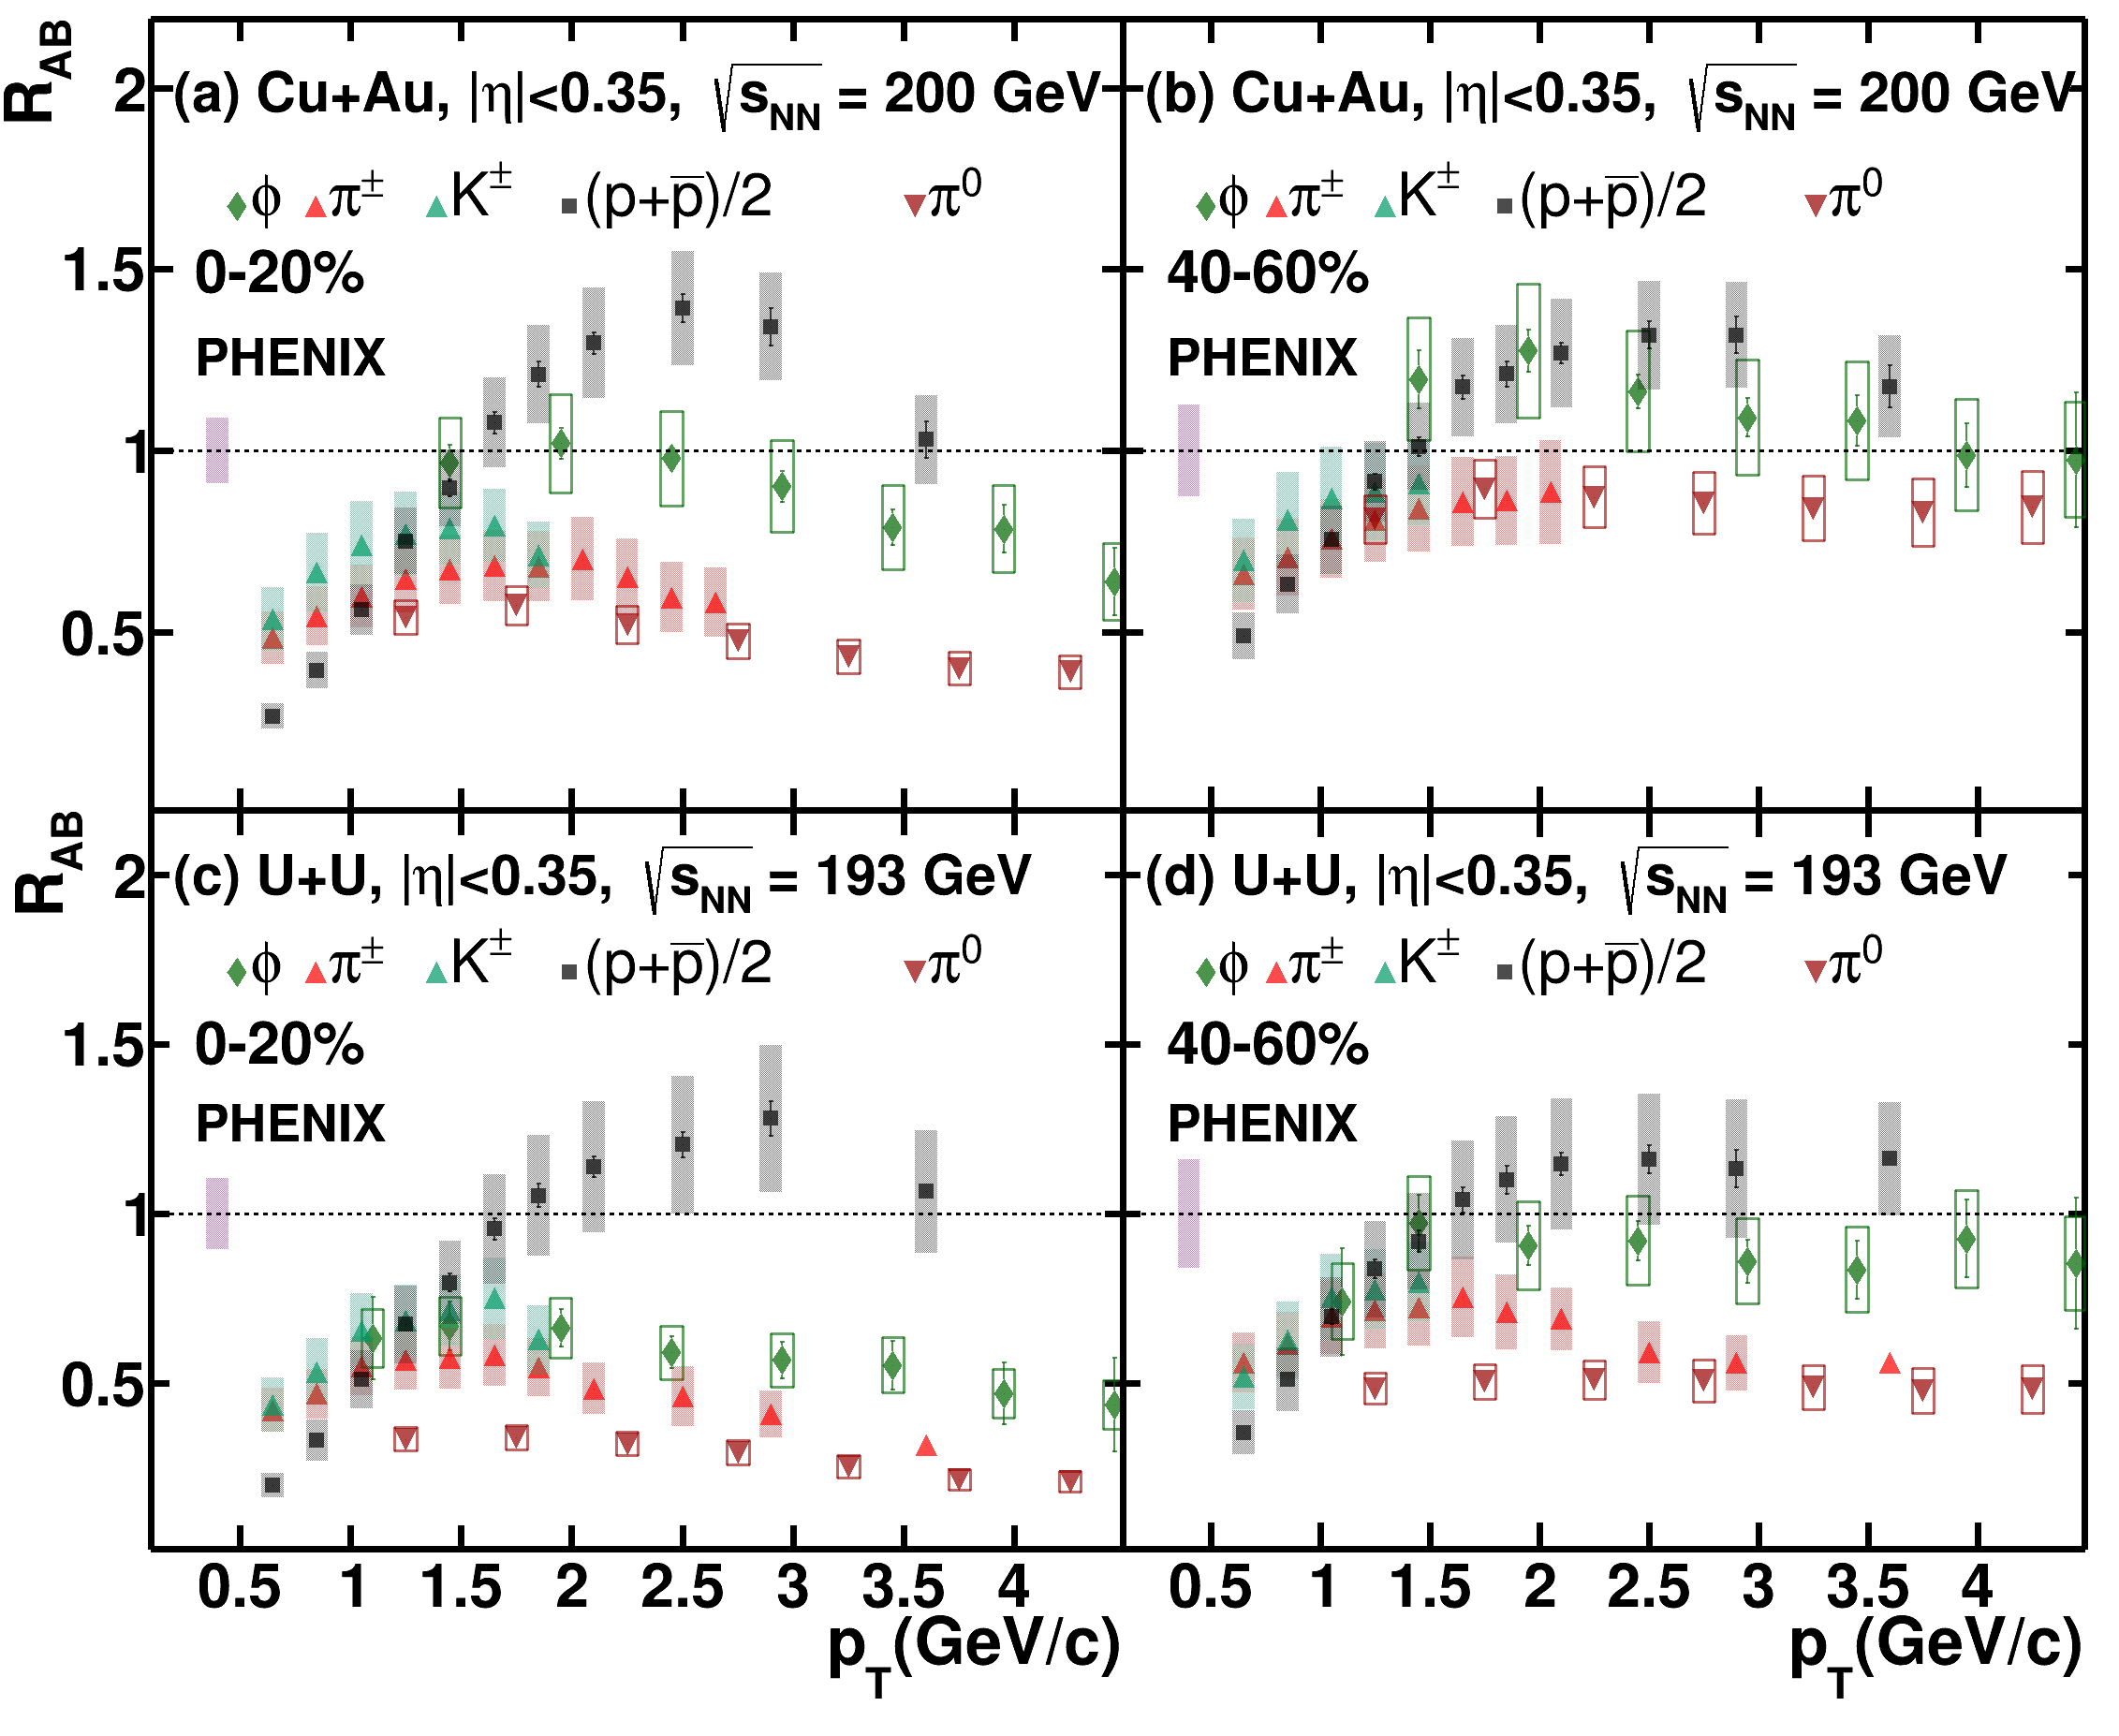
\includegraphics [width=0.65\linewidth]{Results/DrawMesons_large}
	\caption{Значения \rab, измеренные для легких адронов (\pipm, \pio, \Kpm, $\varphi$, \prots) в центральных и периферических столкновениях \cuau и \uu.} 
	\label{img:Res_HadronRab_large}
\end{figure}

На Рисунке \ref{img:Res_HadronRab_small} представлены значения \rab, измеренные для различных легких адронов (\pipm, \pio, \Kstar, \Kpm, $\varphi$, \prots) в легких системах столкновений (\pal \ и \heau).
Значения \rab \ всех рассматриваемых мезонов совпадают в пределах погрешностей как в центральных, так и в периферийных столкновениях \pal \ и \heau. В частности, значения \rab, измеренные для мезонов, содержащих странный кварк (\phim, \Kpm, \Kstar) совпадают в пределах систематических неопределенностей со значениями \rab, измеренными для мезонов, не содержащих странный кварк (\pipm, \pio). Таким образом в столкновениях \pal \ и \heau \ не наблюдается увеличенный выход странности. 
Увеличенный по сравнению с $p+p$ столкновениями (\rab > 1) выход протонов наблюдается только в центральных столкновениях \heau. В  \pal \ столкновениях и периферийных столкновениях \heau \ значения \rab \ протонов совпадают со значениями \rab \ мезонов в пределах систематических неопределенностей.  

\begin{figure}[] 
	\centerfloat
	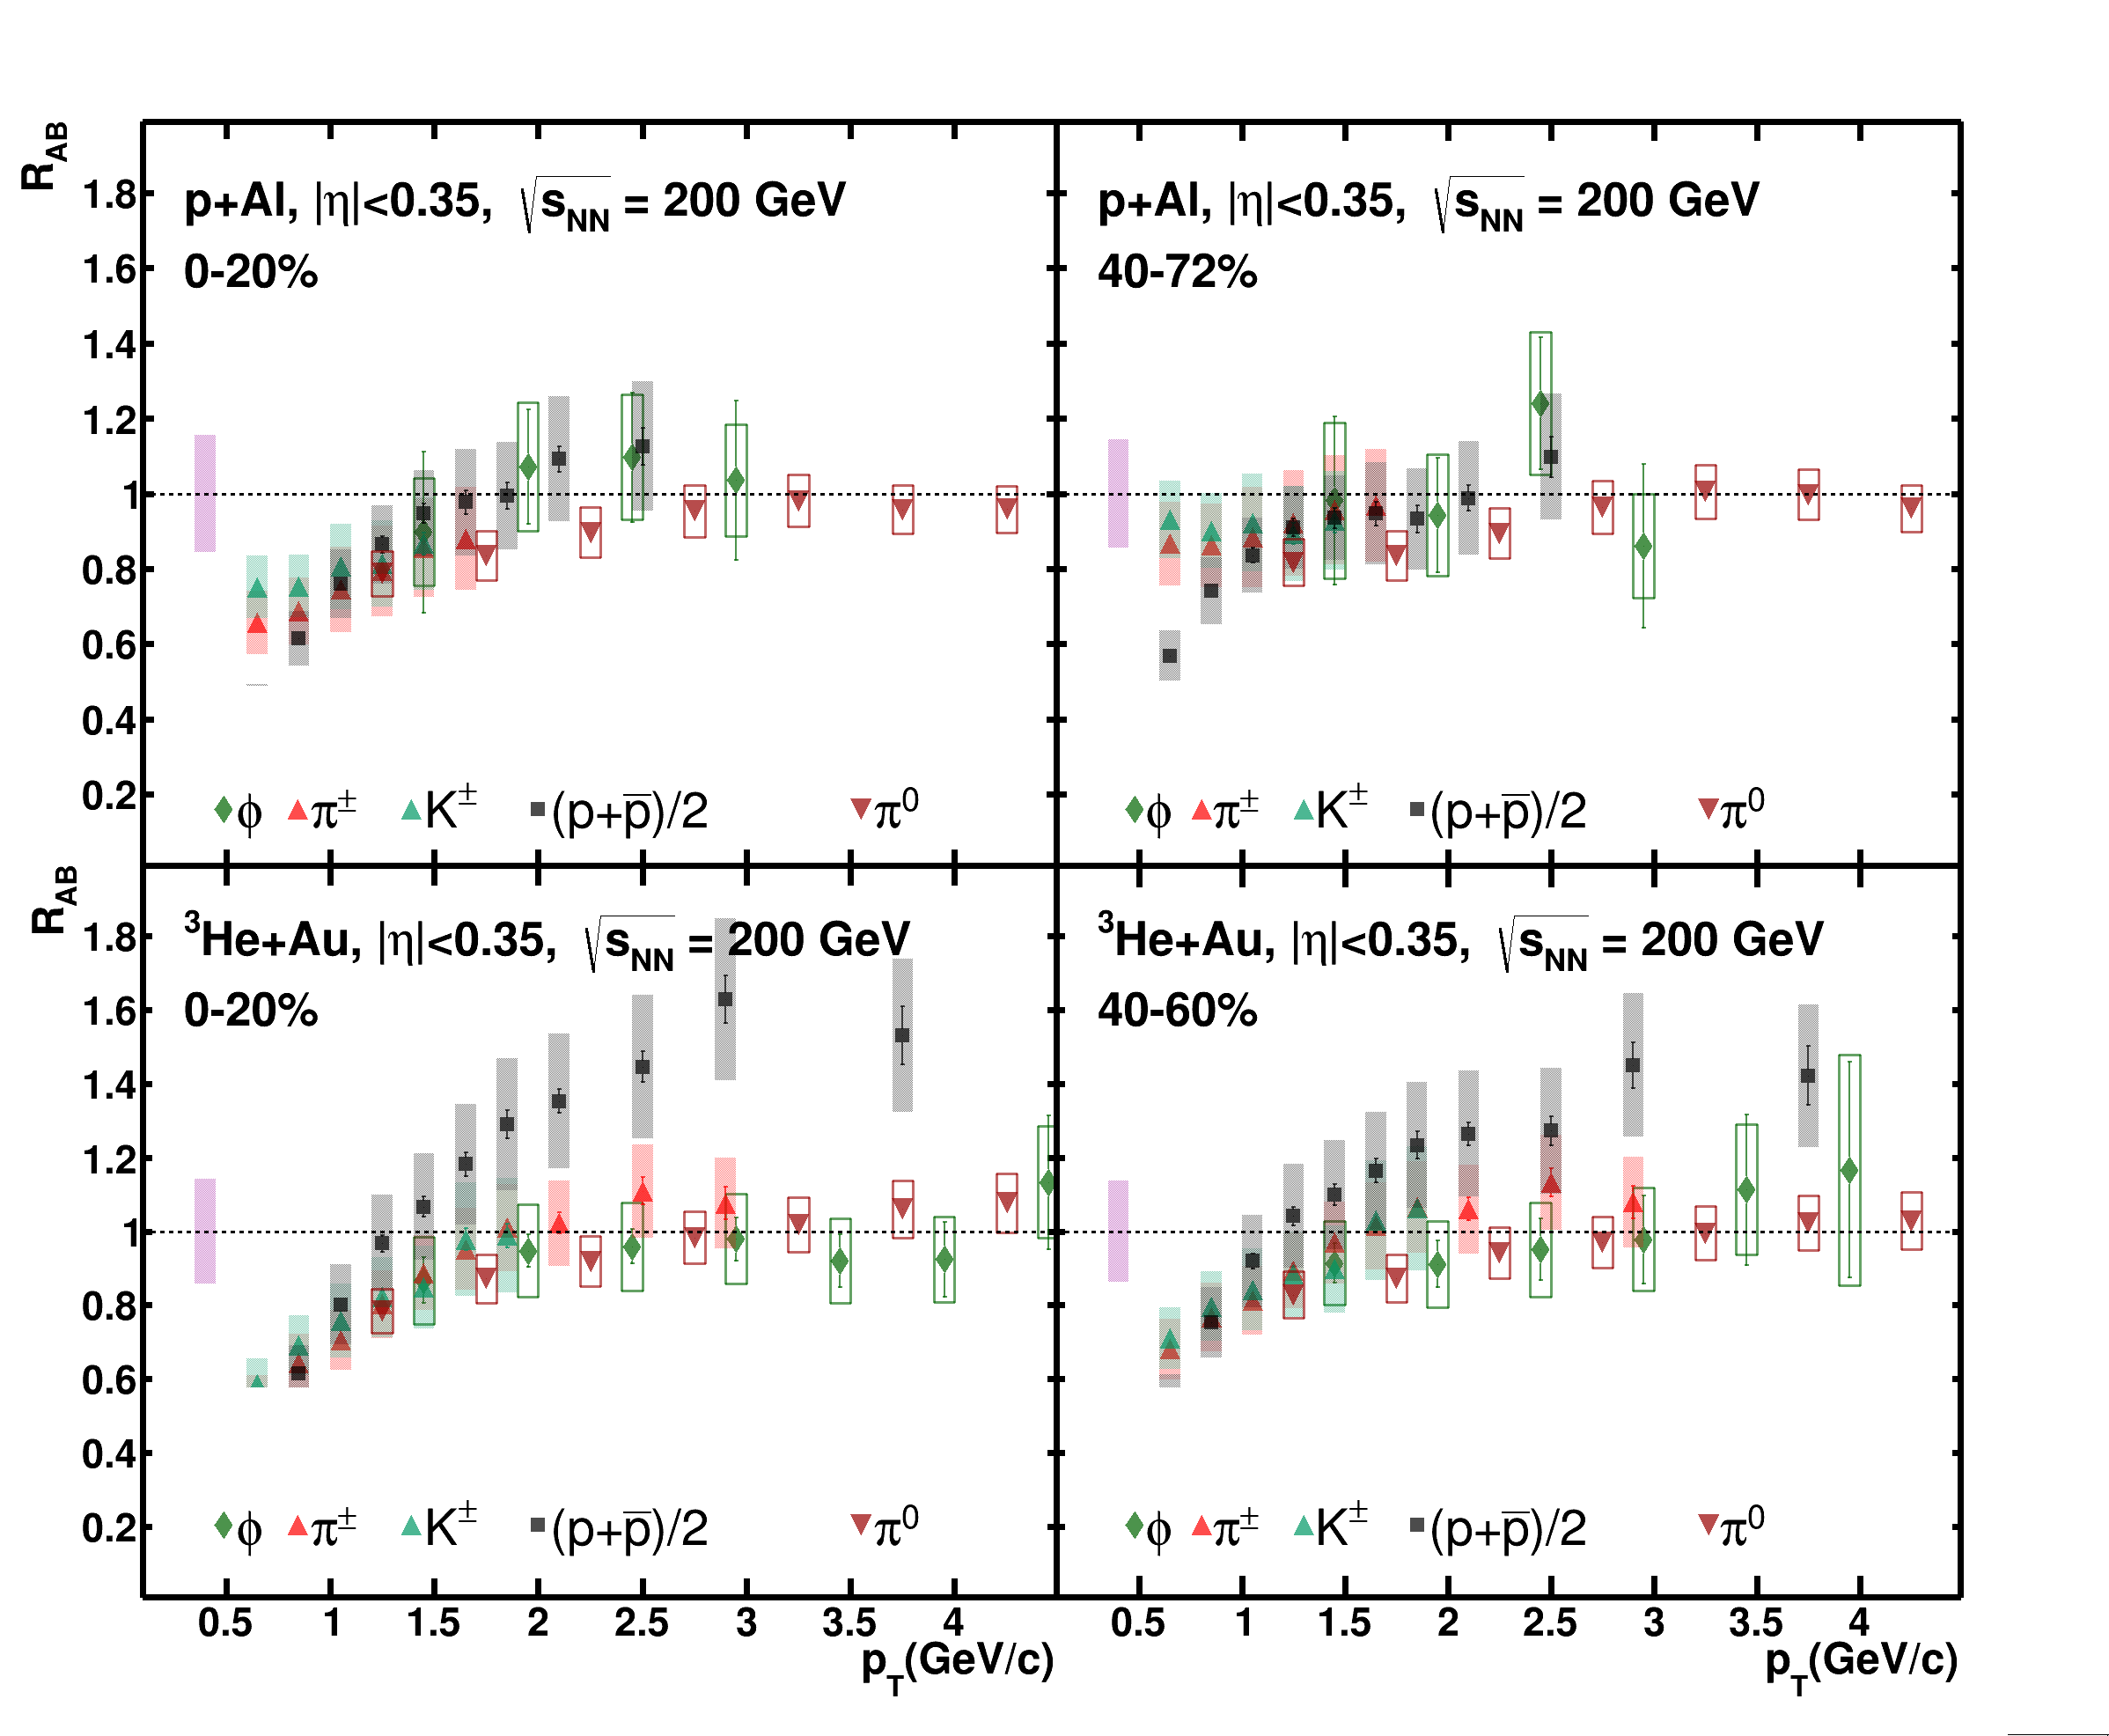
\includegraphics [width=0.65\linewidth]{Results/DrawMesons_small}
	\caption{Значения \rab, измеренные для легких адронов (\pipm,\pio,\Kpm,\phim,\prots) в центральных и периферических столкновениях \pal и \heau} 
	\label{img:Res_HadronRab_small}
\end{figure}


\section{Отношения выходов \ratppi~ и \ratKpi}
С целью более детального изучения различий в процессах образования протонов и мезонов были вычислены следующие отношения инвариантных спектров частиц: $p/\pi^{+}$, $\bar{p}/\pi^{-}$, $K^{+}/\pi^{+}$, $K^{-}/\pi^{-}$.


%\begin{equation}
	%\label{eq:ratios}
	%p/\pi = \frac{(d^2 N_p)/(dp_T dy)}{(d^2 N_{\pi})(d p_T dy)}    
%\end{equation}

\begin{figure}[] 
	\centerfloat
	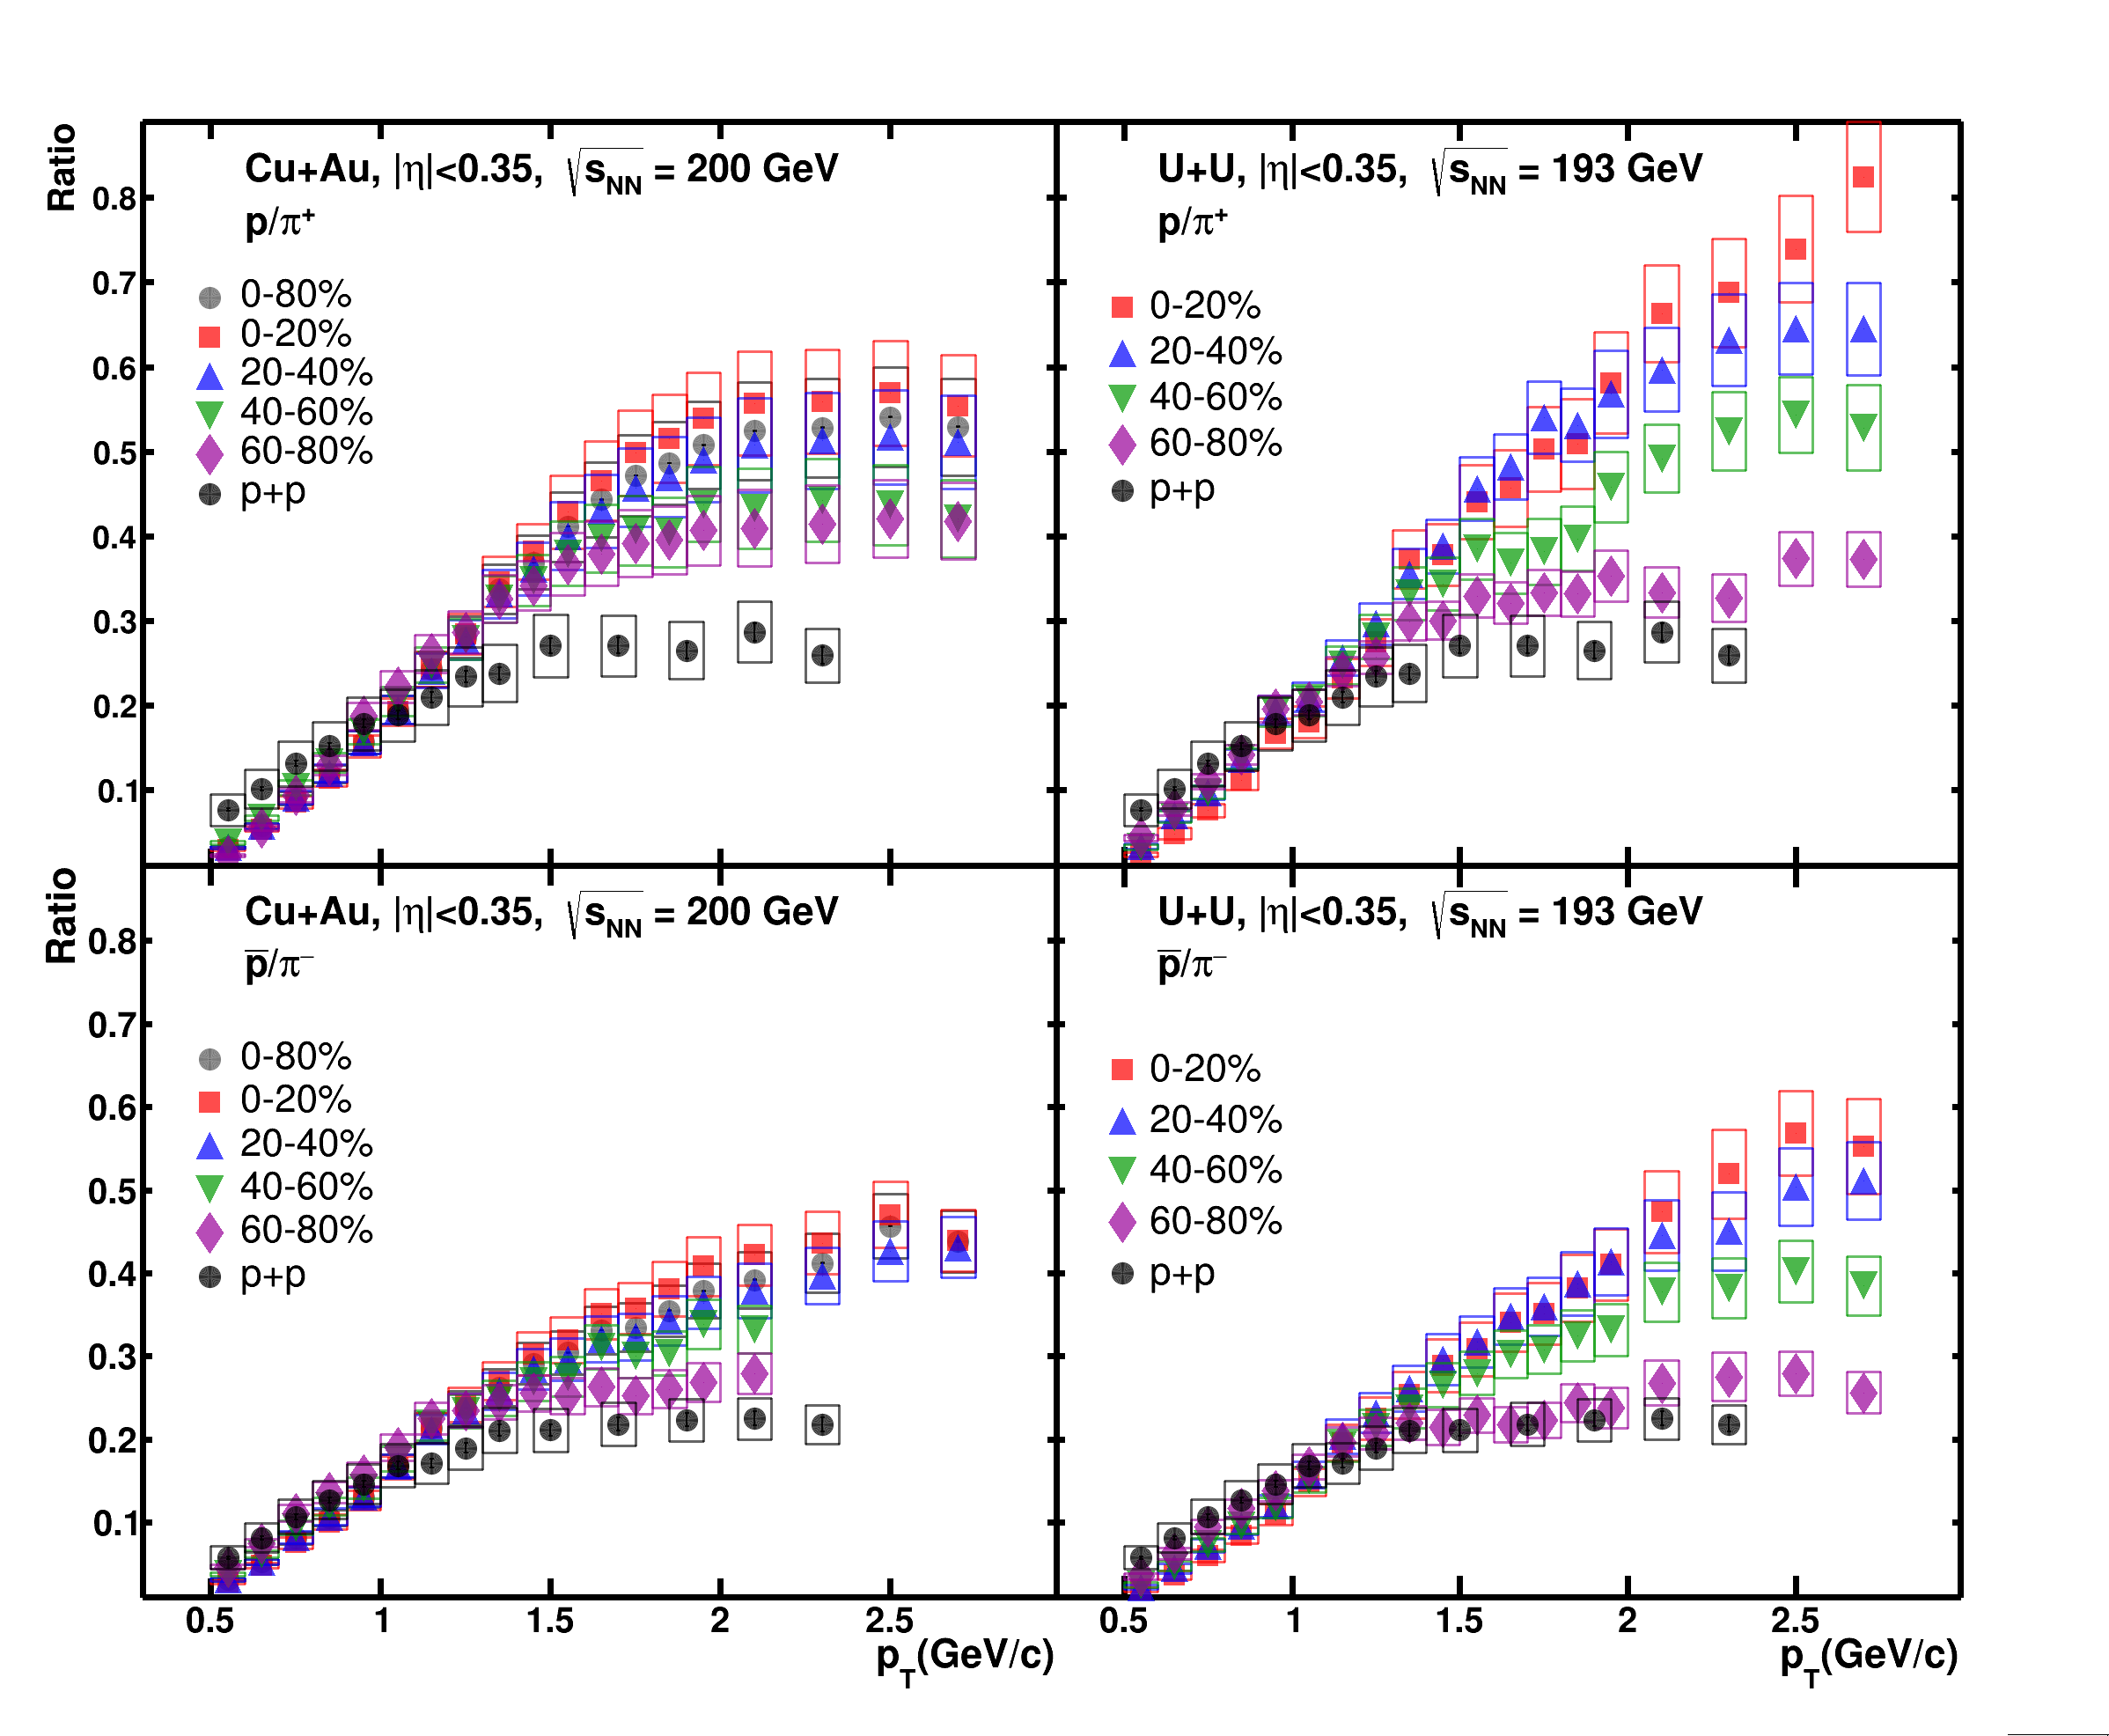
\includegraphics [width=0.7\linewidth]{Results/InOneCanvasHmy_large_p2pi}
	\caption{Значения отношений \ratppi, измеренные в различных центральностях \cuau \ и \uu \ столкновений.} 
	\label{img:Res_p2pi_large}
	
\end{figure}

\begin{figure}[] 
	
	\centerfloat
	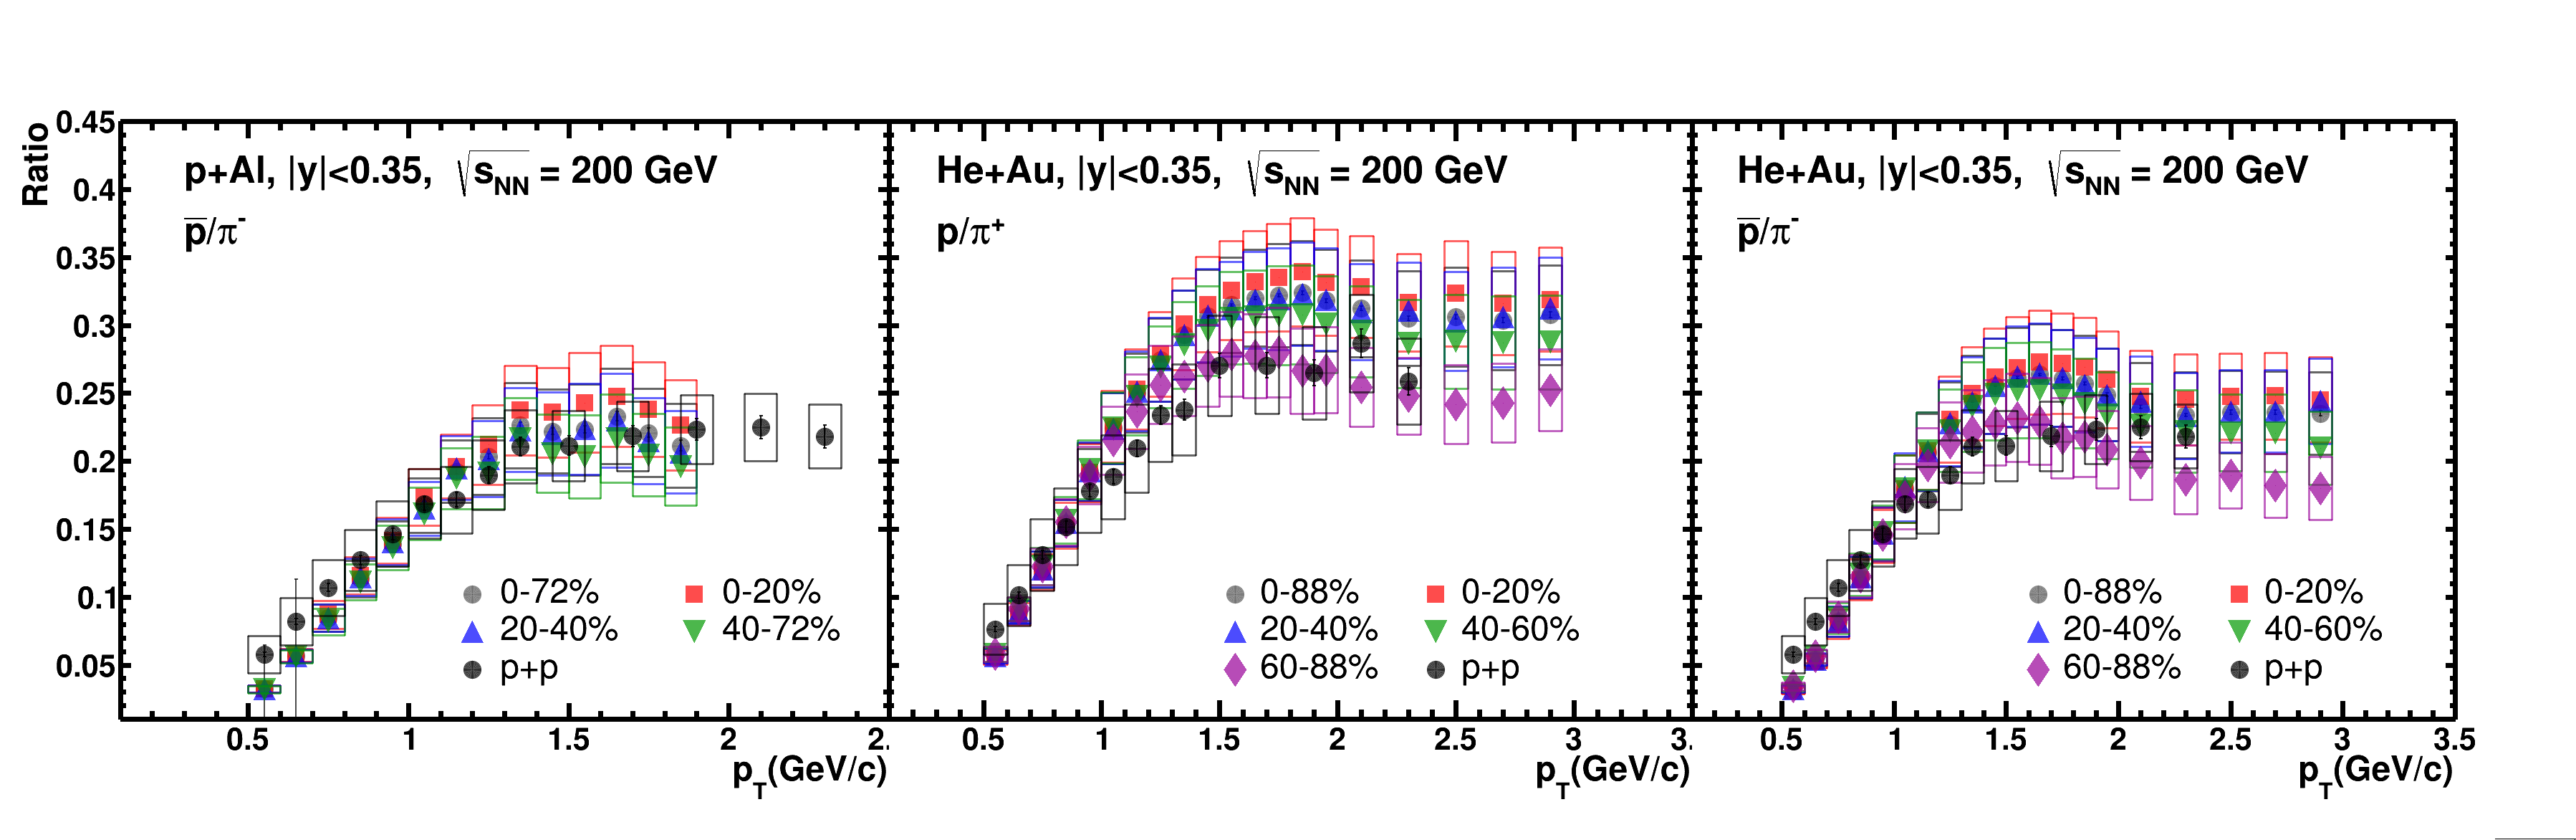
\includegraphics [width=1\linewidth]{Results/InOneCanvasHmy_small_p2pi}
	\caption{Значения отношений \ratppi, измеренные в различных центральностях $p$+Al и \heau \ столкновений.} 
	\label{img:Res_p2pi_small}
\end{figure}

На рисунке \ref{img:Res_p2pi_large} представлено сравнение отношений \prot/\pip \ и \aprot/\pim \ в различных центральностях Cu+Au и U+U систем столкновений.
Величины отношений $p$/$\pi$, измеренные в Cu+Au и U+U столкновениях, достигают значения 0,8, что в $\sim2$ раза превосходит максимальное значение $p$/$\pi$, измеренное в $p+p$ столкновениях. Также важно отметить, что значения \ratppi \ проявляют выраженную зависимость от центральности.
Увеличение значений \ratppi \ и их зависимость от центральности столкновения ранее были обнаружены в столкновениях Au+Au и интерпретированы в рамках рекомбинационной модели (см. Раздел \ref{ch1/Recombination}) \cite{Recombination1, Recombination2}.

Отношения \ratppi, измеренные в различных классах событий по центральности в легких системах столкновений (\pal \ и \heau) представлены на Рисунке \ref{img:Res_p2pi_small}. Зависимость отношений \ratppi \ от центральности, ярко выраженная в тяжелых системах столкновений, в столкновениях \pal \ не наблюдается. В столкновениях \heau \ отношения \ratppi \ проявляют слабую зависимость от центральности, которая однако незначима в связи с большими систематическими неопределенностями. 

\begin{figure}[] 
	\centerfloat
	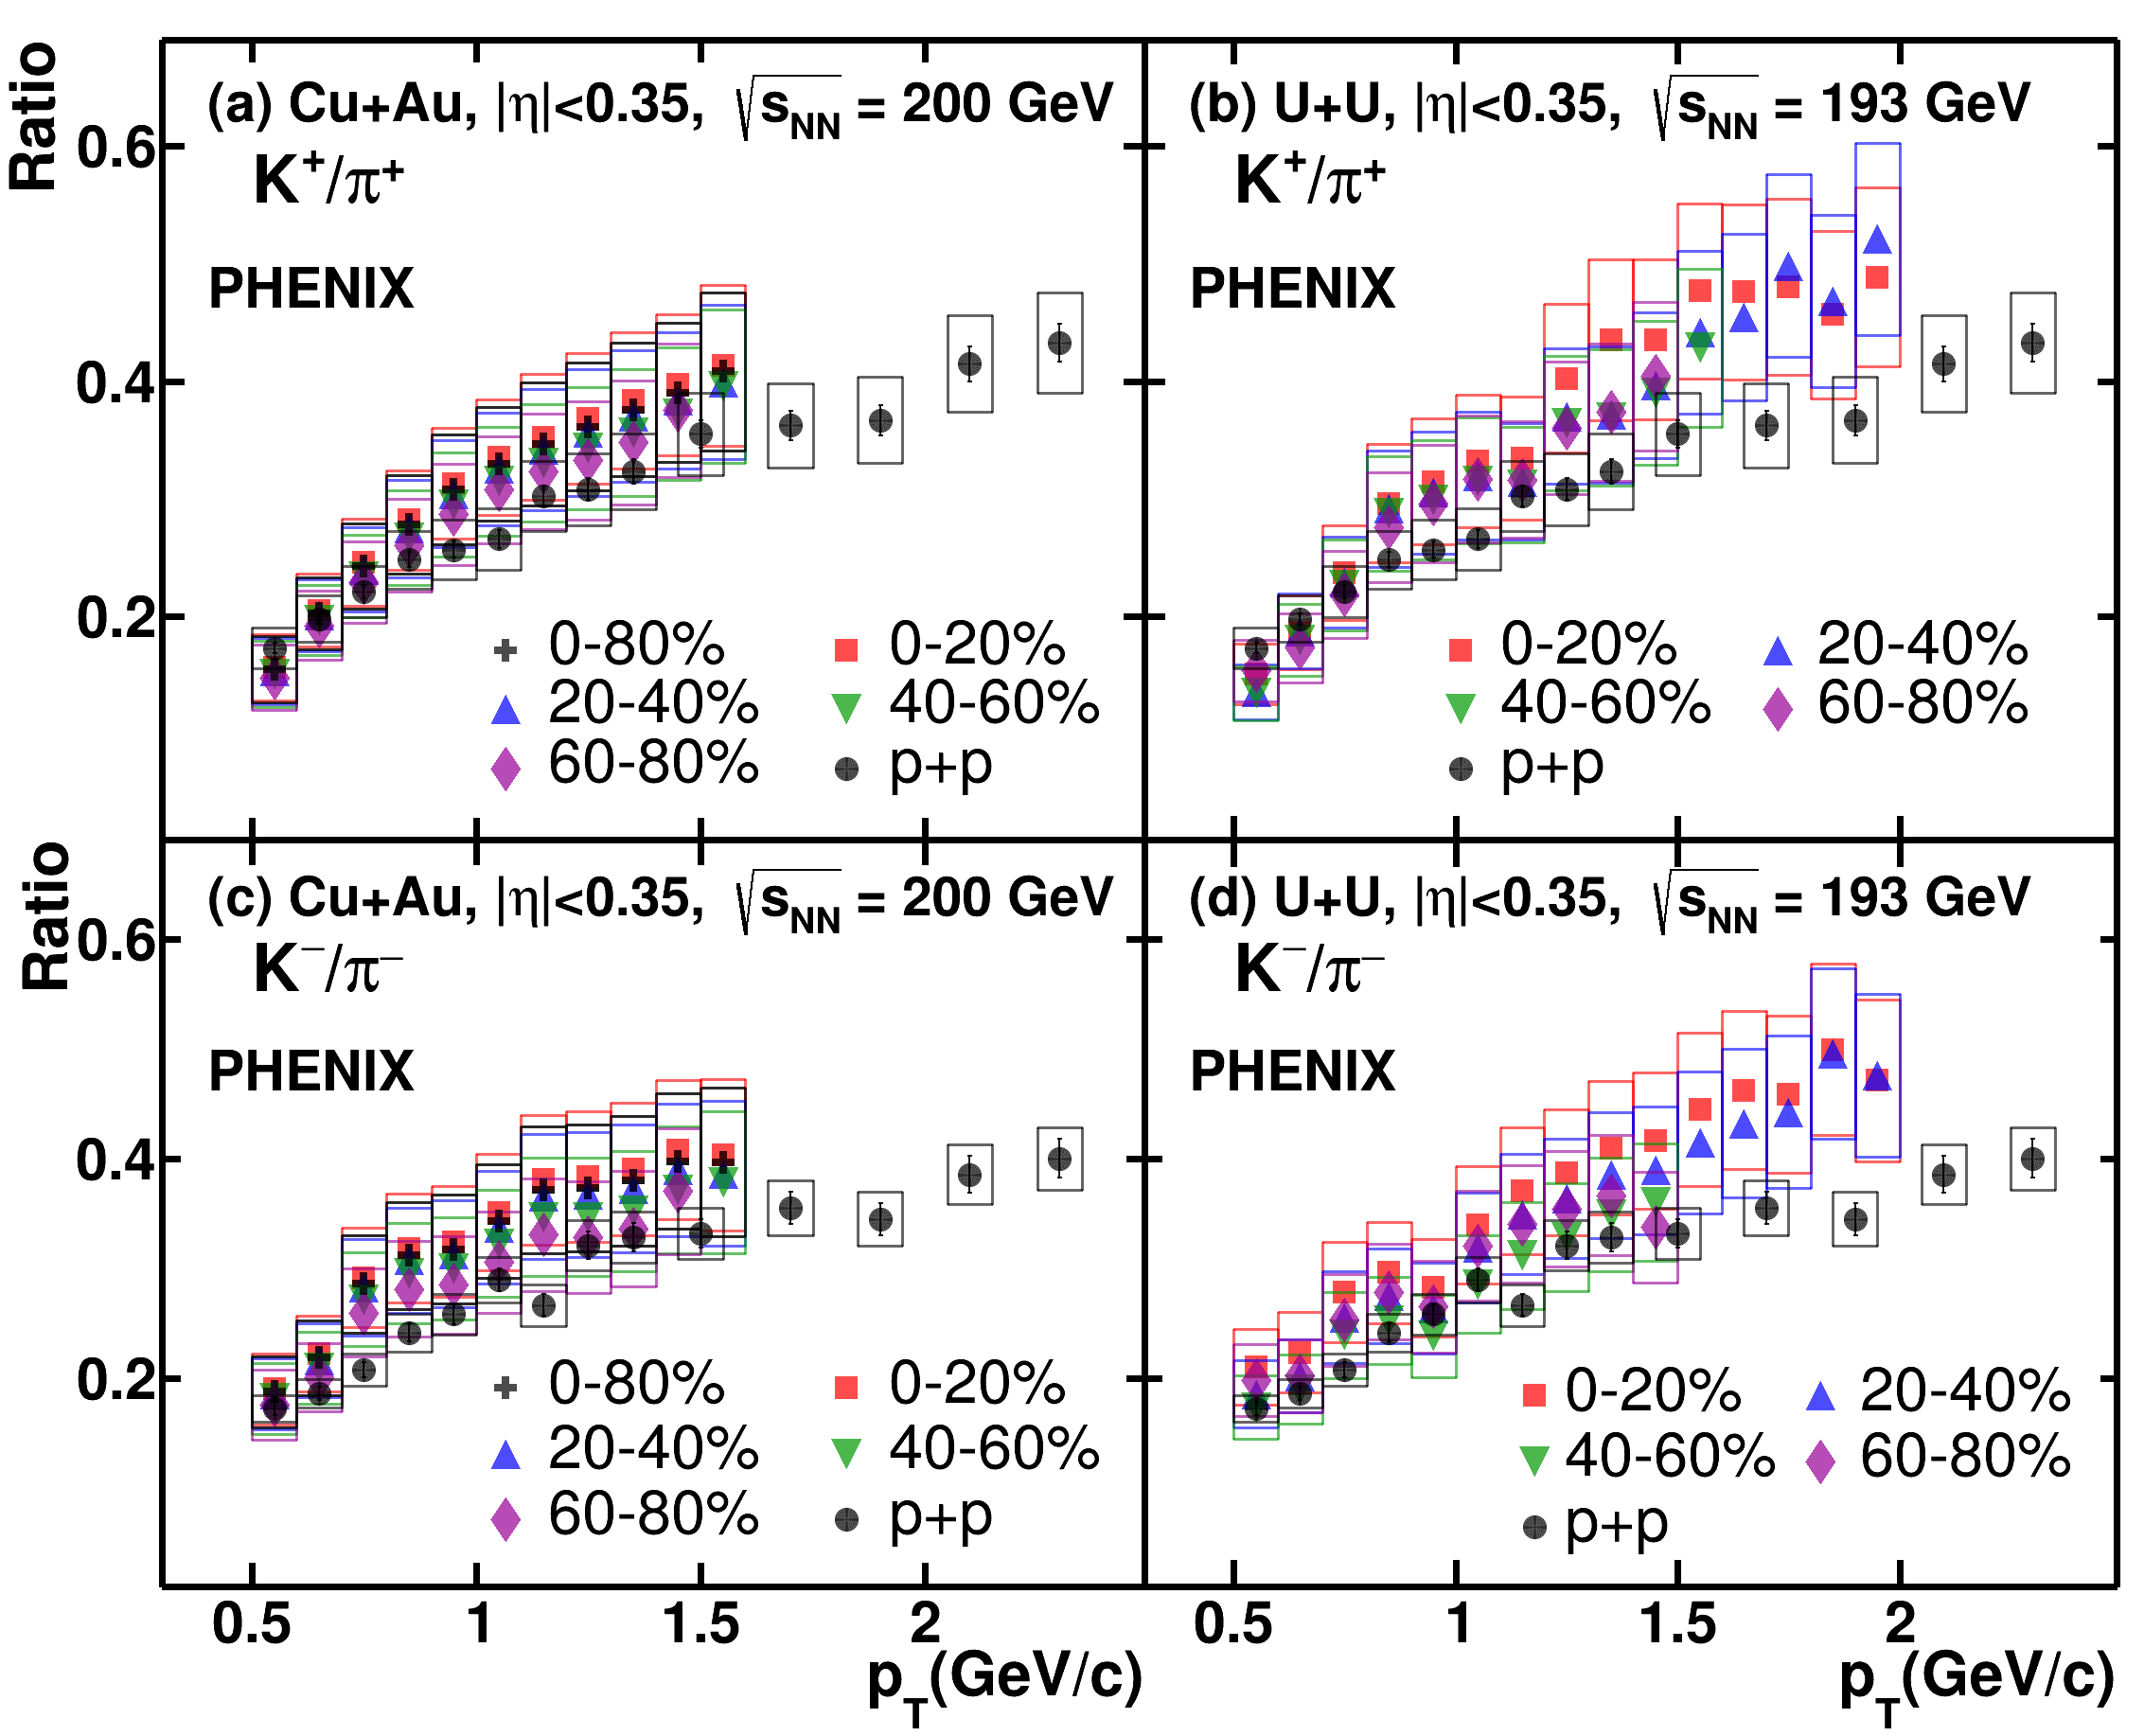
\includegraphics [width=0.65\linewidth]{Results/InOneCanvasHmy_large_K2pi}
	\caption{Значения отношений \ratKpi, измеренные в различных центральностях \cuau и \uu \ столкновений.} 
	\label{img:Res_K2pi_large}
\end{figure}

\begin{figure}[] 
	\centerfloat
	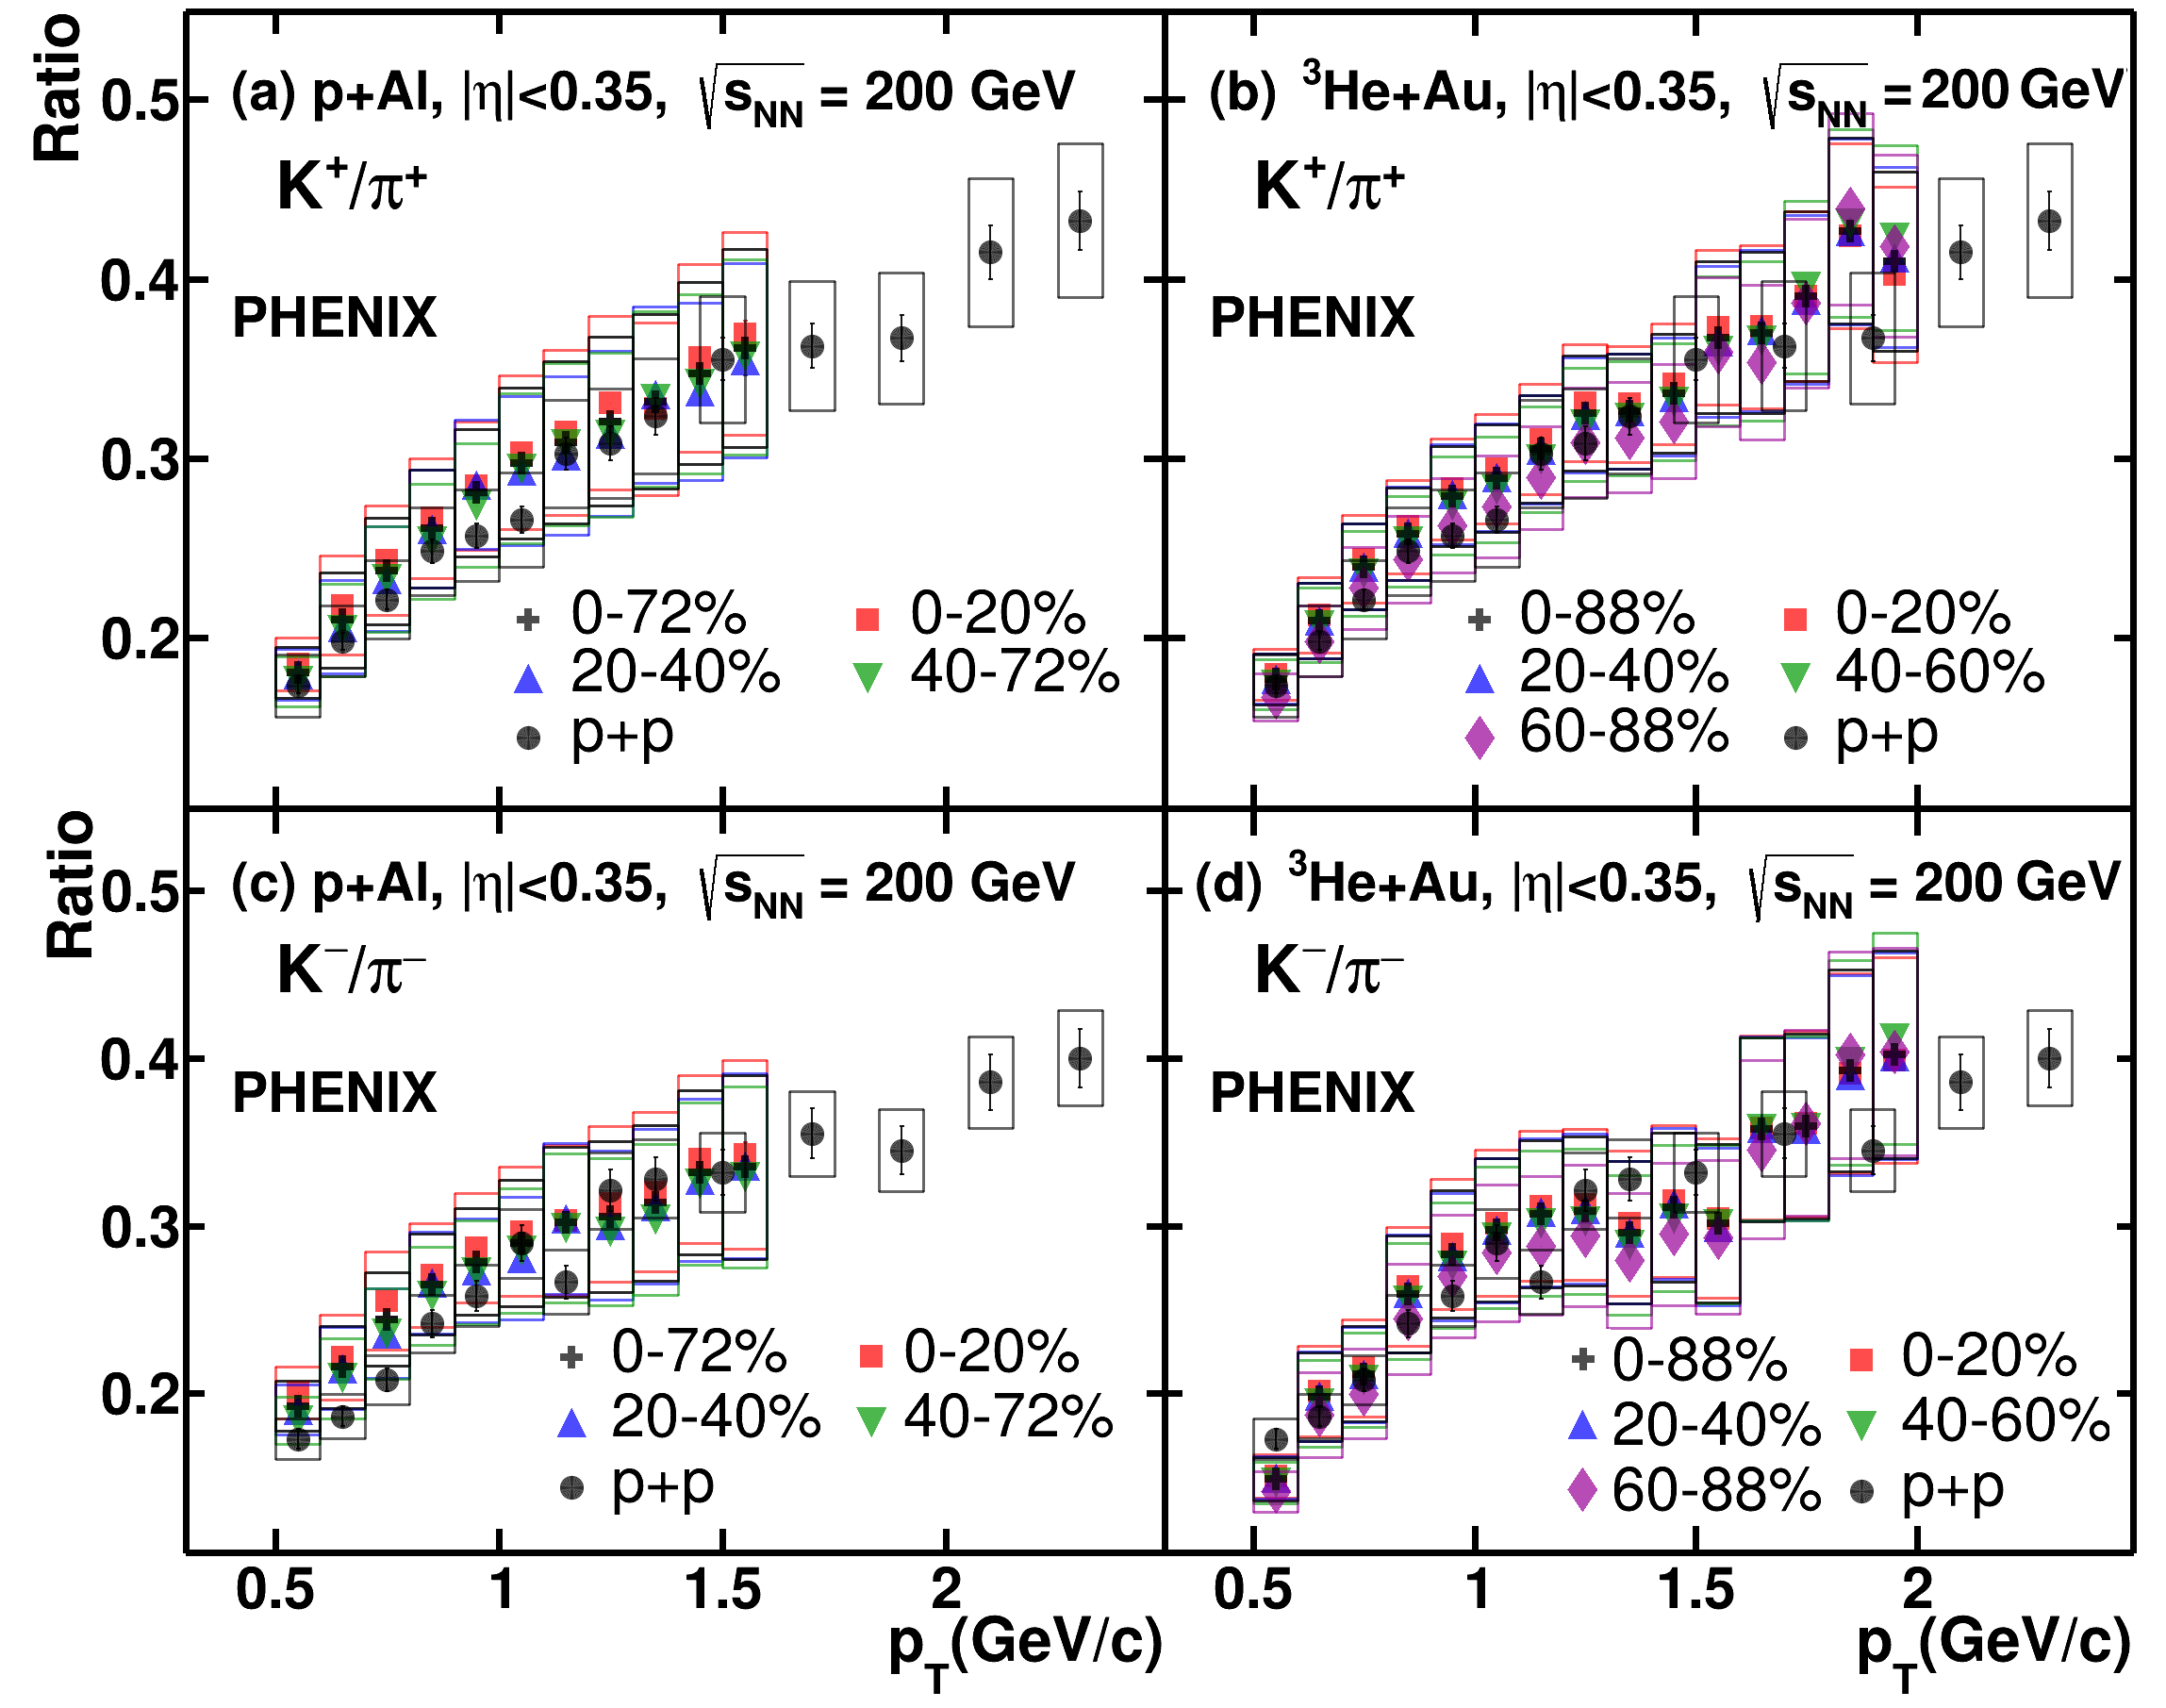
\includegraphics [width=0.65\linewidth]{Results/InOneCanvasHmy_small_K2pi}
	\caption{Значения отношений \ratKpi, измеренные в различных центральностях \pal и \heau столкновений.} 
	\label{img:Res_K2pi_small}
\end{figure}
Также были исследованы отношения инвариантных спектров, измеренные для двух типов мезонов: содержащего странный кварк $K$-мезона и $\pi$-мезона, состоящего только из $u$ и $d$ кварков, (\ratKpi).
Во всех рассматриваемых системах столкновений значения отношений \ratKpi \ проявляют слабую зависимость от центральности и по величине совпадают с результатами, полученными в $p+p$ столкновениях  (Рисунки \ref{img:Res_K2pi_large}, \ref{img:Res_K2pi_small}). 
%Намек на зависимость величин $k/\pi$ от центральности, наблюдаемый в тяжелых системах столкновений является проявлением эффекта увеличенного выхода странности.
           % Глава 4
\chapter{Интерпретация полученных результатов} \label{chapt5}

\section{Инвариантные спектры по поперечному импульсу} \label{sect5_spectra}

Форма инвариантных \pt-спектров, измеренных для заряженных адронов (Рисунки \ref{img:SpectraPt0}, \ref{img:SpectraPt1}) зависит от типа частиц.
% В логарифмическом масштабе инвариантные \pt-спектры, измеренные для \pipm-мезонов, вогнуты внутрь, инвариантные \pt-спектры, измеренные для \Kpm-мезонов, имеют форму прямой, а инвариантные \pt-спектры, измеренные для \prot \ и \aprot, выпуклы вверх.
Данное различие в формах инвариантных \pt-спектров заряженных адронов может быть количественно описано путем перехода к инвариантным спектрам по поперечной массе \mt, где $m_T = \sqrt{m_{0}^{2} + p_{T}^{2}}$, $m_0$ - масса адрона. 

В диапазоне поперечных масс $m_T-m_0$~$<$~1,5~ГэВ инвариантные \mt-спектры могут быть описаны в рамках модели гидродинамики \cite{PPG026, HydroPartonicCascade} и аппроксимированны экспоненциальной функцией \cite{ToutModels}:

\begin{equation}
	\label{eq:spectra_mt}
	\frac{1}{2\pi m_T} \frac{d^2 N}{dm_T dy}=\frac{1}{2\pi T (T+m_0)}\cdot A \cdot exp \left( -\frac{m_T - m_0}{T}\right)
\end{equation}
где $T$ -- параметр обратного наклона спектра;

$A$ -- нормировочный коэффициент, содержащий информацию о множественности рождения частиц в данном диа­пазон быстрот $dN/dy$.
%Модели гидродинамики описывают спектры заряженных адронов в центральных столкновениях в диапазоне \pt~$<$~1,5~ГэВ/с. Однако, эти модели оказываются несостоятельными при описании периферических столкновений и при описании спектров в области \pt~$>$~2~ГэВ/с. 

Инвариантные спектры по поперечной массе, измеренные для положительно и отрицательно заряженных адронов в различных центральностях \pal, \heau, Cu+Au и U+U столкновений представлены на Рисунках \ref{img:SpectraMt0}, \ref{img:SpectraMt1}. Аппроксимация спектров с помощью формулы \ref{eq:spectra_mt} изображена на Рисунках \ref{img:SpectraMt0}, \ref{img:SpectraMt1} черными прямыми линиями.

\begin{figure}[] 
	\centerfloat
	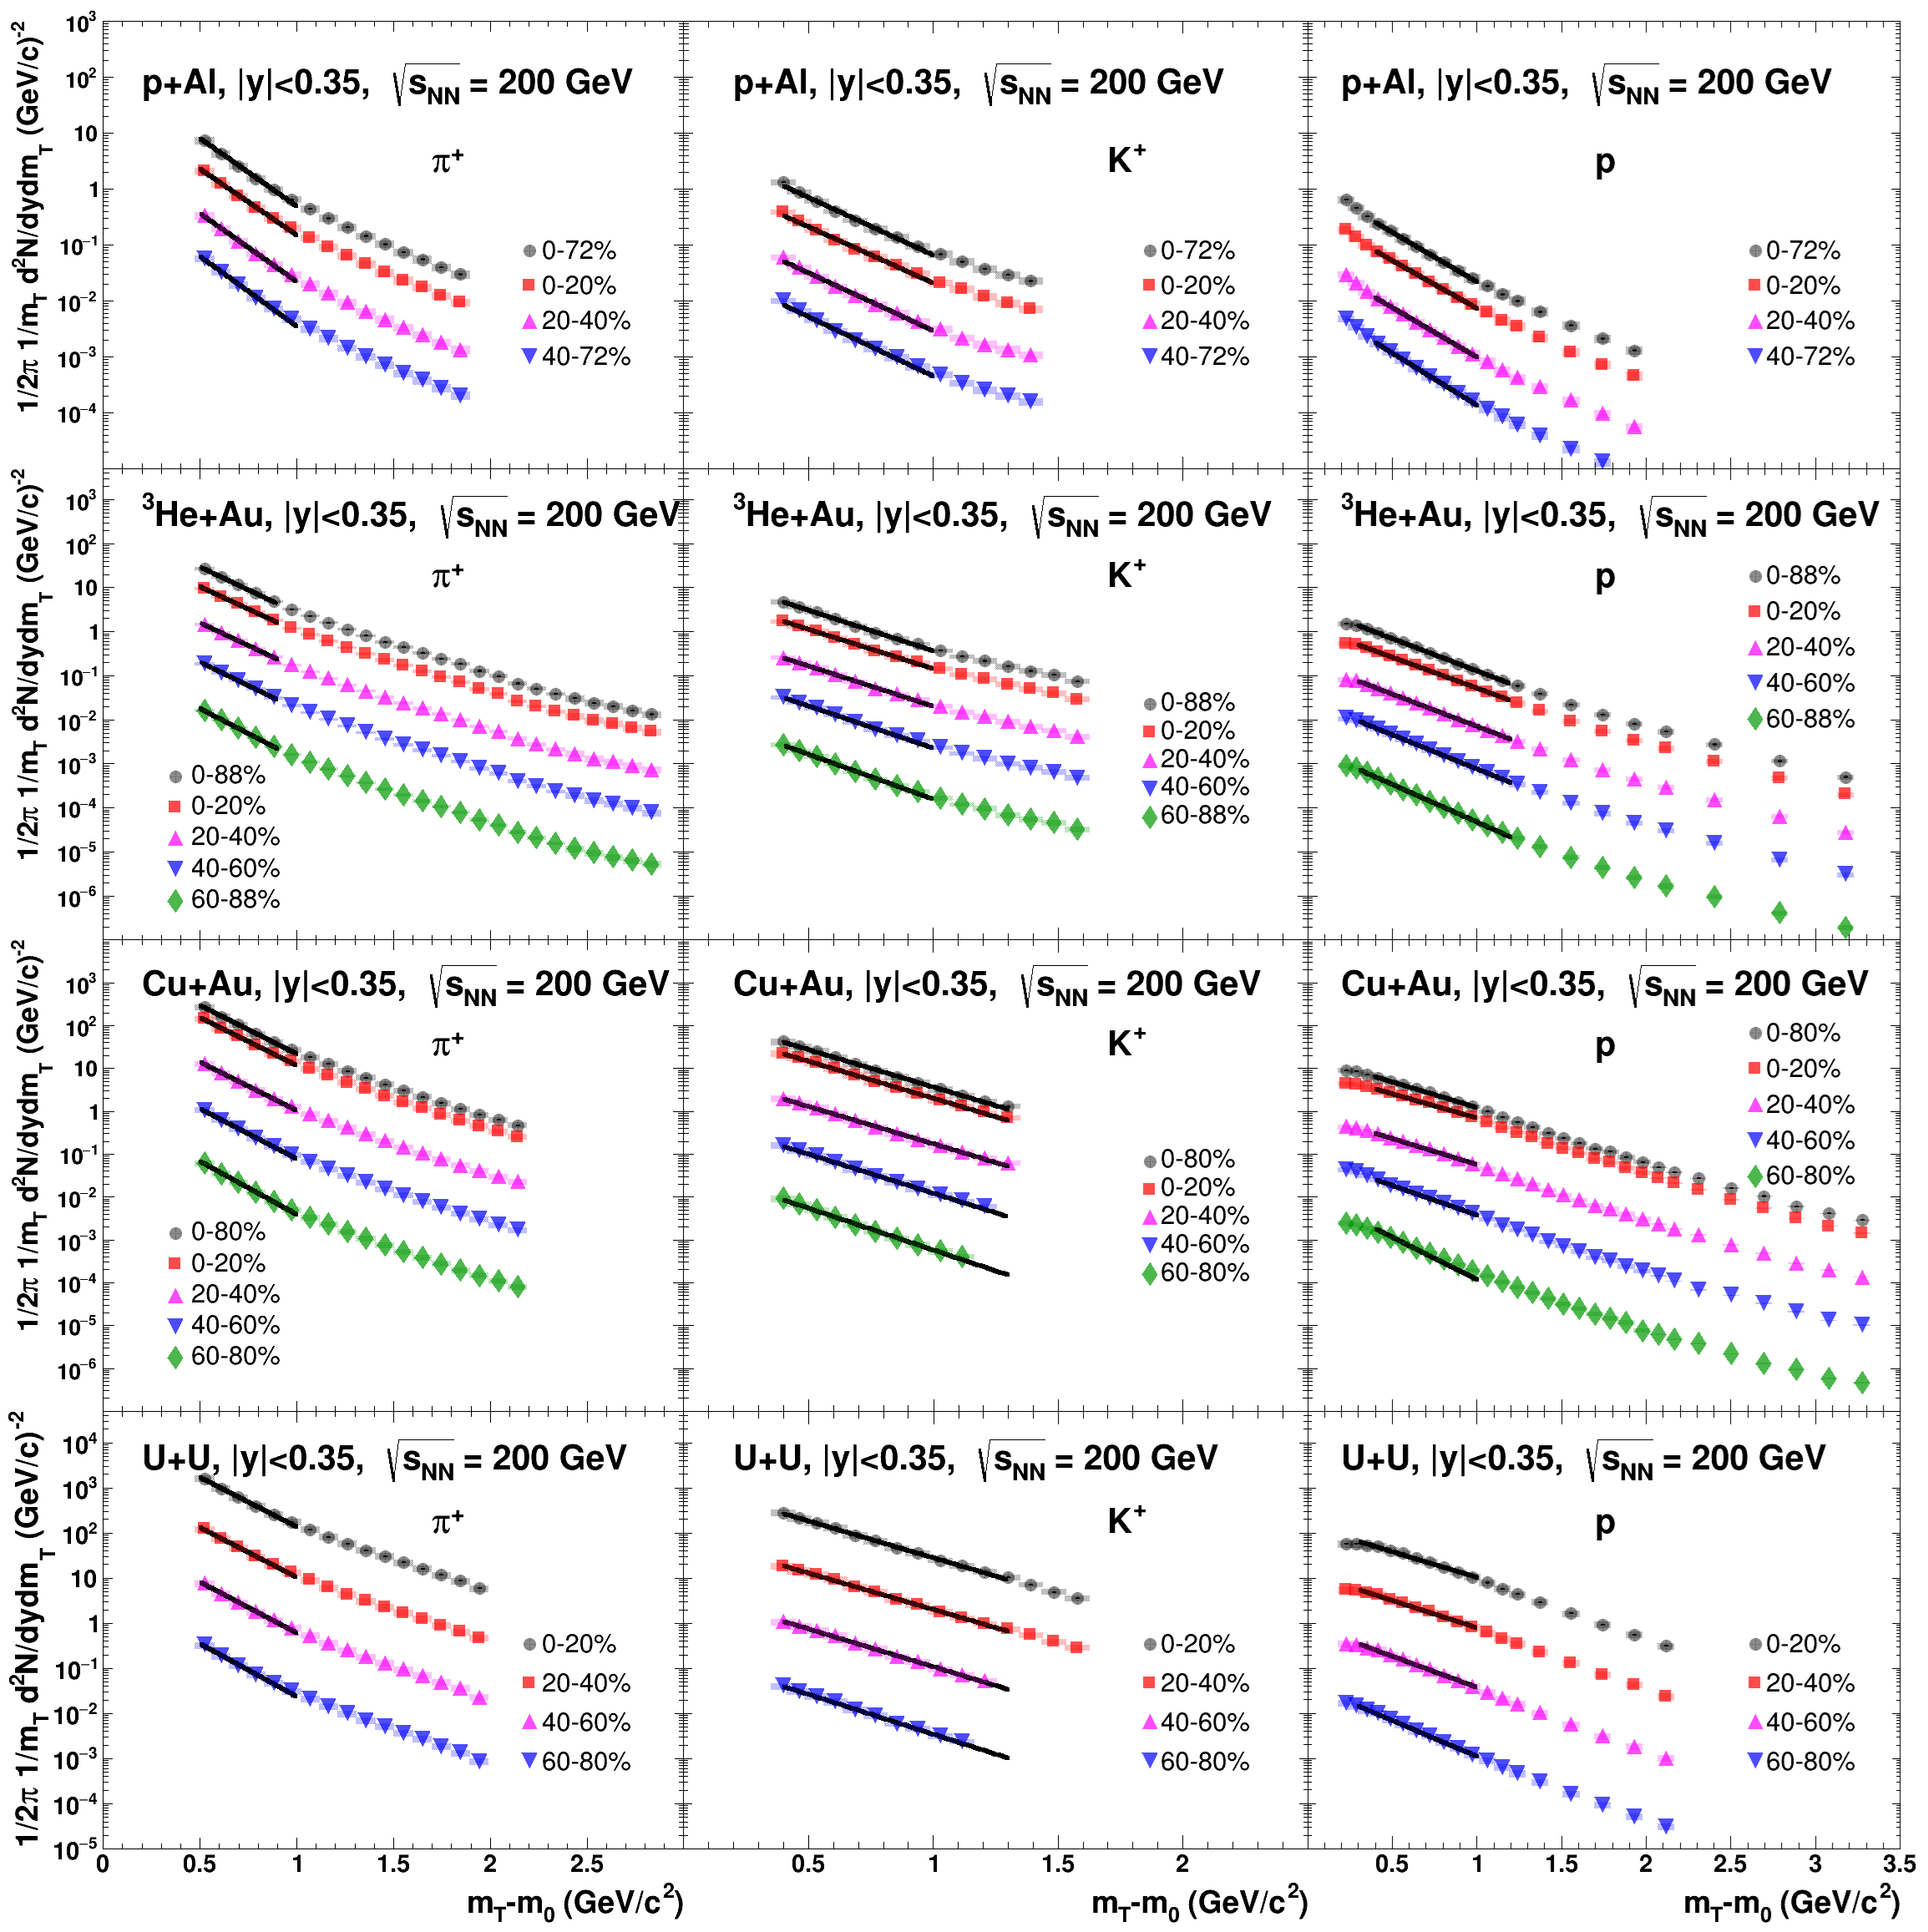
\includegraphics [width=1\linewidth]{Results/spectraDiss_mt_0.png}
	\caption{Инвариантные спектры по поперечному массе, измеренные для $\pi^+$, $K^+$, $p$ в различных центральностях \pal, \heau, Cu+Au и U+U столкновениях.} 
	\label{img:SpectraMt0}
\end{figure}
\begin{figure}[] 
	\centerfloat
	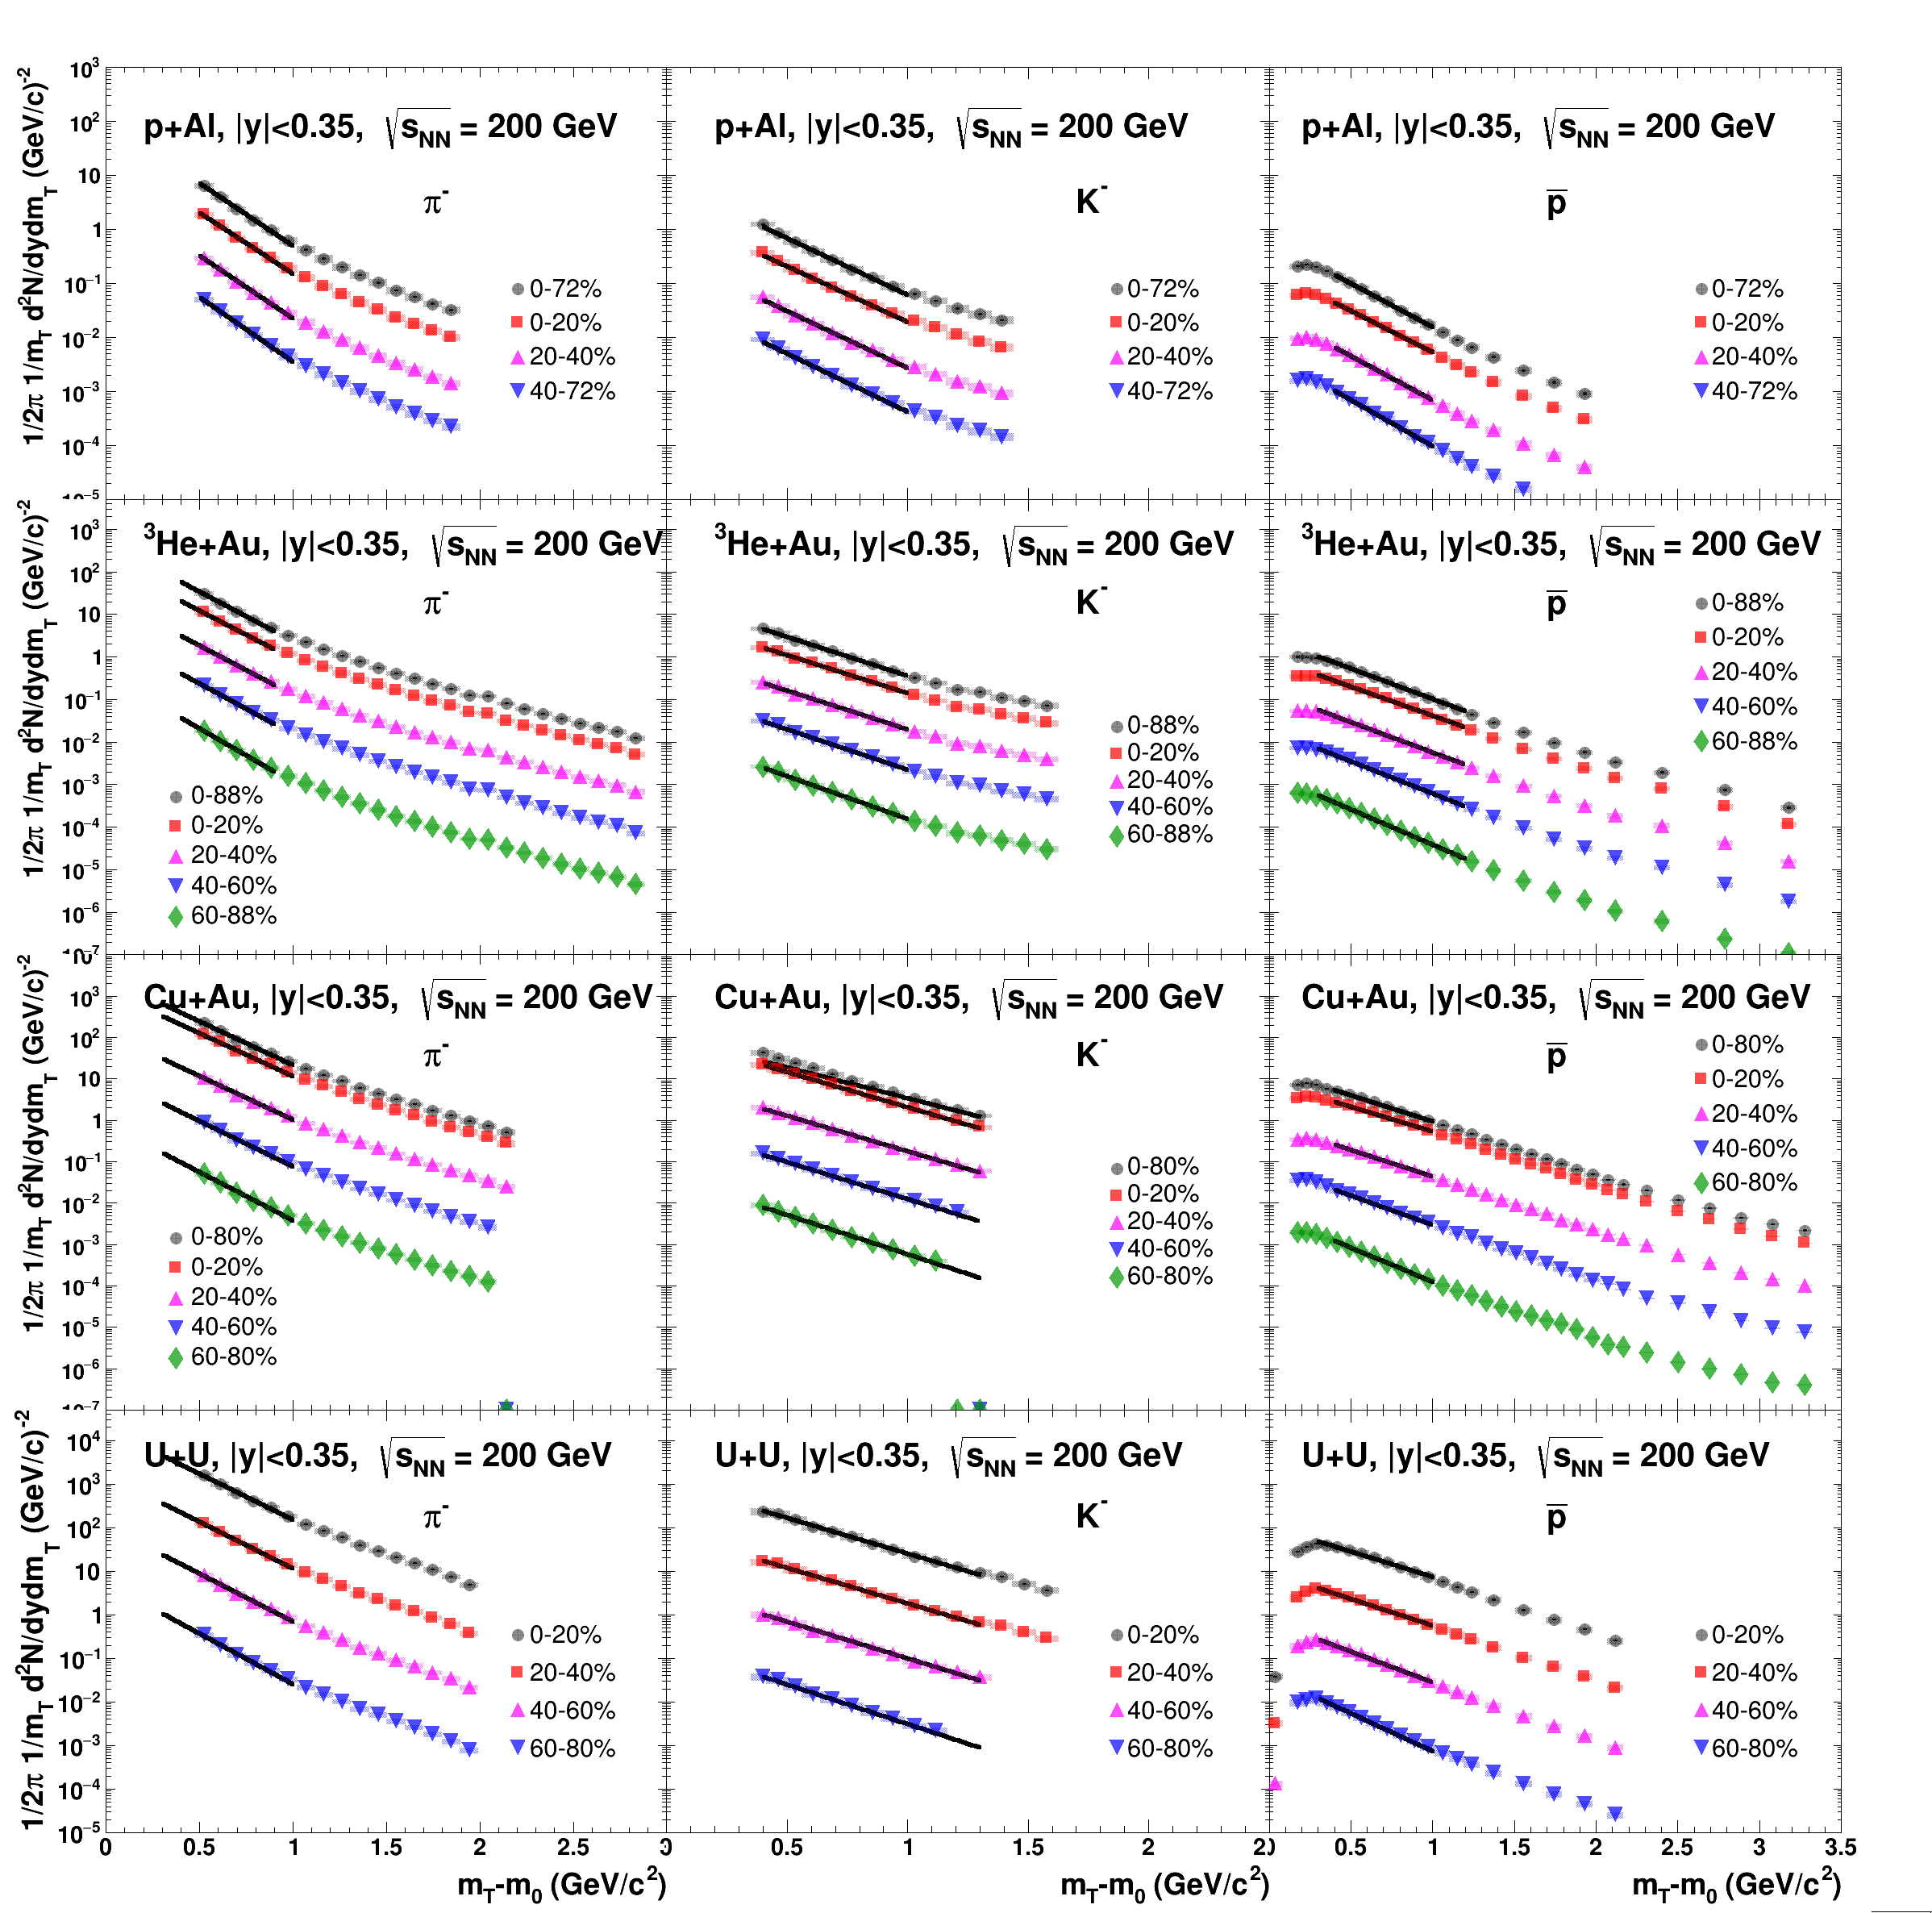
\includegraphics [width=1\linewidth]{Results/spectraDiss_mt_1.png}
	\caption{Инвариантные спектры по поперечному массе, измеренные для $\pi^-$, $K^-$, $\bar{p}$ в различных центральностях \pal, \heau, Cu+Au и U+U столкновениях.} 
	\label{img:SpectraMt1}
\end{figure}

Полученные параметры обратного наклона аппроксимационных прямых ($T$) приведены в Таблицах \ref{table:Tinv_pos}, \ref{table:Tinv_neg} и представлены на Рисунках \ref{img:Tinv0}, \ref{img:Tinv1} в зависимости от массы ($m_0$) положительно и отрицательно заряженных адронов в различных интервалах центральности столкновений \pal, \heau, Cu+Au, U+U. 
%Значения параметров $T$ увеличиваются с увеличением массы частиц во всех рассматриваемых инервалах центральности всех рассматриваемых систем столкновений.  

\begin{comment}
\begin{table}[]
	\caption{Значения параметров обратного наклона $T$ (ГэВ/$c^2$), вычисленные для положительно заряженных идентифицируемых адронов (\pip, \Kp, \prot) в столкновениях \pal, \heau, Cu+Au и U+U.}
	\label{table:Tinv_pos}
	
	\begin{tabularx}{\linewidth}
		{
			| >{\centering\arraybackslash}X
			| >{\centering\arraybackslash}X
			| >{\centering\arraybackslash}X
			| >{\centering\arraybackslash}X | }
		\hline
		\Npart     &  \pip & \Kp &\prot   \\ \hline
		\bfseries{\pal}      &     &     &      \\
		3,1 $\pm$ 0,1 &  178,88 $\pm$ 0,35  &  210,69 $\pm$ 0,77   &  --  \\
		4,4 $\pm$ 0,3 &  183,83 $\pm$ 0,28  &  216,10 $\pm$ 1,22   &  -- \\
		3,3 $\pm$ 0,1 &  178,20 $\pm$ 0,32  &  210,05 $\pm$ 1,43   &  --  \\
		1,6 $\pm$ 0,2 &  173,88 $\pm$ 0,46  &  204,74 $\pm$ 1,16   &  --  \\
		\hline
		\bfseries{\heau}       &     &     &      \\
		11,3 $\pm$ 0,5  &  208,70 $\pm$ 0,07  &  235,84 $\pm$ 0,24  & 295,74 $\pm$ 0,20   \\
		21,1 $\pm$ 1,3  &  214,33 $\pm$ 0,11  &  242,57 $\pm$ 0,38  & 309,27 $\pm$ 0,33    \\
		15,4 $\pm$ 0,9  &  209,84 $\pm$ 0,13  &  237,27 $\pm$ 0,44  & 296,44 $\pm$ 0,37  \\
		9,5 $\pm$ 0,6   &  202,71 $\pm$ 0,15  &  227,37 $\pm$ 0,53  & 280,01 $\pm$ 0,44    \\
		4,8 $\pm$ 0,3   &  191,01 $\pm$ 0,18  &  213,44 $\pm$ 0,66  & 254,22 $\pm$ 0,55    \\
		\hline
		\bfseries{Cu+Au}       &     &     &       \\
		70,4 $\pm$ 3,0  &  191,72 $\pm$ 0,01 &  249,33 $\pm$ 0,03 &  363,65 $\pm$ 0,09     \\
		154,8 $\pm$ 4,1 &  194,29 $\pm$ 0,12 &  251,43 $\pm$ 0,04 &  383,85 $\pm$ 0,13     \\
		80,4 $\pm$ 3,3  &  192,07 $\pm$ 0,02 &  249,14 $\pm$ 0,06 &  357,54 $\pm$ 0,16     \\
		34,9 $\pm$ 1,8  &  185,32 $\pm$ 0,03 &  238,05 $\pm$ 0,09 &  313,90 $\pm$ 0,20     \\
		11,5 $\pm$ 1,8  &  175,24 $\pm$ 0,05 &  222,76 $\pm$ 0,18 &  270,86 $\pm$ 0,28     \\
		\hline
		\bfseries{U+U}       &     &     &     \\
		330 $\pm$ 6 &  198,18 $\pm$ 0,02  &  266,49 $\pm$ 0,08  & 382,54 $\pm$ 0,19  \\
		259 $\pm$ 7 &  197,28 $\pm$ 0,04  &  269,42 $\pm$ 0,12  & 358,24 $\pm$ 0,23  \\
		65 $\pm$ 6  &  192,42 $\pm$ 0,06  &  259,69 $\pm$ 0,22  & 314,92 $\pm$ 0,32  \\
		\hline
		
	\end{tabularx}
\end{table}

\begin{table}[]
	\caption{Значения параметров обратного наклона $T$ (ГэВ/$c^2$), вычисленные для отрицательно заряженных идентифицируемых адронов (\pim, \Km, \aprot) в столкновениях \pal, \heau, Cu+Au и U+U.}
	\label{table:Tinv_neg}
	
	\begin{tabularx}{\linewidth}
		{
			| >{\centering\arraybackslash}X
			| >{\centering\arraybackslash}X
			| >{\centering\arraybackslash}X
			| >{\centering\arraybackslash}X | }
		\hline
		
		\Npart     & \pim & \Km & \aprot     \\ \hline
		\bfseries{\pal}      &     &     &     \\
		3,1 $\pm$ 0,1 &  187,36 $\pm$ 0,18  &  206,61 $\pm$ 0,78    &  269,51 $\pm$ 1,25    \\
		4,4 $\pm$ 0,3 &  192,56 $\pm$ 0,29  &  211,25 $\pm$ 1,21 &  275,14 $\pm$ 1,16    \\
		3,3 $\pm$ 0,1 &  186,96 $\pm$ 0,33  &  206,25 $\pm$ 1,46  &  266,62 $\pm$ 2,28    \\
		1,6 $\pm$ 0,2 &  181,99 $\pm$ 0,26  &  201,47 $\pm$ 1,18  &  254,20 $\pm$ 1,82    \\
		\hline
		\bfseries{\heau}       &     &     &      \\
		11,3 $\pm$ 0,5  &  187,25 $\pm$ 0,06  &  236,98 $\pm$ 0,25 &  303,59 $\pm$ 0,24    \\
		21,1 $\pm$ 1,3  &  191,58 $\pm$ 0,09  &  242,91 $\pm$ 0,39  &  317,40 $\pm$ 0,76    \\
		15,4 $\pm$ 0,9  &  188,33 $\pm$ 0,10  &  238,49 $\pm$ 0,46  &295,10 $\pm$ 0,18    \\
		9,5 $\pm$ 0,6   &  182,66 $\pm$ 0,13  &  229,34 $\pm$ 0,55  &  287,12 $\pm$ 0,54    \\
		4,8 $\pm$ 0,3   &  172,40 $\pm$ 0,15  &  215,99 $\pm$ 0,70  &  261,83 $\pm$ 0,66    \\
		\hline
		\bfseries{Cu+Au}       &     &     &         \\
		70,4 $\pm$ 3,0  &  205,41 $\pm$ 0,01  &  253,80 $\pm$ 0,03  & 344,75 $\pm$ 0,08    \\
		154,8 $\pm$ 4,1 &  208,57 $\pm$ 0,01  &  255,85 $\pm$ 0,09  & 365,18 $\pm$ 0,13    \\
		80,4 $\pm$ 3,3  &  205,67 $\pm$ 0,02  &  253,34 $\pm$ 0,05  & 338,92 $\pm$ 0,15    \\
		34,9 $\pm$ 1,8  &  197,72 $\pm$ 0,03  &  243,35 $\pm$ 0,09  & 306,48 $\pm$ 0,20    \\
		11,5 $\pm$ 1,8  &  186,06 $\pm$ 0,05  &  228,90 $\pm$ 0,18  & 263,38 $\pm$ 0,29    \\
		\hline
		\bfseries{U+U}       &     &     &       \\
		330 $\pm$ 6 &  205,84 $\pm$ 0,21  &  265,80 $\pm$ 0,08  &  374,48 $\pm$ 0,21    \\
		259 $\pm$ 7 &  202,39 $\pm$ 0,03  &  266,36 $\pm$ 0,11  &  353,94 $\pm$ 0,26    \\
		65 $\pm$ 6  &  197,74 $\pm$ 0,06  &  257,80 $\pm$ 0,20  &  308,57 $\pm$ 0,35    \\
		\hline
	\end{tabularx}
\end{table}



\begin{table}[]
	\caption{Значения аппроксимационных параметров \To \ и \ut, вычисленные для различных систем столкновений: \pal, \heau, Cu+Au, U+U.}
	\label{table:To_ut}
	
	\begin{tabularx}{\linewidth}
		{
			| >{\centering\arraybackslash}X
			| >{\centering\arraybackslash}X
			| >{\centering\arraybackslash}X
			| >{\centering\arraybackslash}X
			| >{\centering\arraybackslash}X | }
		\hline
		
		\Npart     & $T_{0}^{+}$ & $T_{0}^{-}$  & $\left<u_{t}\right>^{+}$ & $\left<u_{t}\right>^{-}$   \\ \hline
		
		\bfseries{\pal}       &     &     &      &    \\
		3,1$\pm$0,1  &  167,9 $\pm$ 2,1  &  166,4 $\pm$ 15,2  &  0,2 $\pm$ 0,1  &  0,3 $\pm$ 0,1   \\
		4,4$\pm$0,3   &  171 $\pm$ 0,9  &  171,3 $\pm$ 15,9  &  0,2 $\pm$ 0,1  &  0,3 $\pm$ 0,1 \\
		3,3$\pm$0,1  &  167,9 $\pm$ 2,1  &  167,8 $\pm$ 14,3  &  0,2 $\pm$ 0,1  &  0,3 $\pm$ 0,1    \\
		1,6$\pm$0,2  &  164 $\pm$ 4,3  &  163,8 $\pm$ 11,2  &  0,2 $\pm$ 0,1  &  0,3 $\pm$ 0,1    \\
		\hline
		\bfseries{\heau}       &     &     &      &    \\
		11,3$\pm$0,5  &  188,9 $\pm$ 10,2  &  166,2 $\pm$ 1,7  &  0,3 $\pm$ 0,1  &  0,3 $\pm$ 0,1    \\
		21,1$\pm$1,3  &  193 $\pm$ 12,4  &  166,4 $\pm$ 3,2  &  0,3 $\pm$ 0,1  &  0,3 $\pm$ 0,1    \\
		15,4$\pm$0,9  &  188,9 $\pm$ 9,8  &  167,5 $\pm$ 1,2  &  0,3 $\pm$ 0,1  &  0,3 $\pm$ 0,1    \\
		9,5$\pm$0,6  &  185 $\pm$ 8,5  &  164,6 $\pm$ 0,2  &  0,3 $\pm$ 0,1  &  0,3 $\pm$ 0,1    \\
		4,8$\pm$0,3  &  177 $\pm$ 4,9  &  158,3 $\pm$ 3,4  &  0,2 $\pm$ 0,1  &  0,3 $\pm$ 0,1    \\
		\hline
		\bfseries{Cu+Au}       &     &     &      &    \\
		70,4$\pm$3,0 &  153,9 $\pm$ 16,6  &  176 $\pm$ 11,9  &  0,4 $\pm$ 0,1  &  0,4 $\pm$ 0,1 \\
		154,8$\pm$4,1  &  150 $\pm$ 23,9  &  172,8 $\pm$ 19,7  &  0,4 $\pm$ 0,1  &  0,4 $\pm$ 0,1    \\
		80,4$\pm$3,3  &  157 $\pm$ 14,5  &  178,1 $\pm$ 10,2  &  0,4 $\pm$ 0,1  &  0,4 $\pm$ 0,1    \\
		34,9$\pm$2,9  &  160,9 $\pm$ 3,8  &  177,7 $\pm$ 2,3  &  0,4 $\pm$ 0,1  &  0,3 $\pm$ 0,1    \\
		11,5$\pm$1,8 &  159,9 $\pm$ 4,5  &  175,8 $\pm$ 7,5  &  0,3 $\pm$ 0,1  &  0,3 $\pm$ 0,1    \\
		\hline
		\bfseries{U+U}       &     &     &      &    \\
		330$\pm$6 &  159,9 $\pm$ 12  &  170,8 $\pm$ 13,2  &  0,4 $\pm$ 0,1  &  0,4 $\pm$ 0,1  \\
		259$\pm$7 &  168,9 $\pm$ 0,6  &  174,7 $\pm$ 2,9  &  0,4 $\pm$ 0,1  &  0,4 $\pm$ 0,1    \\
		65$\pm$6   &  175,9 $\pm$ 11,4  &  182,6 $\pm$ 9,6  &  0,3 $\pm$ 0,1  &  0,3 $\pm$ 0,1 \\
		\hline
	\end{tabularx}
\end{table}
\end{comment}

В рамках модели термодинамического расширения зависимости \cite{Thermal1, Coalescence_models, ToutModels} $T$($m_0$) в свою очередь могут быть аппроксимированы (см. раздел \ref{sectRes_spectra}) линейной функцией с параметрами \To \ и \ut \cite{PPG026}:
\begin{equation}
	\label{eq:InvSlope}
	T = T_0 +m_0 \left< u_t\right>^2
\end{equation}
где параметр $T_0$ интерпретируется как температура при которой происходит кинетическое <<вымораживание>> (прекращение взаимодействия частиц), а \ut \ -- как поперечная скорость коллективного движения адронов. 
%Также параметр $T_0$ можно интерпретировать как линейную экстраполяцию параметра обратного наклона $T$ к нулевой массе $m=0$.
Линейная аппроксимация зависимости $T(m_0)$ с использованием уравнения. \ref{eq:InvSlope} изображена на Рисунках \ref{img:Tinv0}, \ref{img:Tinv1} пунктирными линиями.

\begin{figure}[] 
	\centerfloat
	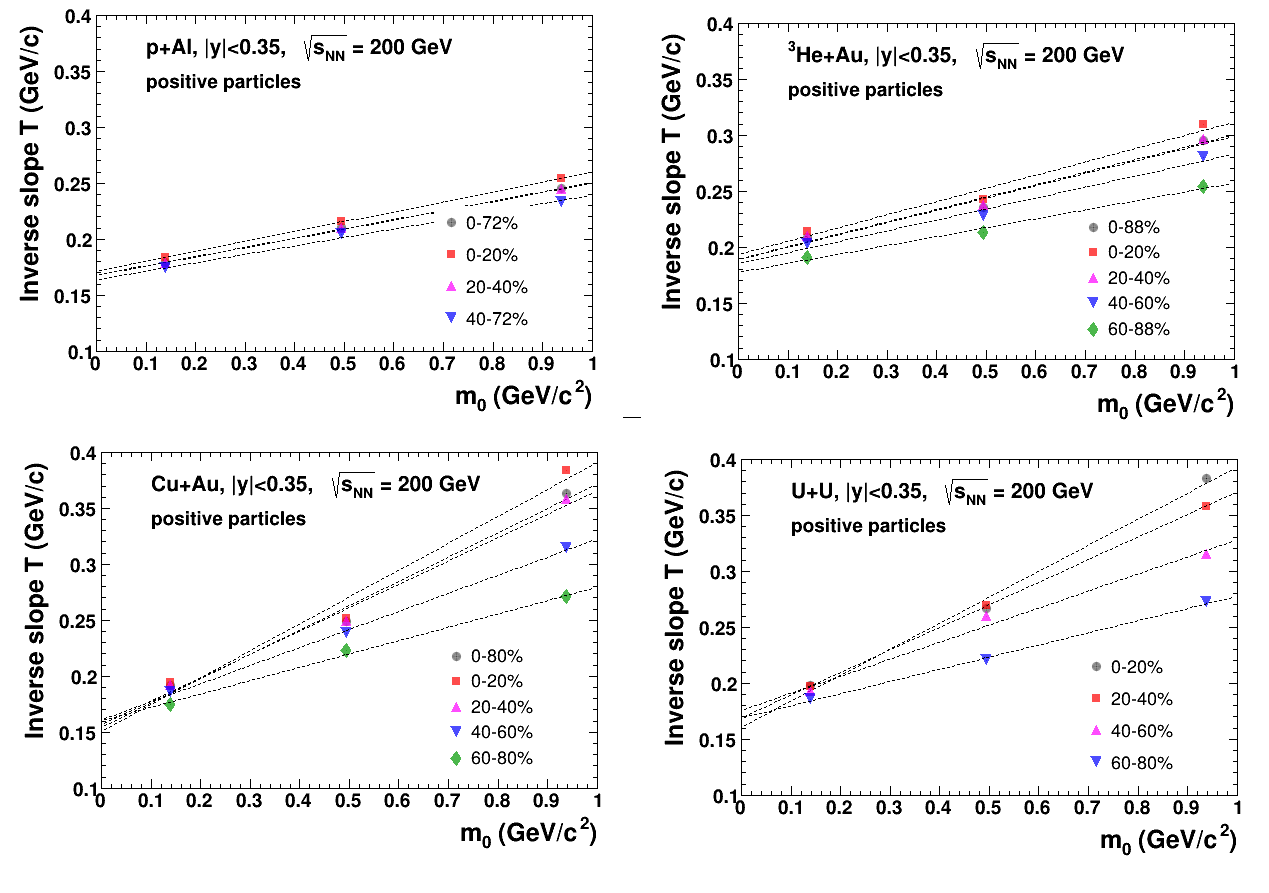
\includegraphics [width=0.85\linewidth]{Results/Tgr0.png}
	\caption{Зависимость величины параметра обратного наклона $T$ от массы \pip, \Kp, \prot \ в различных центральностях \pal, \heau, Cu+Au и U+U столкновениях.} 
	\label{img:Tinv0}
\end{figure}
\begin{figure}[] 
	\centerfloat
	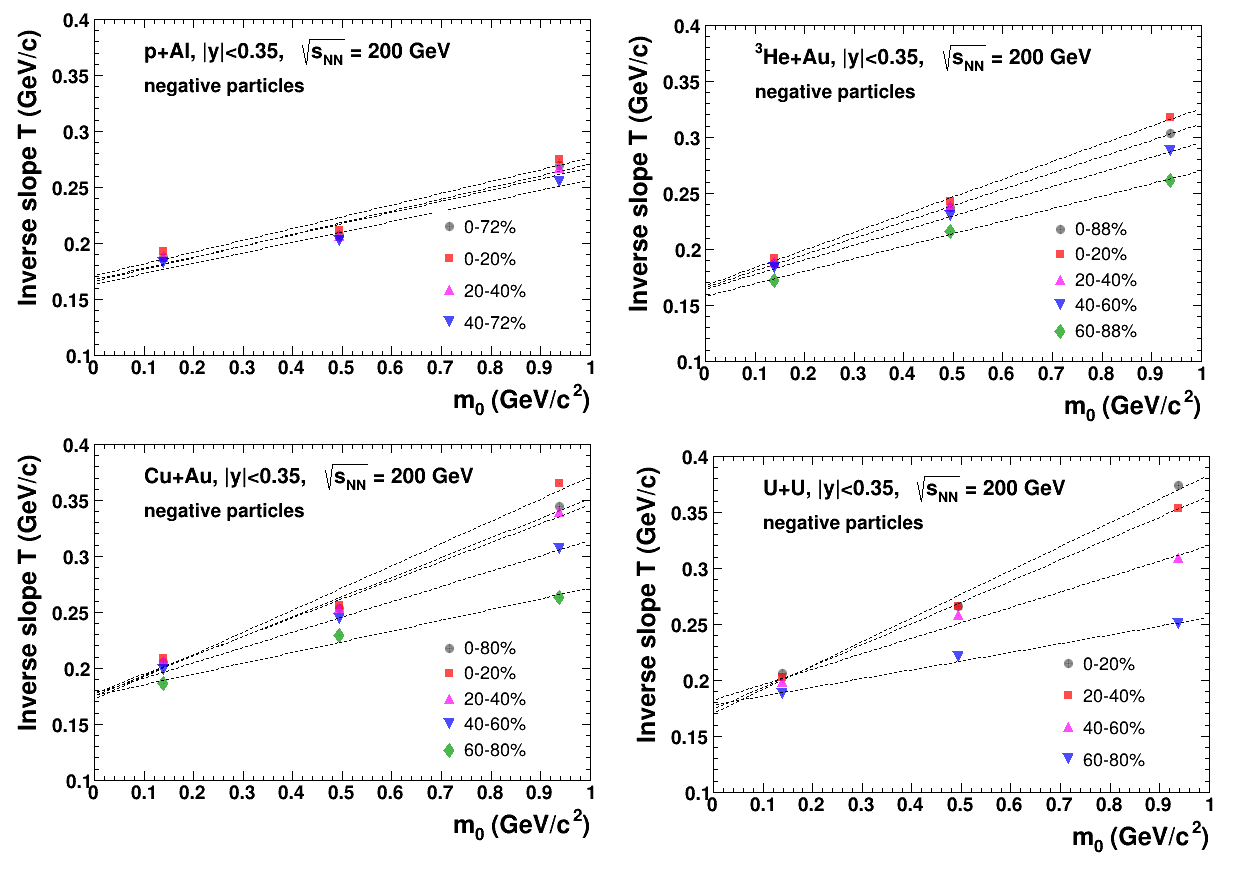
\includegraphics [width=0.85\linewidth]{Results/Tgr1.png}
	\caption{Зависимость величины параметра обратного наклона $T$ от массы \pim, \Km, \aprot \ в различных центральностях \pal, \heau, Cu+Au и U+U столкновениях.} 
	\label{img:Tinv1}
\end{figure}


\begin{figure}[ht]
	\centerfloat{
		\hfill
		\subcaptionbox{ }{
			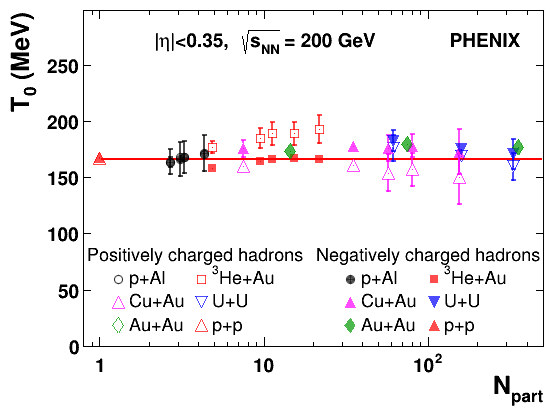
\includegraphics[width=0.45\linewidth]{Results/T0_Npart.png}
		}
		\hfill
		\subcaptionbox{ }{
			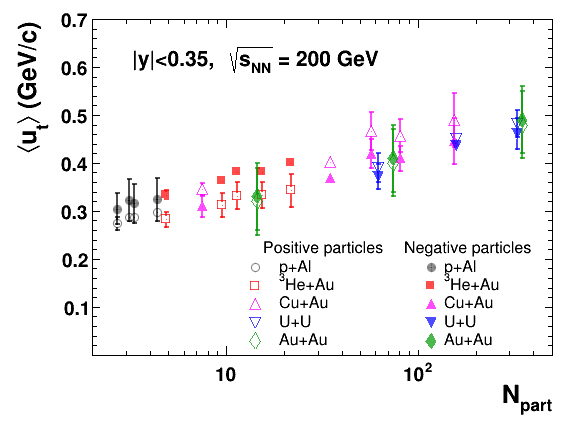
\includegraphics[width=0.45\linewidth]{Results/ut_Npart.png}}
		\hfill
	}
	\caption{Зависимость а) температуры вымораживания $T_0$ и  б) скорости поперечного потока $u_T$ от количество нуклонов участников \Npart.}
	\label{fig:TuNpart}
\end{figure}

Полученные значения $T_0$ и $\left< u_t \right>$ приведены в Таблице \ref{table:To_ut}, а также представлены на Рисунке \ref{fig:TuNpart} в зависимости от значений \Npart. Из приведенных Таблиц \ref{table:To_ut} и Рисунка \ref{fig:TuNpart} а) видно, что величины параметра $T_0$ не проявляют значимой зависимости от значений \Npart. 
Среднее значение $T_0$ равно $166,1 \pm 2,2$ МэВ и показано на Рисунке \ref{fig:TuNpart} а) сплошной красной линией.
Величины $\left< u_t \right>$ увеличиваются с ростом \Npart. Зависимость $\left< u_t \right>(\left< N_{part} \right>)$ была аппроксимирована с помощью логарифмической функции  $p_1 \cdot log(p_2 \cdot \left< N_{part} \right>)$, где $p_1 = 0,0345 \pm 0,0003$, $p_2 = 3196 \pm 342$. Данный результат находится в соответствии с гидродинамической картиной столкновения и моделью термодинамического расширения \cite{HydroPartonicCascade}.

\newpage
\section{Интегральные отношения выходов $p/\pi$} \label{sect5_integratedRatio}
\begin{figure}[] 
	\centerfloat
	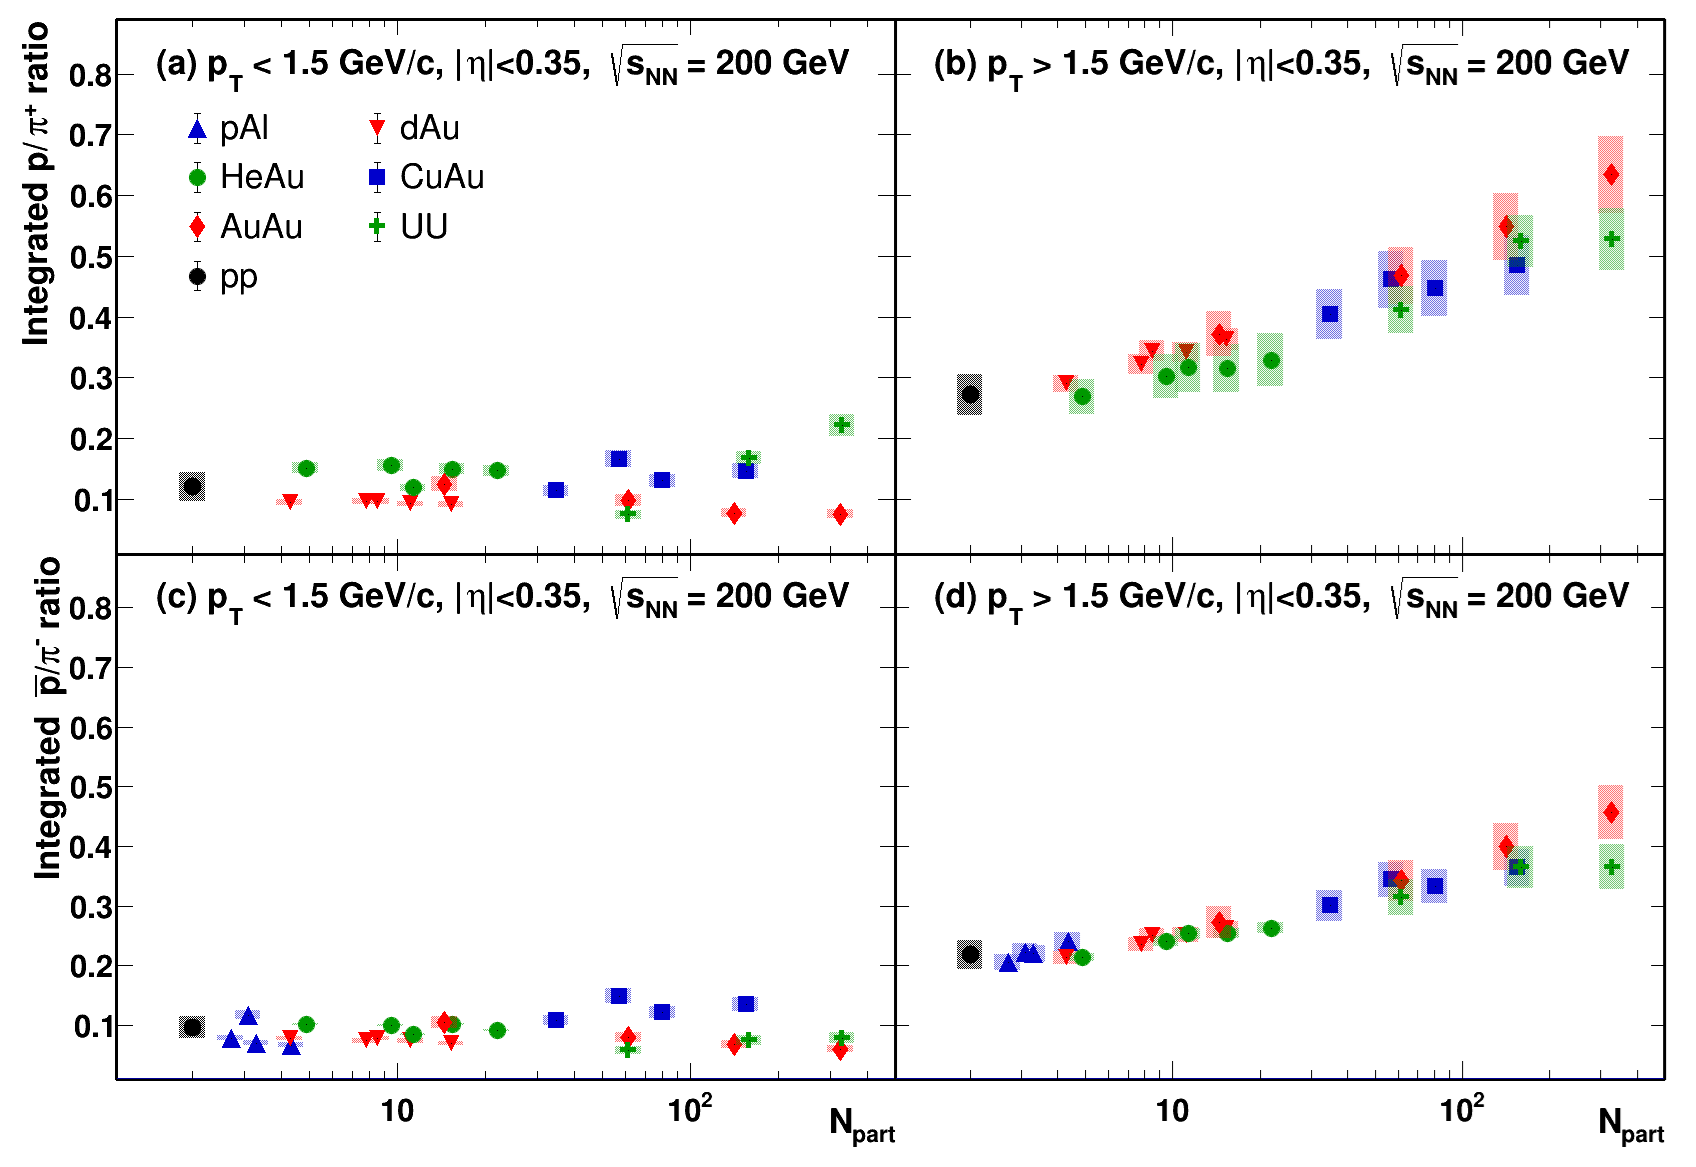
\includegraphics [width=0.85\linewidth]{Results/IntegratedRatio.png}
	\caption{Интегральные отношения $p/\pi^+$ и $\bar{p}/\pi^-$, измеренные как функции $\left< N_{part} \right>$ в области малых $p_T$ ($p_T < 1,5$ ГэВ/$c$) и средних $p_T$ ($p_T > 1,5$ ГэВ/$c$).} 
	\label{img:IntegratedRatio}
\end{figure}

На Рисунке \ref{sect5_integratedRatio} представлены интегральные отношения $p/\pi^+$ и $\bar{p}/\pi^-$ в области мылаых $p_T$ ($p_T < 1,5$ ГэВ/$c$) и средних $p_T$ ($p_T > 1,5$ ГэВ/$c$) как функции \Npart. Значения $p/\pi^+$ и $\bar{p}/\pi^-$, интегрированные в области малых $p_T$ (Рисунок \ref{sect5_integratedRatio} а), в)), не проявляют значимой зависимости от \Npart. Значения $p/\pi^+$ и $\bar{p}/\pi^-$, интегрированные в области средних $p_T$ (Рисунок \ref{sect5_integratedRatio} а), в)), возрастают с увеличением \Npart. Поскольку отношение $\bar{p}/p$ приблизительно равно 0,73 \cite{PPG026} при всех значениях \Npart, значения интегральных отношений  $p/\pi^+$ превышают значения интегрировальных отношений $\bar{p}/\pi^-$.

Согласно модели рекомбинации, импульс образующегося адрона складывается их импульсов составляющих его кварков. Поэтому барионные инвариантные $p_T$ спектры оказываются сдвинутыми относительно мезонных инвариантных $p_T$ спектров в сторону больших $p_T$, что приводит к увеличению образования барионов по сравнению с образованием мезонов в области средних $p_T$. Таким образом, полученные значения интегральных отношений $p/\pi^+$ и $\bar{p}/\pi^-$ подтверждают предположение о том, что влияние процессов рекомбинации возрастает с увеличением значений \Npart.

\newpage
\section{Сравнение с результатами моделирования} \label{sect5_models}

Для более глубокого анализа полученных экспериментальных данных, было осуществлено моделирование \pal, \heau, Cu+Au столкновений при $\sqrt{s_{NN}}$ = 200 ГэВ и U+U столкновений при $\sqrt{s_{NN}}$ = 193 ГэВ с помощью программных пакетов PYTHIA/ANGANTYR 8,3 \cite{pythia} и AMPTsm \cite{AMPT}.
Принципиальное различие данных программных пакетов состоит в различных моделях адронизации партонов: пакет PYTHIA8,3/ANGANTYR \cite{pythia} реализует модель адронизации Лунда \cite{FragmentationLund}, в то время как AMPT \cite{AMPT} в версии с плалением струн (AMPTsm) учитывает рекомбинационные процессы адронизации \cite{Recombination1, Recombination2}.

\begin{comment}
	\subsection{PYTHIA8}
	\label{subsect5_pythia}
	PYTHIA 8,3 - программный пакет, основанный на методе Монте-Карло, предназначенный для моделирования ультрорелятивистских столкновений, основанный на теоретических расчетах КХД, а также модели фрагментации Лунда.
	
	Процесс моделирования столкновения в PYTHIA 8,3 состоит из трех основных этапов: первый этап - моделирование жестких процессов, второй этап - моделирование партонных взаимодействий и третий этап - моделирование адронных взаимодействий.
	
	На первом этапе происходит моделирование процесса жесткого рассеяния и рождения короткоживущих резонансов. Жесткие рассеяния частиц моделируются согнласно расчетам  пертурбативной КХД.
	
	На этапе партонных взаимодействий происходит моделирование излучения в начальном и конечном состоянии. Также на данном уровне реализованы многопартонные взаимодействия и происходит обработка нуклонов-спектаторов. На завершающей стадии партонного уровня событие представляет собой реалистичную партонную структуру, включающую струи и  основноое жесткое взаимодействие. 
	
	На завершающем адронном этапе осуществляется объединение партонов в синглетные по цвету состояния. В PYTHIA 8,3 процесс адронизации описывается с помощью КХД струн, фрагментирующимися в адроны. Также на адронном уровне реализуется распад нестабильных адронов и адронное рассеяние. Физические модели адронизации обычно являются непертурбативными, и поэтому требуют моделирования и настройки параметров. Выход на адронном уровне является реалистичным событием. поскольку его можно наблюдать в детекторе.
	
	Модель Лунда фрагментации струн широко используется для описания
	процесса адронизации $p+p$ -столкновений и для выполнения расчетов КХД. В 1997 году на основе этой модели был создан программный пакет PYTHIA, целью которого является моделирование процесса взаимодействия протонов при высокой энергии.
	/* Может начать с модели лунда? */
	
	Таким образом, программный пакет PYTHIA не учитывает возможности образования КГП.
	
	%Программный пакет PYTHIA 8,3 \cite{pythia} широко используется для генерации событий в высокоэнергетических столкновениях частиц, где эффекты сильной ядерной силы, управляемые квантовой хромодинамикой (КХД), имеют большое значение. PYTHIA включает в себя полный набор подробных физических моделей для эволюции от процесса жесткого рассеяния нескольких тел до сложного многочастичного конечного состояния. Часть физики была строго выведена из теории, в то время как другие части основаны на феноменологических моделях, с параметрами определенными согласно критерию соответствия экспериментальным данным. Основные задачи, выполняемые программой, включают исследования экспериментальных последствий теоретических гипотез, интерпретацию экспериментальных данных - включая оценку систематических неопределенностей и разворачивания - разработка стратегий поиска, а также исследования конструкции и характеристик детекторов. Он также играет важную роль в качестве универсального сосуда для изучения новых теоретических идей и новых алгоритмических подходов, начиная от незначительных пользовательских модификаций и заканчивая полноценной разработкой новых физических моделей.
	
	\subsection{AMPT}
	\label{subsect5_AMPT}
	Одна из основных задач экспериментов по столкновению тяжелых ионов состоит в изучении кварк-глюонной структуры ядерной материи и возможности перехода от адронной материи к КГП.  
	Адронная струя образуется несколькими элементарными частицами, летящими в одном направлении в узком конусе. Физическая причина образования струи — адронизация кварка или глюона с большой энергией (намного большей, чем масса пиона).
	Концепция струй свзяана с жесткими партонными рассеяниями и играет важную роль в столкновениях релятивистских ионов. Эксперименально струи измеряются как адронные кластеры, чья поперечная энергия может быть измерена с помощью калориметров. 
	Однако, когда поперечная энергия струи становится меньше $E_{T}<5$ ГэВ, ее экспериментальное выделение от фоновых событий становится крайне трудной задачей. Не смотря на это, при $E_{T}<5$ ГэВ согласно КХД  жесткие рассеяния продолжают играть существенную роль и могут быть вычеслены в рамках пертурбативной КХД.  Согласно теоретическим оценкам, в столкновении тяжелых ионов министруи несут 50\%-80\% всех поперечной энергии столкновения. 
	Генератор HIJING разработан для моделирования столкновений релятивистских ионов и теоретической оценки влияния министруй на измеряемые эффекты, в том числе на эффекты, связанные с образованием КГП.
	
	\begin{figure}[] 
		\centerfloat
		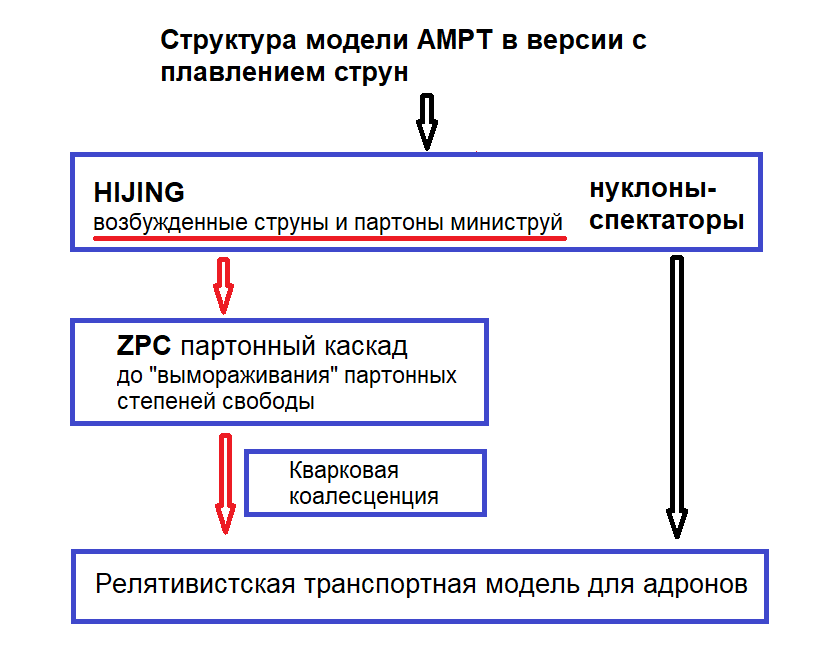
\includegraphics [width=0,5\linewidth]{Simulation/AMPT_SM.png}
		\caption{Иллюстрация структуры программного пакета AMPT в версии с плавлением струн} 
		\label{img:AMPT_sm}
	\end{figure}
	
	К моменту начала фазы адронизации, в столкновении присутствуют струны,  и партоны министруй.  
	Партоны министруй, образованных в жестких процессах, перед фрагментацией в адроны могут рассеиваться. Поскольку количество жестких столкновений в столкновении A+A примерно равно $A^{4/3}$ и растет с увеличением энергии столкновения, в то время как количество струн примерно равно A, влияние министруй увеличивается с ростом энергий. Однако для центральных столкновений Au+Au даже при 200 A ГэВ партоны министруй несут лишь около 1/3 суммарного поперечной энергии, поэтому влияние партонного рассеяния на конечную множественность частиц и спектры довольно мало 
	Приведенная выше картина сосуществования партонов и струн на начальной стадии столкновений тяжелых ионов высоких энергий вызывает сомнения, когда плотность энергии намного выше критической плотности для фазового перехода КХД. В этом случае ожидается, что струны расплавятся в партонные степени свободы. 
	И транспортная модель, и подход КХД высокой плотности предсказывают, что начальная плотность энергии образовавшегося вещества в центральных столкновениях Au+Au на RHIC более чем на порядок превышает критическую плотность энергии ($\sim$1 ГэВ/фм$^{3}$). Таким образом, сохранение струн в области высокой плотности энергии приводит к недооценке партонных эффектов в этих столкновениях. 
	Чтобы смоделировать плавление струны в областях с высокой плотностью энергии до партонов, модель AMPT модифицируется следующим образом. После моделирования начальных условий с помощью пакета HIJING (с выключенным эффектом гашения струй), происходит фрагментация струй в адроны с помощью пакета PYTHIA8, используещего модель Лунда, а затем образовавшиеся адроны конвертируются в партоны в соответствии с их ароматом и спином.
	Релятивиствские эффекты добавлены в модель путем введения времени формирования партонов, образующих министруи, которое зависит от их четырехимульса. 
	
	После того, как партоны перестают взамодействовать, начинается процесс их адрониации путем коалесценции. Модель коалесценции подразумевает, что два партона, находящихся рядом в фазовом пространстве формируют мезон, в то время как 3 кварка, находящихся рядом в фазовом просторанстве формируют барион. Поскольку инвариантная масса объединенных партонов формирует непрерывный 
	\subsection{Результаты}
	
\end{comment}
На Рисунке \ref{img:Ratio_same_sym} представлено сравнение значений $\pi^{-}/\pi^{+}$, $K^{-}/K^{+}$, $\bar{p}/p$, измеренных в $p$+Al, \heau, Cu+Au столкновениях при энергии 200 ГэВ и U+U столкновениях при энергии 193 ГэВ с предсказанями моделей PYTHIA8,3/ANGANTYR и AMPTsm. Величины отношений $\pi^{-}/\pi^{+}$, $K^{-}/K^{+}$, $\bar{p}/p$, полученные как с помощью программного пакета AMPTsm в версии с плавлением струн, так и с помощью программного пакета PYTHIA8,3/ANGANTYR не проявляют значимую зависимость от поперечного импульса и центральности. Полученные результаты моделирования совпадают как с экспериментальными данными, так и с предсказаниями термодинамической модели \cite{PPG026, ThermalisationRHIC}.

На Рисунках \ref{img:Ratio_LargeP2PI_sym}-\ref{img:Ratio_SmallK2PI_sym} представлены зависимости отношений $K^{+}/\pi^{+}$, $K^{-}/\pi^{-}$, $p/\pi^{+}$, $\bar{p}/\pi^{-}$ от поперечного импульса, измеренные в \pal, \heau, Cu+Au и U+U столкновениях, а также аналогичные зависимости, полученные с помощью программного пакета АMPTsm и  программного пакета PYTHIA8,3/ANGANTYR.
Величины отношений выходов $K^{+}/\pi^{+}$, $K^{-}/\pi^{-}$ проявляют слабую зависимость от центральности и совпадают с экспериментальными данными в пределах погрешностей. 

На основе результатов, представленных на Рисунке \ref{img:Ratio_LargeP2PI_sym} и Рисунке \ref{img:Ratio_SmallP2PI_sym} было установлено, что:

\begin{enumerate}
\item Предсказания значений $p/\pi^{+}$ и $\bar{p}/\pi^{-}$ моделью PYTHIA8,3/ANGANTYR во всех системах столкновений (\pal, \heau, Cu+Au, U+U) оказываются близки к результатам, полученным в \pp \ столкновениях. 
\item Модель AMPTsm позволяет качественно (но не количественно) описать рост значений $p/\pi^{+}$ и $\bar{p}/\pi^{-}$, наблюдаемый в эксперименте в центральных столкноыениях \heau, Cu+Au и U+U.
\item Величины $p/\pi^{+}$ и $\bar{p}/\pi^{-}$, полученные с помощью модели AMPTsm, численно не совпадают с экспериментально измеренными.
\item В системах столкновений, характеризующихся малыми значениями \Npart \ (\pal \ столкновения, а также периферические столкновения \heau, Cu+Au и U+U), значения $p/\pi^{+}$ и $\bar{p}/\pi^{-}$, полученные с помощью пакета AMPTsm, совпадают с предсказаниями модели PYTHIA8,3/ANGANTYR в пределах погрешностей.
\end{enumerate}

Согласно модели рекомбинации, \pT \ образующегося адрона складывается из \pT \ составляющих его кварков. Вследствие этого инвариантные \pT \ спектры, измеренные для барионов, сдвинуты в сторону больших \pT \ относительно инвариантных \pT \ спектров, измеренных для мезонов. В результате в области промежуточных \pT \ (2 ГэВ/$c < p_T < 4$ ГэВ/$c$) наблюдается увеличение выходов барионов по сравнению с выходами мезонов. Общее число барионов и мезонов, образующихся в процессах рекомбинации, пропорционально числу партонов внутри КГП. Следовательно, рост значений $p/\pi$ с увеличением центральности Cu+Au и U+U столкновений может означать растущее влияние процессов рекомбинации и увеличение числа партонов образующейся КГП. Согласие между предсказаниями модели рекомбинации и моделью фрагментации в столкновениях с малыми значениями \Npart \ (\pal \ столкновения, а также периферические столкновения \heau, Cu+Au и U+U) может указывать на то, что либо КГП в данных столкновениях не образуется, либо ее объем  недостаточен для наблюдаемого увеличения выхода барионов.


%Количество барионов и мезонов, пропорционально поперечному размеру КГП на стадии адронизации \cite{Thermal2}. Таким образом, можно сделать вывод, что объем образующейся в столкновении КГП, увеличивается с ростом центральнсти столкновения и, соответственно, с ростом \Npart. Совпадение предсказаний рекомбинационной модели и модели фрагментации  в столкновениях с $N_{part} \lesssim 10$ может свидетельствовать о недостаточности объема образующейся КГП для наблюдаемого увеличения выхода барионов.  На основании вышеизложенного сделан вывод о том, что в стокновениях, характеризующихся значениями $N_{part} \lesssim 10$ преобладает механизм фрагментации. При этом вклад рекомбинационного механизма усиливается с ростом \Npart, вызывая наблюдаемое увеличение выхода барионов. Тем не менее, модель рекомбинации, реализованная в пакете AMPT, не позволяет численно описать увеличение выходов протонов.

\begin{comment}
\begin{figure}[] 
	\centerfloat
	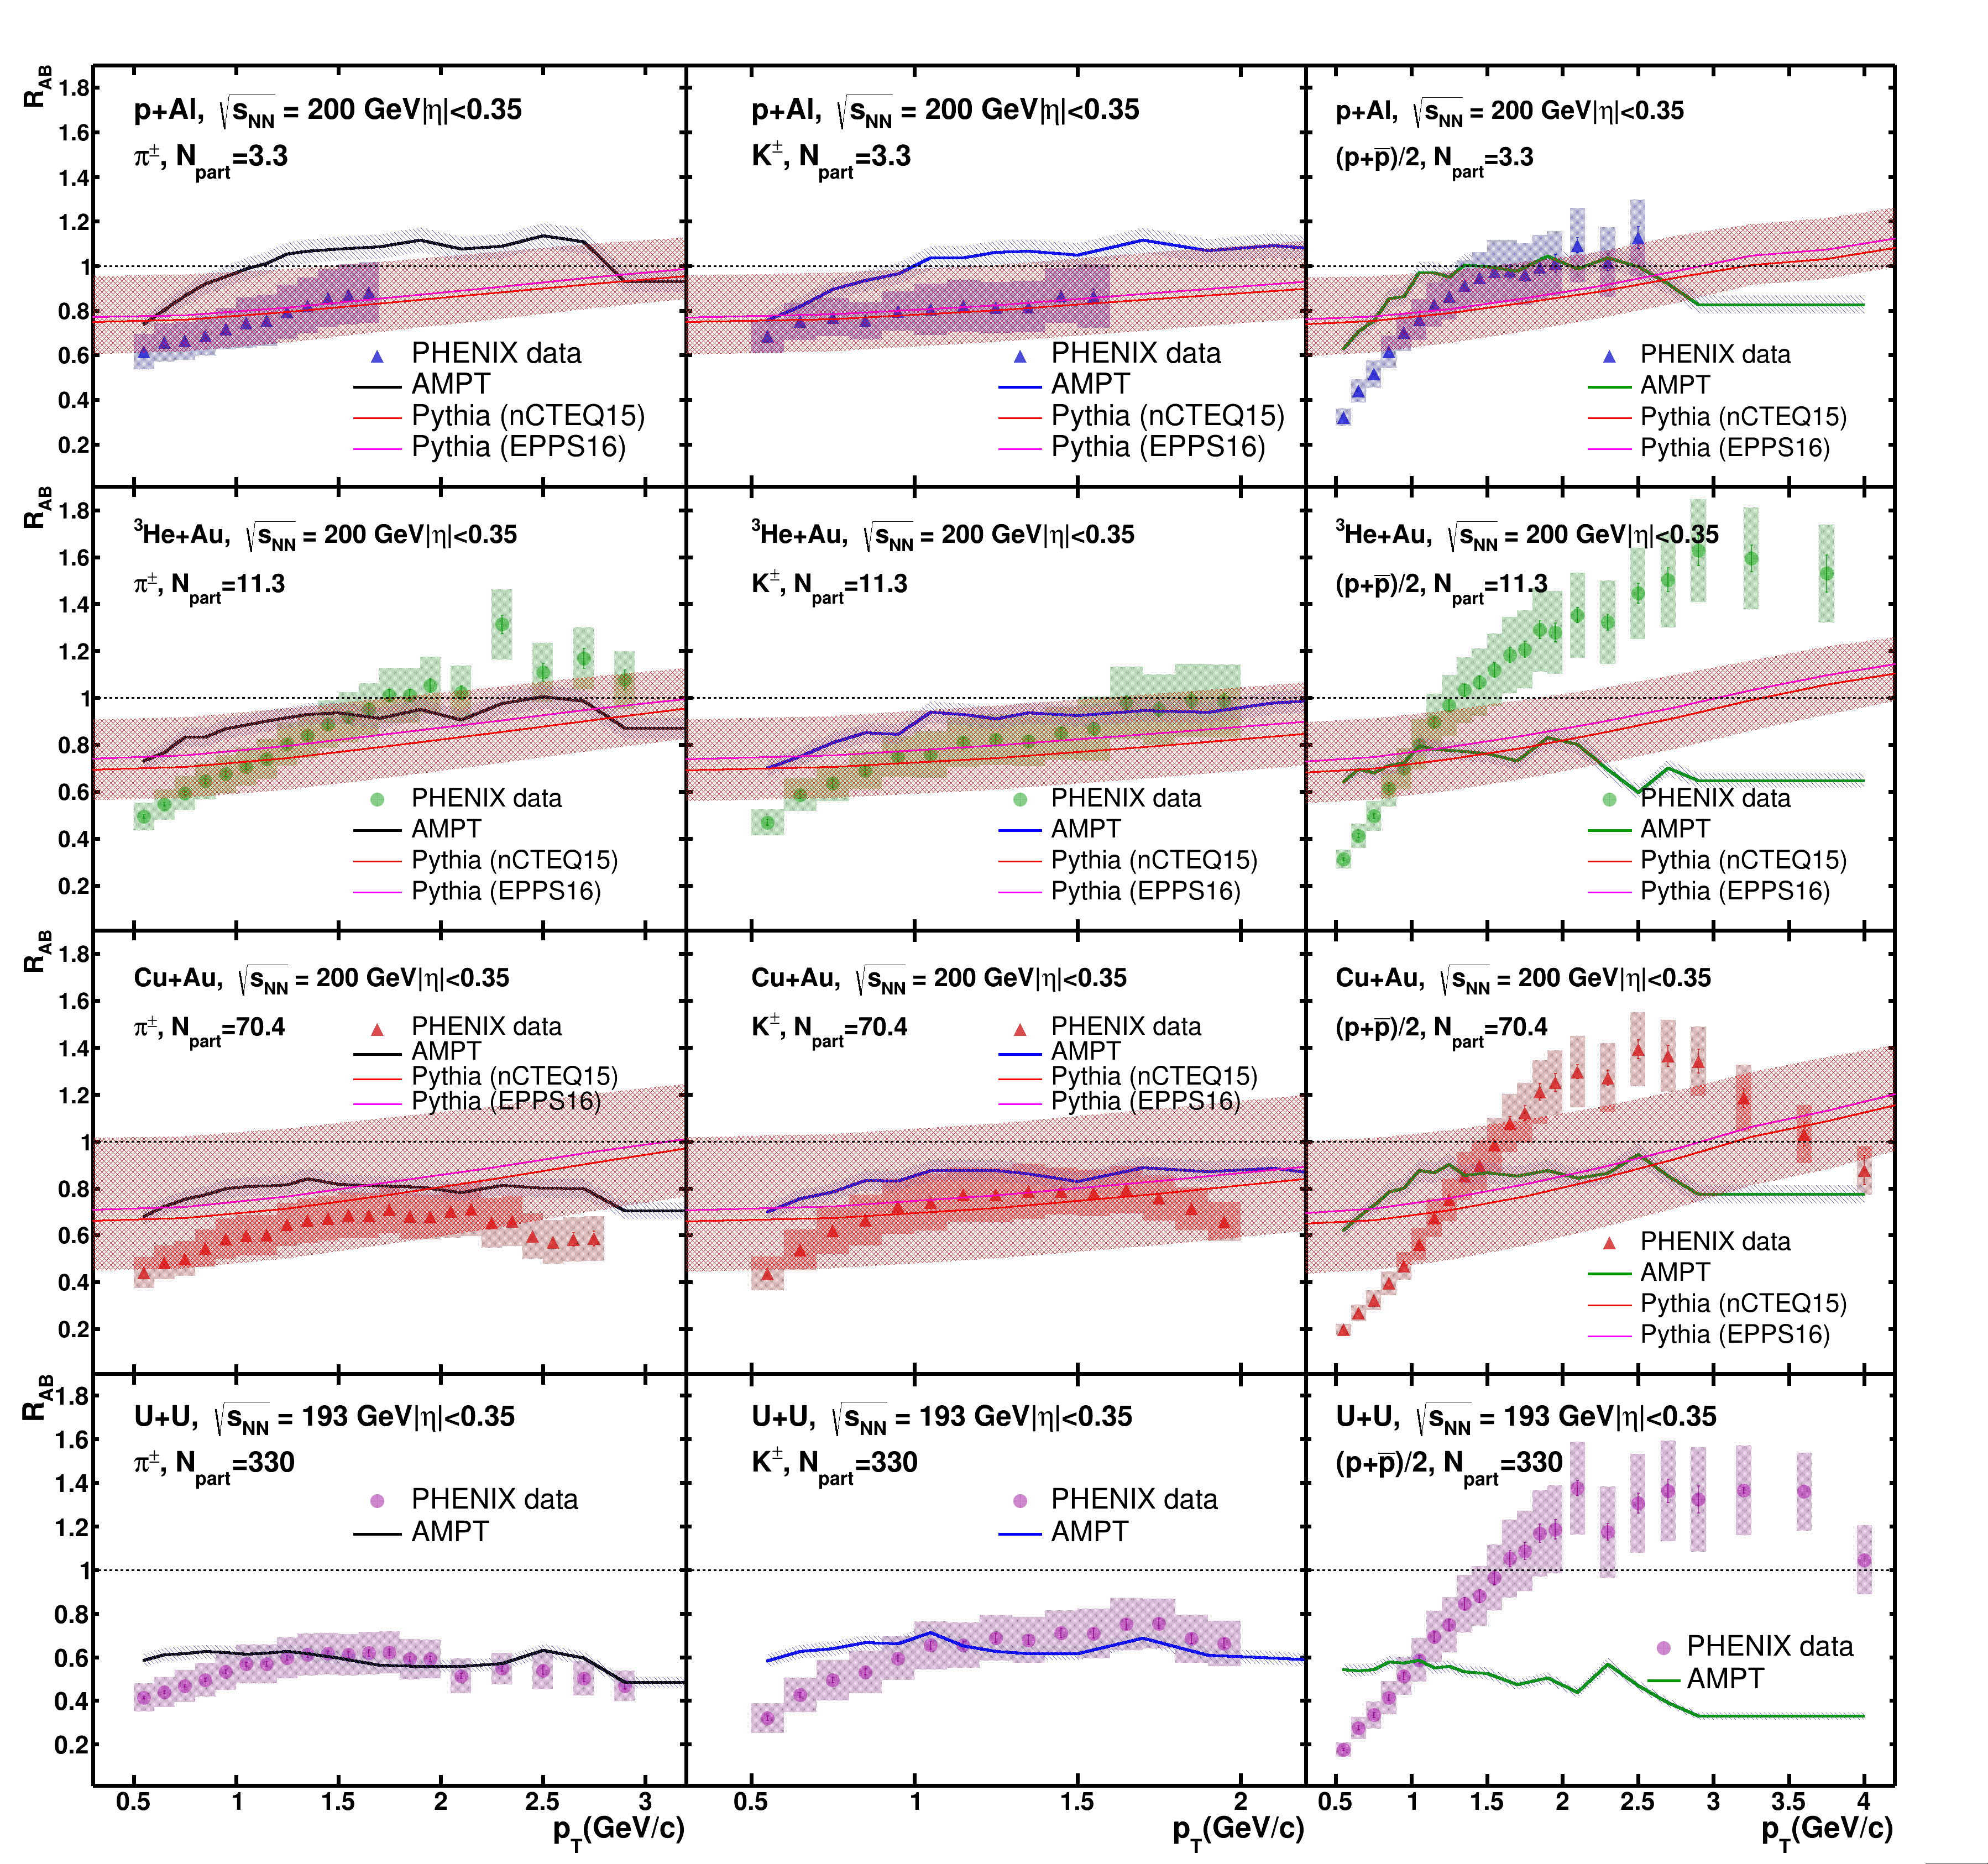
\includegraphics [width=1\linewidth]{Simulation/RAA_AMPT_Pythia.png}
	\caption{Сравнение факторов ядерной модификации (\rab), полученных для \pipm, \Kpm, \prot \ b \aprot \ в рамках фрагментационной (Pythia8) и рекомбинационной (AMPT) моделей, с экспериментальными результатами в различных центральностях \pal, \heau, Cu+Au и U+U столкновений. } 
	\label{img:RAA_sym}
\end{figure}
\end{comment}

\begin{figure}[] 
	\centerfloat
	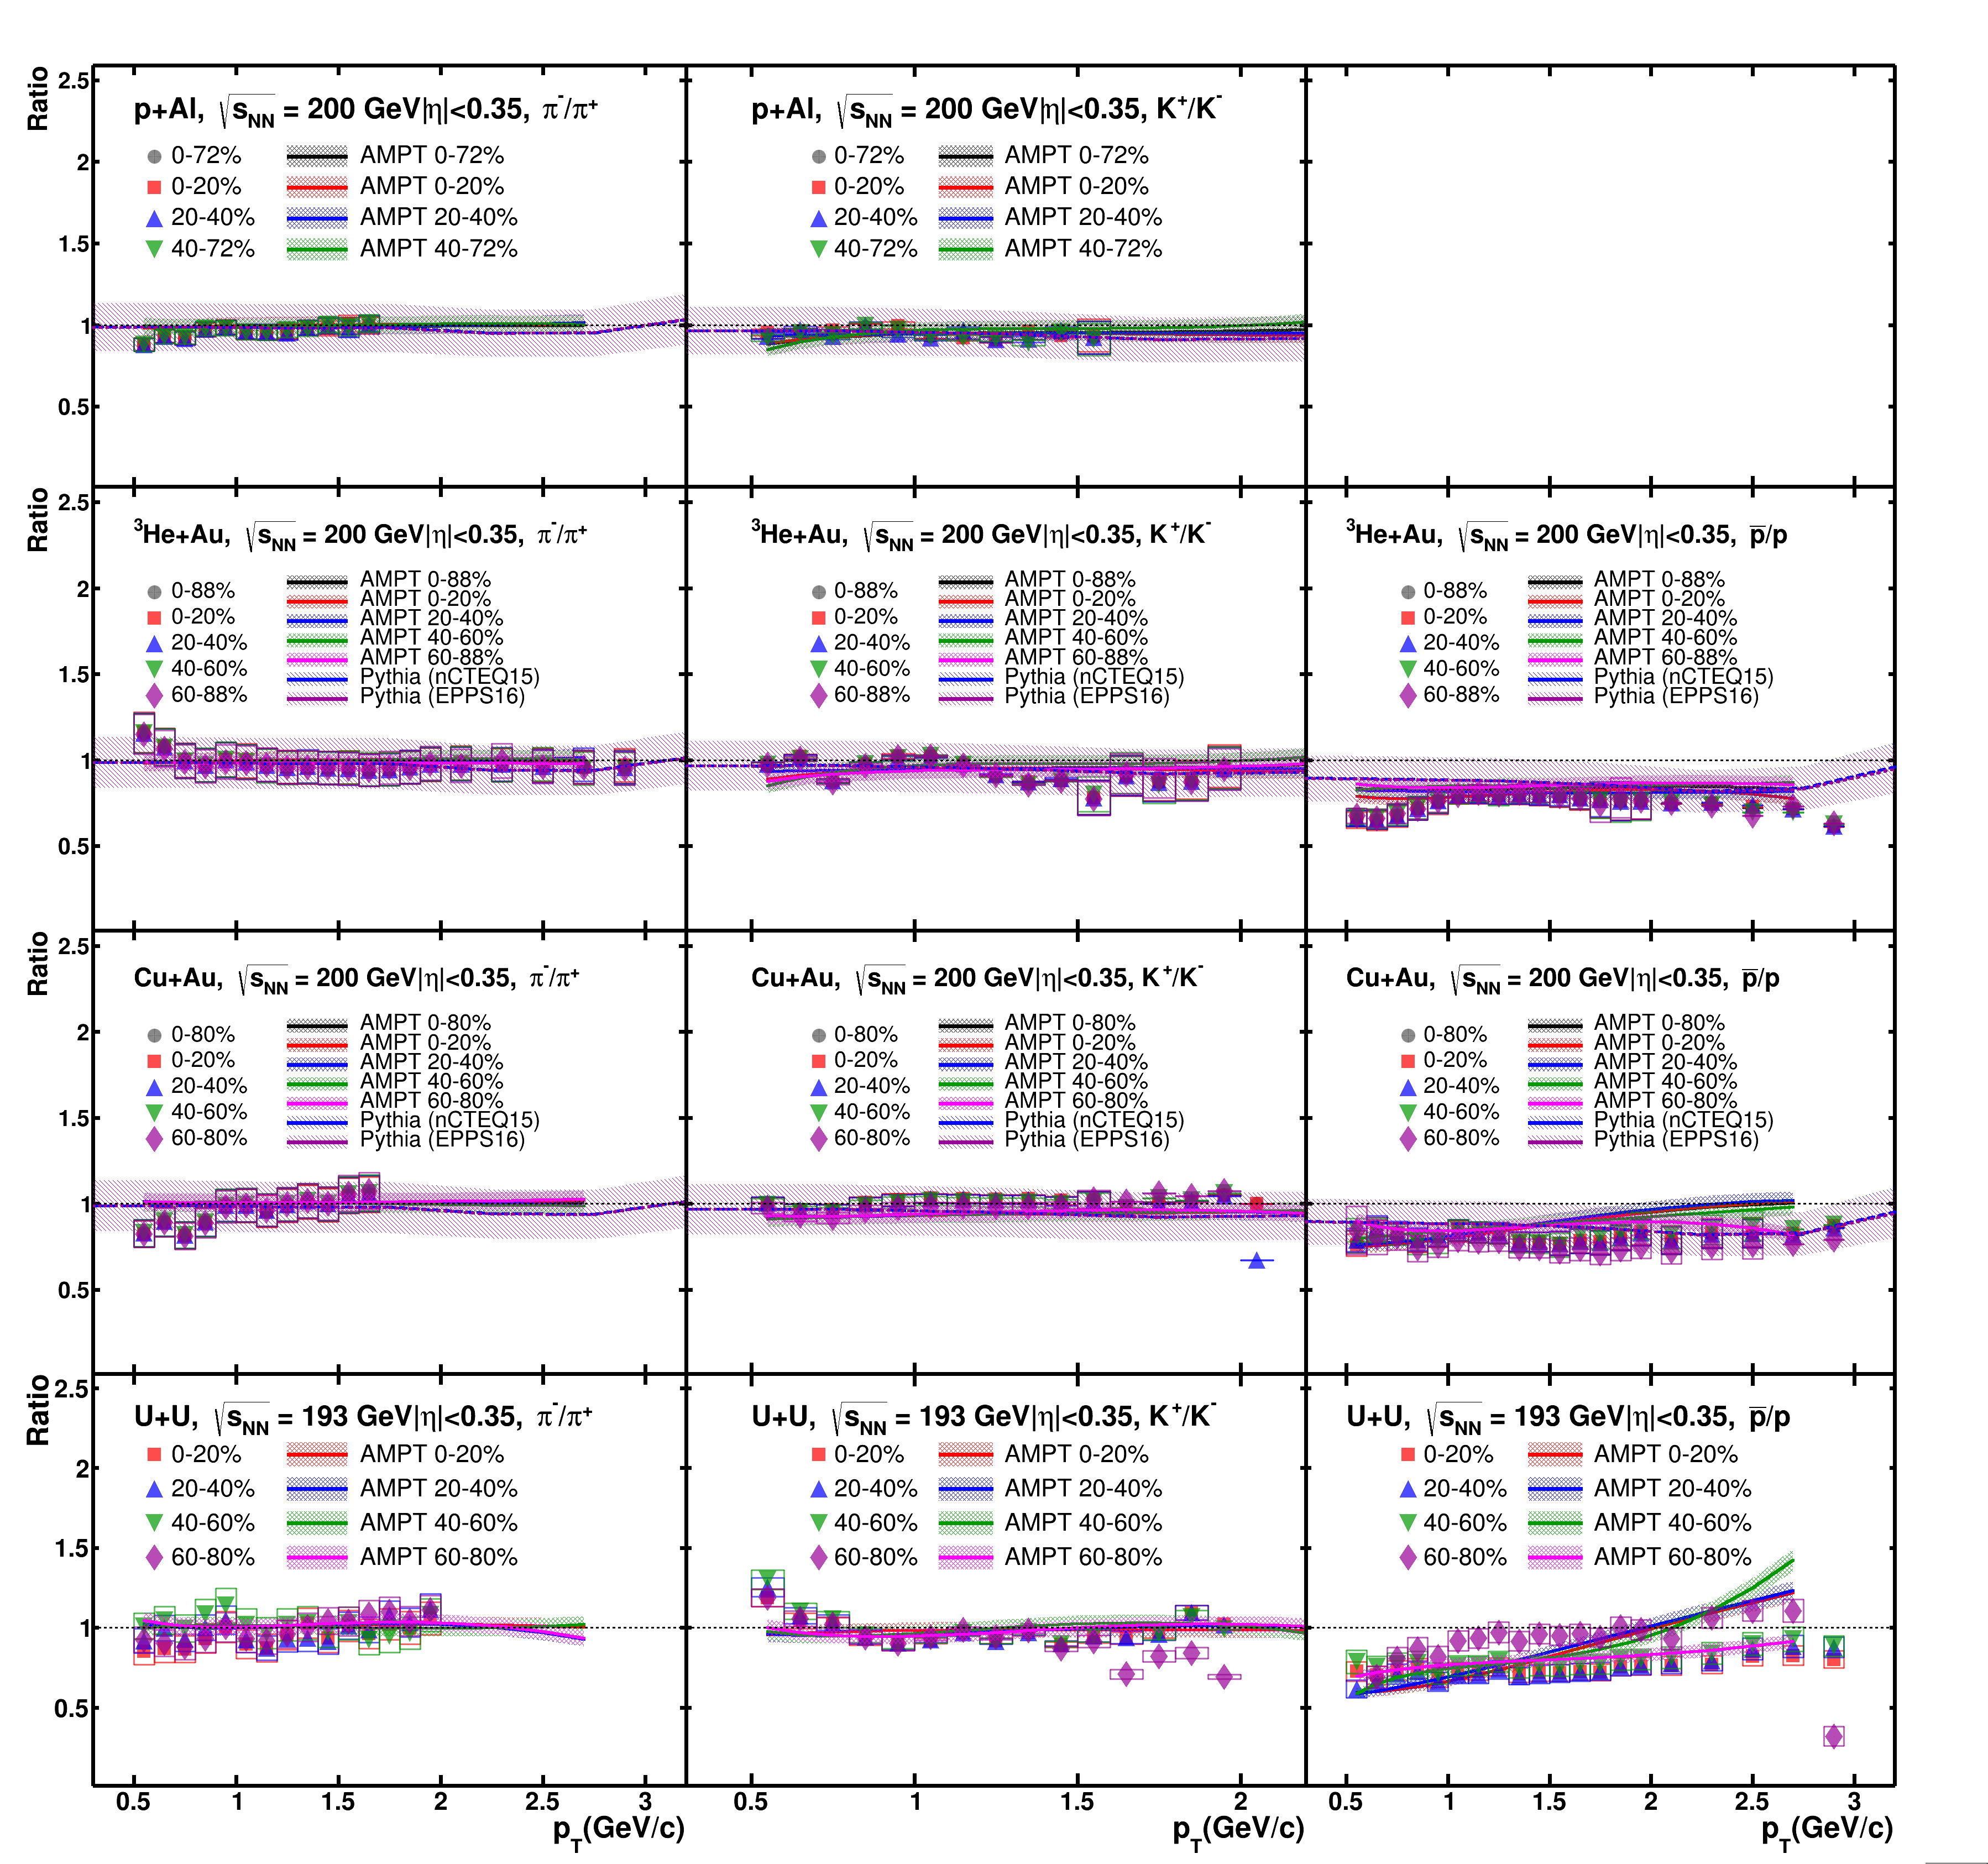
\includegraphics [width=1\linewidth]{Simulation/Ratio_same_AMPT_Pythia.png}
	\caption{Сравнение величин $\pi^{-}/\pi^{+}$, $K^{-}/K^{+}$, $\bar{p}/p$, полученных в рамках фрагментационной (Pythia8,3/ANGANTYR) и рекомбинационной (AMPTsm) моделей, с экспериментальными результатами в различных центральностях \pal, \heau, Cu+Au и U+U столкновений.} 
	\label{img:Ratio_same_sym}
\end{figure}


\begin{figure}[] 
	\centerfloat
	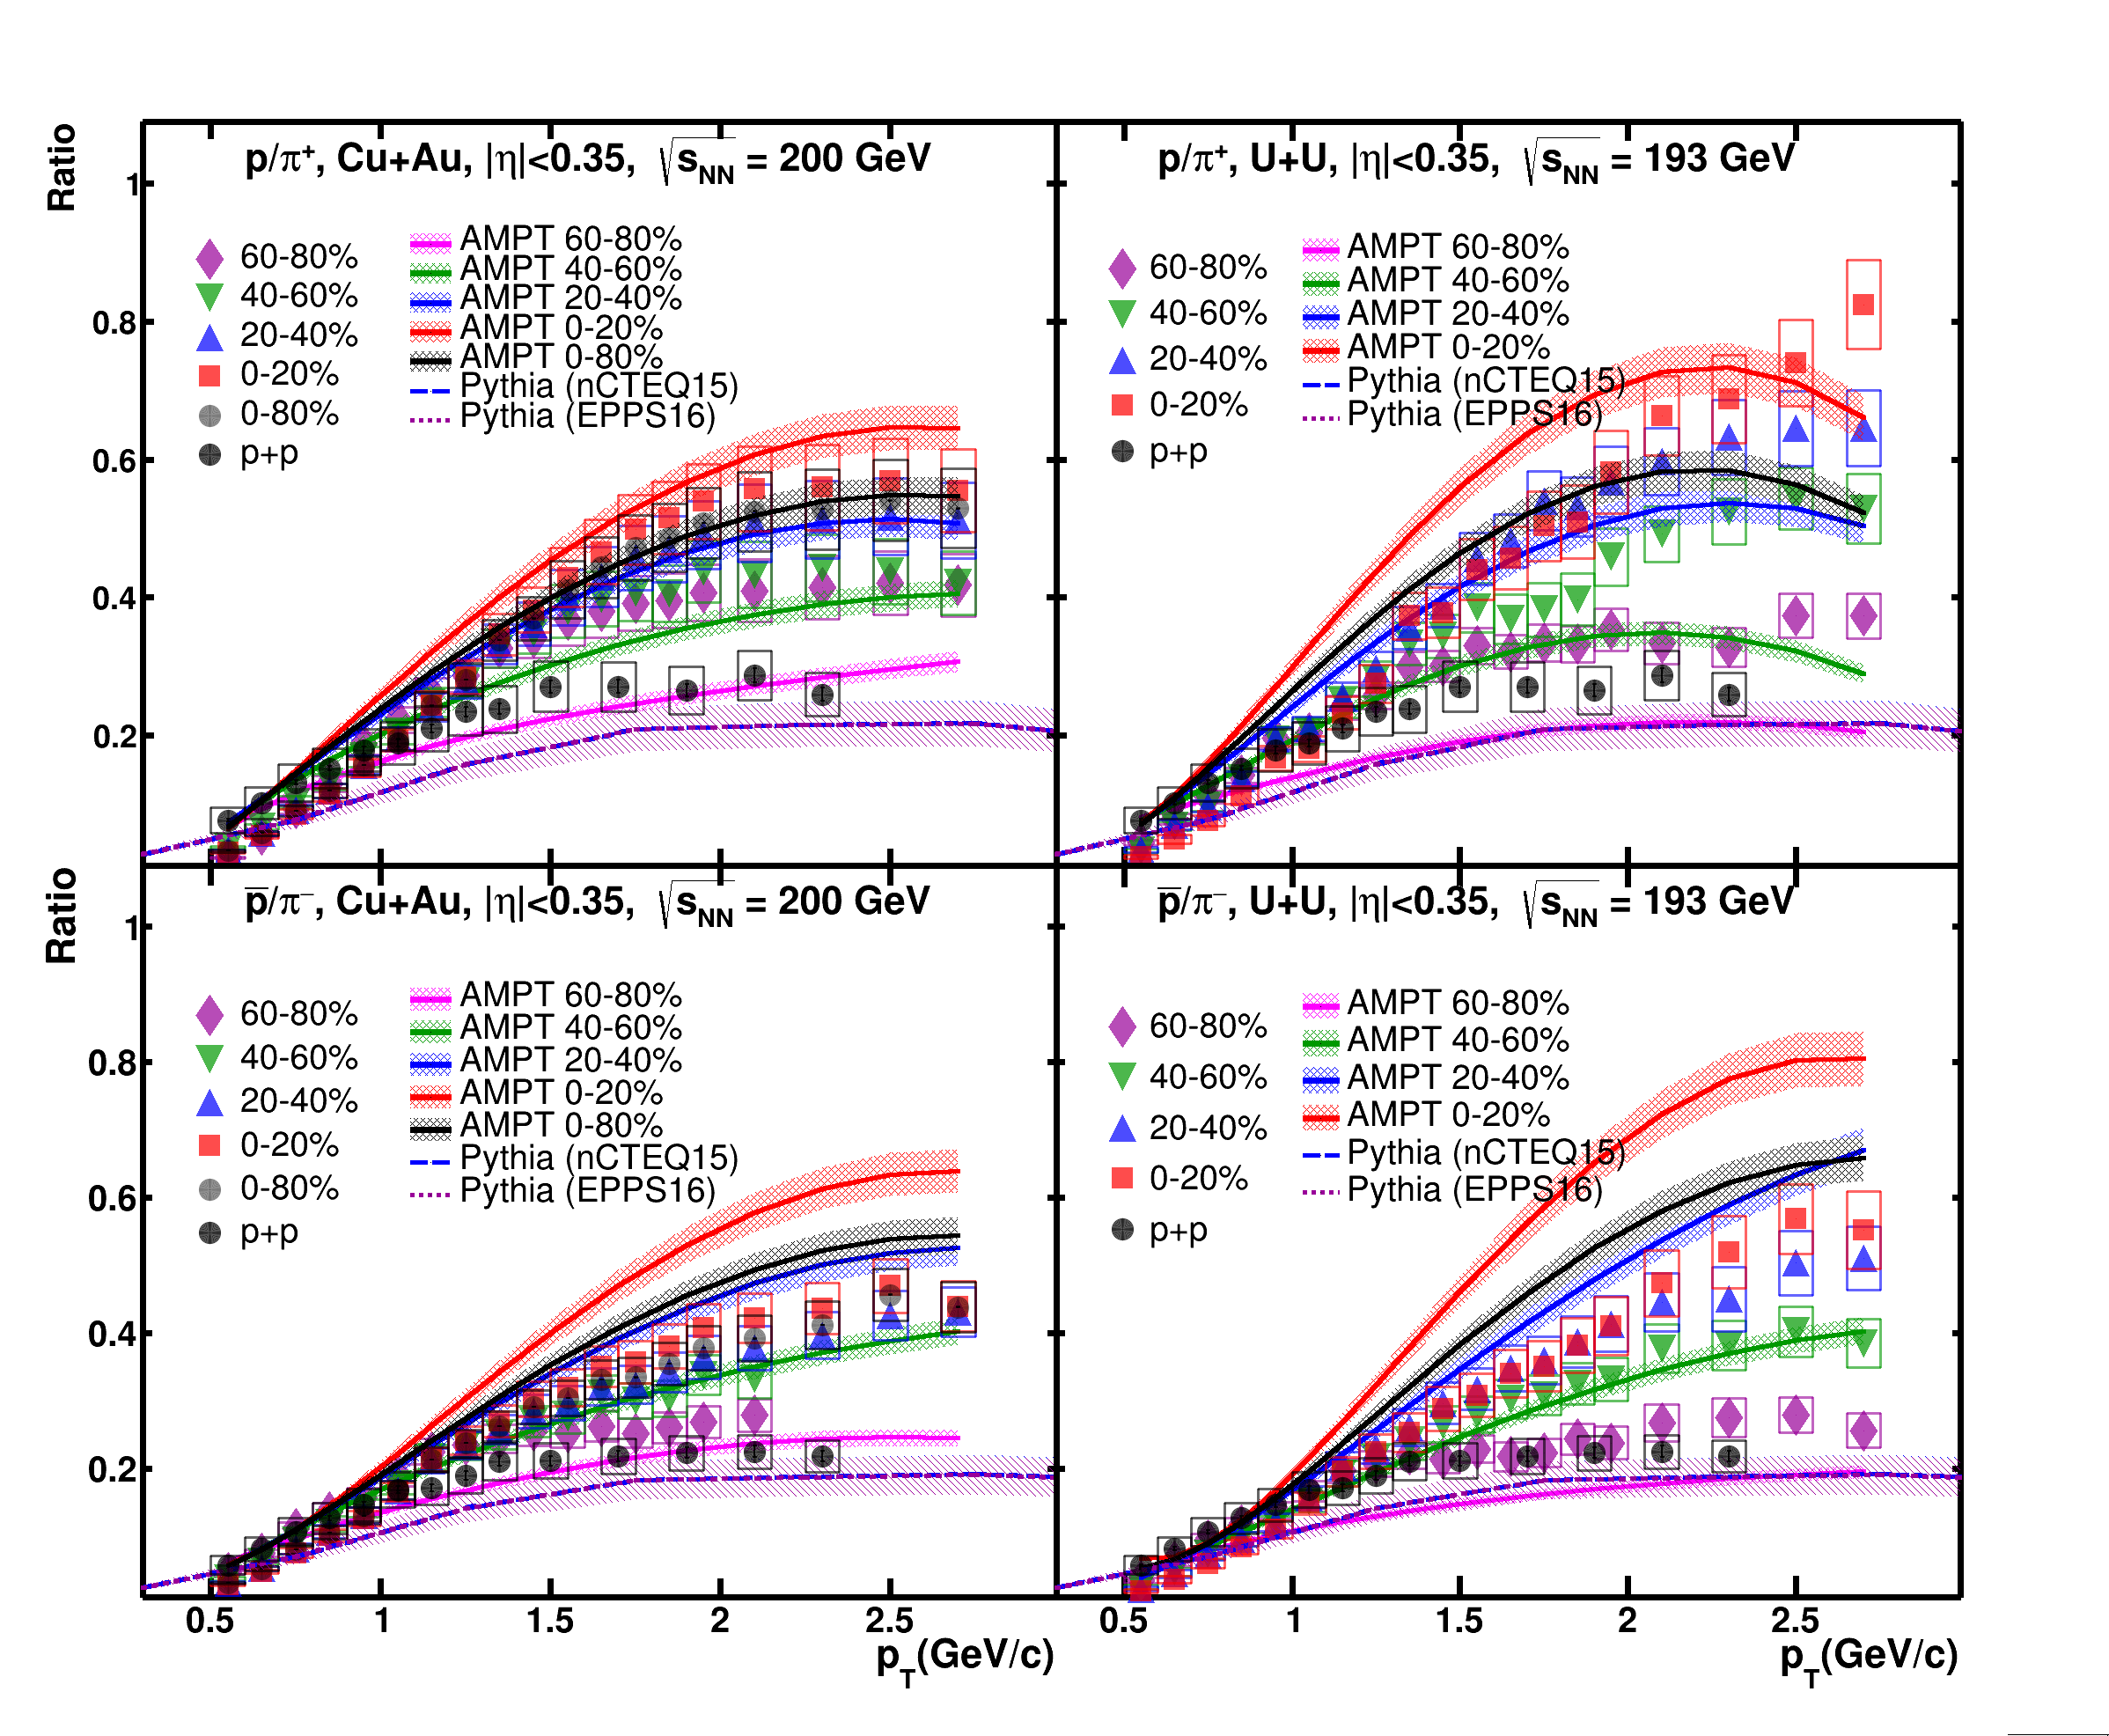
\includegraphics [width=0.6\linewidth]{Simulation/Ratios_AMPT_large_p2pi.png}
	\caption{Сравнение величин $p/\pi^{+}$ и $\bar{p}/\pi^{+}$, полученных с помощью пакета Pythia8,3/ANGANTYR, реализующего адронизацию посредством фрагментационных процессов, и  пакета AMPTsm, учитывающего процессы рекомбинации, с экспериментальными результатами в различных центральностях Cu+Au и U+U столкновений.} 
	\label{img:Ratio_LargeP2PI_sym}
\end{figure}

\begin{figure}[] 
	\centerfloat
	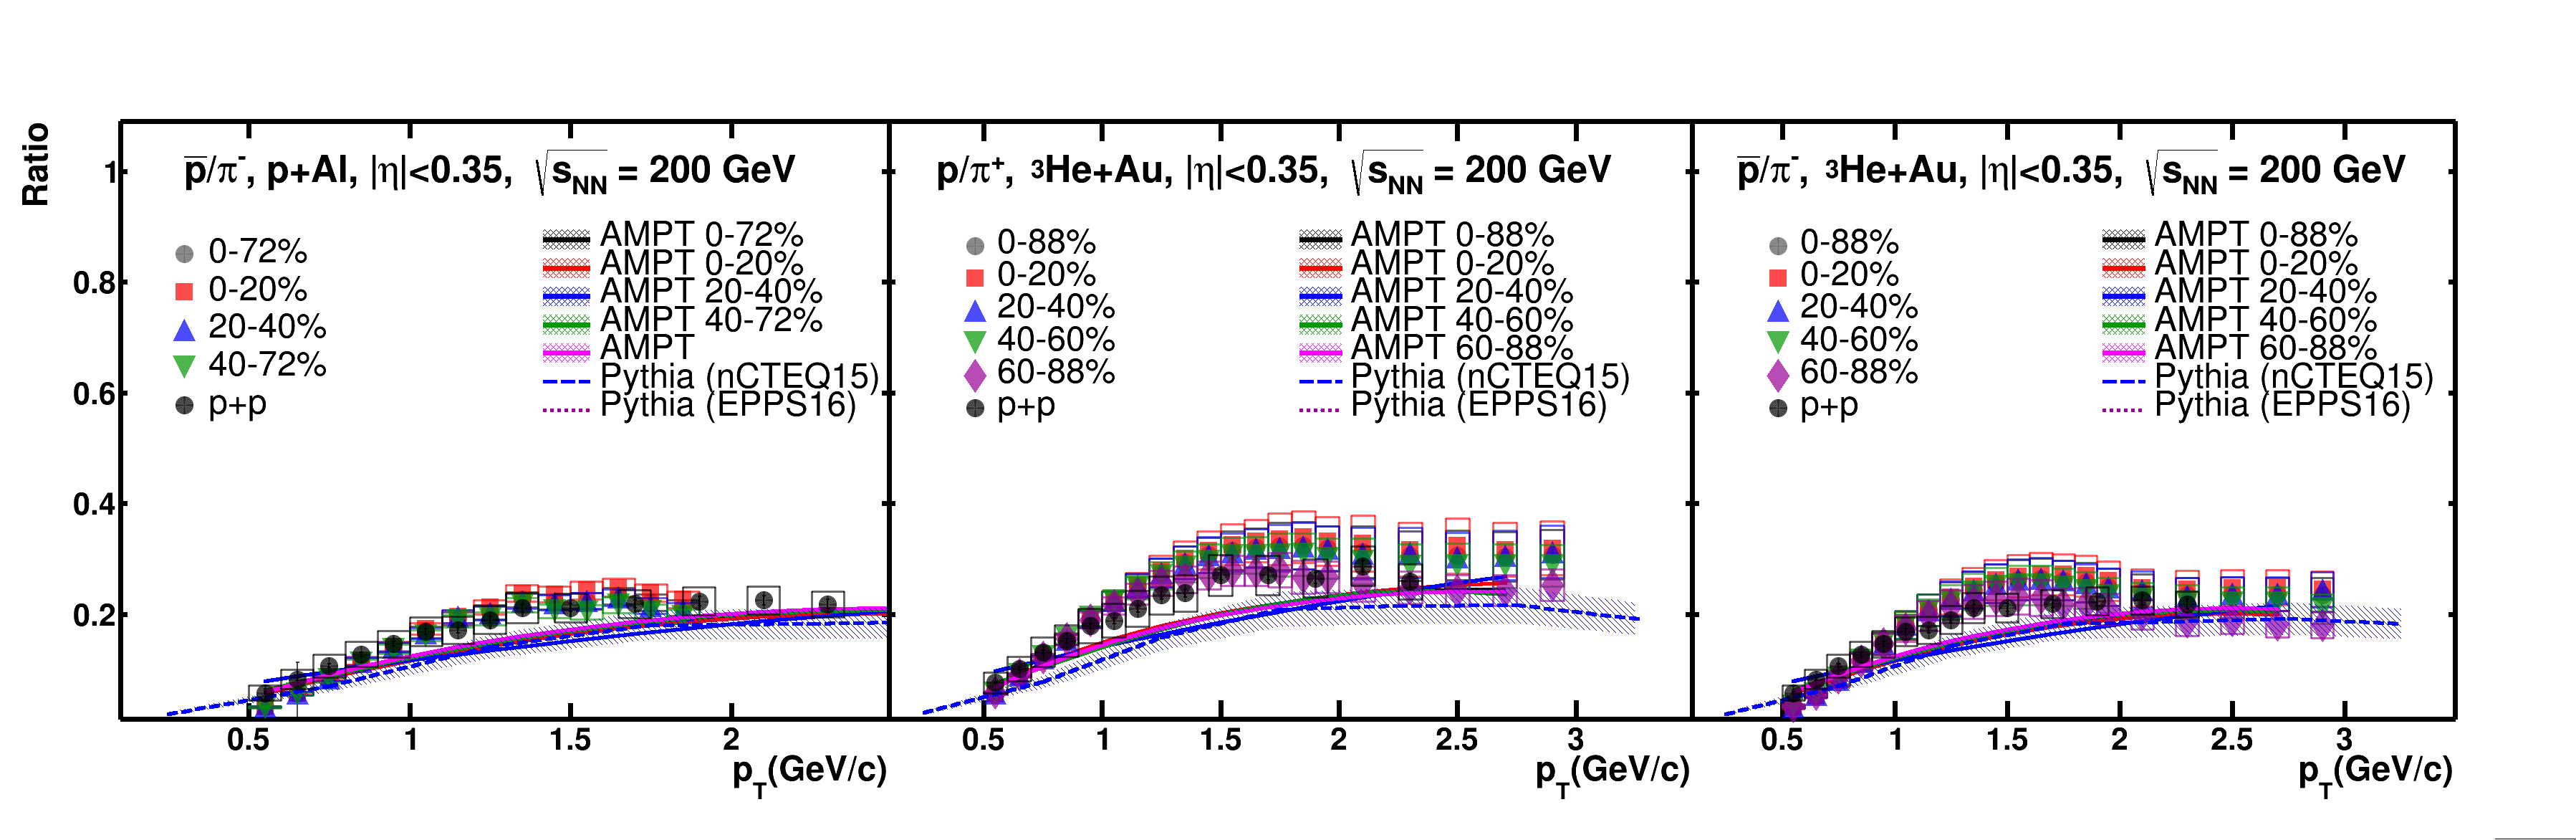
\includegraphics [width=1\linewidth]{Simulation/Ratios_AMPT_small_p2pi.png}
	\caption{Сравнение величин $p/\pi^{+}$ и $\bar{p}/\pi^{+}$, полученных с помощью пакета Pythia8,3/ANGANTYR, реализующего адронизацию посредством фрагментационных процессов, и  пакета AMPTsm, учитывающего процессы рекомбинации, с экспериментальными результатами в различных центральностях \pal \ и \heau \ столкновений.} 
	\label{img:Ratio_SmallP2PI_sym}
\end{figure}

\begin{figure}[] 
	\centerfloat
	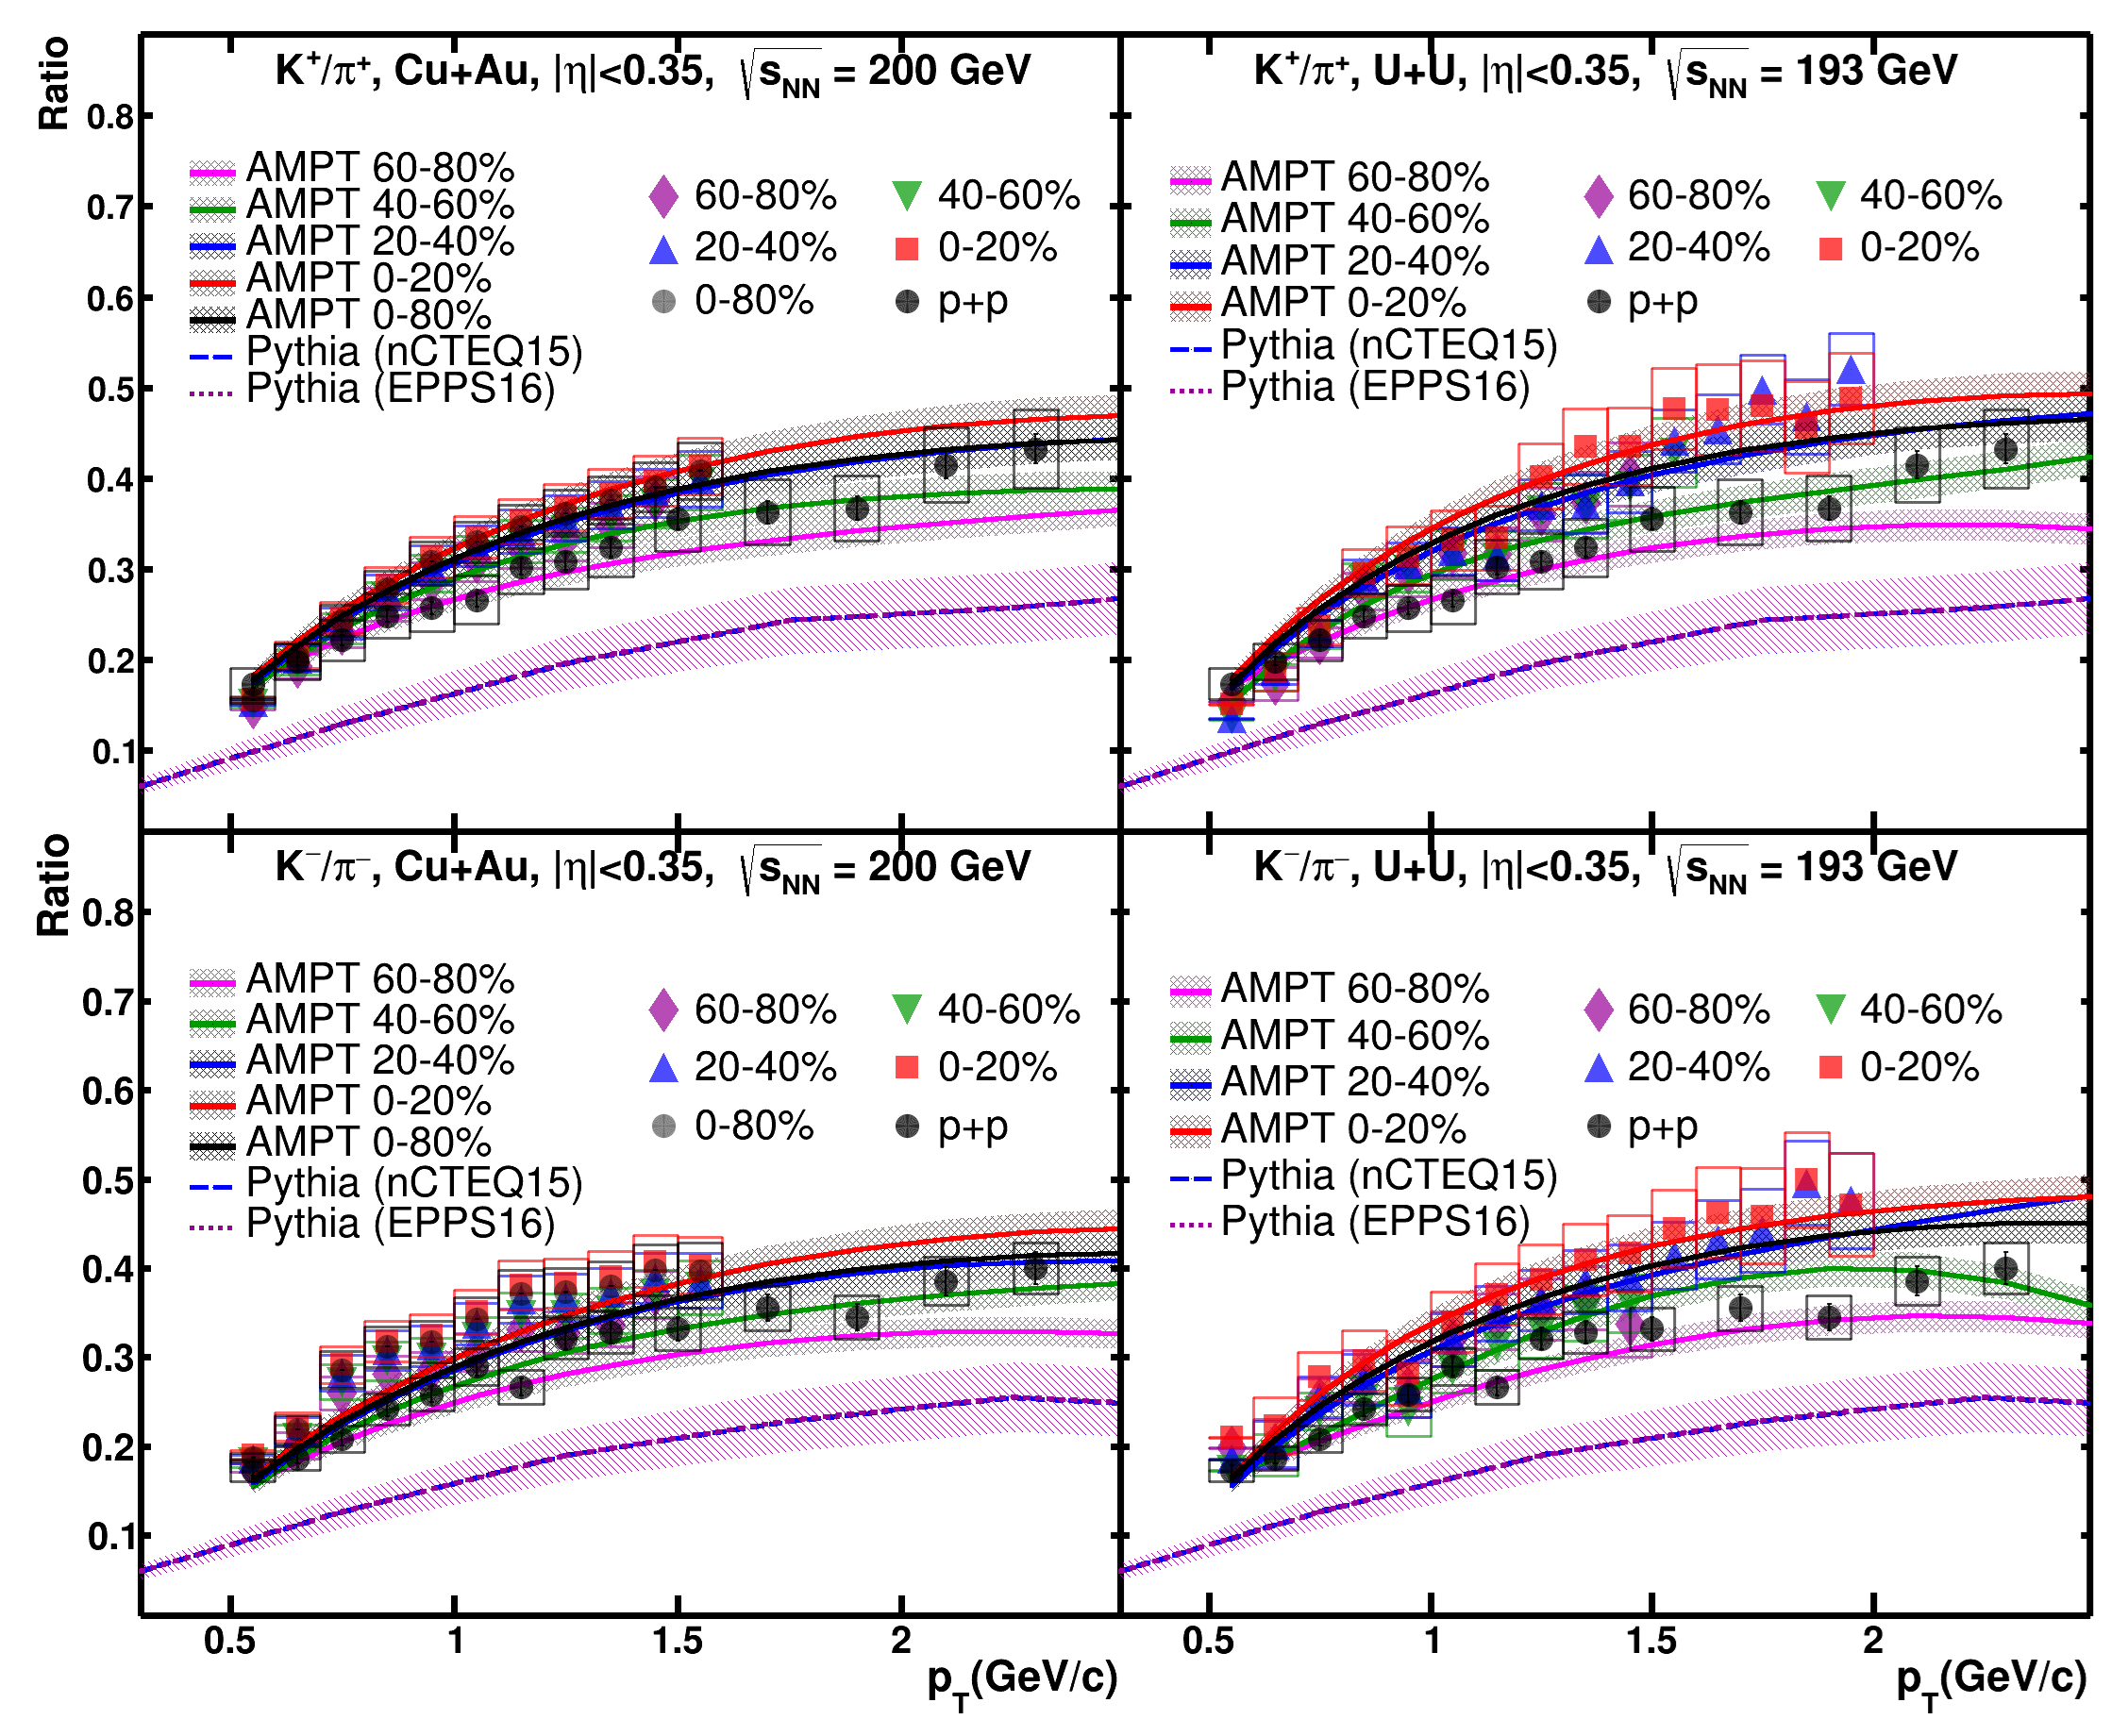
\includegraphics [width=0.6\linewidth]{Simulation/Ratios_AMPT_large_K2pi.png}
	\caption{Сравнение величин $K^{+}/\pi^{+}$ и $K^{-}/\pi^{-}$, полученных с помощью пакета Pythia8,3/ANGANTYR, реализующего адронизацию посредством фрагментационных процессов, и  пакета AMPTsm, учитывающего процессы рекомбинации, с экспериментальными результатами в различных центральностях Cu+Au и U+U столкновений.} 
	\label{img:Ratio_LargeK2PI_sym}
\end{figure}

\begin{figure}[] 
	\centerfloat
	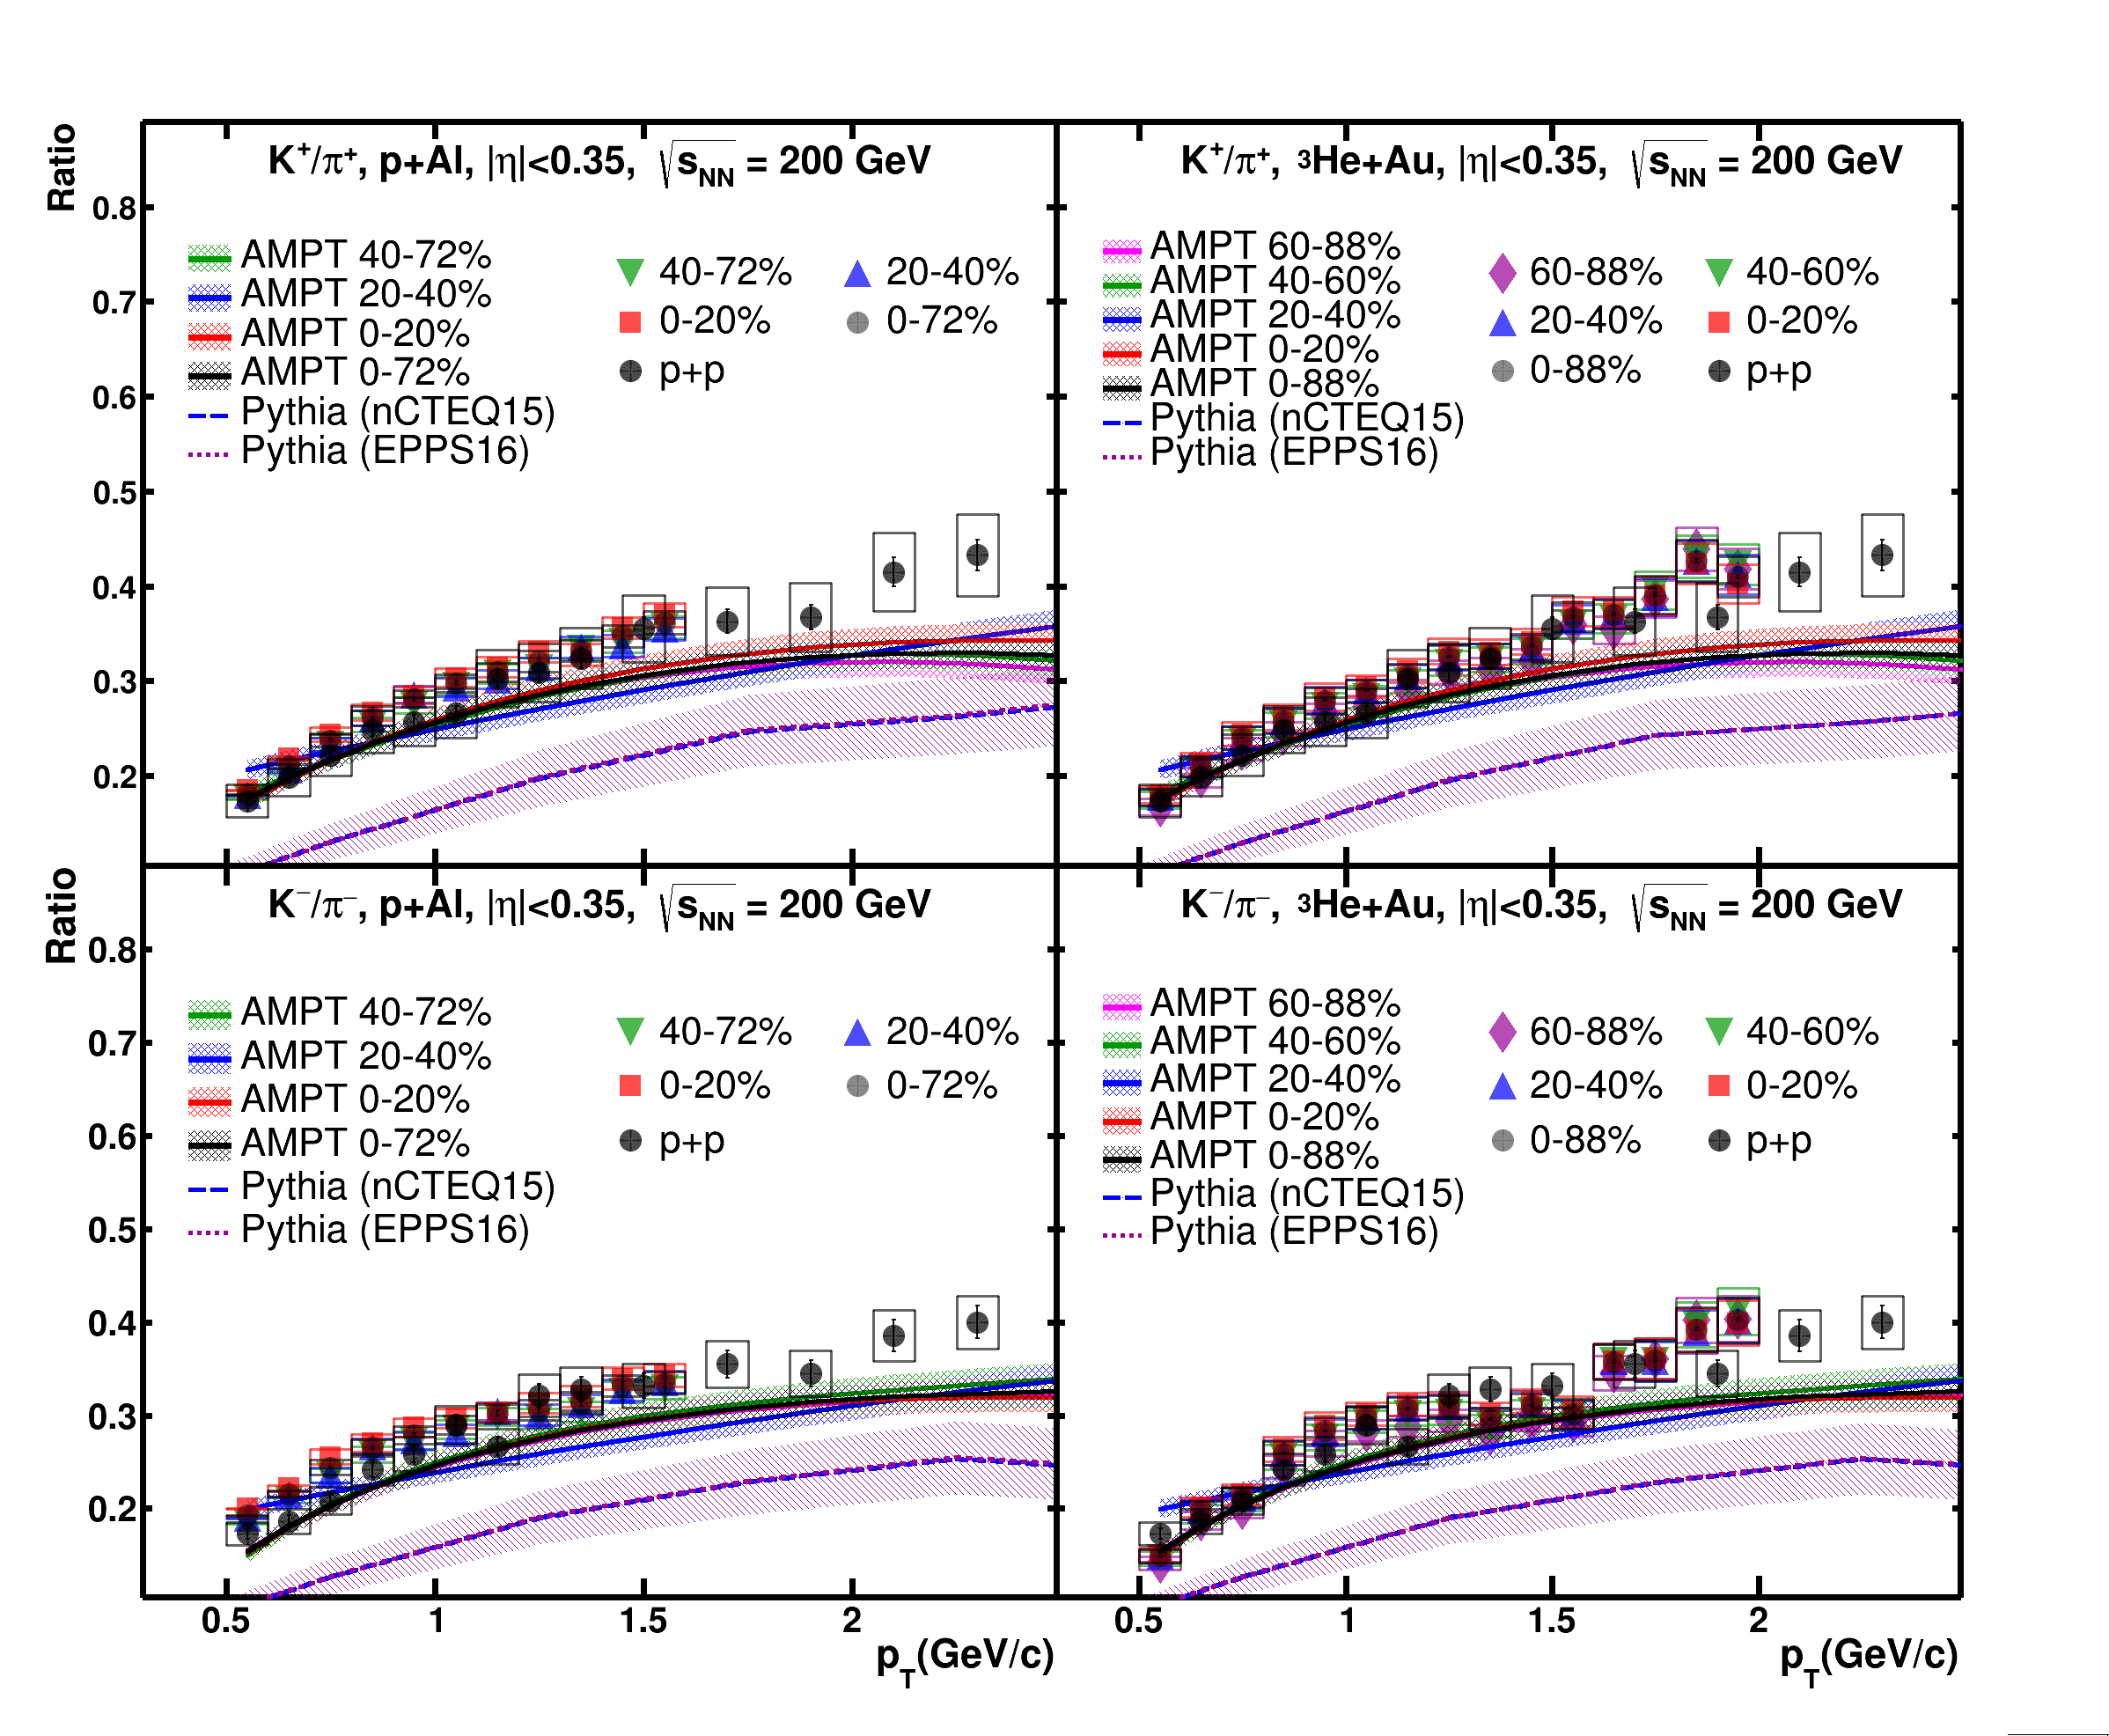
\includegraphics [width=0.6\linewidth]{Simulation/Ratios_AMPT_small_K2pi.png}
	\caption{Сравнение величин $K^{+}/\pi^{+}$ и $K^{-}/\pi^{-}$, полученных с помощью пакета Pythia8,3/ANGANTYR, реализующего адронизацию посредством фрагментационных процессов, и  пакета AMPTsm, учитывающего процессы рекомбинации, с экспериментальными результатами в различных центральностях \pal \ и \heau \ столкновений.} 
	\label{img:Ratio_SmallK2PI_sym}
\end{figure}           % Глава 5
\chapter*{Заключение}                       % Заголовок
\addcontentsline{toc}{chapter}{Заключение}  % Добавляем его в оглавление

%% Согласно ГОСТ Р 7.0.11-2011:
%% 5.3.3 В заключении диссертации излагают итоги выполненного исследования, рекомендации, перспективы дальнейшей разработки темы.
%% 9.2.3 В заключении автореферата диссертации излагают итоги данного исследования, рекомендации и перспективы дальнейшей разработки темы.
%% Поэтому имеет смысл сделать эту часть общей и загрузить из одного файла в автореферат и в диссертацию:

Основные результаты работы заключаются в следующем.
%% Согласно ГОСТ Р 7.0.11-2011:
%% 5.3.3 В заключении диссертации излагают итоги выполненного исследования, рекомендации, перспективы дальнейшей разработки темы.
%% 9.2.3 В заключении автореферата диссертации излагают итоги данного исследования, рекомендации и перспективы дальнейшей разработки темы.
Представлены измерения инвариантных спектров по поперечному импульсу, факторов ядерной модификации, измеренные для идентифицируемых заряженных адронов ($\pi^\pm$, $K^\pm$, $p$, $\bar{p}$), а также отношений выходов адронов -- \pim/\pip, \Km/\Kp, \prot/\aprot, \prot/\pip, \aprot/\pim, \Kp/\pip, \Km/\pim.

На основе анализа инвариантных \pt \ и \mt \ спектров были получены значения температуры химического вымораживания $T_{0}$ и средней скорости коллективного потока частиц $\left< u_T \right>$ как функций от количества нуклонов-участников \Npart.
Величина $T_{0}\approx170$ МэВ и является постоянной относительно значений \Npart, в то время как величина \ut \ увеличивается с увеличением значений \Npart. Данный результат может свидетельствовать о том, что в столкновениях, характеризующихся большими значениями $\left<N_{part}\right>$ (центральные Cu+Au, Au+Au, U+U столкновения), коллективные эффекты выражены сильнее, чем в столкновениях с малыми значениями $N_{part}$ (\pal, \heau \ столкновения).

Сравнение факторов ядерной модификации идентифицированных заряженных адронов показало, что значения \rab, измеренные в системах с разной геометрией (\dau, \heau, Cu+Au, Au+Au и U+U) совпадают при одинаковых значениях \Npart.
Сделан вывод, что рождение идентифицированных заряженных адронов не зависит от геометрии и размера системы столкновения и определяется лишь размером области перекрытия ядер, характеризующейся значением \Npart.

В центральных столкновениях \heau, Cu+Au, U+U был обнаружен эффект увеличенного выхода протонов и антипротонов, что может быть объяснено доминированием вклада процессов рекомбинации в образовние иднентифицируемых заряженных адронов в диапазоне малых и промежуточных поперечных импульсов ($p_{T}<4$ ГэВ/$c$). 
В \pal \ столкновениях, а также в периферических столкновениях \heau, Cu+Au, U+U эффект увеличенного выхода протонов и антипротонов не наблюдался, что может быть интерпретировано как доминирование вклада процессов фрагментации в образовние иднентифицируемых заряженных адронов в диапазоне промежуточных поперечных импульсов (2 ГэВ/$c$ $<p_{T}<4$ ГэВ/$c$).

Полученные значения инвариантных спектров заряженных адронов могут быть использованы для уточнения параметров теоретических моделей, реализованных в пакетах прикладных программ, таких как  AMPT, HIJING, PHSD и др. В частности, для уточнения радиуса рекомбинации в рекомбинационных моделях, реализованных в таких программных пакетах как AMPT, PHSD.

Автор выражает глубочайшую признательность научному руководителю, доктору физико-математических наук, профессору, Бердникову Я.А. и благодарит его за помощь в подготовке диссертации и публикаций, а также поддержку в течение всего периода обучения и работы в университете. Также автор благодарит Котова Д.О. за помощь в подготовке публикаций и обсуждение научных результатов. Автор сердечно благодарит всю группу эффективной молодежи кафедры ядерной физики СПбПУ, коллег Митранкову М.М., Митранкова Ю.М., Борисова В.С., Егорова А.Ю. за помощь и поддержку во время выполнения работы.
Огромная благодарность бабушке, подруге Цыцыной А.Р. и Галинскому В.А. за поддержку и веру в меня.

      % Заключение
\printnomenclature[3.5cm] % Значение ширины столбца с обозначениями стоит подбирать вручную
        % Список сокращений и условных обозначений
\chapter*{Словарь терминов}             % Заголовок
\addcontentsline{toc}{chapter}{Словарь терминов}  % Добавляем его в оглавление

\textbf{TeX} "--- Cистема компьютерной вёрстки, разработанная американским профессором информатики Дональдом Кнутом

\textbf{Панграмма} "--- Короткий текст, использующий все или почти все буквы алфавита
      % Словарь терминов
\clearpage                                  % В том числе гарантирует, что список литературы в оглавлении будет с правильным номером страницы
%\hypersetup{ urlcolor=black }               % Ссылки делаем чёрными
%\providecommand*{\BibDash}{}                % В стилях ugost2008 отключаем использование тире как разделителя 
\urlstyle{rm}                               % ссылки URL обычным шрифтом
\insertbibliofull                          % Подключаем Bib-базы
\urlstyle{tt}                               % возвращаем установки шрифта ссылок URL
%\hypersetup{ urlcolor={urlcolor} }          % Восстанавливаем цвет ссылок      % Список литературы
\clearpage
\phantomsection
\addcontentsline{toc}{chapter}{\listfigurename}
\listoffigures									% Список изображений
\newpage

\clearpage
\phantomsection
\addcontentsline{toc}{chapter}{\listtablename}
\listoftables									% Список таблиц
\newpage           % Списки таблиц и изображений (иллюстративный материал)

\setcounter{totalchapter}{\value{chapter}} % Подсчёт количества глав

%%% Настройки для приложений
\appendix
% Оформление заголовков приложений ближе к ГОСТ:
\setlength{\midchapskip}{20pt}
\renewcommand*{\afterchapternum}{\par\nobreak\vskip \midchapskip}
\renewcommand\thechapter{\Asbuk{chapter}} % Чтобы приложения русскими буквами нумеровались

\appendix
%% Правка оформления ссылок на приложения:
%http://tex.stackexchange.com/questions/56839/chaptername-is-used-even-for-appendix-chapters-in-toc
%http://tex.stackexchange.com/questions/59349/table-of-contents-with-chapter-and-appendix
%% требует двойной компиляции
\addtocontents{toc}{\def\protect\cftchappresnum{\appendixname{} }%
\setlength{\cftchapnumwidth}{\widthof{\cftchapfont\appendixname~Ш\cftchapaftersnum}}%
}
%% Оформление заголовков приложений ближе к ГОСТ:
\sectionformat{\chapter}[display]{% Параметры заголовков разделов в тексте
    label=\chaptertitlename\ \thechapter,% (ГОСТ Р 2.105, 4.3.6)
    labelsep=20pt,
}
\renewcommand\thechapter{\Asbuk{chapter}} % Чтобы приложения русскими буквами нумеровались
   % Предварительные настройки для правильного подключения Приложений
\chapter{Примеры вставки листингов программного кода} \label{AppendixA}

Для крупных листингов есть два способа. Первый красивый, но в нём могут быть проблемы с поддержкой кириллицы (у вас может встречаться в комментариях и
печатаемых сообщениях), он представлен на листинге~\ref{list:hwbeauty}.
\begin{ListingEnv}[!h]% настройки floating аналогичны окружению figure
%    \captionsetup{format=tablenocaption}% должен стоять до самого caption
    \caption{Программа “Hello, world” на \protect\cpp}
    % далее метка для ссылки:
    \label{list:hwbeauty}
    % окружение учитывает пробелы и табуляции и применяет их в сответсвии с настройками
    \begin{lstlisting}[language={[ISO]C++}]
	#include <iostream>
	using namespace std;

	int main() //кириллица в комментариях при xelatex и lualatex имеет проблемы с пробелами
	{
		cout << "Hello, world" << endl; //latin letters in commentaries
		system("pause");
		return 0;
	}
    \end{lstlisting}
\end{ListingEnv}%
Второй не такой красивый, но без ограничений (см.~листинг~\ref{list:hwplain}).
\begin{ListingEnv}[!h]
    \caption{Программа “Hello, world” без подсветки}
    \label{list:hwplain}
    \begin{Verb}
        
        #include <iostream>
        using namespace std;
        
        int main() //кириллица в комментариях
        {
            cout << "Привет, мир" << endl;
        }
    \end{Verb}
\end{ListingEnv}

Можно использовать первый для вставки небольших фрагментов
внутри текста, а второй для вставки полного
кода в приложении, если таковое имеется.

Если нужно вставить совсем короткий пример кода (одна или две строки), то выделение  линейками и нумерация может смотреться чересчур громоздко. В таких случаях можно использовать окружения \texttt{lstlisting} или \texttt{Verb} без \texttt{ListingEnv}. Приведём такой пример с указанием языка программирования, отличного от заданного по умолчанию:
\begin{lstlisting}[language=Haskell]
fibs = 0 : 1 : zipWith (+) fibs (tail fibs)
\end{lstlisting}
Такое решение~--- со вставкой нумерованных листингов покрупнее
и вставок без выделения для маленьких фрагментов~--- выбрано,
например, в книге Эндрю Таненбаума и Тодда Остина по архитектуре
%компьютера~\autocite{TanAus2013} (см.~рис.~\ref{fig:tan-aus}).

Наконец, для оформления идентификаторов внутри строк
(функция \lstinline{main} и тому подобное) используется
\texttt{lstinline} или, самое простое, моноширинный текст
(\texttt{\textbackslash texttt}).


Пример~\ref{list:internal3}, иллюстрирующий подключение переопределённого языка. Может быть полезным, если подсветка кода работает криво. Без дополнительного окружения, с подписью и ссылкой, реализованной встроенным средством.
\begin{lstlisting}[language={Renhanced},caption={Пример листинга c подписью собственными средствами},label={list:internal3}]
## Caching the Inverse of a Matrix

## Matrix inversion is usually a costly computation and there may be some
## benefit to caching the inverse of a matrix rather than compute it repeatedly
## This is a pair of functions that cache the inverse of a matrix.

## makeCacheMatrix creates a special "matrix" object that can cache its inverse

makeCacheMatrix <- function(x = matrix()) {#кириллица в комментариях при xelatex и lualatex имеет проблемы с пробелами
    i <- NULL
    set <- function(y) {
        x <<- y
        i <<- NULL
    }
    get <- function() x
    setSolved <- function(solve) i <<- solve
    getSolved <- function() i
    list(set = set, get = get,
    setSolved = setSolved,
    getSolved = getSolved)
    
}


## cacheSolve computes the inverse of the special "matrix" returned by
## makeCacheMatrix above. If the inverse has already been calculated (and the
## matrix has not changed), then the cachesolve should retrieve the inverse from
## the cache.

cacheSolve <- function(x, ...) {
    ## Return a matrix that is the inverse of 'x'
    i <- x$getSolved()
    if(!is.null(i)) {
        message("getting cached data")
        return(i)
    }
    data <- x$get()
    i <- solve(data, ...)
    x$setSolved(i)
    i  
}
\end{lstlisting} %$ %Комментарий для корректной подсветки синтаксиса
                 %вне листинга

Листинг~\ref{list:external1} подгружается из внешнего файла. Приходится загружать без окружения дополнительного. Иначе по страницам не переносится.
    \lstinputlisting[lastline=78,language={R},caption={Листинг из внешнего файла},label={list:external1}]{listings/run_analysis.R}






\chapter{Очень длинное название второго приложения, в котором продемонстрирована работа с длинными таблицами} \label{AppendixB}

 \section{Подраздел приложения}\label{AppendixB1}
Вот размещается длинная таблица:
\fontsize{10pt}{10pt}\selectfont
\begin{longtable*}[c]{|l|c|l|l|} %longtable* появляется из пакета caption и даёт ненумерованную таблицу
% \caption{Описание входных файлов модели}\label{Namelists} 
%\\ 
 \hline
 %\multicolumn{4}{|c|}{\textbf{Файл puma\_namelist}}        \\ \hline
 Параметр & Умолч. & Тип & Описание               \\ \hline
                                              \endfirsthead   \hline
 \multicolumn{4}{|c|}{\small\slshape (продолжение)}        \\ \hline
 Параметр & Умолч. & Тип & Описание               \\ \hline
                                              \endhead        \hline
% \multicolumn{4}{|c|}{\small\slshape (окончание)}        \\ \hline
% Параметр & Умолч. & Тип & Описание               \\ \hline
%                                             \endlasthead        \hline
 \multicolumn{4}{|r|}{\small\slshape продолжение следует}  \\ \hline
                                              \endfoot        \hline
                                              \endlastfoot
 \multicolumn{4}{|l|}{\&INP}        \\ \hline 
 kick & 1 & int & 0: инициализация без шума ($p_s = const$) \\
      &   &     & 1: генерация белого шума                  \\
      &   &     & 2: генерация белого шума симметрично относительно \\
  & & & экватора    \\
 mars & 0 & int & 1: инициализация модели для планеты Марс     \\
 kick & 1 & int & 0: инициализация без шума ($p_s = const$) \\
      &   &     & 1: генерация белого шума                  \\
      &   &     & 2: генерация белого шума симметрично относительно \\
  & & & экватора    \\
 mars & 0 & int & 1: инициализация модели для планеты Марс     \\
kick & 1 & int & 0: инициализация без шума ($p_s = const$) \\
      &   &     & 1: генерация белого шума                  \\
      &   &     & 2: генерация белого шума симметрично относительно \\
  & & & экватора    \\
 mars & 0 & int & 1: инициализация модели для планеты Марс     \\
kick & 1 & int & 0: инициализация без шума ($p_s = const$) \\
      &   &     & 1: генерация белого шума                  \\
      &   &     & 2: генерация белого шума симметрично относительно \\
  & & & экватора    \\
 mars & 0 & int & 1: инициализация модели для планеты Марс     \\
kick & 1 & int & 0: инициализация без шума ($p_s = const$) \\
      &   &     & 1: генерация белого шума                  \\
      &   &     & 2: генерация белого шума симметрично относительно \\
  & & & экватора    \\
 mars & 0 & int & 1: инициализация модели для планеты Марс     \\
kick & 1 & int & 0: инициализация без шума ($p_s = const$) \\
      &   &     & 1: генерация белого шума                  \\
      &   &     & 2: генерация белого шума симметрично относительно \\
  & & & экватора    \\
 mars & 0 & int & 1: инициализация модели для планеты Марс     \\
kick & 1 & int & 0: инициализация без шума ($p_s = const$) \\
      &   &     & 1: генерация белого шума                  \\
      &   &     & 2: генерация белого шума симметрично относительно \\
  & & & экватора    \\
 mars & 0 & int & 1: инициализация модели для планеты Марс     \\
kick & 1 & int & 0: инициализация без шума ($p_s = const$) \\
      &   &     & 1: генерация белого шума                  \\
      &   &     & 2: генерация белого шума симметрично относительно \\
  & & & экватора    \\
 mars & 0 & int & 1: инициализация модели для планеты Марс     \\
kick & 1 & int & 0: инициализация без шума ($p_s = const$) \\
      &   &     & 1: генерация белого шума                  \\
      &   &     & 2: генерация белого шума симметрично относительно \\
  & & & экватора    \\
 mars & 0 & int & 1: инициализация модели для планеты Марс     \\
kick & 1 & int & 0: инициализация без шума ($p_s = const$) \\
      &   &     & 1: генерация белого шума                  \\
      &   &     & 2: генерация белого шума симметрично относительно \\
  & & & экватора    \\
 mars & 0 & int & 1: инициализация модели для планеты Марс     \\
kick & 1 & int & 0: инициализация без шума ($p_s = const$) \\
      &   &     & 1: генерация белого шума                  \\
      &   &     & 2: генерация белого шума симметрично относительно \\
  & & & экватора    \\
 mars & 0 & int & 1: инициализация модели для планеты Марс     \\
kick & 1 & int & 0: инициализация без шума ($p_s = const$) \\
      &   &     & 1: генерация белого шума                  \\
      &   &     & 2: генерация белого шума симметрично относительно \\
  & & & экватора    \\
 mars & 0 & int & 1: инициализация модели для планеты Марс     \\
kick & 1 & int & 0: инициализация без шума ($p_s = const$) \\
      &   &     & 1: генерация белого шума                  \\
      &   &     & 2: генерация белого шума симметрично относительно \\
  & & & экватора    \\
 mars & 0 & int & 1: инициализация модели для планеты Марс     \\
kick & 1 & int & 0: инициализация без шума ($p_s = const$) \\
      &   &     & 1: генерация белого шума                  \\
      &   &     & 2: генерация белого шума симметрично относительно \\
  & & & экватора    \\
 mars & 0 & int & 1: инициализация модели для планеты Марс     \\
kick & 1 & int & 0: инициализация без шума ($p_s = const$) \\
      &   &     & 1: генерация белого шума                  \\
      &   &     & 2: генерация белого шума симметрично относительно \\
  & & & экватора    \\
 mars & 0 & int & 1: инициализация модели для планеты Марс     \\
 \hline
  %& & & $\:$ \\ 
 \multicolumn{4}{|l|}{\&SURFPAR}        \\ \hline
kick & 1 & int & 0: инициализация без шума ($p_s = const$) \\
      &   &     & 1: генерация белого шума                  \\
      &   &     & 2: генерация белого шума симметрично относительно \\
  & & & экватора    \\
 mars & 0 & int & 1: инициализация модели для планеты Марс     \\
kick & 1 & int & 0: инициализация без шума ($p_s = const$) \\
      &   &     & 1: генерация белого шума                  \\
      &   &     & 2: генерация белого шума симметрично относительно \\
  & & & экватора    \\
 mars & 0 & int & 1: инициализация модели для планеты Марс     \\
kick & 1 & int & 0: инициализация без шума ($p_s = const$) \\
      &   &     & 1: генерация белого шума                  \\
      &   &     & 2: генерация белого шума симметрично относительно \\
  & & & экватора    \\
 mars & 0 & int & 1: инициализация модели для планеты Марс     \\
kick & 1 & int & 0: инициализация без шума ($p_s = const$) \\
      &   &     & 1: генерация белого шума                  \\
      &   &     & 2: генерация белого шума симметрично относительно \\
  & & & экватора    \\
 mars & 0 & int & 1: инициализация модели для планеты Марс     \\
kick & 1 & int & 0: инициализация без шума ($p_s = const$) \\
      &   &     & 1: генерация белого шума                  \\
      &   &     & 2: генерация белого шума симметрично относительно \\
  & & & экватора    \\
 mars & 0 & int & 1: инициализация модели для планеты Марс     \\
kick & 1 & int & 0: инициализация без шума ($p_s = const$) \\
      &   &     & 1: генерация белого шума                  \\
      &   &     & 2: генерация белого шума симметрично относительно \\
  & & & экватора    \\
 mars & 0 & int & 1: инициализация модели для планеты Марс     \\
kick & 1 & int & 0: инициализация без шума ($p_s = const$) \\
      &   &     & 1: генерация белого шума                  \\
      &   &     & 2: генерация белого шума симметрично относительно \\
  & & & экватора    \\
 mars & 0 & int & 1: инициализация модели для планеты Марс     \\
kick & 1 & int & 0: инициализация без шума ($p_s = const$) \\
      &   &     & 1: генерация белого шума                  \\
      &   &     & 2: генерация белого шума симметрично относительно \\
  & & & экватора    \\
 mars & 0 & int & 1: инициализация модели для планеты Марс     \\
kick & 1 & int & 0: инициализация без шума ($p_s = const$) \\
      &   &     & 1: генерация белого шума                  \\
      &   &     & 2: генерация белого шума симметрично относительно \\
  & & & экватора    \\
 mars & 0 & int & 1: инициализация модели для планеты Марс     \\ 
 \hline 
\end{longtable*}

\normalsize% возвращаем шрифт к нормальному
\section{Ещё один подраздел приложения} \label{AppendixB2}

Нужно больше подразделов приложения!

Пример длинной таблицы с записью продолжения по ГОСТ 2.105
\begingroup
    \centering
	\small
    \begin{longtable}[c]{|l|c|l|l|}
	\caption{Наименование таблицы средней длины}%
    \label{tbl:test5}% label всегда желательно идти после caption
    \\
    \hline
     %\multicolumn{4}{|c|}{\textbf{Файл puma\_namelist}}        \\ \hline
     Параметр & Умолч. & Тип & Описание\\ \hline
     \endfirsthead%
%     \multicolumn{4}{|c|}{\small\slshape (продолжение)}        \\ \hline
 \captionsetup{format=tablenocaption,labelformat=continued}% должен стоять до самого caption
    \caption[]{}\\
    \hline
     Параметр & Умолч. & Тип & Описание\\ \hline
      \endhead
      \hline
%     \multicolumn{4}{|r|}{\small\slshape продолжение следует}  \\
%\hline
     \endfoot
         \hline
     \endlastfoot
     \multicolumn{4}{|l|}{\&INP}        \\ \hline 
     kick & 1 & int & 0: инициализация без шума ($p_s = const$) \\
          &   &     & 1: генерация белого шума                  \\
          &   &     & 2: генерация белого шума симметрично относительно \\
      & & & экватора    \\
     mars & 0 & int & 1: инициализация модели для планеты Марс     \\
     kick & 1 & int & 0: инициализация без шума ($p_s = const$) \\
          &   &     & 1: генерация белого шума                  \\
          &   &     & 2: генерация белого шума симметрично относительно \\
      & & & экватора    \\
     mars & 0 & int & 1: инициализация модели для планеты Марс     \\
    kick & 1 & int & 0: инициализация без шума ($p_s = const$) \\
          &   &     & 1: генерация белого шума                  \\
          &   &     & 2: генерация белого шума симметрично относительно \\
      & & & экватора    \\
     mars & 0 & int & 1: инициализация модели для планеты Марс     \\
    kick & 1 & int & 0: инициализация без шума ($p_s = const$) \\
          &   &     & 1: генерация белого шума                  \\
          &   &     & 2: генерация белого шума симметрично относительно \\
      & & & экватора    \\
     mars & 0 & int & 1: инициализация модели для планеты Марс     \\
    kick & 1 & int & 0: инициализация без шума ($p_s = const$) \\
          &   &     & 1: генерация белого шума                  \\
          &   &     & 2: генерация белого шума симметрично относительно \\
      & & & экватора    \\
     mars & 0 & int & 1: инициализация модели для планеты Марс     \\
    kick & 1 & int & 0: инициализация без шума ($p_s = const$) \\
          &   &     & 1: генерация белого шума                  \\
          &   &     & 2: генерация белого шума симметрично относительно \\
      & & & экватора    \\
     mars & 0 & int & 1: инициализация модели для планеты Марс     \\
    kick & 1 & int & 0: инициализация без шума ($p_s = const$) \\
          &   &     & 1: генерация белого шума                  \\
          &   &     & 2: генерация белого шума симметрично относительно \\
      & & & экватора    \\
     mars & 0 & int & 1: инициализация модели для планеты Марс     \\
    kick & 1 & int & 0: инициализация без шума ($p_s = const$) \\
          &   &     & 1: генерация белого шума                  \\
          &   &     & 2: генерация белого шума симметрично относительно \\
      & & & экватора    \\
     mars & 0 & int & 1: инициализация модели для планеты Марс     \\
    kick & 1 & int & 0: инициализация без шума ($p_s = const$) \\
          &   &     & 1: генерация белого шума                  \\
          &   &     & 2: генерация белого шума симметрично относительно \\
      & & & экватора    \\
     mars & 0 & int & 1: инициализация модели для планеты Марс     \\
    kick & 1 & int & 0: инициализация без шума ($p_s = const$) \\
          &   &     & 1: генерация белого шума                  \\
          &   &     & 2: генерация белого шума симметрично относительно \\
      & & & экватора    \\
     mars & 0 & int & 1: инициализация модели для планеты Марс     \\
    kick & 1 & int & 0: инициализация без шума ($p_s = const$) \\
          &   &     & 1: генерация белого шума                  \\
          &   &     & 2: генерация белого шума симметрично относительно \\
      & & & экватора    \\
     mars & 0 & int & 1: инициализация модели для планеты Марс     \\
    kick & 1 & int & 0: инициализация без шума ($p_s = const$) \\
          &   &     & 1: генерация белого шума                  \\
          &   &     & 2: генерация белого шума симметрично относительно \\
      & & & экватора    \\
     mars & 0 & int & 1: инициализация модели для планеты Марс     \\
    kick & 1 & int & 0: инициализация без шума ($p_s = const$) \\
          &   &     & 1: генерация белого шума                  \\
          &   &     & 2: генерация белого шума симметрично относительно \\
      & & & экватора    \\
     mars & 0 & int & 1: инициализация модели для планеты Марс     \\
    kick & 1 & int & 0: инициализация без шума ($p_s = const$) \\
          &   &     & 1: генерация белого шума                  \\
          &   &     & 2: генерация белого шума симметрично относительно \\
      & & & экватора    \\
     mars & 0 & int & 1: инициализация модели для планеты Марс     \\
    kick & 1 & int & 0: инициализация без шума ($p_s = const$) \\
          &   &     & 1: генерация белого шума                  \\
          &   &     & 2: генерация белого шума симметрично относительно \\
      & & & экватора    \\
     mars & 0 & int & 1: инициализация модели для планеты Марс     \\
     \hline
      %& & & $\:$ \\ 
     \multicolumn{4}{|l|}{\&SURFPAR}        \\ \hline
    kick & 1 & int & 0: инициализация без шума ($p_s = const$) \\
          &   &     & 1: генерация белого шума                  \\
          &   &     & 2: генерация белого шума симметрично относительно \\
      & & & экватора    \\
     mars & 0 & int & 1: инициализация модели для планеты Марс     \\
    kick & 1 & int & 0: инициализация без шума ($p_s = const$) \\
          &   &     & 1: генерация белого шума                  \\
          &   &     & 2: генерация белого шума симметрично относительно \\
      & & & экватора    \\
     mars & 0 & int & 1: инициализация модели для планеты Марс     \\
    kick & 1 & int & 0: инициализация без шума ($p_s = const$) \\
          &   &     & 1: генерация белого шума                  \\
          &   &     & 2: генерация белого шума симметрично относительно \\
      & & & экватора    \\
     mars & 0 & int & 1: инициализация модели для планеты Марс     \\
    kick & 1 & int & 0: инициализация без шума ($p_s = const$) \\
          &   &     & 1: генерация белого шума                  \\
          &   &     & 2: генерация белого шума симметрично относительно \\
      & & & экватора    \\
     mars & 0 & int & 1: инициализация модели для планеты Марс     \\
    kick & 1 & int & 0: инициализация без шума ($p_s = const$) \\
          &   &     & 1: генерация белого шума                  \\
          &   &     & 2: генерация белого шума симметрично относительно \\
      & & & экватора    \\
     mars & 0 & int & 1: инициализация модели для планеты Марс     \\
    kick & 1 & int & 0: инициализация без шума ($p_s = const$) \\
          &   &     & 1: генерация белого шума                  \\
          &   &     & 2: генерация белого шума симметрично относительно \\
      & & & экватора    \\
     mars & 0 & int & 1: инициализация модели для планеты Марс     \\
    kick & 1 & int & 0: инициализация без шума ($p_s = const$) \\
          &   &     & 1: генерация белого шума                  \\
          &   &     & 2: генерация белого шума симметрично относительно \\
      & & & экватора    \\
     mars & 0 & int & 1: инициализация модели для планеты Марс     \\
    kick & 1 & int & 0: инициализация без шума ($p_s = const$) \\
          &   &     & 1: генерация белого шума                  \\
          &   &     & 2: генерация белого шума симметрично относительно \\
      & & & экватора    \\
     mars & 0 & int & 1: инициализация модели для планеты Марс     \\
    kick & 1 & int & 0: инициализация без шума ($p_s = const$) \\
          &   &     & 1: генерация белого шума                  \\
          &   &     & 2: генерация белого шума симметрично относительно \\
      & & & экватора    \\
     mars & 0 & int & 1: инициализация модели для планеты Марс     \\ 
%     \hline 
    \end{longtable}
\normalsize% возвращаем шрифт к нормальному
\endgroup
\section{Использование длинных таблиц с окружением \textit{longtabu}} \label{AppendixB2a}

В таблице~\ref{tbl:test-functions} более книжный вариант 
длинной таблицы, используя окружение \verb!longtabu! и разнообразные
\verb!toprule! \verb!midrule! \verb!bottomrule! из пакета
\verb!booktabs!. Чтобы визуально таблица смотрелась лучше, можно
использовать следующие параметры: в самом начале задаётся расстояние
между строчками с~помощью \verb!arraystretch!. Таблица задаётся на
всю ширину, \verb!longtabu! позволяет делить ширину колонок
пропорционально "--- тут три колонки в пропорции 1.1:1:4 "--- для каждой
колонки первый параметр в описании \verb!X[]!. Кроме того, в~таблице
убраны отступы слева и справа с помощью \verb!@{}! в
преамбуле таблицы. К первому и второму столбцу применяется
модификатор 

\verb!>{\setlength{\baselineskip}{0.7\baselineskip}}!,

\noindent который уменьшает межстрочный интервал в для текста таблиц (иначе
заголовок второго столбца значительно шире, а двухстрочное имя
сливается с окружающими). Для первой и второй колонки текст в ячейках
выравниваются по~центру как по вертикали, так и по горизонтали -
задаётся буквами \verb!m! и \verb!c! в~описании столбца \verb!X[]!. 

Так как формулы большие "--- используется окружение \verb!alignedat!,
чтобы отступ был одинаковый у всех формул "--- он сделан для всех, хотя
для большей части можно было и не использовать.  Чтобы формулы
занимали поменьше места в~каждом столбце формулы (где надо)
используется \verb!\textstyle! "--- он делает дроби меньше, у знаков
суммы и произведения "--- индексы сбоку. Иногда формулы слишком большая,
сливается со следующей, поэтому после неё ставится небольшой
дополнительный отступ \verb!\vspace*{2ex}!  Для штрафных функций "---
размер фигурных скобок задан вручную \verb!\Big\{!, т.к. не умеет
\verb!alignedat! работать с~\verb!\left! и \verb!\right! через
несколько строк/колонок.


В примечании к таблице наоборот, окружение \verb!cases! даёт слишком
большие промежутки между вариантами, чтобы их уменьшить, в конце
каждой строчки окружения использовался отрицательный дополнительный
отступ \verb!\\[-0.5em]!.



\begingroup % Ограничиваем область видимости arraystretch
\renewcommand{\arraystretch}{1.6}%% Увеличение расстояния между рядами, для улучшения восприятия.
\begin{longtabu} to \textwidth
{%
@{}>{\setlength{\baselineskip}{0.7\baselineskip}}X[1.1mc]%
>{\setlength{\baselineskip}{0.7\baselineskip}}X[mc]%
X[4]@{}%
}
        \caption{Тестовые функции для оптимизации, $D$ "---
          размерность. Для всех функций значение в точке глобального
          минимума равно нулю.\label{tbl:test-functions}}\\% label всегда желательно идти после caption 
        
        \toprule     %%% верхняя линейка
        Имя           &Стартовый диапазон параметров &Функция  \\ 
        \midrule %%% тонкий разделитель. Отделяет названия столбцов. Обязателен по ГОСТ 2.105 пункт 4.4.5 
        \endfirsthead

        \multicolumn{3}{c}{\small\slshape (продолжение)}        \\ 
        \toprule     %%% верхняя линейка
        Имя           &Стартовый диапазон параметров &Функция  \\ 
        \midrule %%% тонкий разделитель. Отделяет названия столбцов. Обязателен по ГОСТ 2.105 пункт 4.4.5 
        \endhead
        
        \multicolumn{3}{c}{\small\slshape (окончание)}        \\ 
        \toprule     %%% верхняя линейка
        Имя           &Стартовый диапазон параметров &Функция  \\ 
        \midrule %%% тонкий разделитель. Отделяет названия столбцов. Обязателен по ГОСТ 2.105 пункт 4.4.5 
        \endlasthead

        \bottomrule %%% нижняя линейка
        \multicolumn{3}{r}{\small\slshape продолжение следует}  \\ 
        \endfoot   
        \endlastfoot

        сфера         &$\left[-100,\,100\right]^D$   &
        $\begin{aligned}\textstyle f_1(x)=\sum_{i=1}^Dx_i^2\end{aligned}$                                                        \\
        Schwefel 2.22 &$\left[-10,\,10\right]^D$     &
        $\begin{aligned}\textstyle f_2(x)=\sum_{i=1}^D|x_i|+\prod_{i=1}^D|x_i|\end{aligned}$                                     \\
        Schwefel 1.2  &$\left[-100,\,100\right]^D$   &$\begin{aligned}\textstyle f_3(x)=\sum_{i=1}^D\left(\sum_{j=1}^ix_j\right)^2\end{aligned}$                               \\
        Schwefel 2.21 &$\left[-100,\,100\right]^D$   &$\begin{aligned}\textstyle f_4(x)=\max_i\!\left\{\left|x_i\right|\right\}\end{aligned}$                             \\
        Rosenbrock    &$\left[-30,\,30\right]^D$     &$\begin{aligned}\textstyle f_5(x)=\sum_{i=1}^{D-1}\left[100\!\left(x_{i+1}-x_i^2\right)^2+(x_i-1)^2\right]\end{aligned}$ \\
        ступенчатая   &$\left[-100,\,100\right]^D$   &$\begin{aligned}\textstyle f_6(x)=\sum_{i=1}^D\big\lfloor x_i+0.5\big\rfloor^2\end{aligned}$                             \\ 
зашумлённая квартическая  &$\left[-1.28,\,1.28\right]^D$ &$\begin{aligned}\textstyle f_7(x)=\sum_{i=1}^Dix_i^4+rand[0,1)\end{aligned}$\vspace*{2ex}\\
        Schwefel 2.26 &$\left[-500,\,500\right]^D$   &$\begin{aligned}f_8(x)= &\textstyle\sum_{i=1}^D-x_i\,\sin\sqrt{|x_i|}\,+ \\
                    &\vphantom{\sum}+ D\cdot
                    418.98288727243369 \end{aligned}$\\
        Rastrigin     &$\left[-5.12,\,5.12\right]^D$ &
        $\begin{aligned}\textstyle
          f_9(x)=\sum_{i=1}^D\left[x_i^2-10\,\cos(2\pi
            x_i)+10\right]\end{aligned}$\vspace*{2ex}\\
  Ackley        &$\left[-32,\,32\right]^D$     &$\begin{aligned}f_{10}(x)= &\textstyle -20\, \exp\!\left(-0.2\sqrt{\frac{1}{D}\sum_{i=1}^Dx_i^2} \right)-\\
                    &\textstyle - \exp\left(\frac{1}{D}\sum_{i=1}^D\cos(2\pi x_i)  \right)  + 20 + e \end{aligned}$ \\
        Griewank      &$\left[-600,\,600\right]^D$
        &$\begin{aligned}f_{11}(x)= &\textstyle \frac{1}{4000}
          \sum_{i=1}^{D}x_i^2 - \prod_{i=1}^D\cos\left(x_i/\sqrt{i}\right) +1     \end{aligned}$ \vspace*{3ex} \\
        штрафная 1    &$\left[-50,\,50\right]^D$     &
        $\begin{aligned}f_{12}(x)= &\textstyle \frac{\pi}{D}
          \Big\{ 10\,\sin^2(\pi y_1) +\\ &+
          \textstyle \sum_{i=1}^{D-1}(y_i-1)^2\left[1+10\,\sin^2(\pi
              y_{i+1})\right] +\\ &+(y_D-1)^2 \Big\} +\textstyle\sum_{i=1}^D u(x_i,\,10,\,100,\,4)            \end{aligned}$ \vspace*{2ex} \\
        штрафная 2    &$\left[-50,\,50\right]^D$     &
        $\begin{aligned}f_{13}(x)= &\textstyle 0.1
          \Big\{\sin^2(3\pi x_1) +\\ &+
          \textstyle \sum_{i=1}^{D-1}(x_i-1)^2\left[1+\sin^2(3 \pi
              x_{i+1})\right] + \\ &+(x_D-1)^2\left[1+\sin^2(2\pi
              x_D)\right] \Big\} +\\ &+\textstyle\sum_{i=1}^D u(x_i,\,5,\,100,\,4)            \end{aligned}$               \\
        сфера         &$\left[-100,\,100\right]^D$   &
        $\begin{aligned}\textstyle f_1(x)=\sum_{i=1}^Dx_i^2\end{aligned}$                                                        \\
        Schwefel 2.22 &$\left[-10,\,10\right]^D$     &
        $\begin{aligned}\textstyle f_2(x)=\sum_{i=1}^D|x_i|+\prod_{i=1}^D|x_i|\end{aligned}$                                     \\
        Schwefel 1.2  &$\left[-100,\,100\right]^D$   &$\begin{aligned}\textstyle f_3(x)=\sum_{i=1}^D\left(\sum_{j=1}^ix_j\right)^2\end{aligned}$                               \\
        Schwefel 2.21 &$\left[-100,\,100\right]^D$   &$\begin{aligned}\textstyle f_4(x)=\max_i\!\left\{\left|x_i\right|\right\}\end{aligned}$                             \\
        Rosenbrock    &$\left[-30,\,30\right]^D$     &$\begin{aligned}\textstyle f_5(x)=\sum_{i=1}^{D-1}\left[100\!\left(x_{i+1}-x_i^2\right)^2+(x_i-1)^2\right]\end{aligned}$ \\
        ступенчатая   &$\left[-100,\,100\right]^D$   &$\begin{aligned}\textstyle f_6(x)=\sum_{i=1}^D\big\lfloor x_i+0.5\big\rfloor^2\end{aligned}$                             \\ 
зашумлённая квартическая  &$\left[-1.28,\,1.28\right]^D$ &$\begin{aligned}\textstyle f_7(x)=\sum_{i=1}^Dix_i^4+rand[0,1)\end{aligned}$\vspace*{2ex}\\
        Schwefel 2.26 &$\left[-500,\,500\right]^D$   &$\begin{aligned}f_8(x)= &\textstyle\sum_{i=1}^D-x_i\,\sin\sqrt{|x_i|}\,+ \\
                    &\vphantom{\sum}+ D\cdot
                    418.98288727243369 \end{aligned}$\\
        Rastrigin     &$\left[-5.12,\,5.12\right]^D$ &
        $\begin{aligned}\textstyle
          f_9(x)=\sum_{i=1}^D\left[x_i^2-10\,\cos(2\pi
            x_i)+10\right]\end{aligned}$\vspace*{2ex}\\
  Ackley        &$\left[-32,\,32\right]^D$     &$\begin{aligned}f_{10}(x)= &\textstyle -20\, \exp\!\left(-0.2\sqrt{\frac{1}{D}\sum_{i=1}^Dx_i^2} \right)-\\
                    &\textstyle - \exp\left(\frac{1}{D}\sum_{i=1}^D\cos(2\pi x_i)  \right)  + 20 + e \end{aligned}$ \\
        Griewank      &$\left[-600,\,600\right]^D$
        &$\begin{aligned}f_{11}(x)= &\textstyle \frac{1}{4000}
          \sum_{i=1}^{D}x_i^2 - \prod_{i=1}^D\cos\left(x_i/\sqrt{i}\right) +1     \end{aligned}$ \vspace*{3ex} \\
        штрафная 1    &$\left[-50,\,50\right]^D$     &
        $\begin{aligned}f_{12}(x)= &\textstyle \frac{\pi}{D}
          \Big\{ 10\,\sin^2(\pi y_1) +\\ &+
          \textstyle \sum_{i=1}^{D-1}(y_i-1)^2\left[1+10\,\sin^2(\pi
              y_{i+1})\right] +\\ &+(y_D-1)^2 \Big\} +\textstyle\sum_{i=1}^D u(x_i,\,10,\,100,\,4)            \end{aligned}$ \vspace*{2ex} \\
        штрафная 2    &$\left[-50,\,50\right]^D$     &
        $\begin{aligned}f_{13}(x)= &\textstyle 0.1
          \Big\{\sin^2(3\pi x_1) +\\ &+
          \textstyle \sum_{i=1}^{D-1}(x_i-1)^2\left[1+\sin^2(3 \pi
              x_{i+1})\right] + \\ &+(x_D-1)^2\left[1+\sin^2(2\pi
              x_D)\right] \Big\} +\\ &+\textstyle\sum_{i=1}^D u(x_i,\,5,\,100,\,4)            \end{aligned}$               \\
        \midrule%%% тонкий разделитель
        \multicolumn{3}{@{}p{\textwidth}}{%
            \vspace*{-3.5ex}% этим подтягиваем повыше
            \hspace*{2.5em}% абзацный отступ - требование ГОСТ 2.105
            Примечание "---  Для функций $f_{12}$ и $f_{13}$
            используется $y_i = 1 + \frac{1}{4}(x_i+1)$ и
            $u(x_i,\,a,\,k,\,m)=\begin{cases}
k(x_i-a)^m,\quad &x_i >a\\[-0.5em]
0,\quad &-a\leq x_i \leq a\\[-0.5em]
k(-x_i-a)^m,\quad &x_i <-a
\end{cases}$  }   \\        \bottomrule %%% нижняя линейка 
\end{longtabu} 
\endgroup


\section{Форматирование внутри таблиц} \label{AppendixB3}

В таблице~\ref{tbl:other-row} пример с чересстрочным
форматированием. В \verb+setup.tex+  задаётся счётчик
\verb+\newcounter{rowcnt}+ который увеличивается на 1 после каждой
строчки (как указано в преамбуле таблицы). Кроме того, задаётся
условный макрос \verb+\altshape+ который выдаёт одно из
двух типов форматирования в зависимости от чётности счётчика. 

В таблице~\ref{tbl:other-row} каждая чётная строчка --- синяя,
нечётная --- с наклоном и слегка поднята вверх. Визуально это приводит
к тому, что среднее значение и среднеквадратичное изменение
группируются и хорошо выделяются взглядом в таблице. Сохраняется
возможность отдельные значения в таблице выделить цветом или
шрифтом. К первому и второму столбцу форматирование не применяется по
сути таблицы, к шестому общее форматирование не применяетсся для
наглядности.

Так как заголовок таблицы тоже считается за строчку, то перед ним (для
первого, промежуточного и финального варианта) счётчик обнуляется, а в
\verb+\altshape+ для нулевого значения счётчика форматирования не
применяется. 


\begingroup % Ограничиваем область видимости arraystretch
\renewcommand\altshape{\ifthenelse{\therowcnt = 0 }{%
}{
  \ifnumodd{\value{rowcnt}}{\color{blue}}{\vspace*{-0.8ex}\itshape}}
}
\newcolumntype{A}{ >{\altshape}X[1mc]}
\needspace{2\baselineskip}
\renewcommand{\arraystretch}{0.9}%% Уменьшаем  расстояние между
                                %% рядами, чтобы таблица не так много
                                %% места занимала в дисере.
\begin{longtabu} to \textwidth {@{}X[0.2ml]X[0.9mc]AAAX[0.99mc]>{\setlength{\baselineskip}{0.7\baselineskip}}AA<{\stepcounter{rowcnt}}@{}}
% \begin{longtabu} to \textwidth {@{}X[0.2ml]X[1mc]X[1mc]X[1mc]X[1mc]X[1mc]>{\setlength{\baselineskip}{0.7\baselineskip}}X[1mc]X[1mc]@{}}
  \caption{Длинная таблица с примером черезстрочного форматирования\label{tbl:other-row}}\vspace*{1ex}\\% label всегда желательно идти после caption
  % \vspace*{1ex}     \\

  \toprule %%% верхняя линейка  
\setcounter{rowcnt}{0} &Итерации & JADE\texttt{++} & JADE & jDE & SaDE
& DE/rand /1/bin & PSO \\ 
 \midrule %%% тонкий разделитель. Отделяет названия столбцов. Обязателен по ГОСТ 2.105 пункт 4.4.5 
 \endfirsthead

 \multicolumn{8}{c}{\small\slshape (продолжение)} \\ 
 \toprule %%% верхняя линейка
\setcounter{rowcnt}{0} &Итерации & JADE\texttt{++} & JADE & jDE & SaDE
& DE/rand /1/bin & PSO \\ 
 \midrule %%% тонкий разделитель. Отделяет названия столбцов. Обязателен по ГОСТ 2.105 пункт 4.4.5 
 \endhead
 
 \multicolumn{8}{c}{\small\slshape (окончание)} \\ 
 \toprule %%% верхняя линейка
\setcounter{rowcnt}{0} &Итерации & JADE\texttt{++} & JADE & jDE & SaDE
& DE/rand /1/bin & PSO \\ 
 \midrule %%% тонкий разделитель. Отделяет названия столбцов. Обязателен по ГОСТ 2.105 пункт 4.4.5 
 \endlasthead

 \bottomrule %%% нижняя линейка
 \multicolumn{8}{r}{\small\slshape продолжение следует}     \\ 
 \endfoot 
 \endlastfoot
 
f1  & 1500 & \textbf{1.8E-60}   & 1.3E-54   & 2.5E-28   & 4.5E-20   & 9.8E-14   & 9.6E-42   \\\nopagebreak
    &      & (8.4E-60) & (9.2E-54) & \color{red}(3.5E-28) & (6.9E-20) & (8.4E-14) & (2.7E-41) \\
f2  & 2000 & 1.8E-25   & 3.9E-22   & 1.5E-23   & 1.9E-14   & 1.6E-09   & 9.3E-21   \\\nopagebreak
    &      & (8.8E-25) & (2.7E-21) & (1.0E-23) & (1.1E-14) & (1.1E-09) & (6.3E-20) \\
f3  & 5000 & 5.7E-61   & 6.0E-87   & 5.2E-14   & \color{green}9.0E-37   & 6.6E-11   & 2.5E-19   \\\nopagebreak
    &      & (2.7E-60) & (1.9E-86) & (1.1E-13) & (5.4E-36) & (8.8E-11) & (3.9E-19) \\
f4  & 5000 & 8.2E-24   & 4.3E-66   & 1.4E-15   & 7.4E-11   & 4.2E-01   & 4.4E-14   \\\nopagebreak
    &      & (4.0E-23) & (1.2E-65) & (1.0E-15) & (1.8E-10) & (1.1E+00) & (9.3E-14) \\
f5  & 3000 & 8.0E-02   & 3.2E-01   & 1.3E+01   & 2.1E+01   & 2.1E+00   & 2.5E+01   \\\nopagebreak
    &      & (5.6E-01) & (1.1E+00) & (1.4E+01) & (7.8E+00) & (1.5E+00) & (3.2E+01) \\
f6  & 100  & 2.9E+00   & 5.6E+00   & 1.0E+03   & 9.3E+02   & 4.7E+03   & 4.5E+01   \\\nopagebreak
    &      & (1.2E+00) & (1.6E+00) & (2.2E+02) & (1.8E+02) & (1.1E+03) & (2.4E+01) \\
f7  & 3000 & 6.4E-04   & 6.8E-04   & 3.3E-03   & 4.8E-03   & 4.7E-03   & 2.5E-03   \\\nopagebreak
    &      & (2.5E-04) & (2.5E-04) & (8.5E-04) & (1.2E-03) & (1.2E-03) & (1.4E-03) \\
f8  & 1000 & 3.3E-05   & 7.1E+00   & 7.9E-11   & 4.7E+00   & 5.9E+03   & 2.4E+03   \\\nopagebreak
    &      & (2.3E-05) & (2.8E+01) & (1.3E-10) & (3.3E+01) & (1.1E+03) & (6.7E+02) \\
f9  & 1000 & 1.0E-04   & 1.4E-04   & 1.5E-04   & 1.2E-03   & 1.8E+02   & 5.2E+01   \\\nopagebreak
    &      & (6.0E-05) & (6.5E-05) & (2.0E-04) & (6.5E-04) & (1.3E+01) & (1.6E+01) \\
f10 & 500  & 8.2E-10   & 3.0E-09   & 3.5E-04   & 2.7E-03   & 1.1E-01   & 4.6E-01   \\\nopagebreak
    &      & (6.9E-10) & (2.2E-09) & (1.0E-04) & (5.1E-04) & (3.9E-02) & (6.6E-01) \\
f11 & 500  & 9.9E-08   & 2.0E-04   & 1.9E-05   & 7.8E-04)  & 2.0E-01   & 1.3E-02   \\\nopagebreak
    &      & (6.0E-07) & (1.4E-03) & (5.8E-05) & (1.2E-03  & (1.1E-01) & (1.7E-02) \\
f12 & 500  & 4.6E-17   & 3.8E-16   & 1.6E-07   & 1.9E-05   & 1.2E-02   & 1.9E-01   \\\nopagebreak
    &      & (1.9E-16) & (8.3E-16) & (1.5E-07) & (9.2E-06) & (1.0E-02) & (3.9E-01) \\
f13 & 500  & 2.0E-16   & 1.2E-15   & 1.5E-06   & 6.1E-05   & 7.5E-02   & 2.9E-03   \\\nopagebreak
    &      & (6.5E-16) & (2.8E-15) & (9.8E-07) & (2.0E-05) & (3.8E-02) & (4.8E-03) \\
f1  & 1500 & \textbf{1.8E-60}   & 1.3E-54   & 2.5E-28   & 4.5E-20   & 9.8E-14   & 9.6E-42   \\\nopagebreak
    &      & (8.4E-60) & (9.2E-54) & \color{red}(3.5E-28) & (6.9E-20) & (8.4E-14) & (2.7E-41) \\
f2  & 2000 & 1.8E-25   & 3.9E-22   & 1.5E-23   & 1.9E-14   & 1.6E-09   & 9.3E-21   \\\nopagebreak
    &      & (8.8E-25) & (2.7E-21) & (1.0E-23) & (1.1E-14) & (1.1E-09) & (6.3E-20) \\
f3  & 5000 & 5.7E-61   & 6.0E-87   & 5.2E-14   & 9.0E-37   & 6.6E-11   & 2.5E-19   \\\nopagebreak
    &      & (2.7E-60) & (1.9E-86) & (1.1E-13) & (5.4E-36) & (8.8E-11) & (3.9E-19) \\
f4  & 5000 & 8.2E-24   & 4.3E-66   & 1.4E-15   & 7.4E-11   & 4.2E-01   & 4.4E-14   \\\nopagebreak
    &      & (4.0E-23) & (1.2E-65) & (1.0E-15) & (1.8E-10) & (1.1E+00) & (9.3E-14) \\
f5  & 3000 & 8.0E-02   & 3.2E-01   & 1.3E+01   & 2.1E+01   & 2.1E+00   & 2.5E+01   \\\nopagebreak
    &      & (5.6E-01) & (1.1E+00) & (1.4E+01) & (7.8E+00) & (1.5E+00) & (3.2E+01) \\
f6  & 100  & 2.9E+00   & 5.6E+00   & 1.0E+03   & 9.3E+02   & 4.7E+03   & 4.5E+01   \\\nopagebreak
    &      & (1.2E+00) & (1.6E+00) & (2.2E+02) & (1.8E+02) & (1.1E+03) & (2.4E+01) \\
f7  & 3000 & 6.4E-04   & 6.8E-04   & 3.3E-03   & 4.8E-03   & 4.7E-03   & 2.5E-03   \\\nopagebreak
    &      & (2.5E-04) & (2.5E-04) & (8.5E-04) & (1.2E-03) & (1.2E-03) & (1.4E-03) \\
f8  & 1000 & 3.3E-05   & 7.1E+00   & 7.9E-11   & 4.7E+00   & 5.9E+03   & 2.4E+03   \\\nopagebreak
    &      & (2.3E-05) & (2.8E+01) & (1.3E-10) & (3.3E+01) & (1.1E+03) & (6.7E+02) \\
f9  & 1000 & 1.0E-04   & 1.4E-04   & 1.5E-04   & 1.2E-03   & 1.8E+02   & 5.2E+01   \\\nopagebreak
    &      & (6.0E-05) & (6.5E-05) & (2.0E-04) & (6.5E-04) & (1.3E+01) & (1.6E+01) \\
f10 & 500  & 8.2E-10   & 3.0E-09   & 3.5E-04   & 2.7E-03   & 1.1E-01   & 4.6E-01   \\\nopagebreak
    &      & (6.9E-10) & (2.2E-09) & (1.0E-04) & (5.1E-04) & (3.9E-02) & (6.6E-01) \\
f11 & 500  & 9.9E-08   & 2.0E-04   & 1.9E-05   & 7.8E-04)  & 2.0E-01   & 1.3E-02   \\\nopagebreak
    &      & (6.0E-07) & (1.4E-03) & (5.8E-05) & (1.2E-03  & (1.1E-01) & (1.7E-02) \\
f12 & 500  & 4.6E-17   & 3.8E-16   & 1.6E-07   & 1.9E-05   & 1.2E-02   & 1.9E-01   \\\nopagebreak
    &      & (1.9E-16) & (8.3E-16) & (1.5E-07) & (9.2E-06) & (1.0E-02) & (3.9E-01) \\
f13 & 500  & 2.0E-16   & 1.2E-15   & 1.5E-06   & 6.1E-05   & 7.5E-02   & 2.9E-03   \\\nopagebreak
    &      & (6.5E-16) & (2.8E-15) & (9.8E-07) & (2.0E-05) & (3.8E-02) & (4.8E-03) \\

    % \vspace*{1ex}     \\
%         \midrule%%% тонкий разделитель
%         \multicolumn{3}{@{}p{\textwidth}}{%
%             % \vspace*{-4ex}% этим подтягиваем повыше
%             % \hspace*{2.5em}% абзацный отступ - требование ГОСТ 2.105
%             Примечание "---  Для функций $f_{12}$ и $f_{13}$
%             используется $y_i = 1 + \frac{1}{4}(x_i+1)$ и
%             $u(x_i,\,a,\,k,\,m)=\begin{cases}
% k(x_i-a)^m,\quad  & x_i >a     \\[-0.5em]
% 0,\quad           & -a\leq x_i \leq a        \\[-0.5em]
% k(-x_i-a)^m,\quad & x_i <-a
% \end{cases}$  }     \\
\bottomrule %%% нижняя линейка 
\end{longtabu} \endgroup

\section{Очередной подраздел приложения} \label{AppendixB3}

Нужно больше подразделов приложения!

\section{И ещё один подраздел приложения} \label{AppendixB4}

Нужно больше подразделов приложения!

        % Приложения

\setcounter{totalappendix}{\value{chapter}} % Подсчёт количества приложений

\end{document}
